\documentclass[11pt]{book}
\usepackage{import}
\usepackage{example}

%adjusting margins
	\addtolength{\oddsidemargin}{.4in}
	\addtolength{\evensidemargin}{-.4in}

\usepackage{makeidx}
%\makeindex%see https://en.wikibooks.org/wiki/LaTeX/Indexing for ideas on indexing
\makeindex[columns=3, title=Taxonomic Index]
\makeindex[name=preps,title=Specimen Prep Information,columns=1]

\begin{document}
%\renewcommand\indexname{Taxonomic Index}

\frontmatter
\import{./}{title.tex}

\clearpage
\thispagestyle{empty}

\tableofcontents
\clearpage
\thispagestyle{empty}

\mainmatter

\chapter{Introduction}
The diagnosis, classification, evolutionary history, and natural history of arthropods---the collective focus of the field of ``insect systematics''---represent core knowledge for any entomologist. Whether you are scouting a field, answering a client's questions, prospecting for new research systems, or taking your graduate program's qualifying exam, you will undoubtedly need to recall an insect's name and connect it to some aspect of its biology. Will this insect sting me? Do I need to treat my orchard? When and how did wings evolve? What \textit{is} this thing?

This lab manual was assembled from my experiences in insect systematics courses, both as a student and an instructor. The activities described herein are designed to be done in an immersive lab setting, with a robust teaching collection and all the equipment and supplies one needs to observe and manipulate small organisms (see below). The taxonomic focus is arthropods of the mid-Atlantic and the northeastern USA, but the principles are broadly applicable. The manual works best when complemented by a more comprehensive textbook on insect diversity.

The manual opens with sections focused on foundational knowledge: how to recognize arthropods, what we know about their fossil history, and the methods we use to make sense of this extraordinary diversity---\textit{i.e.}, the fundamentals of systematics. The sections that follow focus on the major arthropod taxa, including all the hexapod orders and select lower-level taxa, usually families or superfamilies, that represent the diversity of life histories in each order. \textbf{Note that this manual is \textit{not} intended as a resource to help you identify all kinds of insects!} Many taxa that are frequently encountered in the eastern USA are not covered at all by this manual. 

\section*{Recommended lab kit}
Before starting the course, each student should invest in the following supplies:
\begin{itemize}
    \item broad-tipped soft forceps (Fisher \#S72114; Fine Science Tools \#26030-10)
    \item narrow-tipped soft forceps (Fisher \#S72113; Fine Science Tools \#26029-10)
    \item \#5 fine-tipped hard forceps (Fine Science Tools \#11254-20)
    \item probe (homemade, using dowel or chopstick and insect pin or minuten pin)
\end{itemize}

\noindent{}Other supplies will likely be provided by the institution, including:
\begin{itemize}
    \item $\sim$80\% ethanol and any other reagents needed for lab
    \item watch glasses
    \item microscopes
    \item any personal protective equipment (PPE) that is deemed necessary (\textit{e.g.}, gloves)
\end{itemize}

\section*{Safety}
We will be working with sharp tools in some of these labs. Wear your personal protective gear at all times. Specimens are to be returned to their vials or trays after lab, and ethanol will be collected for proper disposal or reuse. No food or drink is allowed in the lab space.

\section*{Etiquette}
Teaching collections are complex resources that require extensive curating and re-collecting. Please treat the specimens with \textit{extraordinary} care. Insects are fragile! Please also help maintain the organization and integrity of this resource by putting specimens back into their correct containers and reporting on any breakage that occurs. When you are finished with lab, run through this checklist:
\begin{todolist}
  \item Specimens are put away in their appropriate containers
  \item My microscope is ready to be put away, with the magnification on the lowest setting, the eyepieces and arm lowered all the way, the cord wrapped around the base, and the cover on top
  \item The bench has been wiped down
  \item I looked around for other students that needed help
  \item I checked in with the TA or instructor before leaving
\end{todolist}

\section*{Methods}
Before each lab session, work with a partner to organize your space, specimens, tools, and microscope (see below). Be mindful of the hazards, including sharp instruments and flammable liquids, and do not hesitate to ask questions. You can usually start anywhere within a particular chapter.

\clearpage
\section*{How to set up the microscope}
(We will write this down together, in lab.)

\chapter{Arthropod morphology}
\section{Introduction}
The external features of an arthropod, \textit{i.e.}, the phenotypes we can easily observe through a microscope, are the primary source of characters we use to diagnose arthropods to higher-level taxonomic groupings. These phenotypes also inform us about natural history and inspire hypotheses of evolutionary relationships. Given the extraordinary diversity of Arthropoda, however, which includes well over 1,000,000 species, the lexicon entomologists use to refer to anatomical structures (and even to describe their form) is large, convoluted, and rich in homonyms and synonyms. Just look at the illustration below, from 1905 and published by Rev. W. J. Wingate \citeyearpar{wingate1906}. Recognize any of those terms?

\begin{figure}[ht!]
  \centering
    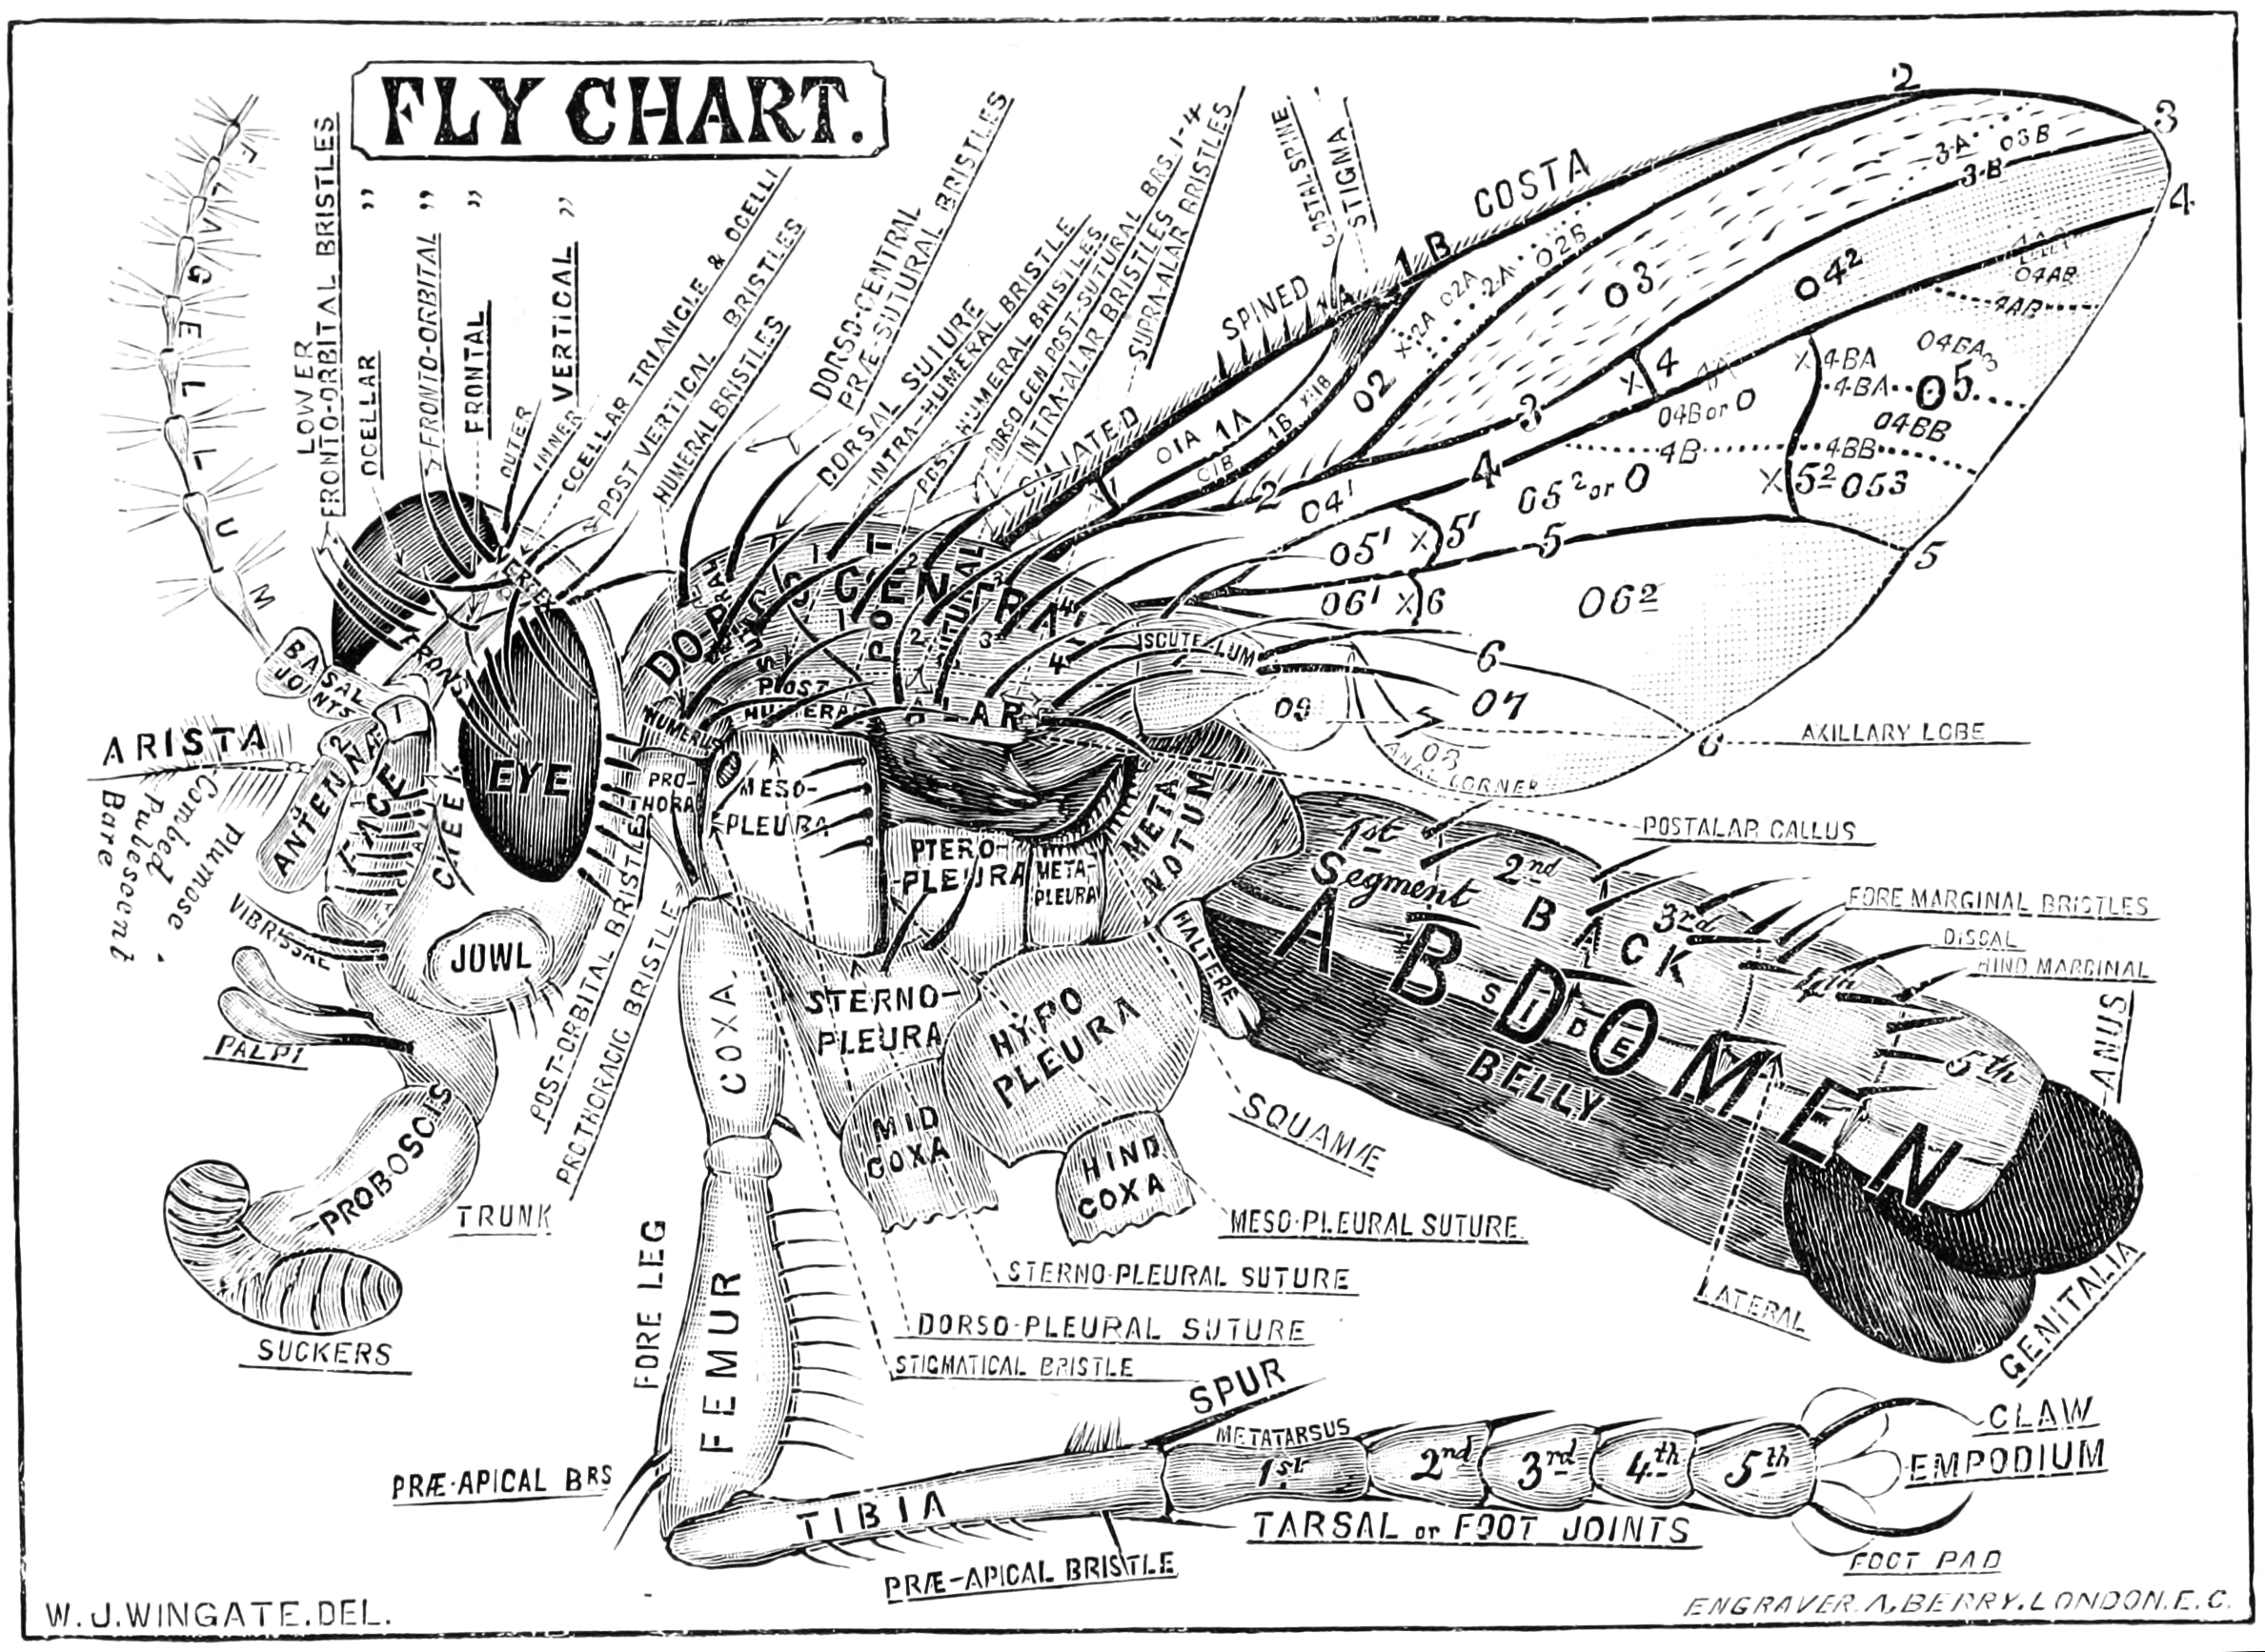
\includegraphics[width=0.84\textwidth]{morphology/flyAnatomy}
  \label{fig:flyAnatomy}
\end{figure}

In this lab we will observe specimens from across the phylogeny of Arthropoda, with an emphasis on Insecta. The goal is to familiarize yourself with the anatomical concepts relevant to most diagnostic keys and phylogenetic studies and to learn the various terms applied to these structures. Terms you should be comfortable with are differentiated by this \latinword{font}.

There is no single, perfect reference for insect anatomy and function. The treatise by \cite{snodgrass1935principles}, however, is a tested classic, which, despite being quite out of date regarding evolutionary hypotheses, covers most of the anatomy relevant to taxonomy. \cite{beutel2013insect} is a more contemporary treatment of insect morphology, with an emphasis on the phenotypes most relevant to our understanding of hexapod relationships.

\section{Methods}
Working with a partner, organize your space, specimens, tools, and microscope. Probes and forceps are available to manipulate the specimens. Some specimens may be available for dissection and more destructive observation; these will be clearly labeled (\textit{i.e.}, don't assume you can dissect just any specimen). Annotate the figures below and draw as many parts as possible in your notebook, from many different kinds of arthropods. Learn the \latinword{highlighted} words and be prepared to define them on an exam.

\section{Orientation}
Before we start looking at specific body parts take a few minutes to observe the specimens before you. Manipulate them with your forceps and probe under the microscope. Take some time to understand the biospatial concepts: \latinword{anterior}, \latinword{posterior}, \latinword{dorsal}, \latinword{ventral}, \latinword{lateral}, \latinword{proximal}, and \latinword{distal}. Label figure \ref{fig:biospatial} with these terms.\vspace{3mm}

\begin{figure}[ht!]
  \centering
    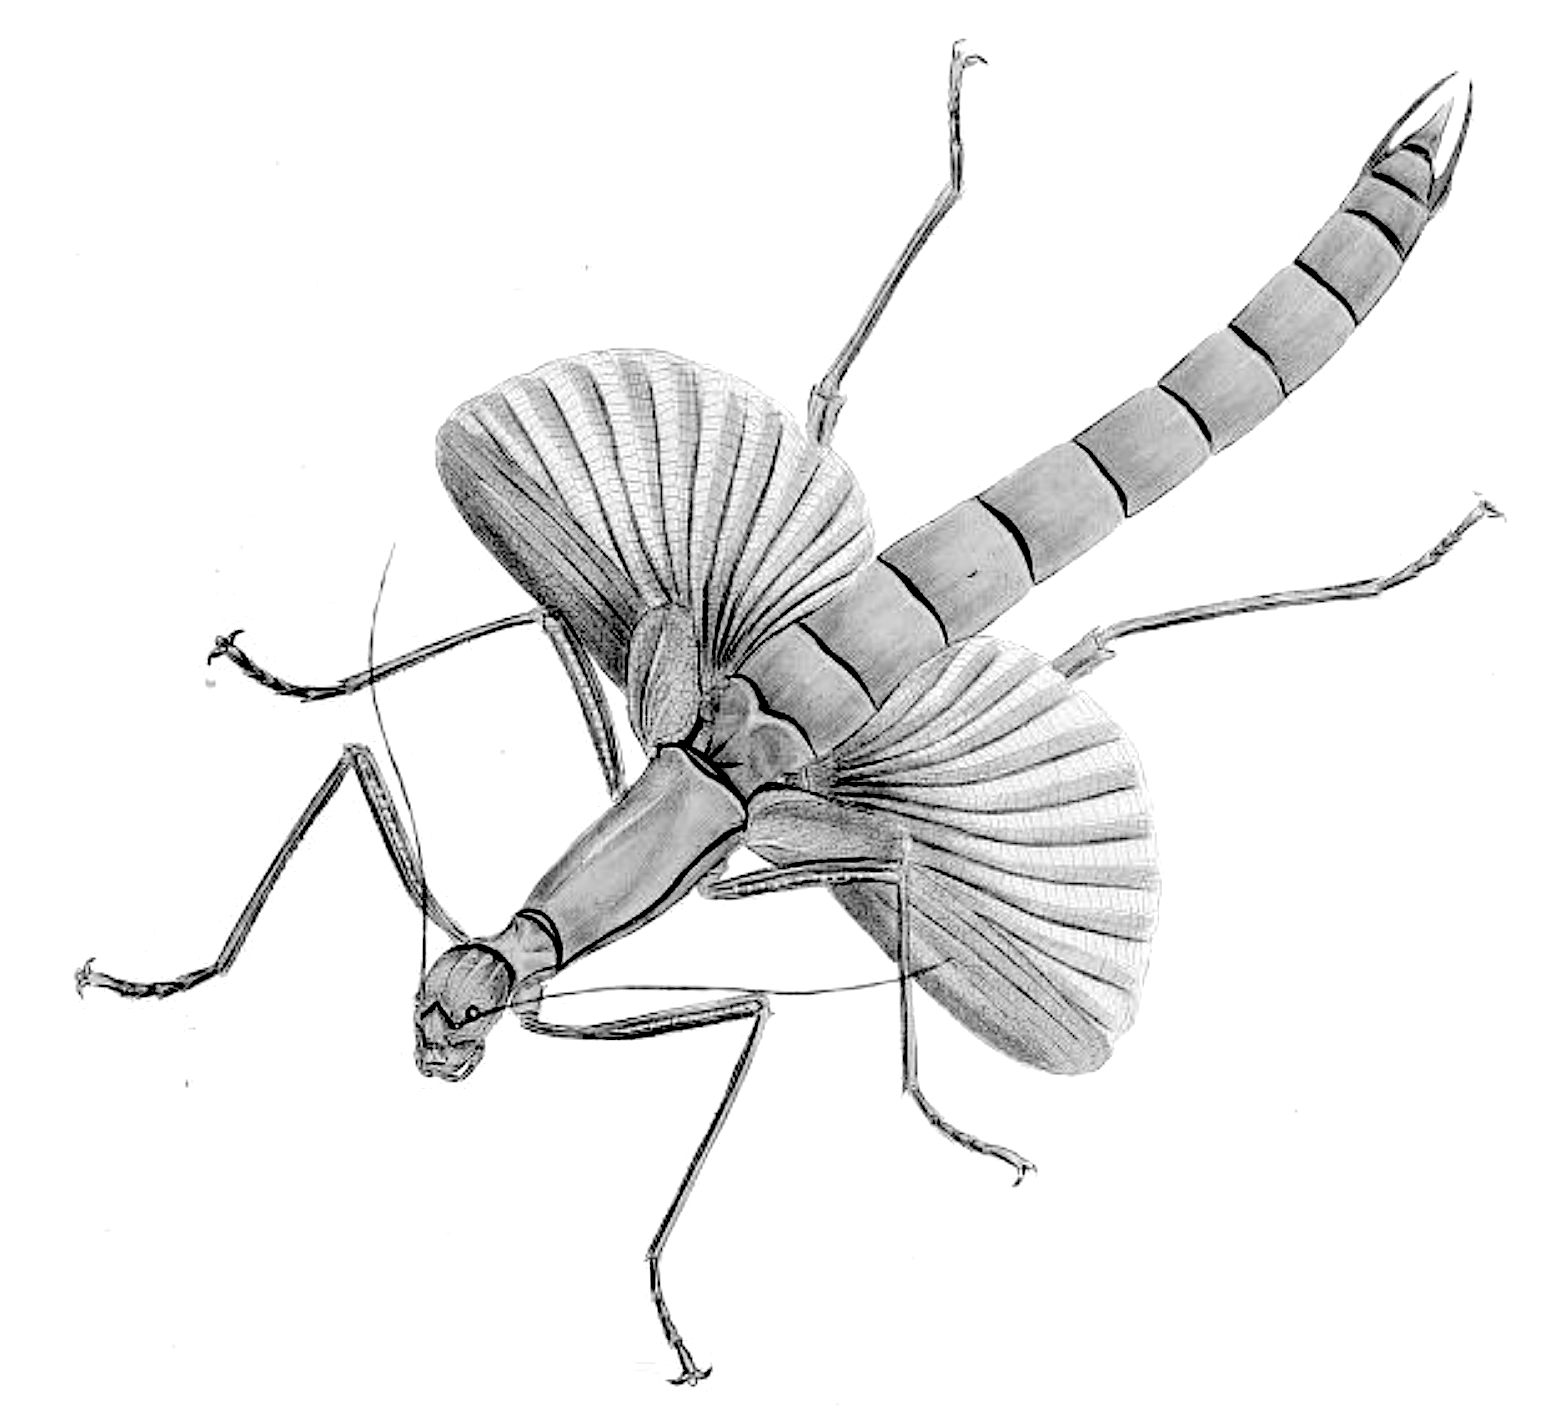
\includegraphics[width=0.55\textwidth]{morphology/biospatial}
  \caption{Phasmatodea \citep[][Plate X]{bhlitem104661}}
  \label{fig:biospatial}
\end{figure}

\begin{theo}
{}Observe several specimens you think represent different branches of the arthropod tree---\textit{e.g.}, a spider, a millipede, a beetle, and a few others. Can you describe at least three traits these organisms have in common?
\end{theo}

\section{Segmentation}
\latinword{Segments} are \latinword{metameric} subdivisions of the body or of appendages. Some researchers use ``segment'' only for those metameric subdivisions that meet certain criteria, for example if they each have intrinsic musculature. Using your forceps and probe, try to expand and contract your arthropod specimens. Separate two \latinword{flagellomeres} (subdivisions of the apical segment of the \latinword{antenna}, the \latinword{flagellum}) and then the \latinword{pedicel} (the medial antennal segment) from the \latinword{scape} (proximal segment of the antenna) on one of the beetles.\vspace{3mm}

\noindent{}Try to separate two segments on the \latinword{abdomen} of a specimen. Observe the difference in stiffness between the \latinword{arthrodial membrane} and a \latinword{sclerite}. \vspace{3mm}

\noindent{}\latinword{Tagmata} (\latinword{tagma}, sing.) are body regions composed of several segments that function together for certain, specialized purposes.\vspace{3mm}

\begin{theo}[traits2]
{}How are appendage segments separated from each other? Keep in mind that the taxon name Arthropoda is derived from the Greek \textit{árthron}, ``joint'', and \textit{pous}, ``foot'', which together refer to their jointed legs.\vspace{3mm}

\noindent{}What components of the segment define the segment's boundaries? Arthrodial membrane is much more flexible than sclerites; why do insects and other arthropods need soft cuticle? Can you find and count the tagmata on different specimens? Compare an insect to a spider and a harvestman.
\end{theo}

\begin{figure}[ht!]
  \centering
    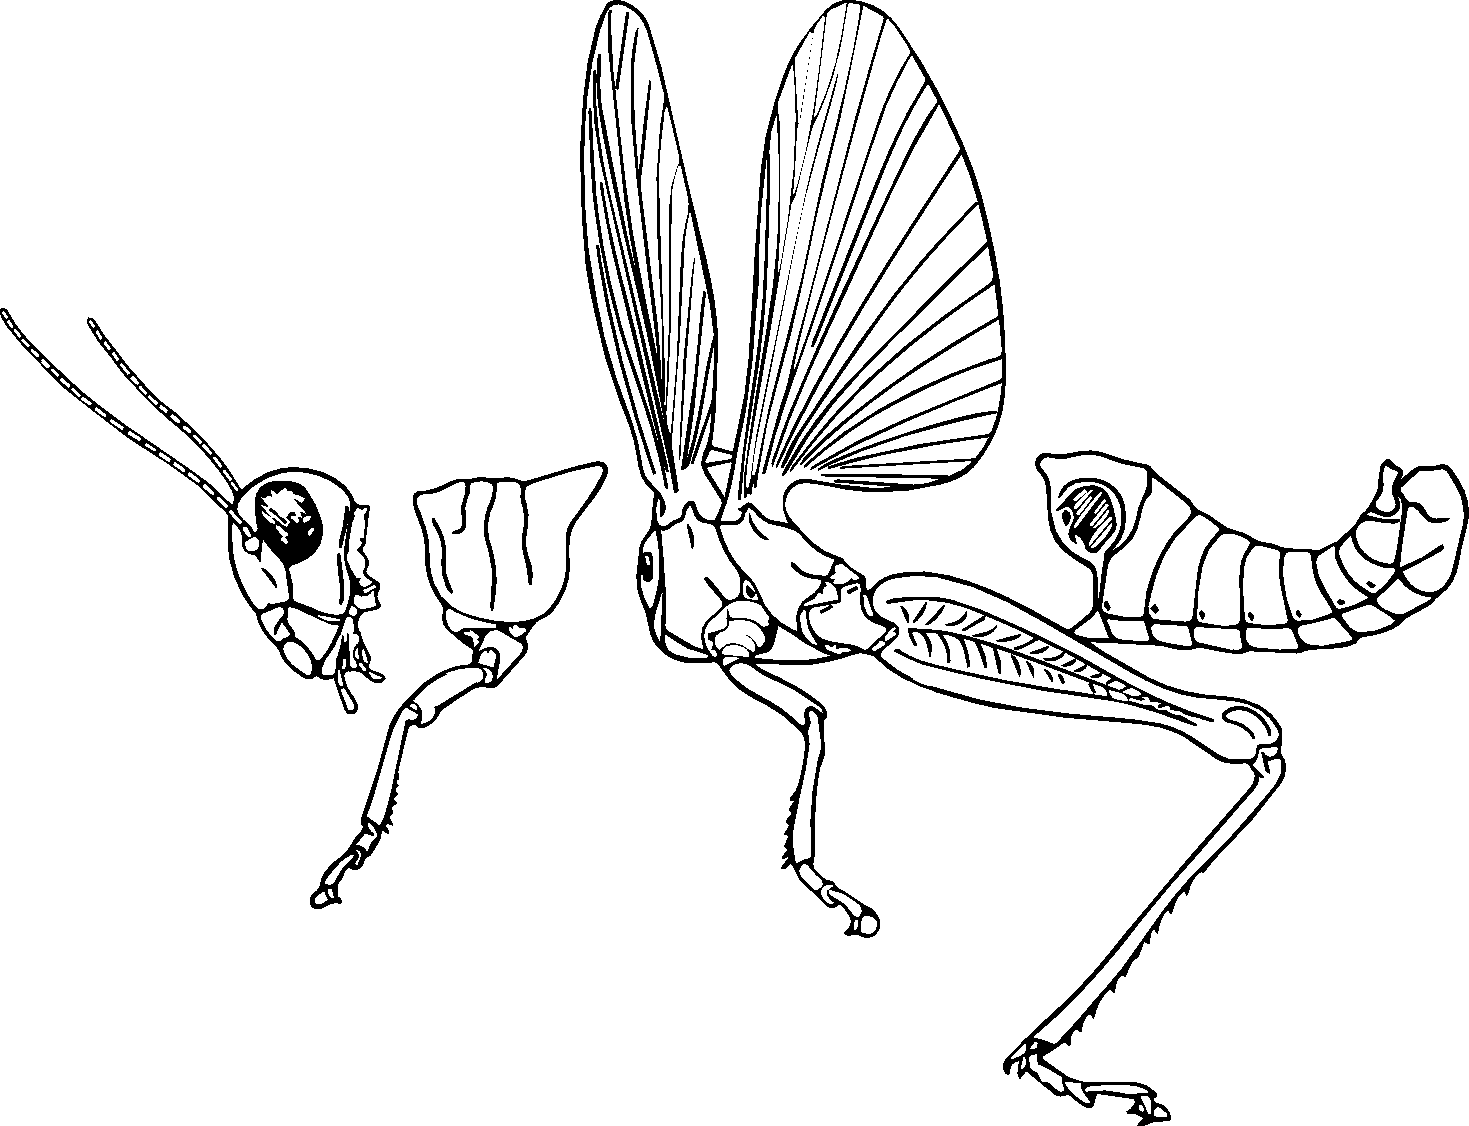
\includegraphics[width=0.7\textwidth]{morphology/Tagmata}
  \caption{Grasshopper. \citep[redrawn from ][Fig. 63]{bhl128276}}
  \label{fig:tagmata}
\end{figure}

\section{Appendages}
Each segment has \latinword{appendages} associated with it, at least ancestrally. Take a minute to familiarize yourself with the components of an appendage. \vspace{3mm}

\begin{theo}[appendage]
{}How would you define ``appendage''? Are wings appendages?
\end{theo}

\section{Head}
The first tagma we'll look at is the \latinword{head}. Spend some time examining the heads of your specimens, both of insects and of non-insects. Note the number and location of appendages and look for evidence of segmentation. \vspace{3mm}

\begin{theo}[traits3]
{}Compare multiple insect heads. How many segments comprise the head? Now look at the spider and harvestman. Do non-insect arthropods have the same head configuration as Insecta? What are the major functions of the head?
\end{theo}

\noindent{}The \latinword{antenna} is the most obvious metameric appendage of the head. As we have seen earlier, the flagellum of the insect antenna is not musculated (only the first two sclerites, the scape and the pedicel, which are true \latinword{appendage segments}, have muscle attachments). Some non-insect hexapods (like Collembola) and non-hexapod pancrustaceans have fully musculated antennae.\vspace{3mm}

\begin{theo}
{}How many antennae do insects have? What about spiders and crayfish? Some arthropods do not have antennae, while others have highly reduced antennae. How do these arthropods, like harvestmen (Opiliones), compensate for the lack of this useful structure? Why don't insects need a muscular flagellum? You observe different antenna phenotypes in your specimens. Why are antennae so diverse in shape?
\end{theo}

\noindent{}Let's focus on mouthparts, which are comprised of the other head appendages. When examining the insects in front of you, try to identify the following structures (figure \ref{fig:headCockroach} should help orient you): \latinword{labrum} (Lm), \latinword{mandibles} (Md), \latinword{maxilla} (Mx), \latinword{maxillary palps} (Plp), \latinword{lacinia} (Lc), \latinword{labium} (Lb), \latinword{labial palps} (Plp).\vspace{3mm}


\noindent{}Some of these appendages are \latinword{metameric}---\textit{i.e.}, they are subdivided into many ring-like sclerites. The number and shape of these sclerites can be diagnostic. \vspace{3mm}

\begin{figure}[ht!]
    \centering
    \begin{subfigure}[ht!]{0.3\textwidth}
        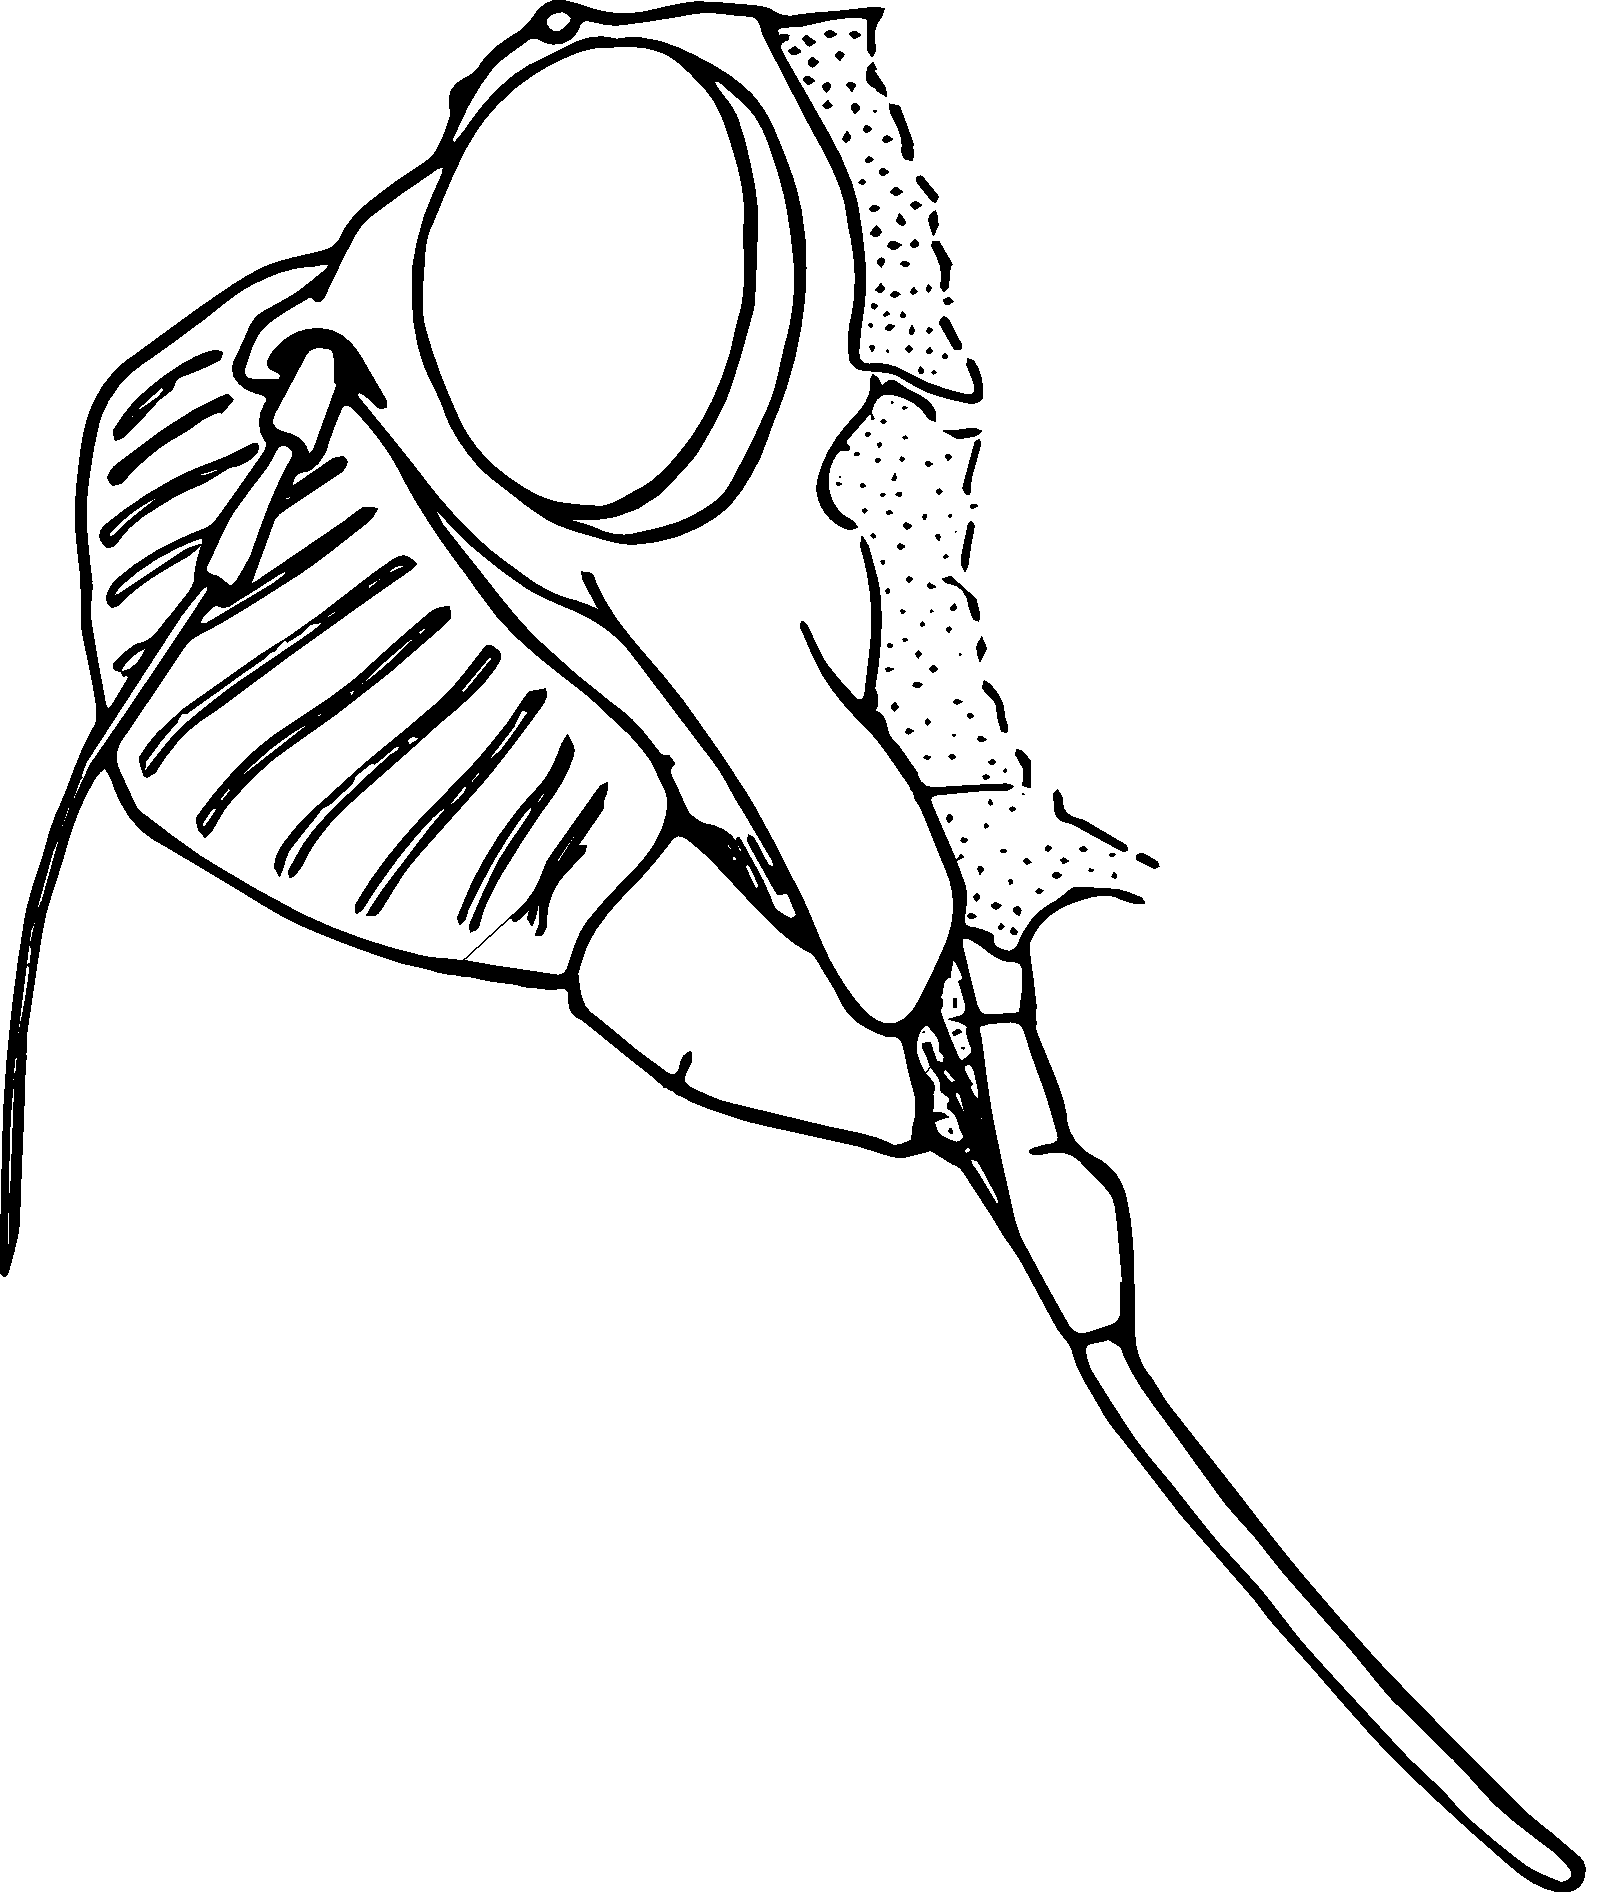
\includegraphics[width=\textwidth]{morphology/headCicada}
        \caption{}
        \label{fig:cicadaHead}
    \end{subfigure}
    \qquad
    \begin{subfigure}[ht!]{0.6\textwidth}
        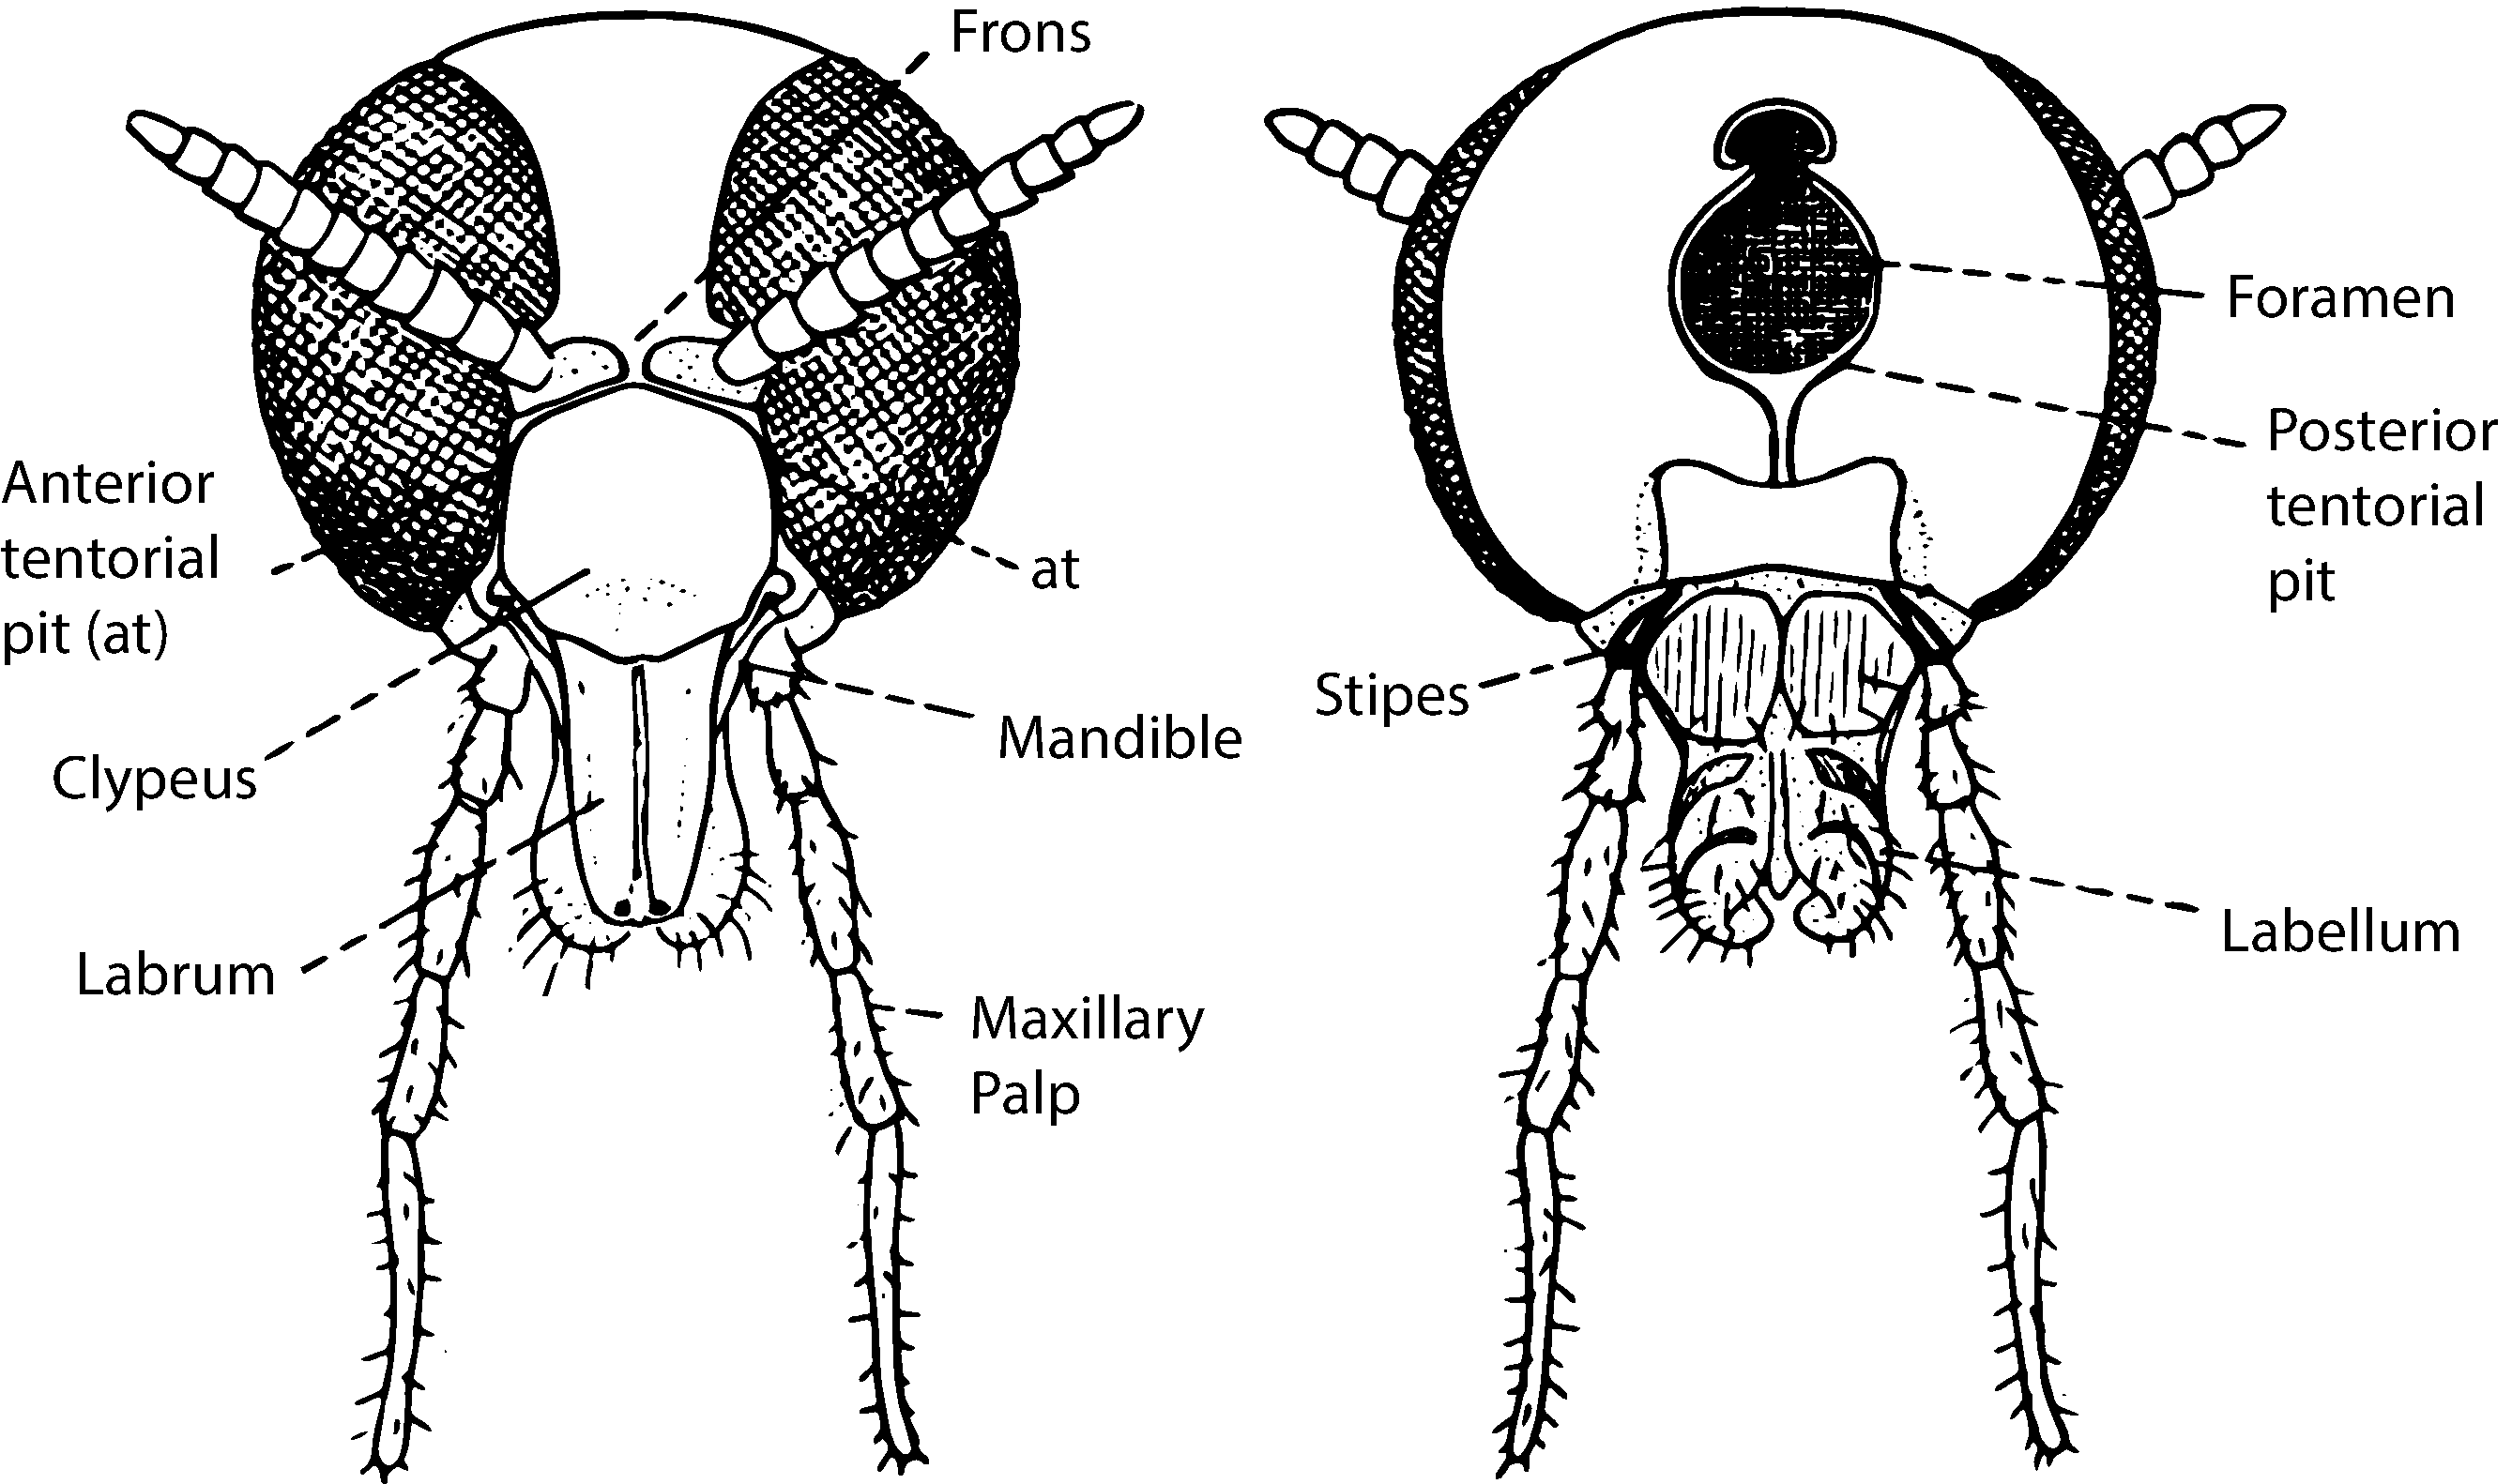
\includegraphics[width=\textwidth]{morphology/headFly}
        \caption{}
        \label{fig:headFly}
    \end{subfigure}
    \caption{Insect heads. \textbf{(a)} Cicada head \citep[redrawn from ][Fig. 121]{bhl128276}; \textbf{(b)} black fly head, anterior and posterior \citep[redrawn from][Fig. 24A,B]{snodgrass1944feeding}}
\end{figure}

\noindent{}Note the orientation of mouthparts in different specimens: projecting anteriorly\\ (\latinword{prognathous}), ventrally (\latinword{hypognathous}), or posteriorly (\latinword{opisthognathous}). These different orientations reflect modifications of the \latinword{cranium}. Find an example of each in your set of specimens.\vspace{3mm}

\noindent{}Once you're comfortable with insect mouthparts, see if you can understand the mouthparts of your arachnids.\vspace{3mm}

\begin{theo}[traits5]
{}What might be the function of the labrum, maxilla, and labium? Are these structures (plus the mandibles) present on all your specimens?\vspace{3mm}

\noindent{}Select the five arthropods you think have the greatest variation in mouthpart morphology: a fly, a bug, a spider, \textit{etc}. Describe and explain your hypotheses about the primary foods for each of these specimens? \vspace{3mm}

\noindent{}What might be the reason or function of these different mouthpart positions? How do these reflect their life history and habitats?
\end{theo}

\begin{figure}[ht!]
  \centering
    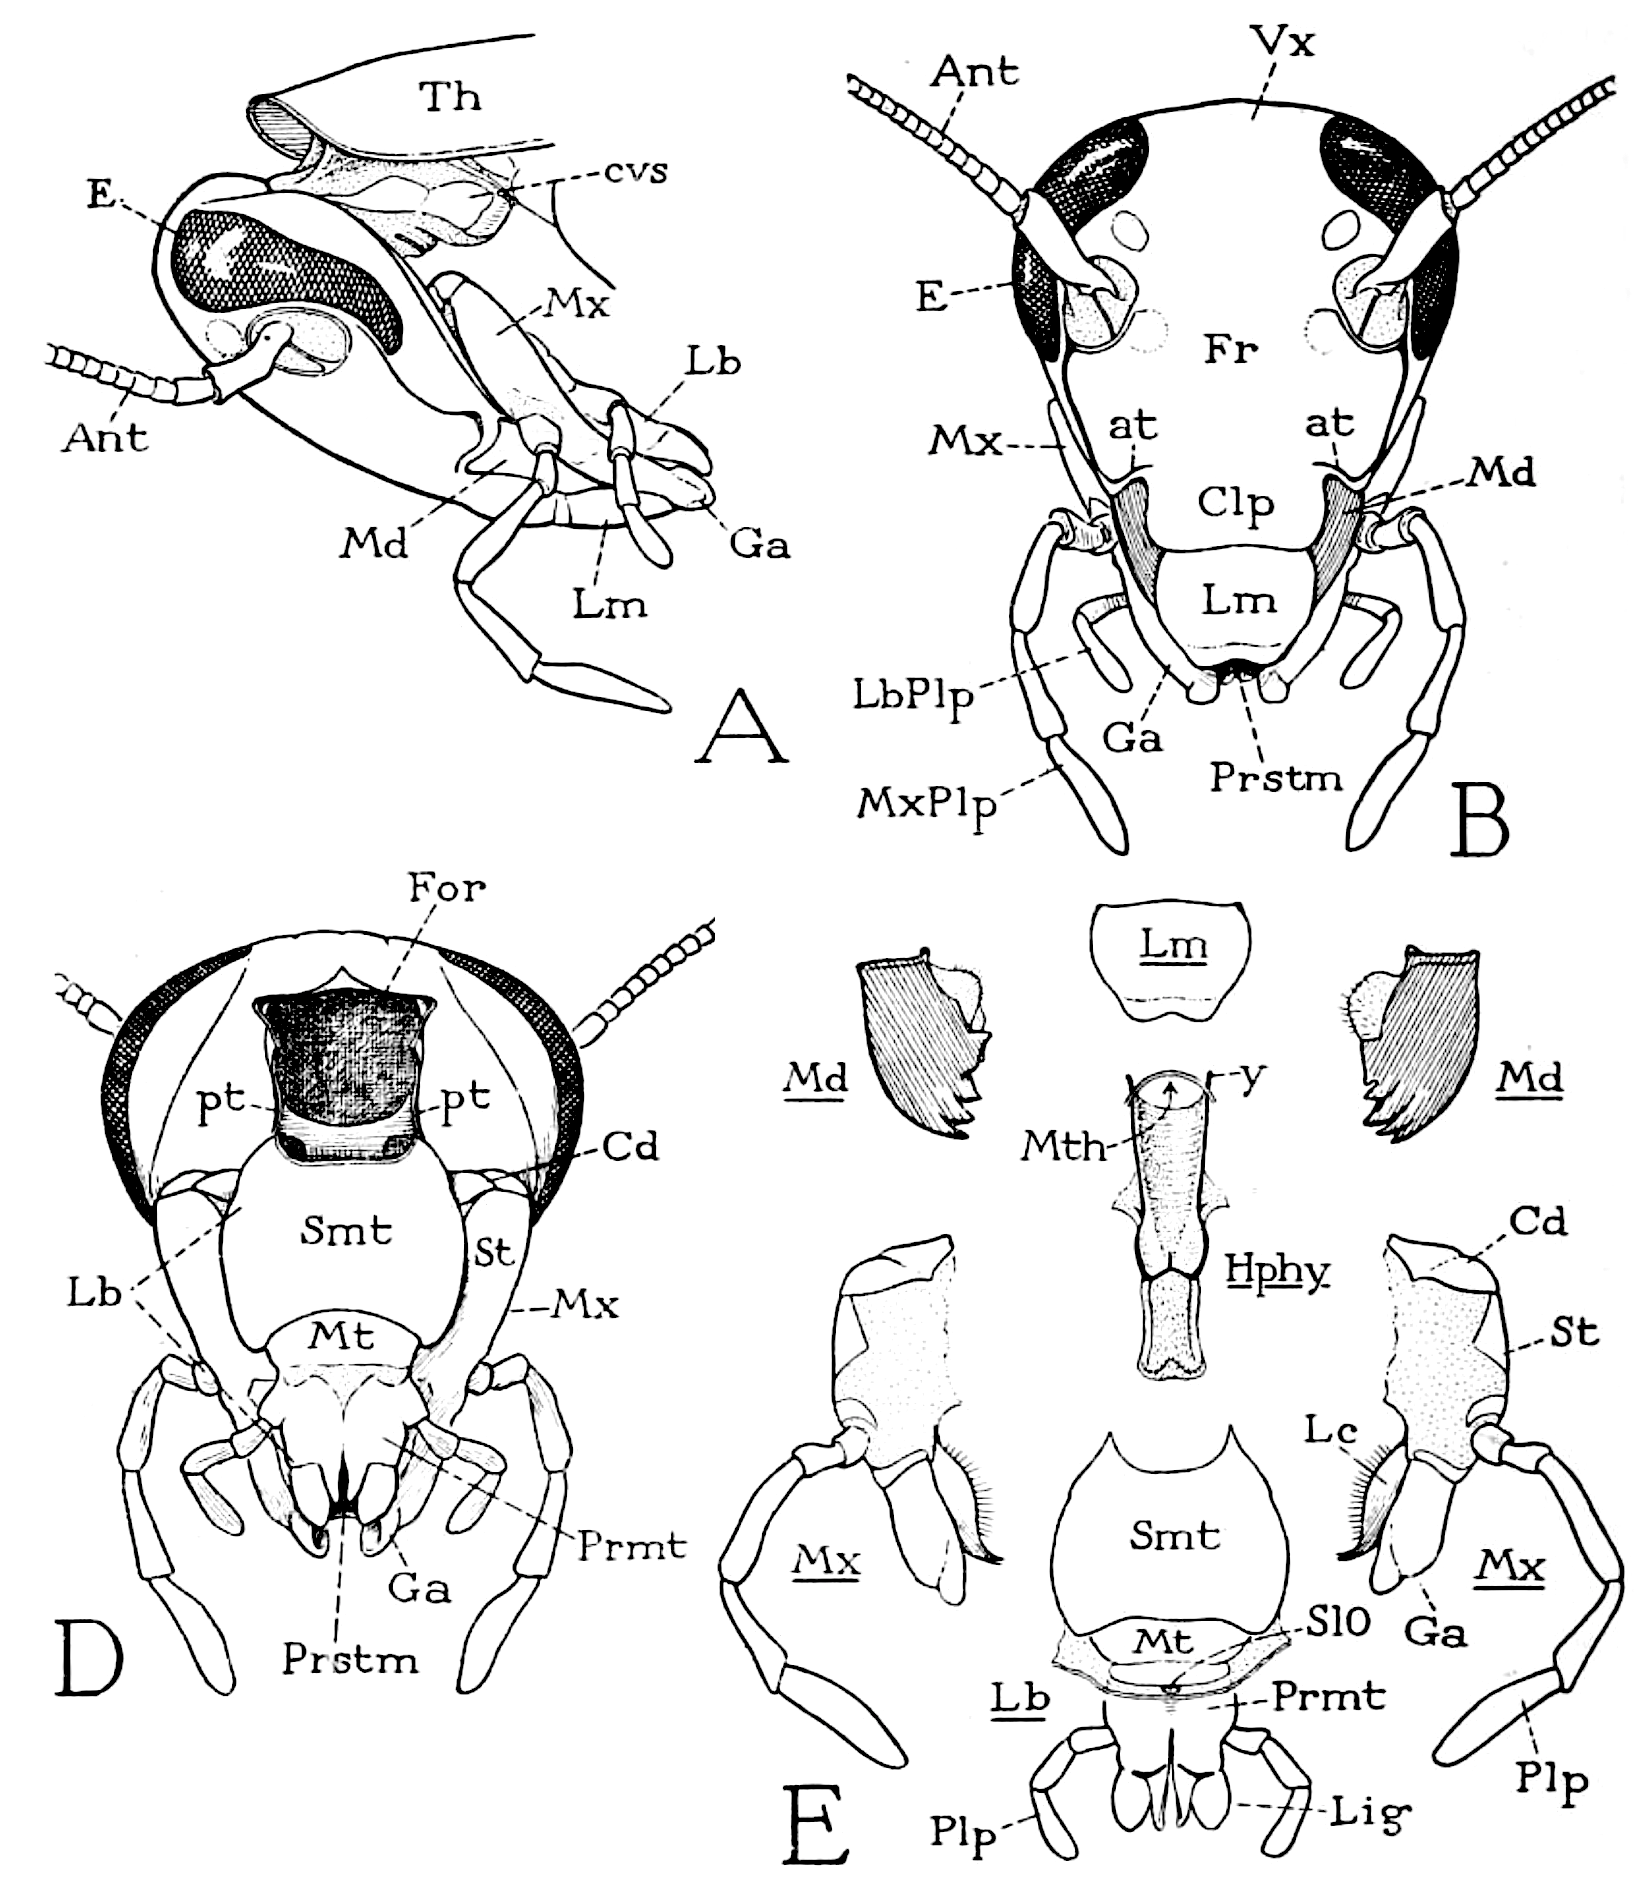
\includegraphics[width=0.7\textwidth]{morphology/headCockroach}
  \caption{Cockroach head. \citep[][Fig. 2A--E]{snodgrass1944feeding}}
  \label{fig:headCockroach}
\end{figure}

\noindent{}Eyes are used for vision and light detection. Locate them on your specimens and think about how they are differentiated from the rest of the body (cuticle). Compare the eyes of the insect specimens to those of non-insects.\vspace{3mm}

\begin{theo}[traits6]
{}What might be the function of a \latinword{compound eye} \textit{vs}. an \latinword{ocellus} (\latinword{-i})? How might spider vision differ from insect vision?
\end{theo}

\section{Thorax}
Posterior to the head is another tagma called the \latinword{thorax}. As with the head, examine each specimen for evidence of segmentation. See if each specimen even has a thorax. Compare a spider to an insect, for example. Try to determine how many segments comprise this tagma---you'll probably see three, the \latinword{prothorax}, \latinword{mesothorax}, and \latinword{metathorax}---and think about the tagma's primary function.\vspace{3mm}

\begin{theo}
{}In extant insects, the first thoracic segment does not bear a wing. Why? Does this body region serve other functions?
\end{theo}\vspace{3mm}

\noindent{}In your hexapod specimens, find sclerites you think represent the \latinword{notum}, \latinword{sternum}, and \latinword{pleuron}. Note that the surfaces of the nota of many insects have \latinword{furrows}, separating convex regions.\vspace{3mm}

\begin{figure}[ht!]
  \centering
    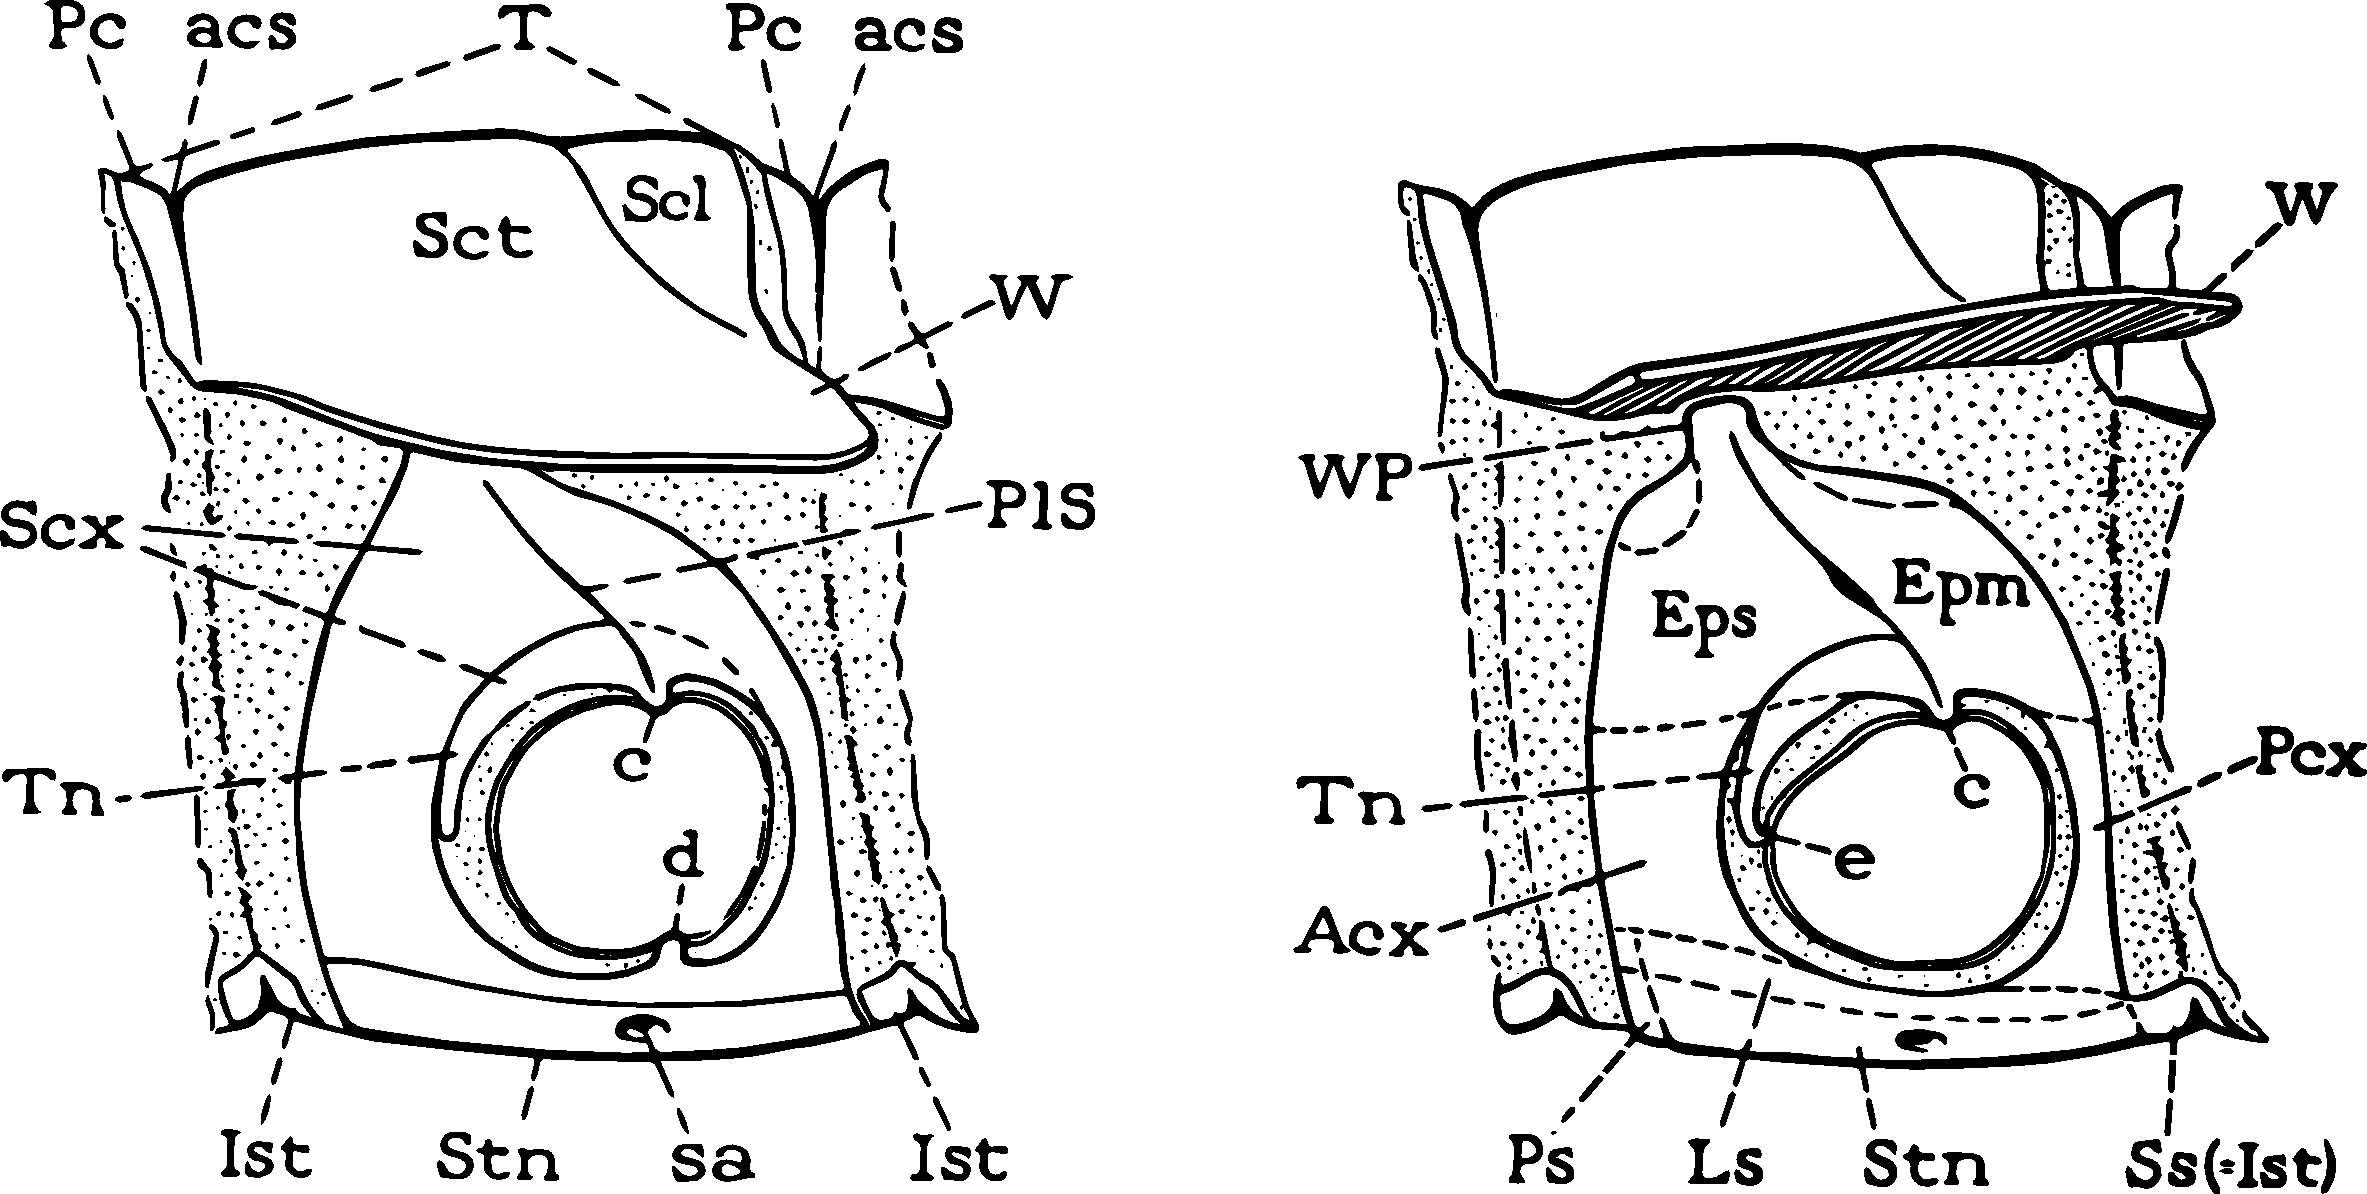
\includegraphics[width=0.8\textwidth]{morphology/scleritesThorax}
  \caption{Generalized thoracic segments, prothorax (left) and mesothorax (right). Antecostal suture (acs); dorsal (c) and ventral (d) subcoxo-coxal articulations; epimeron (Epm) episternum (Eps); eupleuron (Eupl); eutrochantin (Eutn); primary intersegmental line (Isg); intersegmental intersternites (Ist); precosta (Pc); scutum (Sct); scutellum (Scl); sternal plate (Stn); subcoxa (Scx); tergum (T); trochantin (Tn); wing process (WP). \citep[][Fig. 13]{snodgrass1929thoracic}}
  \label{fig:sclerites}
\end{figure}

\begin{theo}
{}Arthropods don't have ``bones''; where do muscles attach, to facilitate movement? Can you find evidence of your hypothesis by looking externally at the arthropod?
\end{theo}\vspace{3mm}

\subsection{Legs}

\noindent{}Locate the following leg segments in your insects: \latinword{coxa}, \latinword{trochanter}, \latinword{femur}, \latinword{tibia}, \latinword{tarsus}, \latinword{tarsomere}, \latinword{pretarsal claw}. Now try to locate these segments on the arachnid specimens. (Hint: try counting the leg segments, to see if they're the same between insects and arachnids). Spend some time observing different specializations of insect legs. We'll talk about adaptations related to locomotion and other behaviors. Some terms to define: \latinword{ambulatorial}, \latinword{cursorial}, \latinword{saltatorial}, \latinword{natatorial}, \latinword{fossorial}, \latinword{raptorial}, \latinword{chelate}. We'll also examine apices of various arthropod legs, to find structures (\latinword{attachment devices}) that help them cling to smooth surfaces, like a leaf or a window.\vspace{3mm}

\begin{figure}[ht!]
    \centering
    \begin{subfigure}[ht!]{0.5\textwidth}
        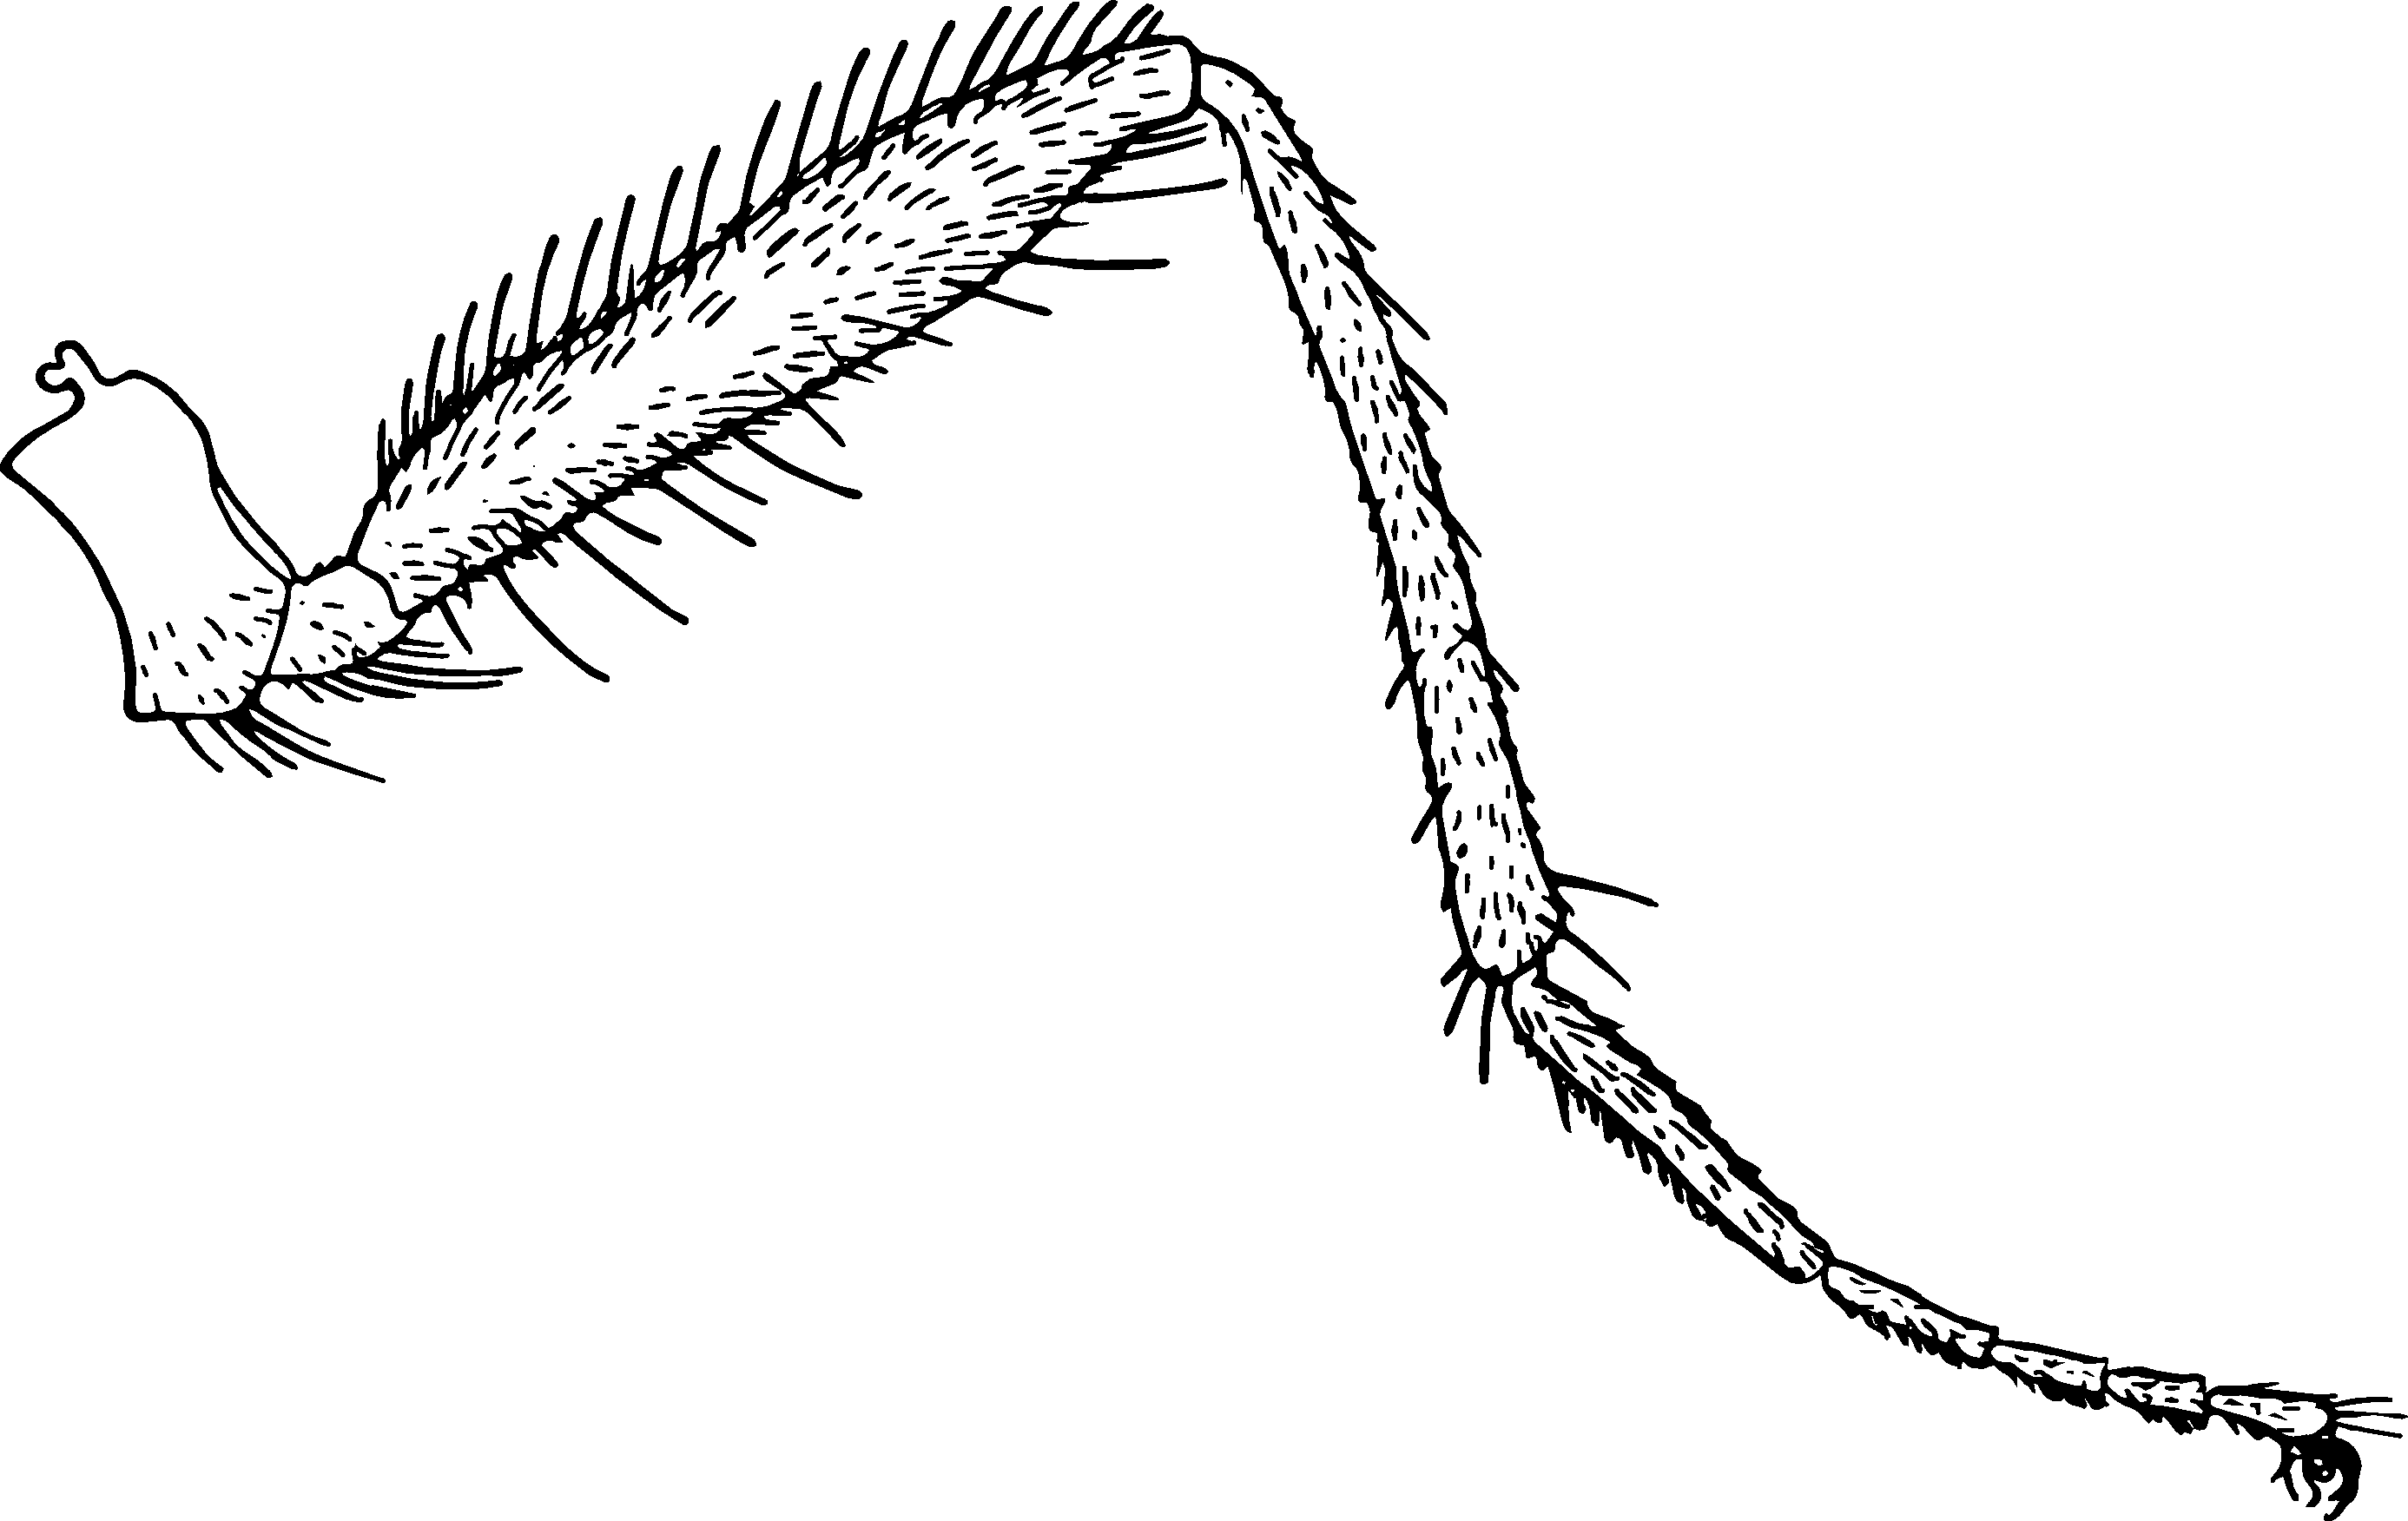
\includegraphics[width=\textwidth]{morphology/legSegments}
        \caption{}
        \label{fig:legSegments}
    \end{subfigure}
    \qquad
    \begin{subfigure}[ht!]{0.3\textwidth}
        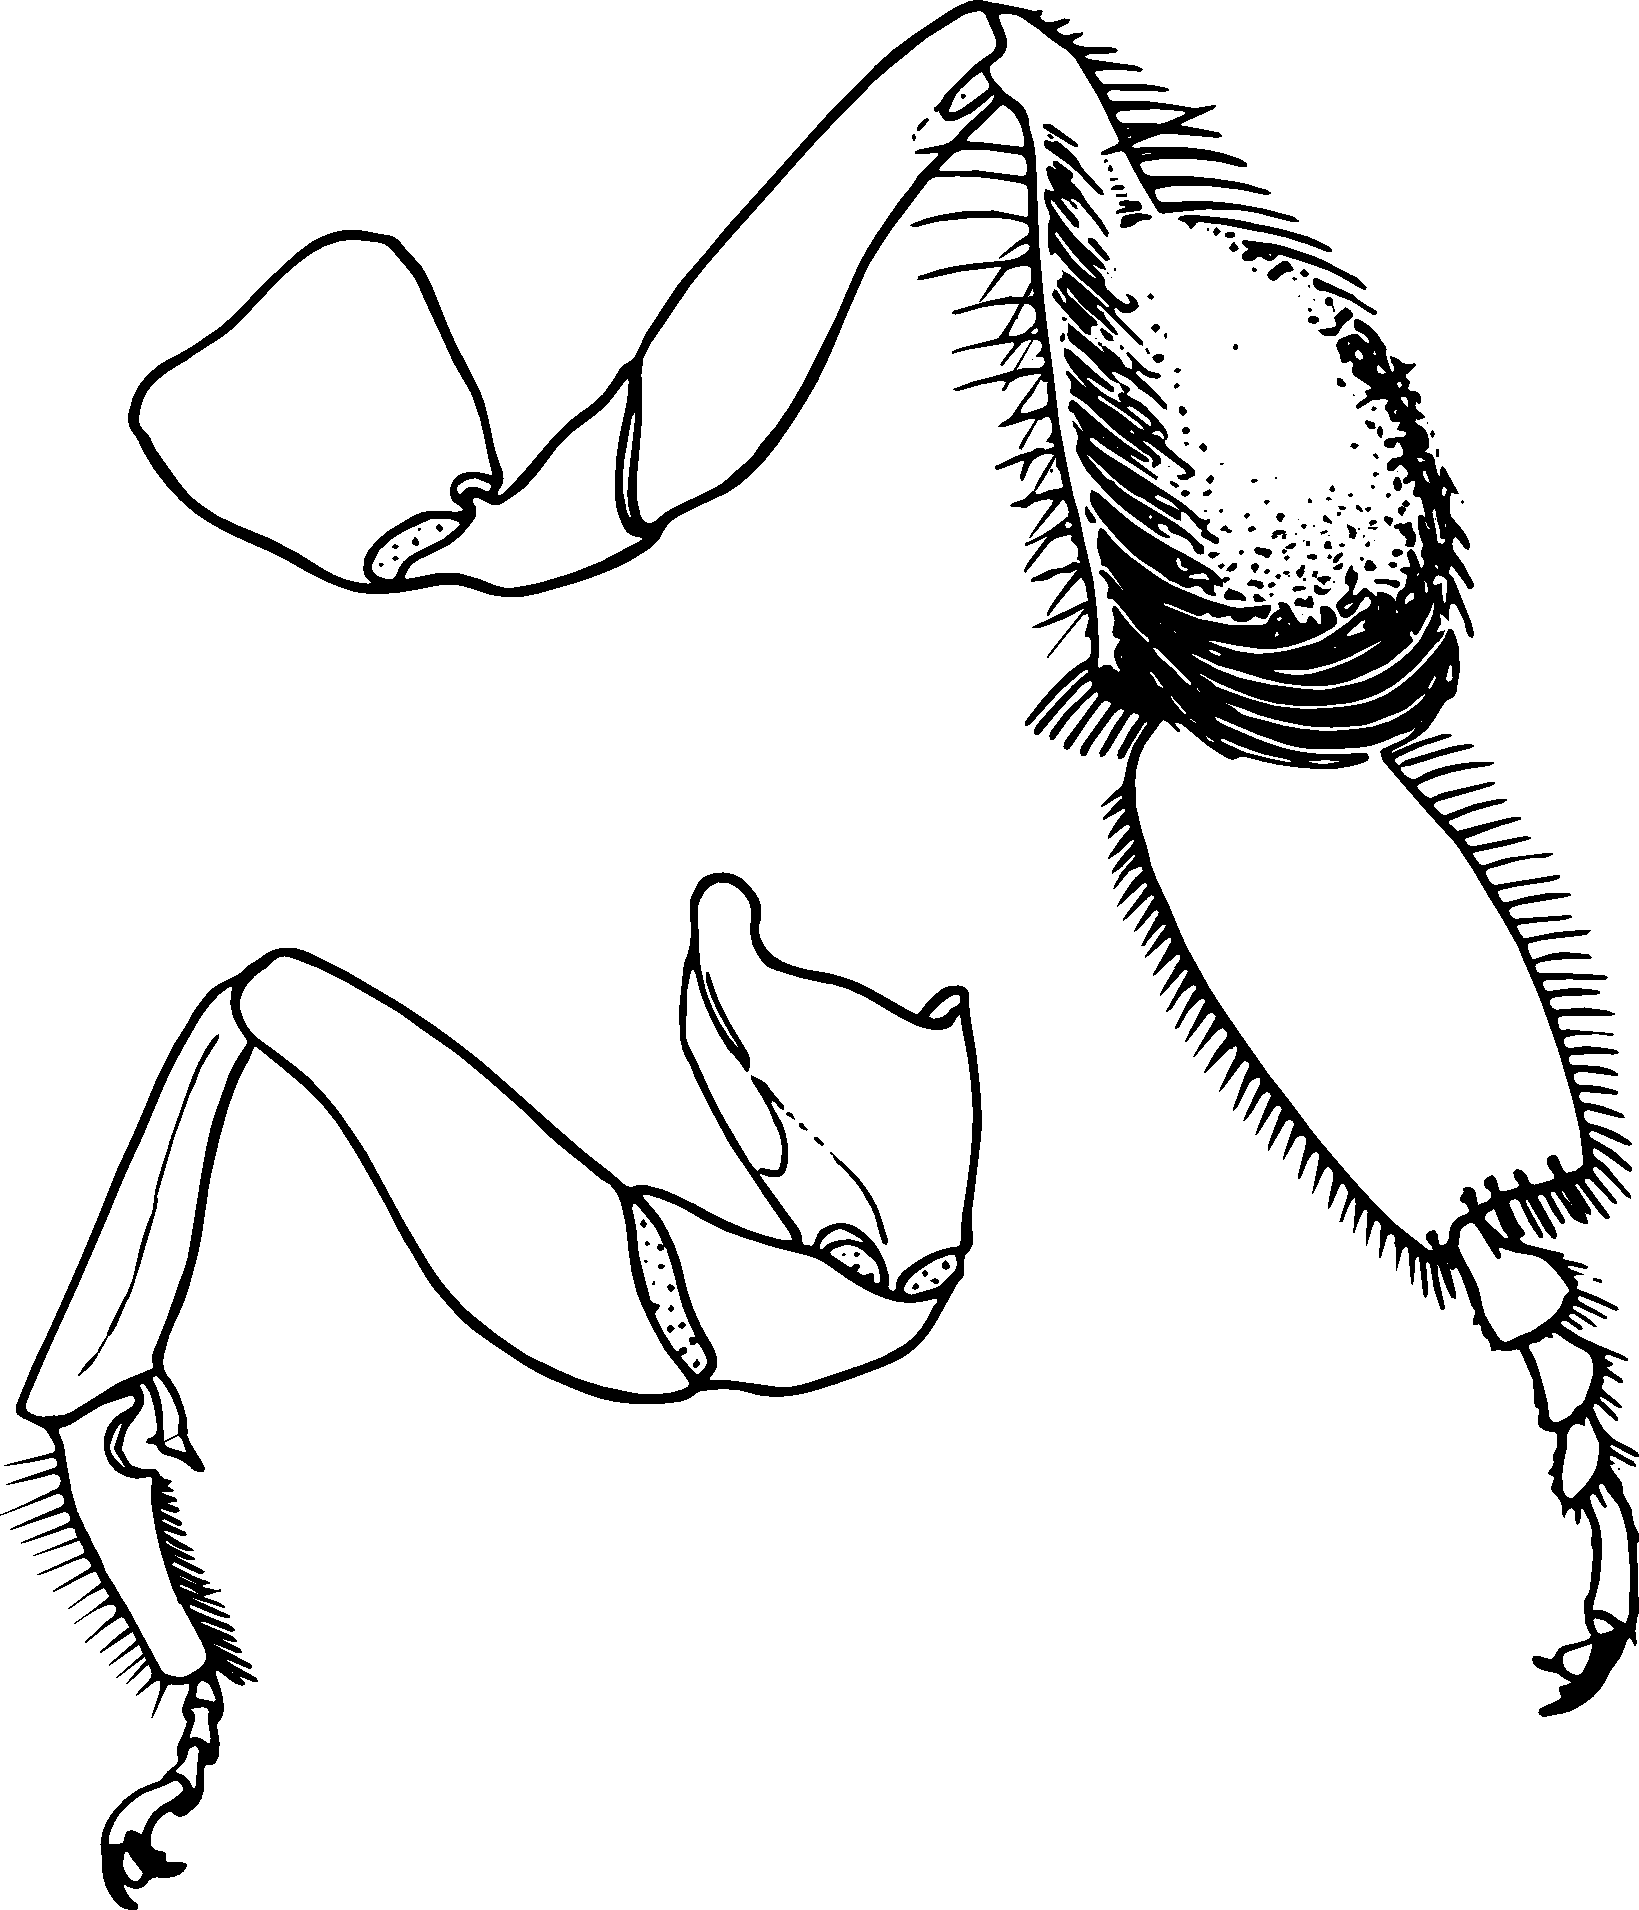
\includegraphics[width=\textwidth]{morphology/beeLegs}
        \caption{}
        \label{fig:beeLegs}
    \end{subfigure}
    \caption{Insect legs. \textbf{(a)} Aimple leg \citep[][Fig. 24, after Snodgrass]{bhlitem16791elementary}; \textbf{(b)} honey bee legs, hind (top) and fore leg (bottom) \citep[][Fig. 65]{bhl128276}}
\end{figure}%move the caption to here

\begin{theo}
{}Find at least 5 specimens with very different leg morphologies. Can you hypothesize something about the natural history of these specimens, based on their leg phenotypes?
\end{theo}\vspace{3mm}

\noindent{}Locate the \latinword{fore wing} and the \latinword{hind wing} on all your insect specimens. Then locate the following veins in different specimens: \latinword{costa} (C), \latinword{subcosta} (Sc), \latinword{radius} (R), \latinword{cubitus} (Cu), \latinword{medius} (M), \latinword{anal} (A). Look also for structures that aren't necessarily veins (fold lines, for example) but which otherwise aid in the function of the wing. Think about the characteristics and parts of the wings that allow them to function for flight.\vspace{3mm}

\begin{figure}[ht!]
  \centering
    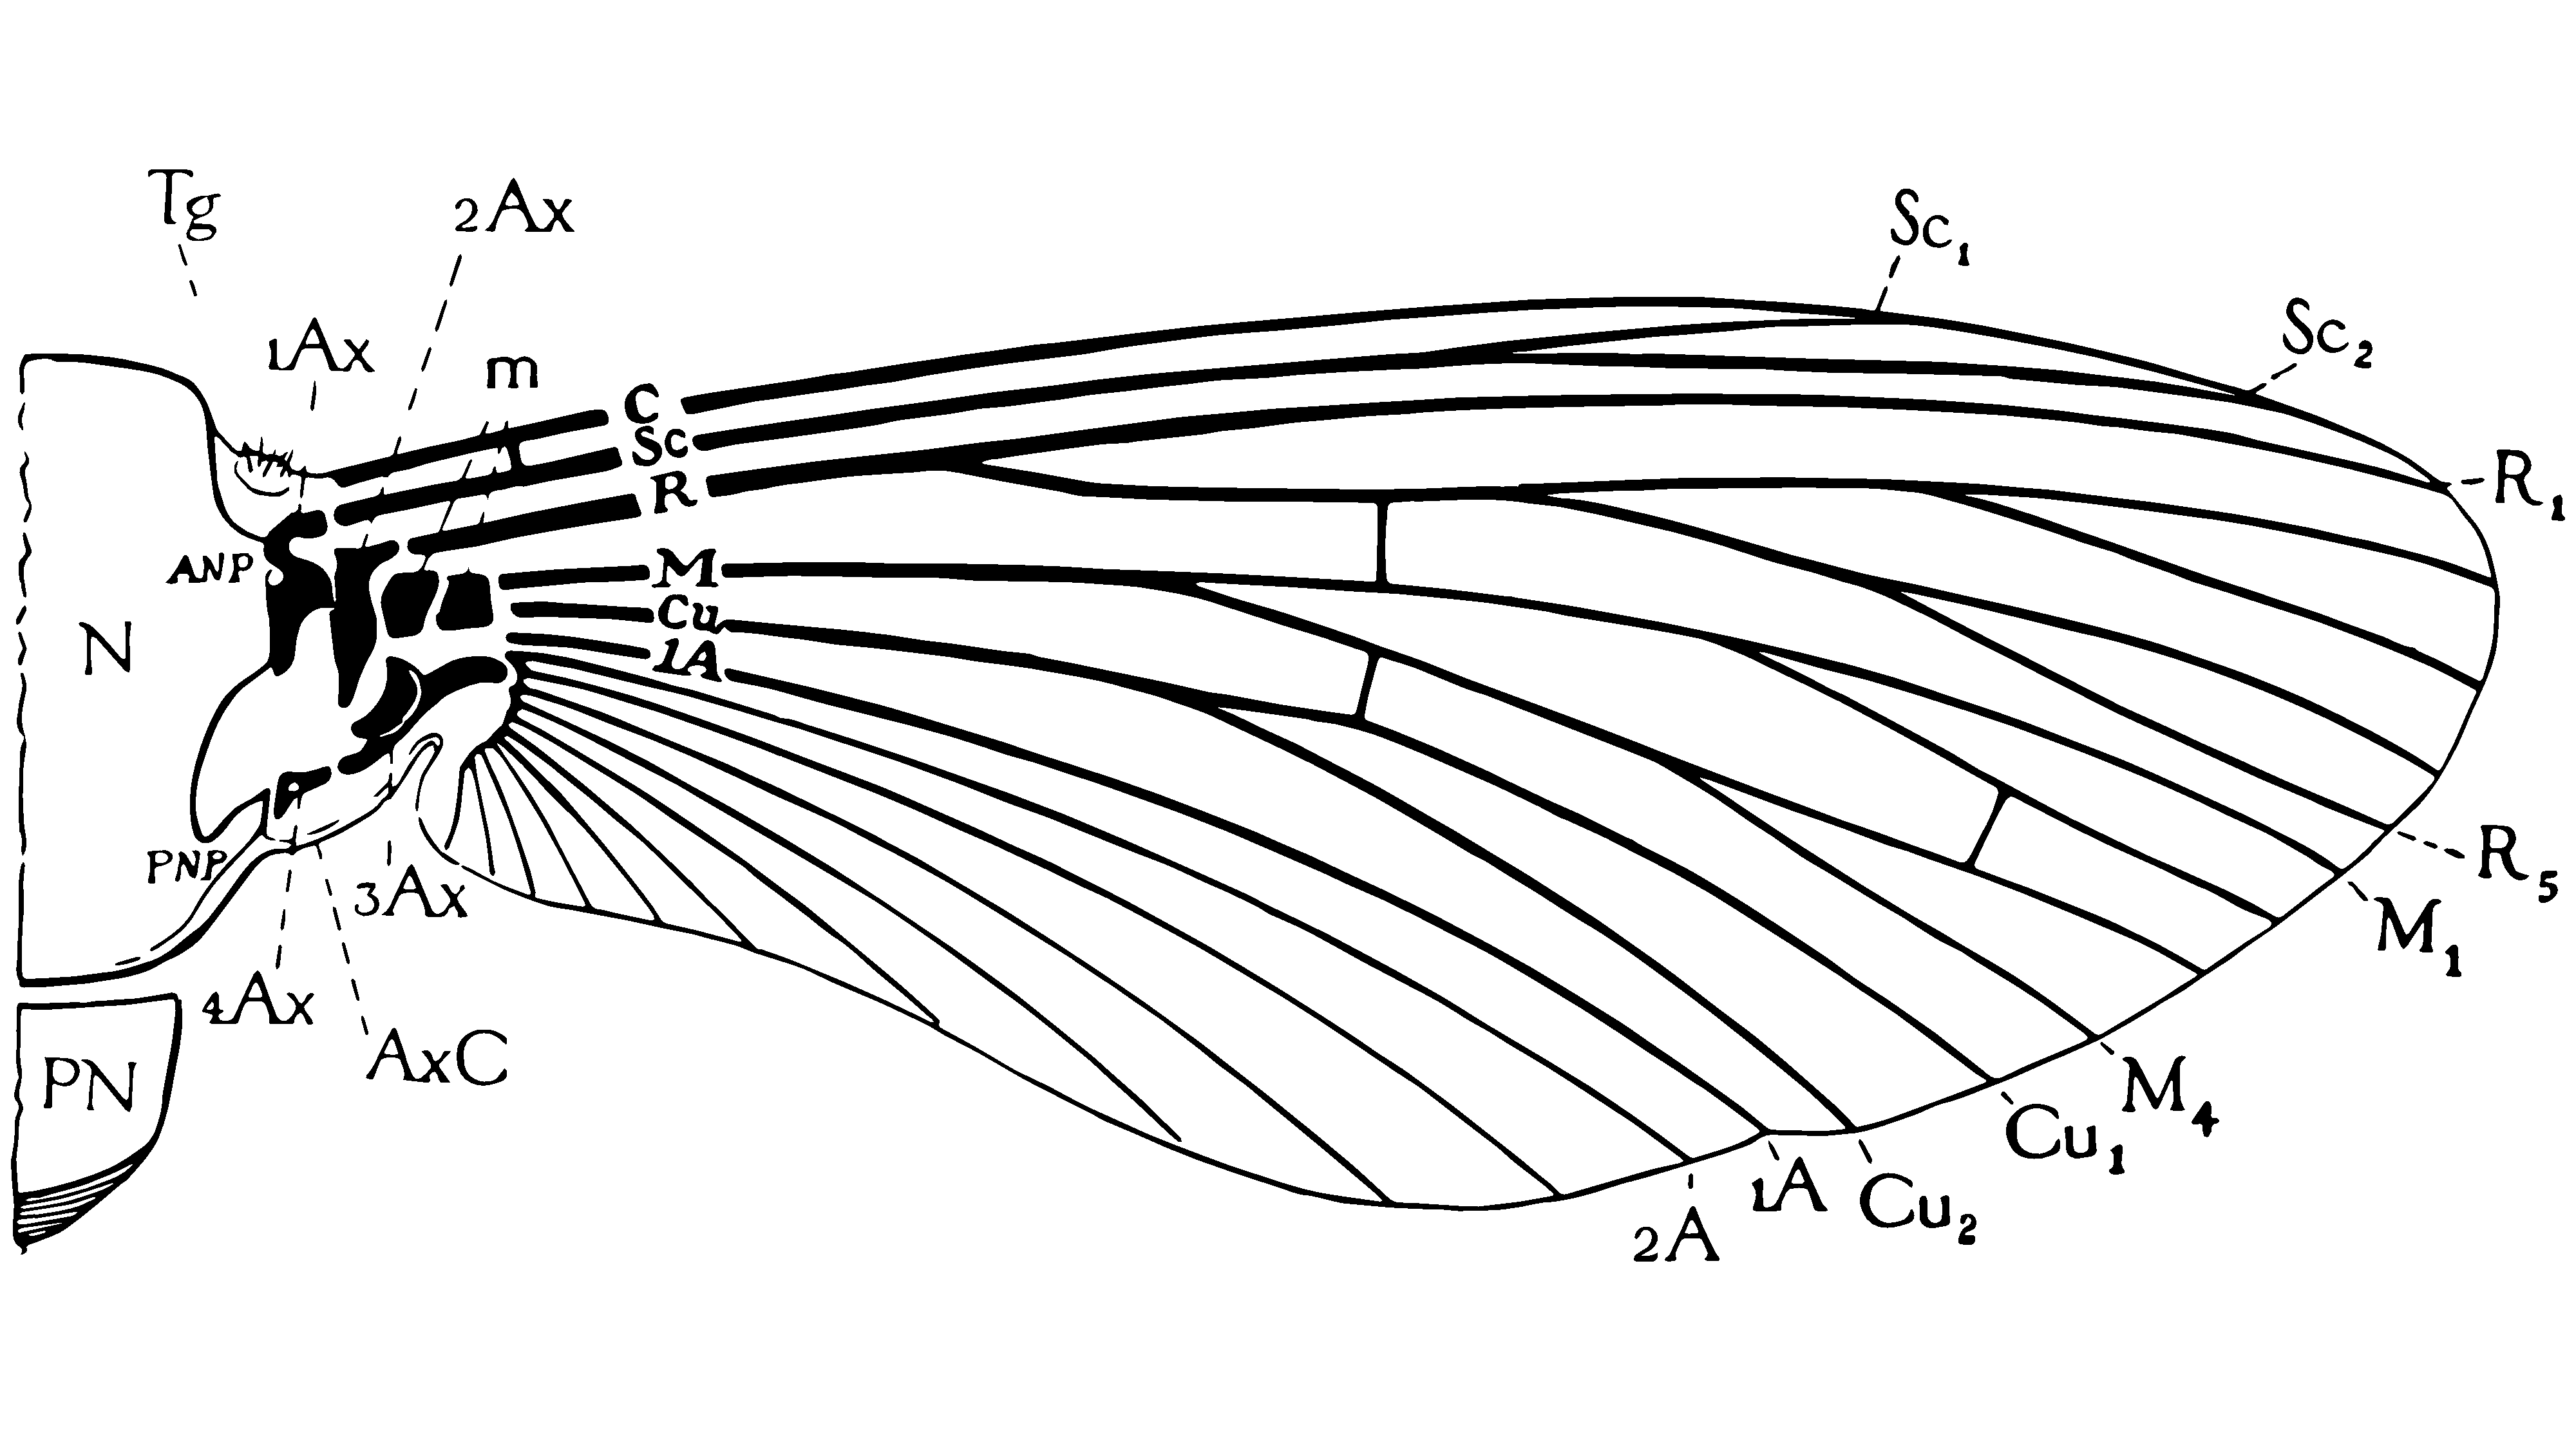
\includegraphics[width=0.8\textwidth]{morphology/wingveins}
  \caption{Generalized wing. \citep[][Fig. 6]{snodgrass1910honeybee}}
  \label{fig:wingveins}
\end{figure}

\begin{theo}
{}What might be the function of \latinword{wing veins}? Is it possible to homologize wing veins based on their orientation (relative to the anterior wing margin)? Do you see any patterns with respect to \latinword{crossveins} in your winged specimens?
\end{theo}\vspace{3mm}

\noindent{}Pay close attention to the wing morphology of beetles; we'll talk about the \latinword{elytron} (\latinword{-a}, plural). Given that the hind wing is so much larger than the elytron in your beetles, see if you can figure out how it fits under the fore wing.\vspace{3mm}

\noindent{}In some insects, Odonata for example, the fore and hind wings are used asynchronously during the flight. Hymenoptera, Lepidoptera, and some Heteroptera use the fore and hind wings simultaneously---\textit{i.e}., they function as a single wing. See if you can find anatomical structures that link or otherwise connect the two wings together.\vspace{3mm}

\section{Abdomen}
As with the tagmata above, see if you can find evidence for a third tagma posterior to the thorax---the \latinword{abdomen}---and for how many segments compose the structure.\vspace{3mm}

\noindent{}Look for appendages on the abdomen. Can you recognize male and female insects based on the tip of their abdomen? Think about the functions of the anatomical structures at the tip of the abdomen, for example the \latinword{cerci} (\latinword{cercus}, sing.) or the \latinword{ovipositor}.\vspace{3mm}

\begin{theo} 
{}The terminalia of the abdomen is key in species identification for numerous insect groups. Why?
\end{theo}

\begin{figure}[ht!]
  \centering
    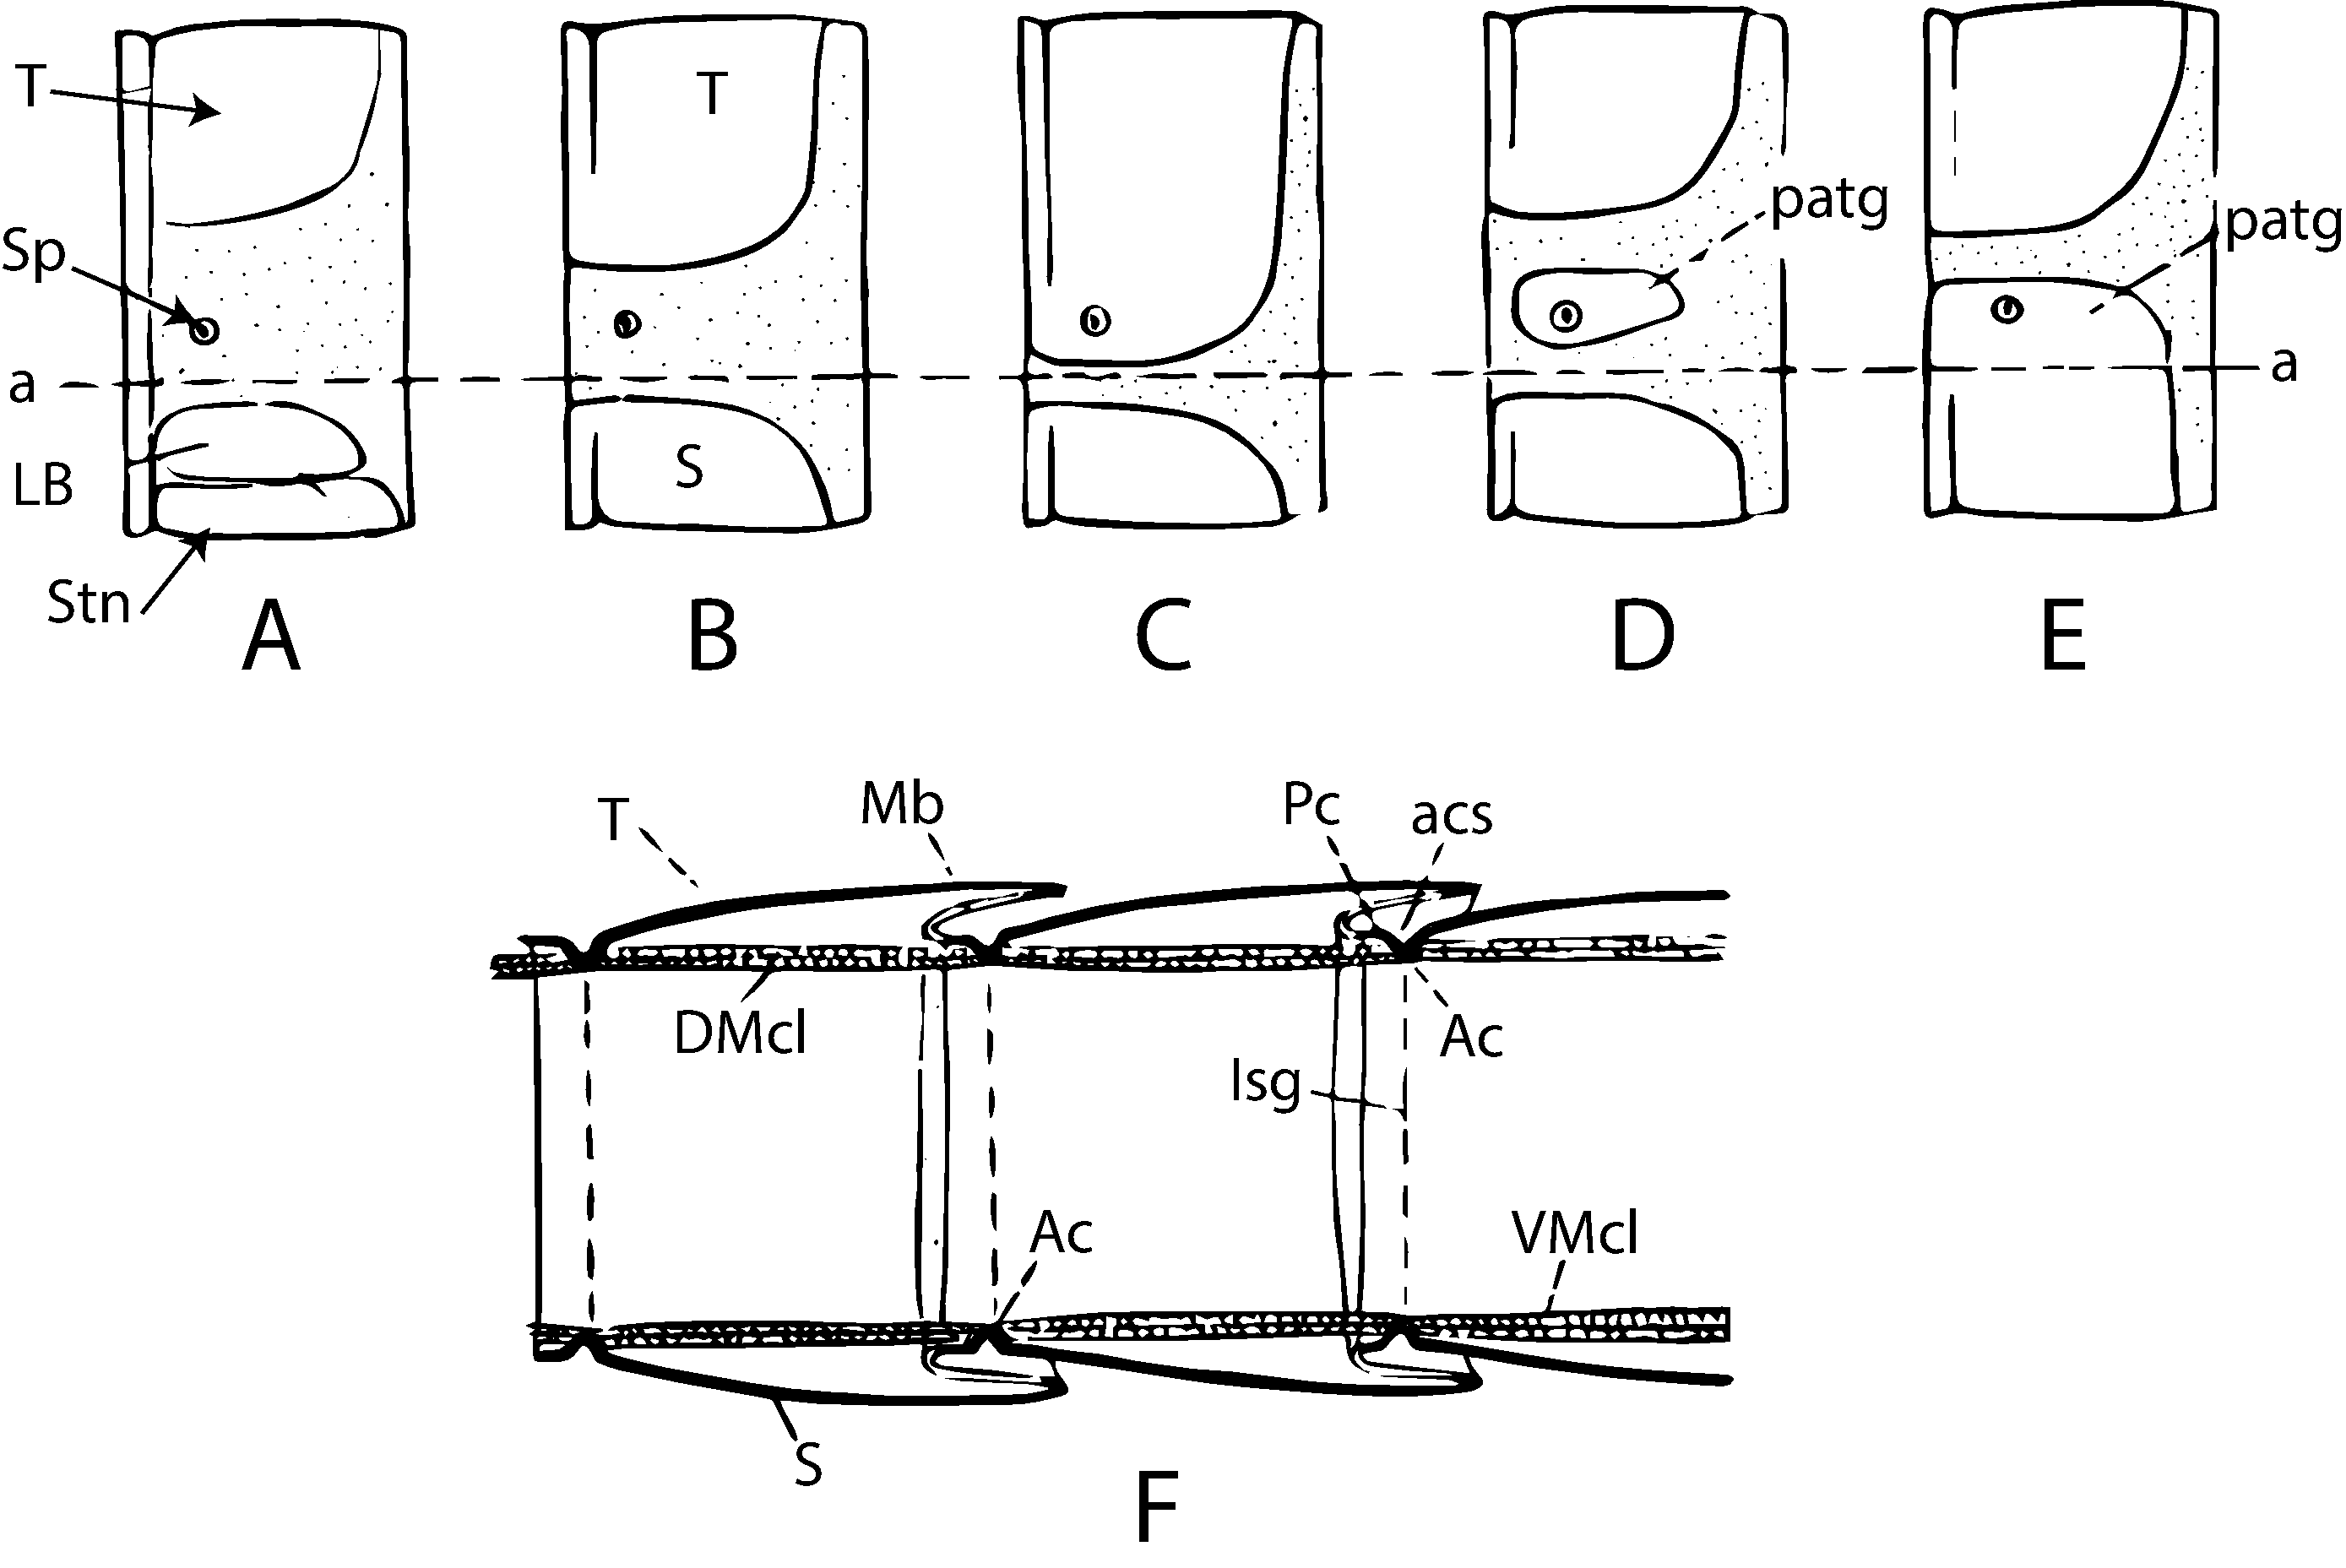
\includegraphics[width=0.7\textwidth]{morphology/abdomenSclerites}
  \caption{Abdominal sclerites. \citep[][Figs. 2A--F]{snodgrass1937morphology}}
  \label{fig:abdominalsclerites}
\end{figure}

\begin{figure}[ht!]
  \centering
    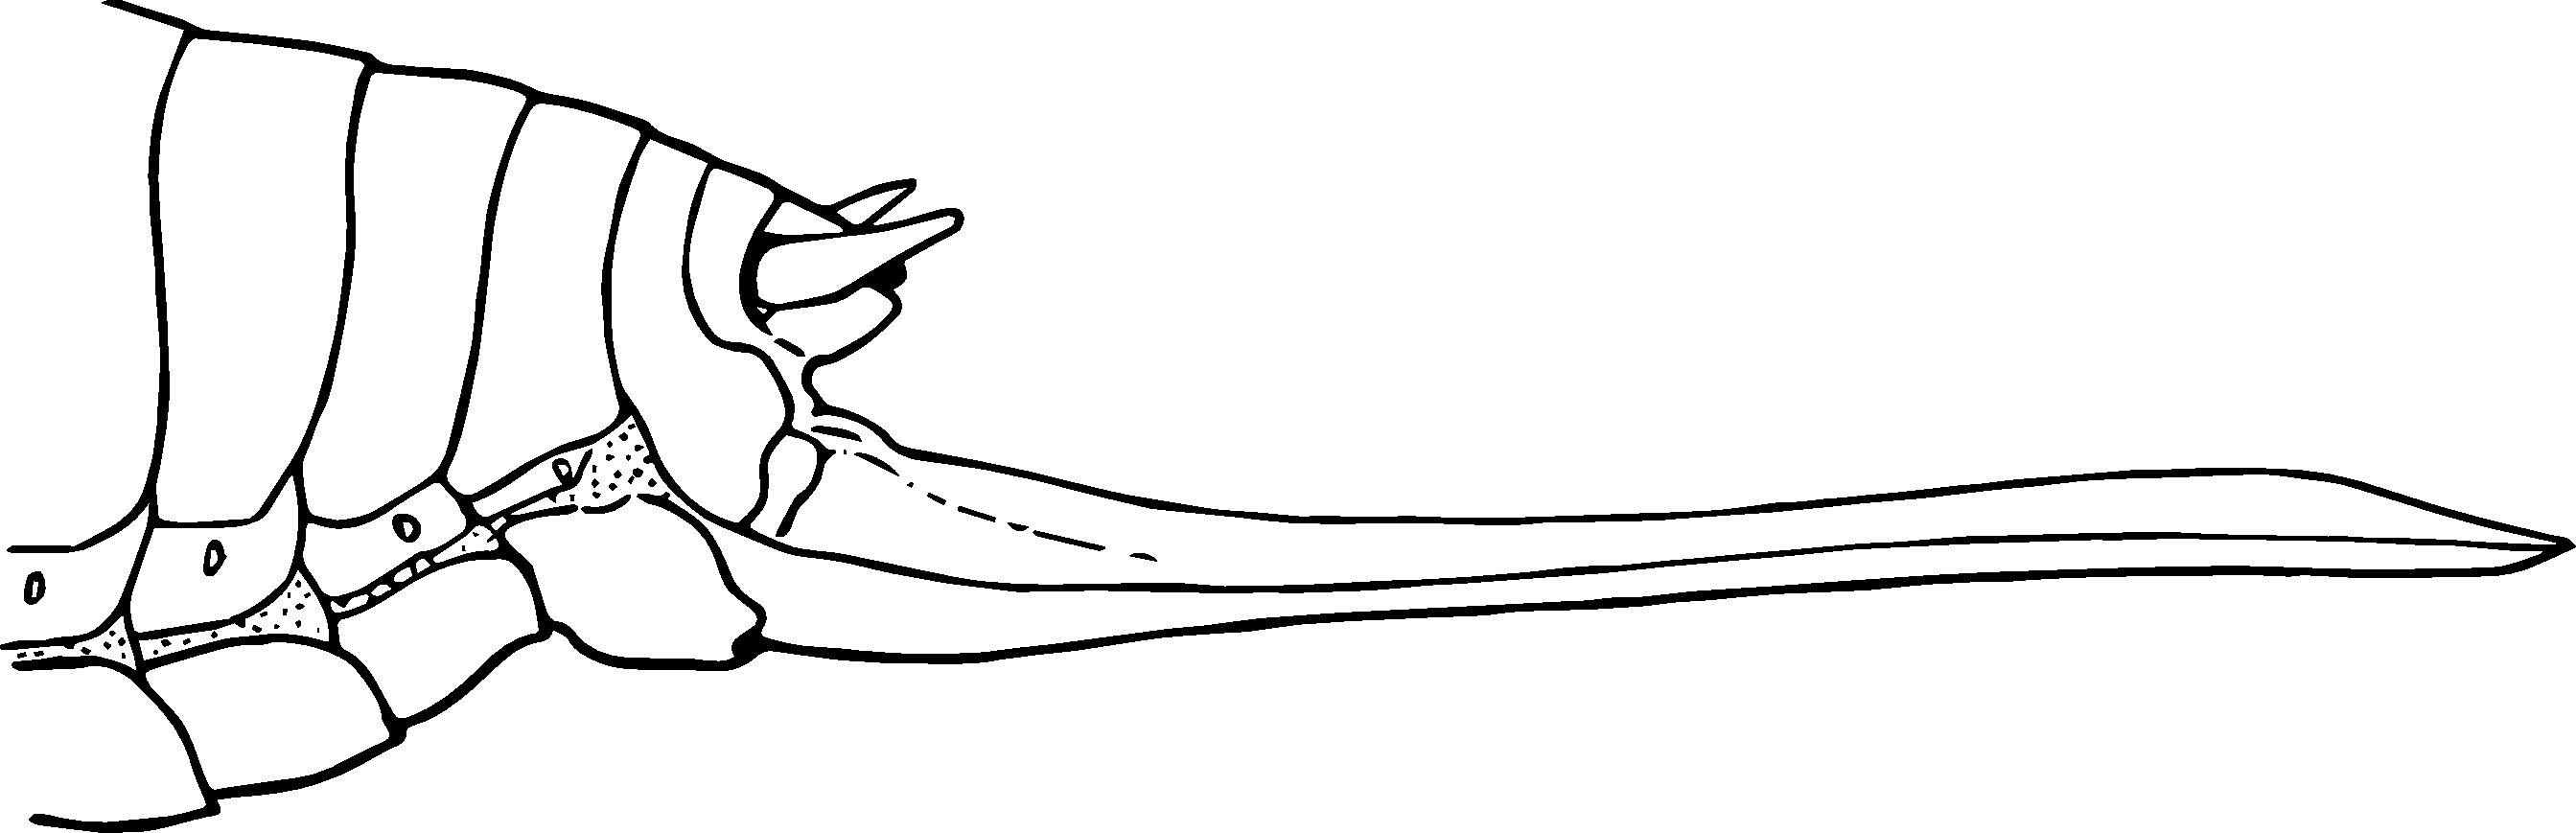
\includegraphics[width=0.7\textwidth]{morphology/ovipositor}
  \caption{Apex of female abdomen. \citep[][Fig. 74A]{bhl128276}}
  \label{fig:ovipositor}
\end{figure}

\noindent{}You should be able to see \latinword{spiracles} clearly on the abdomens of most insects. In most insects there are two sets of spiracles also on the thorax. Try to locate them in your winged arthropods, and then count the number of spiracles on the abdomen. Note that the second spiracle on the thorax is often difficult to find because it is located at the wing base.\vspace{3mm}

\begin{theo} 
{}Why is the abdomen generally softer and more flexible than the other tagmata? Why do we pin insects through the thorax?\end{theo}

\section{Cuticular features}

\noindent{}Select a specimen to examine under the microscope; a beetle would be good for this purpose. You should see hair-like cuticular modifications, \latinword{setae} (\latinword{seta}, sing.), which usually serve mechanosensory function. Sometimes these are modified as \latinword{scales}---\textit{i.e.}, they are flattened---which can also serve to present certain colors. If you look carefully you may also find other cuticular modifications: sensilla (\latinword{sensillum}, sing.), which usually look like pits or hairs, and pores. We will clarify the difference between \latinword{spurs} and \latinword{spines}.\\

\noindent{}Annotate the diagram below with each of the terms we discussed as a group.

\begin{figure}[ht!]
  \centering
    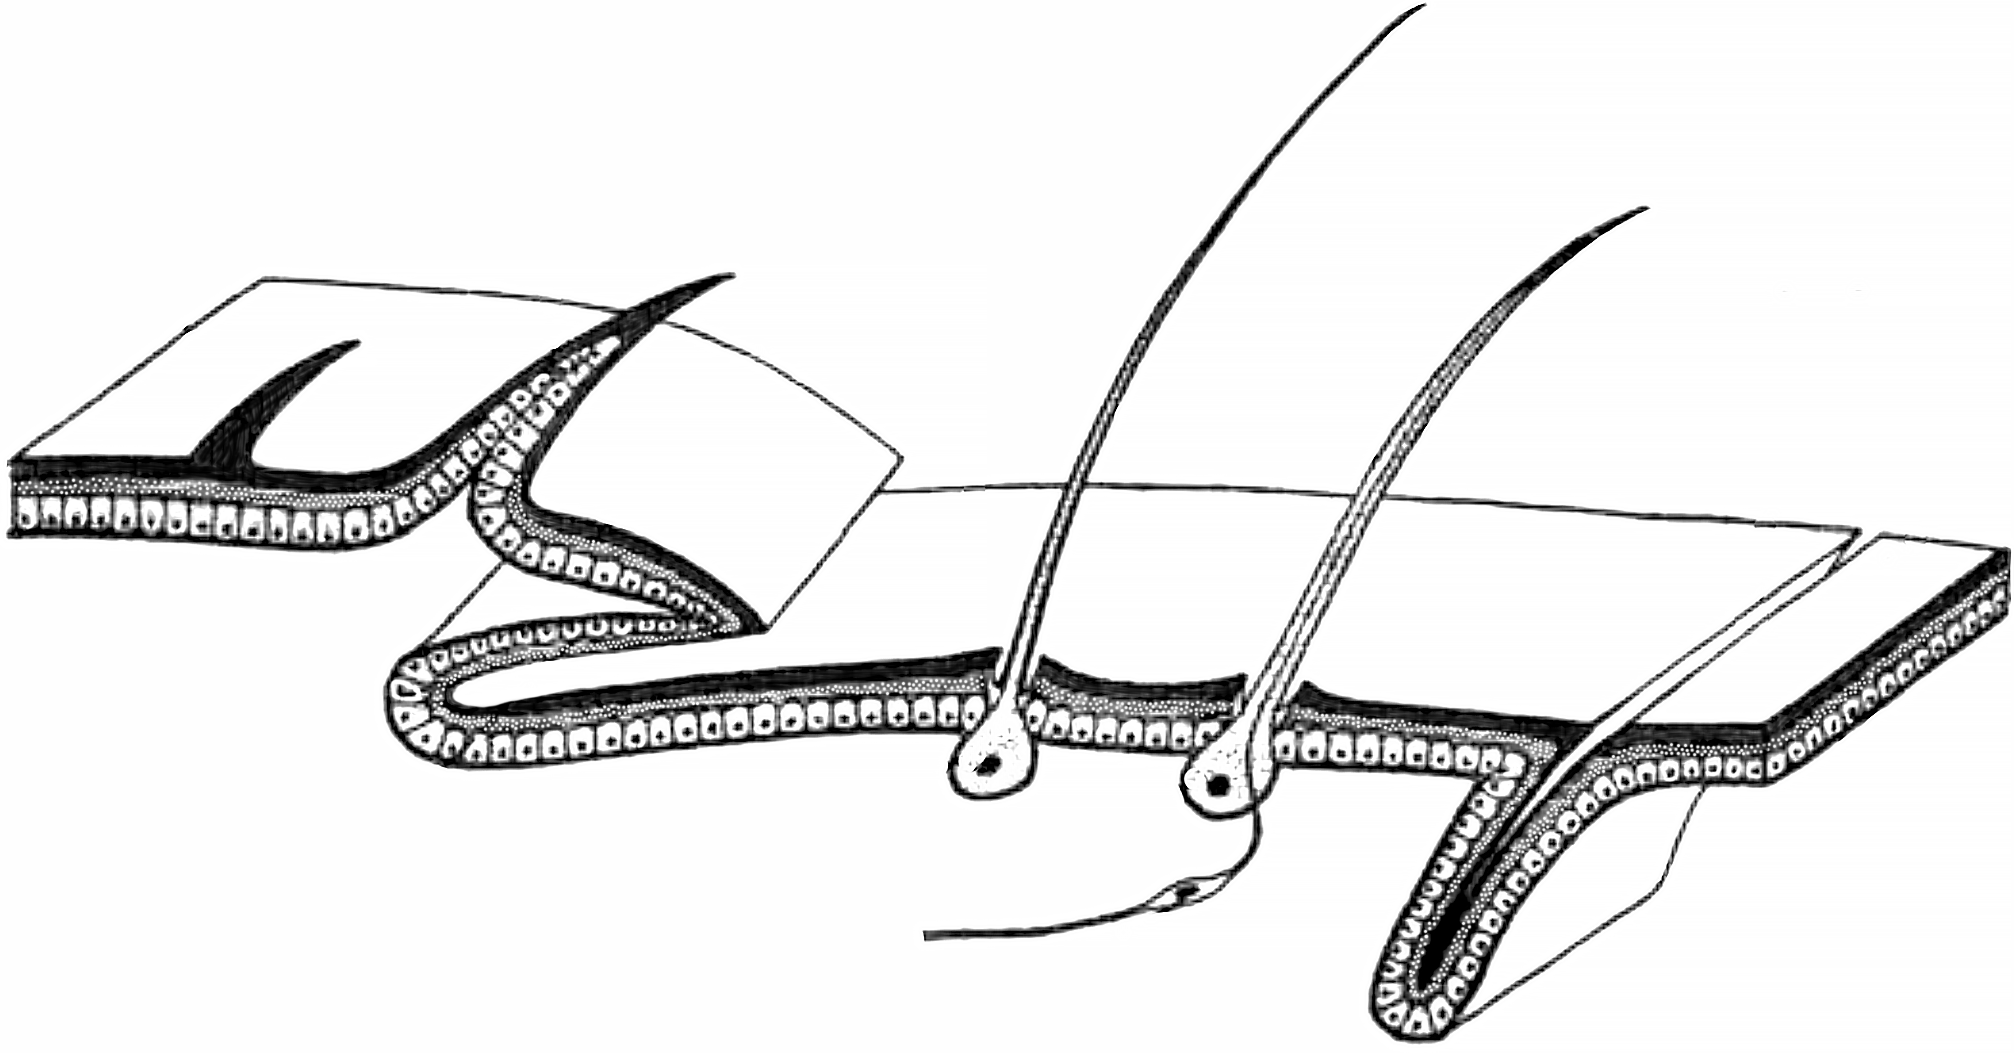
\includegraphics[width=0.7\textwidth]{morphology/cuticular}
  \caption{Features of insect cuticle \citep[redrawn and modified from][Fig. 43, a figure after illustrations by Snodgrass and Comstock]{metcalf1939destructive}}
  \label{fig:cuticular}
\end{figure}
\clearpage
\thispagestyle{empty}


\chapter[Early arthropods, fossils, and terrestrialization]{Early arthropods, fossils, \\ and terrestrialization}
\section{Introduction}
A major reason for the incredible diversity of Arthropoda is their successful colonization of terrestrial environments and their ability to adapt to the environmental extremes found there. We will discuss hypotheses and evidence concerning the emergence of arthropods from marine habitats. What did early arthropods look like, and what challenges did they face? How are fossils formed, and what kinds of information can we derive from them (and what \textit{can't} we get from them)? Where do we find fossils? 

\section{Taphonomy}
\latinword{Taphonomy} is the study of how organisms decay after dying, how they settle into positions that may result in fossilization, and how those fossils change chemically, geologically, \textit{etc}. over time. In this lab we have demonstrations that represent two elements of taphonomy: \latinword{decomposition}, the decay of a carcass, and \latinword{biostratinomy}, the processes that affect a carcass prior to deposition. The intention is to get you thinking about biases in the fossil record. The geologic elements of taphonomy, diagenesis for example, are beyond the scope of this class.

\subsection{Insects trapped in resin}
Amber is fossilized tree resin---\textit{i.e.}, the viscous compounds produced by plants, in response to damage. One can imagine that oozing, sticky goo from tree wounds would be a prime attractant for (some) insects. Many insects get trapped, and, if the conditions are right, their fates are preserved for us to see, millions of years later. We'll look at some real amber fossils, but first we'll try an experiment.

\begin{theo}
{}Jot down a few biases you would expect to see in amber fossils. Think about the insect morphology and natural history. Are there certain behaviors or structures that lend themselves to entrapment or escape? Why would an insect be attracted to resin? Or would they?\end{theo}\vspace{3mm}

\noindent{}We've provided several insect specimens and parts. Using your forceps, try sticking these specimens, one at a time, in a drop of Canada balsam. Does it stick?

\begin{theo}
{}What difference, if any, do you see in the way that specimens interact with this sticky substrate. Given these observations, what would you expect to see in the fossil record and why?\end{theo}\vspace{3mm}

\subsection{Insects decomposing}
Most non-amber fossils (compression fossils, concretions, ichnofossils, \textit{etc}.) are derived from insects that became trapped or otherwise interacted with aquatic and/or sedimentary environments. Several specimens have been placed in situations that simulate early taphonomy of these fossils. Take some time predict and observe the condition of each before answering the next question.\vspace{3mm}

\begin{theo}
{}Describe what you see in each jar. Based on their decomposition, what would you predict about the fossil record and potential biases?\end{theo}

\section{Fossil arthropods}
Our collection holds several arthropod fossils, each from a different \latinword{Lagerst\"atte}: 

\paragraph{Ichnofossil, unknown source (probably Carboniferous, $\sim$359--299 Mya)} This greenish, flat sedimentary rock has multiple track ways across it.

\paragraph{Old Port Formation, Shriver member (Early Devonian, $\sim$419--393 Mya)} These sedimentary rocks, which were collected in Huntingdon Co., Pennsylvania, are dark gray or orange-yellow in color, with molds and fossils of trilobites. These arthropods lived in the ocean, which covered much of Pennsylvania in the Devonian. Be sure to find the fossil that includes a trilobite's compound eye.

\paragraph{Creede Formation (Oligocene, $\sim$27 Mya)} You will see several grayish, flat rocks that have compression fossils in them, similar to figure \ref{fig:creedeFossil}. These insects lived in and around a shallow, high altitude lake in what is now Creede, CO. The lake was repeatedly filled with volcanic ash, from eruptions and from runoff \citep{berkeley}.

\begin{figure}[ht!]
  \centering
    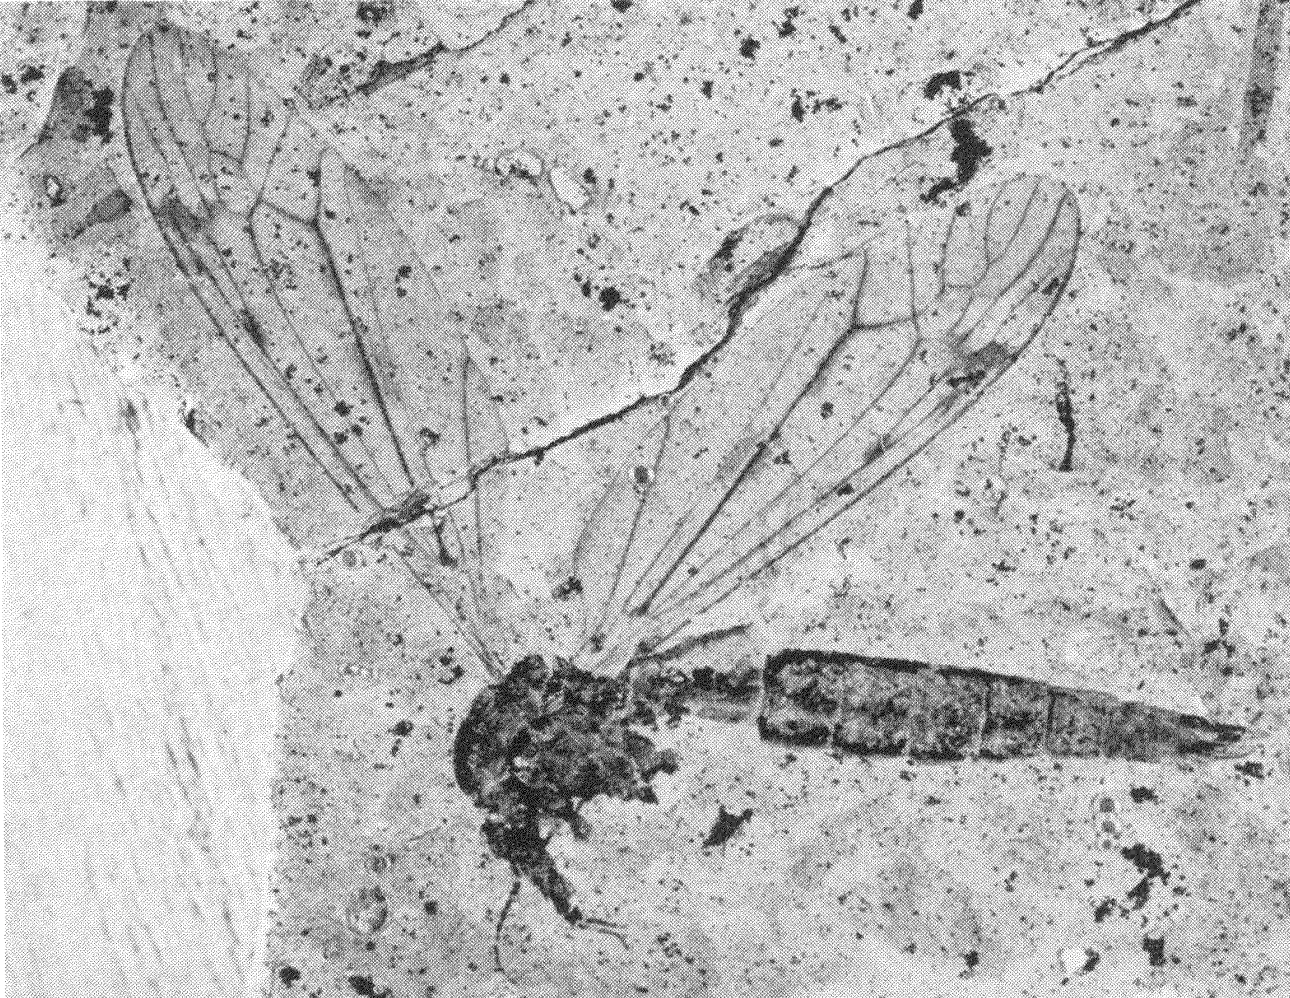
\includegraphics[width=0.35\textwidth]{creedeFossil}
  \caption{Crane fly, Creede Formation. \citep[][Fig. 1]{carpenter1938fossil}}
  \label{fig:creedeFossil}
\end{figure}

\paragraph{Dominican amber (Middle Miocene, 15--20 Mya)} We have a small collection of amber with insect inclusions. These insects lived in what is now the Dominican Republic. This amber is the fossilized resin from a leguminous tree, \textit{Hymenaea protera} (Fabaceae), now extinct \citep{IturraldeVinent1850}.

\paragraph{Barstow Formation (Early to Middle Miocene, 19.3--13.4 Mya)} These fossils are quite small and are mounted on slides. These insects are presumed to have lived in a series of saline-alkaline lakes that was repeatedly subjected to volcanic disturbance. Eruptions repeatedly killed the lakes' fauna and covered the carcasses with ash and calcium carbonate. The subsequent chemistry allowed silica to replace the integument and for the preservation of soft tissues \citep{PARK01042001}.

\begin{theo}
{}Spend some time with each type of fossil. Are they biased towards some particular life history or body part, as you hypothesized in section 1? Sketch a couple specimens in your lab notebook and label the parts. Which fossils offer the most information and why? How did the trilobite's compound eye get preserved? What can you infer from the trackways?\end{theo}

\section{Terrestrial adaptations}
We discussed the terrestrialization of Arthropoda and Earth's early history. Take a few minutes to remind yourself of the challenges faced by marine organisms as they moved onto land, before moving on to the next two demonstrations.

\subsection{Respiration}
In the morphology lab you learned about spiracles and tracheae, the primary mechanism through which most terrestrial hexapods respire. Think about how these structures are adapted for an environment that threatens desiccation. Now examine a decapod and a xiphosuran (horseshoe crab) and see if you can identify the structures associated with respiration. Can you find analogous structures on a terrestrial isopod, a scorpion, or a spider? What about an onychophoran?

\subsection{Integument}
Let's take a quick look at some other adaptions to terrestrial, and in this case very, very dry habitats. Death-feigning beetles (Tenebrionidae: \textit{Asbolus verrucosus} (LeConte, 1852)) live in the Sonoran Desert. Gently pick one up and look at it under the microscope.

\begin{theo}
{}Sketch the respiratory structures you can find in the decapod, the terrestrial isopod, the xiphosuran, and the scorpion. How do the terrestrial taxa remediate water loss? Can you see any relevant traits in the death-feigning beetle?\end{theo}

\section*{Test yourself}
Before moving on make sure you're comfortable with the following concepts. Could you write a couple sentences that explain each term? Can you provide examples?

\begin{enumerate} 
\item{\textit{Lagerst{\"a}tte}} 
\item{taphonomy}  
\item {stem \textit{vs}. crown group}
\end{enumerate}

\noindent{}Can you describe three types of fossils and how they occur? What factors influence preservation, and what environmental conditions result in well-preserved fossils? \citep[Hint: see][]{taphonomy2004}\vspace{3mm}

\noindent{Given what we know about insect bodies and biology, what biases would you expect to see in the fossil record and why?}\vspace{3mm}

\noindent{What can fossils tell us about insect evolution and biology?}\vspace{3mm}

\noindent{When did arthropods originate and in what environmental context? What about Insecta?}\vspace{3mm}

\noindent{We discussed the evolution of Arthropods through nine geologic periods, beginning with the Cambrian. Can you name these periods and describe in one to three sentences the relevance of each---environmental conditions (generally), types of insects present, and where to find fossils?}\vspace{3mm}

\noindent{What characteristics of the arthropod \textit{Bauplan} allowed these organisms to move into terrestrial environments? When and how many times (minimally) did this happen?

\clearpage
\thispagestyle{empty}


\chapter[Systematics, past and present]{Systematics, past and \\present}
\section{Introduction}
Systematists are charged with describing, naming, estimating evolutionary history, and classifying organisms. Here we cover the history of classification, so that you can understand the context of systematics today. \cite{grimaldi2005evolution} and \cite{EngelKristensen2013} together provide a thorough review of this history if you're interested in more details.

Here we remind ourselves of certain core concepts in evolution, which will facilitate our understanding of how Arthropoda radiated and evolved. We'll also discuss the kinds of data and analytical approaches (and even philosophies) we use to estimate evolutionary history (\textit{i.e}., phylogeny).

\section{History, concepts, and people to know}
We'll open this unit with a discussion and slideshow about the history of systematics, as it relates to arthropods, and a reintroduction to evolutionary concepts. Take notes and think about the following questions before moving on to lab-oriented exercises.

\subsection{Systematists}
If asked to describe the accomplishments of these people in 1--2 sentences could you do it? Could you arrange these figures chronologically?

\begin{enumerate} 
\item{Aristotle} 
\item{Charles Darwin}  
\item {Johann C. Fabricius}
\item {Willi Hennig}
\item Niels P. Kristensen
\item{Carolus Linn\ae{us}}  
\item{Maria Sibylla Merian}  
\end{enumerate}

\subsection{Concepts}
Think about the concepts and questions below. Could you write a couple sentences that explain each term? Can you provide examples? Cycle through the hands-on exercises and come back to this section later. 

\begin{enumerate} 
\item classification
\item nomenclature
\item phylogenetics 
\item{natural selection} 
\item{adaptation}  
\item{species}  
\item {adaptive radiation}
\item {monophyletic \textit{vs}. polyphyletic}  
\item {homology \textit{vs}. homoplasy}  
\item {ancestral/plesiomorphic \textit{vs}. derived/apomorphic}
\end{enumerate}

\noindent{}Can you draw a phylogeny and interpret its meaning? Why are these diagrams important? \cite{baum2008phylogenics} provide a helpful guide.\vspace{3mm}

\noindent{}Can you describe three technologies or tools that allowed for major leaps forward in insect taxonomy? (You can probably think of more than three.)\vspace{3mm}

\noindent{}We discussed three types of data that are typically used to estimate phylogenies: phenotype (including behavior), ecology, and molecules (DNA, proteins, \textit{etc}.) Can you briefly describe some advantages and limitations of each data type?\vspace{3mm}

\noindent{}Can you describe the differences between a phenetic and a cladistic approach to phylogeny? What is our current approach to character and phylogeny interpretation?\vspace{3mm}

\section{Classify your specimens}
As you learned earlier, the external features of an arthropod, \textit{i.e}., the phenotypes we can easily observe through a microscope, are the primary source of characters we use to diagnose arthropods and to hypothesize evolutionary relationships. The goal of this lab is to review the morphological concepts you learned in the last unit and then to develop \latinword{characters} (descriptions of phenotypic variation) that help you understand and communicate about Arthropoda. Take some time to sort your specimens into groups.\vspace{3mm}

\begin{theo} 
{}How many groups did you make, and what body parts provided the evidence or characters to justify your groups?\end{theo}

\subsection{Anatomy refresher}
(10--15 min) Look at your lab notebook, and review your answers to questions in the last chapter. Let's see if we can write formal definitions for some of the concepts we learned. Here is the typical structure of a \textit{genus differentia}: A \textit{species} is a \textit{genus} that \textless{}some description of how it differs from other species in that genus\textgreater{}. Here is an example: A microscope is a piece of equipment that allows one to see small things. ``Microscope'' is the species here, and it belongs in the broader class (the \textit{genus}) ``piece of equipment''. Microscope differs from other pieces of equipment by being the one that allows one to see small things (\textit{i.e}., this is the \textit{differentia}).\vspace{3mm}

\begin{theo} 
{}Can you generate a \textit{genus differentia} definition for this anatomical concept:\vspace{3mm}

A \latinword{head} is a \makebox[30 mm]{\hrulefill} that \hrulefill.\vspace{3mm} 

\noindent{}What about for \latinword{ocellus}, \latinword{antenna}, \latinword{pedicel}, \latinword{mandible}, \latinword{maxilla}, \latinword{leg}, \latinword{fore leg}, \latinword{wing}, \latinword{fore wing}, \latinword{mesothorax}?\vspace{3mm}

\noindent{}Note that this is how Linnaeus structured his species descriptions.
\end{theo}

\subsection{Character and matrix development}
(30 min) Think of a \latinword{character} as a relatively broad class of possible phenotypes for a body part. ``Flagellomere shape'', ``femur color'', and ``claw presence'' are three examples of characters. Character states are more specific versions of the character, and they're typically numbered arbitrarily from 0 to $\infty$:\vspace{3mm}

Flagellomere shape:	0=flagellum round, 1=flagellum square\vspace{3mm}

Femur color: 0=femur red, 1=femur orange, 2=femur black\vspace{3mm}

Claw presence: 0=present, 1=absent\vspace{3mm}

With this list of characters, and a list of the taxa you're examining, we can score a matrix:
\begin{table}[H]
\centering
\label{my-label}
\begin{tabular}{lccc}
                             & \multicolumn{1}{l}{flagellomere shape} & \multicolumn{1}{l}{femur color} & \multicolumn{1}{l}{claw presence} \\ \cline{2-4} 
\multicolumn{1}{l|}{insect A} & \multicolumn{1}{c|}{0}                 & \multicolumn{1}{c|}{0}          & \multicolumn{1}{c|}{1}            \\ \cline{2-4} 
\multicolumn{1}{l|}{insect B} & \multicolumn{1}{c|}{1}                 & \multicolumn{1}{c|}{2}          & \multicolumn{1}{c|}{1}            \\ \cline{2-4} 
\multicolumn{1}{l|}{insect C} & \multicolumn{1}{c|}{0}                 & \multicolumn{1}{c|}{1}          & \multicolumn{1}{c|}{0}            \\ \cline{2-4} 
\end{tabular}
\end{table}

\noindent{}We can compute across matrices like this using software that provides us with phylogenetic trees and software that generates diagnostic tools (\textit{e.g}., multi-entry keys).\vspace{3mm}

\begin{theo}[systematics3] 
{}Choose eight of your specimens, and see how many characters you can create for them. Mimic the descriptive style you see in the examples above, and score your taxa in a matrix. How do you account for homology?\end{theo}

\subsection{Dichotomous keys}
(30 min) Dichotomous keys are common diagnostic tools, and you will almost certainly use several in your efforts to determine specimens in your collection. They are composed from character sets, like the table you generated above and typically look like this (adapted from \cite[][page 151]{borror1989introduction}:\vspace{3mm}

\begin{adjustwidth}{1cm}{}
1. With well-developed wings (adults) \dotfill{} 2\\
1$'$. Wingless or with wings vestigial or rudimentary (nymphs, larvae, and some adults) \dotfill{} 30\vspace{3mm}

\noindent{}2(1). Wings membranous, not hardened or leathery \dotfill{} 3\\
2$'$. Front wings hardened or leathery, at least at base; hind wings, if present, usually membranous \dotfill{}24
\end{adjustwidth}\vspace{3mm}

\noindent{}Think of it almost as a series of if-then statements. If your specimen has well-developed wings then go to line 2. If those wings are membranous then go to line 3.\vspace{3mm}

\noindent{}Look through the keys provided on the workbench. See any patterns? Try running a few of your specimens through the key.\vspace{3mm}

\begin{theo} 
{}Write a dichotomous key using the characters you developed above. What kinds of characters would you use first, those that are easy to understand or those that separate the taxa into similarly-sized groups?\end{theo}\vspace{3mm}

\subsection{Thinking phylogenetically}
(30 min) Look at your list of characters and ask yourself how many provide evidence concerning the evolution of these organisms. Which states are ancestral and which ones are derived, and why? How many do you think are purely diagnostic, offering no usable information for understanding evolution?\vspace{3mm}

\begin{theo}[systematics5] 
{}Draw a phylogenetic tree that represents your hypothesis for the evolutionary history of your specimens. Your instructors will demonstrate how to do this on the board. Map your character states on the tree. Do your data support your tree? Can you see evidence of convergent evolution?\end{theo}

\subsection{A few words about taxonomic ranks}
In many cases, one can learn a lot about zoological names just by looking at the endings. Linnean classification is organized hierarchically into \latinword{ranks}, which you might remember from biology class: kingdom, phylum, class, order, family, genus, and species. For the honey bee, the nested classification looks like this:\vspace{3mm}

Animalia $\leftarrow$ Arthropoda $\leftarrow$ Insecta $\leftarrow$ Hymenoptera $\leftarrow$ Apidae $\leftarrow$ \textit{Apis} $\leftarrow$ \textit{mellifera}\vspace{3mm}

\noindent{}Note that genus and species are always in a different font style, for example \textit{italics} or \underline{underlined}. When referencing a species one usually include both genus and species, plus the taxon's author and the year it was published. For the honey bee, the proper reference is \textit{Apis mellifera} Linnaeus, 1758. When the species name has been transferred to another genus since its original description, the author and year are put in parentheses. The black carpenter ant, for example was originally described by De Geer in 1773 as \textit{Formica pensylvanica}. The species was later transferred to \textit{Camponotus} and is now referred to as \textit{Camponotus pennsylvanicus} (De Geer, 1773).\vspace{3mm}

\noindent{}As our understanding and our naming of species has increased, so has the number of ranks: ... order, suborder, infraorder, superfamily, family, subfamily, tribe, subtribe, genus, subgenus, and so on. Some of these ranks (\textit{i.e.}, ``family group'' ranks) have suffixes that indicate their rank. For example, -oidea always refers to superfamily, -idae to family, -inae to subfamily, -ini to tribe, and -ina to subtribe.

\begin{theo}[ranks] 
{}Some taxonomists describe ranks as arbitrary and even burdensome, while others see them as critically useful. Entomologists tend to be in the latter camp, and yet the family-level classification in many orders remains highly unstable (as you will see!). Should we adhere to a rigid system of ranks? \end{theo}

\subsection{Solving nomenclatural problems}
We'll discuss the \cite{iczn} and its Code, portions of which are in the appendix of this handout. Read the following descriptions of nomenclatural problems, and see if you can find solutions in the pieces of the Code given to you in this handout (see Appendix I).\vspace{3mm}

\begin{theo}[systematics6] 
{}(1) Linn\ae{}us described the honey bee in 1758, naming it \textit{Apis mellifera}. Joe Schmoe insists on calling these insects \textit{Honeyus beeus}, however, because he found this name in an even older volume (1725), by another author. Joe thinks \textit{Honeyus beeus} should have priority, as spelled out in Article 23. What is the correct name? Which article resolves this conundrum?\vspace{3mm}

\noindent{}(2) Jane Doe tries to publish a new species name with a modern twist---a crane fly named \textit{Tipula p0k3m0norum} Doe, 2022. The peer review process informs her that this is not possible. Which article do her peers reference in their critique and why?\vspace{3mm}

\noindent{}(3) Frustrated with the high expense and slow rate of scientific publication (and the constant rejection of manuscripts by his peers), Randy Bobandy decides to self-publish all new species. He prints his manuscripts in his mom's basement, avoids peer-review, and mails them to several local libraries to be archived. Are these new names available? Why or why not?
\end{theo}

\section{Specimen data and accesibility}
The next set of exercises introduce you to some basic \latinword{biodiversity informatics}. You've started collecting and sorting insects, undoubtedly from numerous localities. You've also made specimen preparations and labeled each one according to collection best practices. As part of this process you've also established a database of specimens in your collection: a spreadsheet with columns for locality, collector, identifier, \textit{etc}. You should be using the prescribed spreadsheet format for this class, but Appendix II describes how to make non-standard spreadsheets accessible.\vspace{3mm}

\noindent{}We'll talk a bit about biodiversity data standards and tools and other resources that facilitate data sharing. 

\section*{Glossary}
We'll be using terms you may not be familiar with. Some of these concepts are provided below, and we'll go over them together. If you have a new one to add raise your hand!
\begin{enumerate} 
\item {Darwin Core}
\item {GBIF}
\item {metadata}
\item{TDWG} 
\end{enumerate}

\section*{Your data}
Take a look at this label, which probably looks similar to the labels you've created for your specimens:\vspace{3mm}

\begin{labelfontsmall}
\tiny
\noindent{USA: PA: Centre County: \\ Pine Grove Mills, 40.730, \\ -77.884, $\pm$250m 15.iv.2023 \\ A.R. Deans, sifted litter}
\end{labelfontsmall}
\normalsize\vspace{5mm}

\begin{theo}[systematics7] 
{}What kinds of data do you see represented? How many kinds are there? List them.\vspace{3mm}

\noindent{}If you had these data from millions of specimens---all 35+ million insects in the Smithsonian Institution, for example---what kinds of hypotheses could you test? See if you can think of three example research questions.
\end{theo}

\section*{Biodiversity data in research}
Biodiversity science is incredibly rich, with respect to the array of research questions and the data types that can be applied to them. We'll discuss a few examples of research that relies on collections data. As we talk, think about the minimum data required for these kinds of questions.

\section*{Biodiversity data standards}
How can we aggregate data from hundreds (or thousands!) of natural history collections to test your hypotheses? You can imagine that natural history collections across the world might each have a different approach to recording data; for example Museum A might record dates of collection as ``2023-08-31", while Museum B uses ``31-08-2023'' and Museum C records dates as ``31.viii.2023''.\vspace{3mm}

\noindent{}Fortunately there are established biodiversity data standards and tools that facilitate sharing. We'll look at those developed by TDWG, especially the Darwin Core and associated resources. Your homework: Open a Web browser and navigate to \url{https://dwc.tdwg.org/terms/}. This massive list almost definitely includes data types you use, along with dozens more that may or may not be relevant to your collection.\vspace{3mm}

\noindent{}Find the following terms and read their definitions: \latinword{catalogNumber}, \latinword{recordedBy}, \\\latinword{eventDate}, \latinword{samplingProtocol}, \latinword{stateProvince} and \latinword{locality}, \latinword{decimalLatitude}, \\\latinword{decimalLongitude},  \latinword{scientificName}. Do any of these sound familiar?\vspace{3mm}

\section*{More thoughts on biodiversity data}
Now that you have an idea of how to create a set of files that contribute to the greater scientific enterprise it's time to think about how to extend and enrich your data sets. We'll discuss some of these issues as a group.
\begin{itemize}
\item Many journals (\textit{e.g.}, PLoS) and granting agencies want information about specimen provenance and collecting permits. How would you incorporate that into your spreadsheet or archive?
\item All of your specimens will be deposited at the Frost Entomological Museum. How do we specify that in your file?
\item Do any of you have images or videos? How do we associate them with specimen records?
\item How do we associate specimens, for example a parasitoid and its host? 
\item How do we account for a range of dates, as we might see with a Malaise trap?
\item How to explain our approach to georeferencing (\textit{i.e.}, finding a latitude and longitude for each specimen)? Do you know what geodetic datum means?
\item Can biodiversity data be copyrighted?
\end{itemize}

\section*{\textit{ProTip}\texttrademark}
GBIF provides structured spreadsheets as Microsoft Excel files: 
\url{https://ipt.gbif.org/manual/en/ipt/latest/occurrence-data}. These files can be imported through any of the myriad Integrated Publishing Toolkit (IPT) instances.

\clearpage

\section*{Appendix. Portions of the International Code of Zoological Nomenclature}

The following text was copied from the ICZN online edition (\url{https://www.iczn.org/}). It has been simplified for the exercises in this handout. Not all articles are included.

\subsection*{Article 3. Starting point.} 

The date 1 January 1758 is arbitrarily fixed in this Code as the date of the starting point of zoological nomenclature.

\subsection*{Article 5. Principle of Binominal Nomenclature.}

\paragraph*{5.1. Names of species.} The scientific name of a species, and not of a taxon of any other rank, is a combination of two names (a binomen), the first being the generic name and the second being the specific name. The generic name must begin with an upper-case letter and the specific name must begin with a lower-case letter.

\subsection*{Article 8. What constitutes published work.}
A work is to be regarded as published for the purposes of zoological nomenclature if it complies with the requirements of this Article and is not excluded by the provisions of Article 9.

\paragraph*{8.1. Criteria to be met.} A work must satisfy the following criteria:

\begin{itemize}
    \item \textbf{8.1.1.} it must be issued for the purpose of providing a public and permanent scientific record,
    \item \textbf{8.1.2.} it must be obtainable, when first issued, free of charge or by purchase, and
    \item \textbf{8.1.3.} it must have been produced in an edition containing simultaneously obtainable copies by a method that assures
    \begin{itemize}
        \item \textbf{8.1.3.1.} numerous identical and durable copies, or
        \item \textbf{8.1.3.2.} widely accessible electronic copies with fixed content and layout.
    \end{itemize}
\end{itemize}


\subsection*{Article 9. What does not constitute published work.}
Notwithstanding the provisions of Article 8, none of the following constitutes published work within the meaning of the Code:

\paragraph*{9.1.} after 1930 handwriting reproduced in facsimile by any process;

\paragraph*{9.2.} after 1985, works produced by hectographing or mimeographing;

\paragraph*{9.3.} before 1986 and after 2012, works issued on optical discs;

\paragraph*{9.4.} photographs as such;

\paragraph*{9.5.} proof sheets;

\paragraph*{9.6.} microfilms;

\paragraph*{9.7.} acoustic records made by any method;

\paragraph*{9.8.} labels of specimens;

\paragraph*{9.9.} preliminary versions of works accessible electronically in advance of publication (see Article
21.8.3);

\paragraph*{9.10.} materials issued primarily to participants at meetings (e.g. symposia, colloquia, congresses, or workshops), including abstracts and texts of presentations or posters;

\paragraph*{9.11.} text or illustrations distributed by means of electronic signals (e.g. via the Internet), except those fulfilling the requirements of Articles 8.1 and 8.5.

\paragraph*{9.12.} facsimiles or reproductions obtained on demand of an unpublished work [Art. 8], even if previously deposited in a library or other archive.

\subsection*{Article 11. Requirements [for the availability of a name].}
To be available, a name or, where relevant, a nomenclatural act must satisfy the following provisions:

\paragraph*{11.1. Publication.} The name or nomenclatural act must have been published, in the meaning of Article 8, after 1757.

\paragraph*{11.2. Mandatory use of Latin alphabet.} A scientific name must, when first published, have been spelled only in the 26 letters of the Latin alphabet (taken to include the letters j, k, w and y); the presence in a name when first published of diacritic and other marks, apostrophes or ligatures, or a hyphen, or a numeral in a compound species-group name, does not render the name unavailable (for corrections, see Articles 27 and 32.5.2).

\paragraph*{11.3. Derivation.} Providing it meets the requirements of this Chapter, a name may be a word in or derived from Latin, Greek or any other language (even one with no alphabet), or be formed from such a word. It may be an arbitrary combination of letters providing this is formed to be used as a word.

\subsection*{Article 14. Anonymous authorship of names and nomenclatural acts.}
A new name or nomenclatural act published after 1950 with anonymous authorship is not thereby made available.

\subsection*{Article 18. Inappropriate and tautonymous names.}
The availability of a name is not affected by inappropriateness or tautonymy.

\subsection*{Article 23. Principle of Priority.}

\paragraph*{23.1. Statement of the Principle of Priority.} The valid name of a taxon is the oldest available name applied to it, unless that name has been invalidated or another name is given precedence by any provision of the Code or by any ruling of the Commission. For this reason priority applies to the validity of synonyms, to the relative precedence of homonyms, the correctness or otherwise of spellings, and to the validity of nomenclatural acts (such as acts taken under the Principle of the First Reviser and the fixation of name-bearing types).

\subsection*{Article 61. Principle of Typification.}

\paragraph*{61.1. Statement of the Principle of Typification.} Each nominal taxon in the family, genus or species groups has actually or potentially a name-bearing type. The fixation of the name-bearing type of a nominal taxon provides the objective standard of reference for the application of the name it bears.

\subsection*{Article 76. Type locality.}

\paragraph*{76.1. Definition.} The type locality of a nominal species-group taxon is the geographical (and, where relevant, stratigraphical) place of capture, collection or observation of the name-bearing type; if there are syntypes and no lectotype has been designated, the type locality encompasses the localities of all of them.

\subsection*{Article 78. Powers and duties of the Commission.}

\paragraph*{78.1. Plenary Power.} The Commission is empowered, by a resolution of the IX International Congress of Zoology (1913) and ratified in subsequent Codes by its successors, under conditions specified in Article 81 to suspend the application in a particular case of any provision of the Code except those in the present and next succeeding Chapter. The course to be followed is decided by the Commission under this plenary power and its ruling is published in an Opinion [Art. 80.2].
\thispagestyle{empty}

\chapter{Non-hexapod Arthropoda}
\section{Introduction}
Here we learn about major non-hexapod arthropod lineages---\textbf{Chelicerata} (spiders, mites, scorpions, and their relatives), \textbf{Myriapoda} (centipedes, millipedes, and their relatives), and some non-hexapod \textbf{Pancrustacea} (pillbugs, brine shrimp, and their relatives)---including their natural histories and hypotheses of their evolutionary history. We'll also look at the likely sister to Arthropoda: \textbf{Onychophora} (velvet worms).

You should have a firm grasp of arthropod anatomy now. Before we start, revisit our discussion of the phenotypes that make an organism an arthropod. Now consider their diversity relative to other metazoans: vertebrates, annelids, nematodes, \textit{etc}. What phenotypes would you consider \latinword{key innovations} for Arthropoda? Why is Arthropoda orders of magnitude more diverse than its sister lineage? As you examine the specimens in the hands-on portion of this unit think about how the traits you observe inform us of the evolutionary history of these organisms.

\section{Onychophora (velvet worms)}\index{Onychophora}
\noindent{}\textit{Diagnostic characters:} Segmented and relatively soft body, with a single pair of antennae and serially homologous legs. Legs unsegmented. Tagmata not obvious.\vspace{3mm}

\noindent{}\textit{Natural history:} Velvet worms are predators of other invertebrates, usually subduing prey with a glue-like mucous that is excreted with force from glands near the mouth. They are quite susceptible to desiccation and so are usually found in humid habitats. There are approximately 200 species, which can found throughout the Neotropics and in pockets throughout the rest of the world. There is a rich fossil record of onychophoran-like organisms (``Lobopodia'') from marine environments, but there are no extant marine species.\vspace{3mm}

\begin{theo}[Onychophora]
{}Can you see any shared, derived characters (figures \ref{fig:onych},\ref{fig:onychLeg}) between onychophorans and arthropods? What traits indicate that these creatures are  \textit{not} Arthropoda?
\end{theo}

\begin{figure}[ht!]
  \centering
    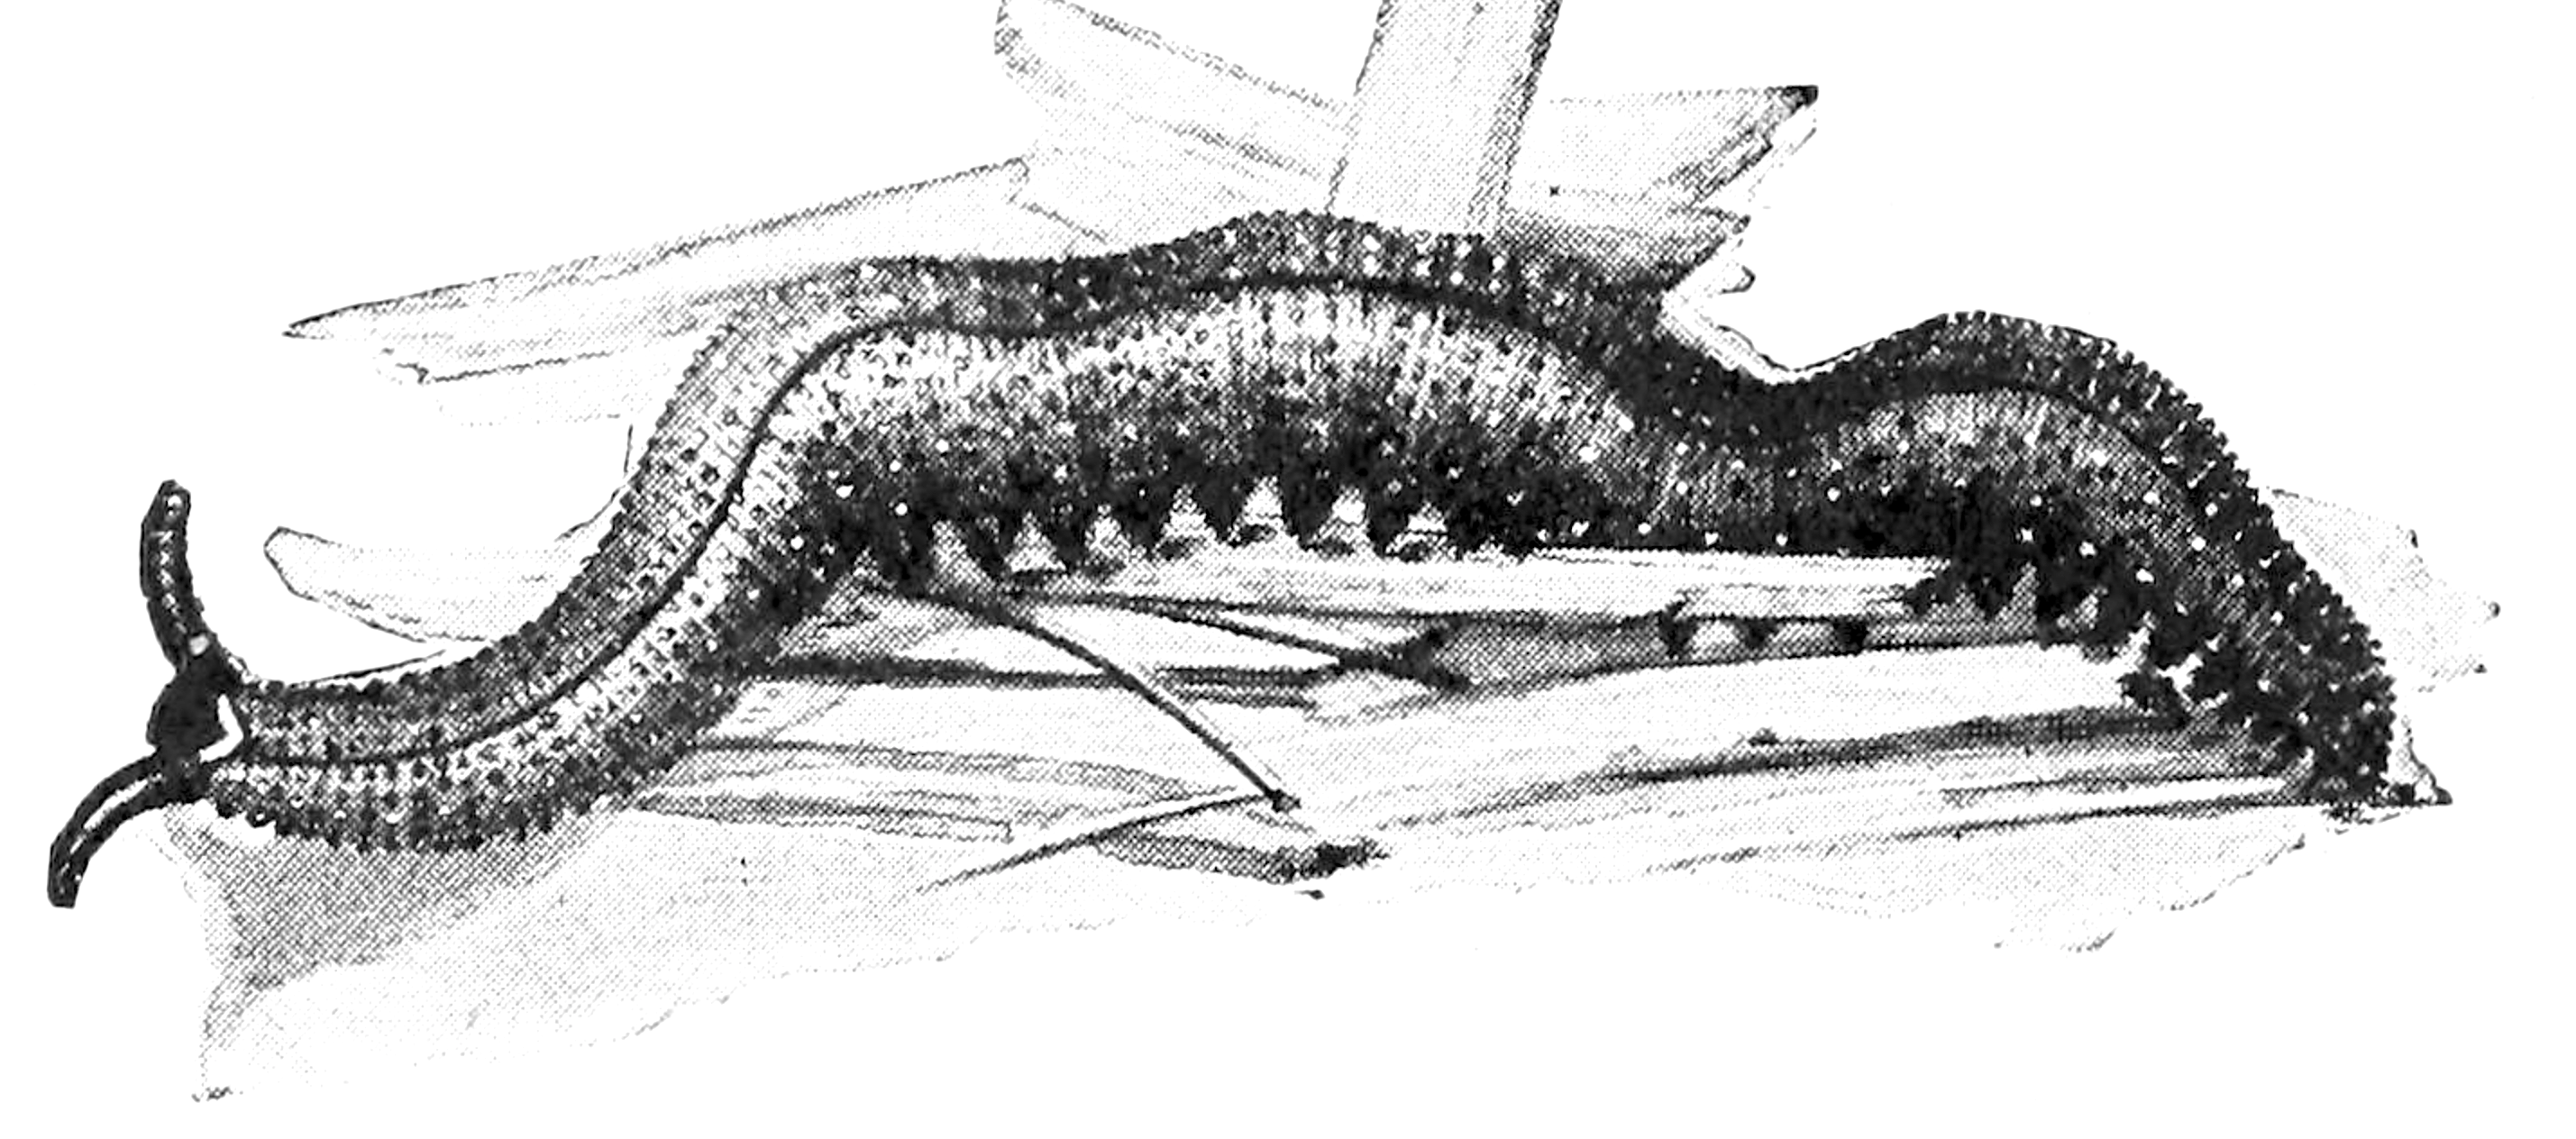
\includegraphics[width=0.85\textwidth]{nonhexapod/onychophora}
  \caption{Onychophora habitus \citep[][Fig. 81]{bhlitem40112britmus}}
  \label{fig:onych}
\end{figure}

\begin{figure}[ht!]
  \centering
    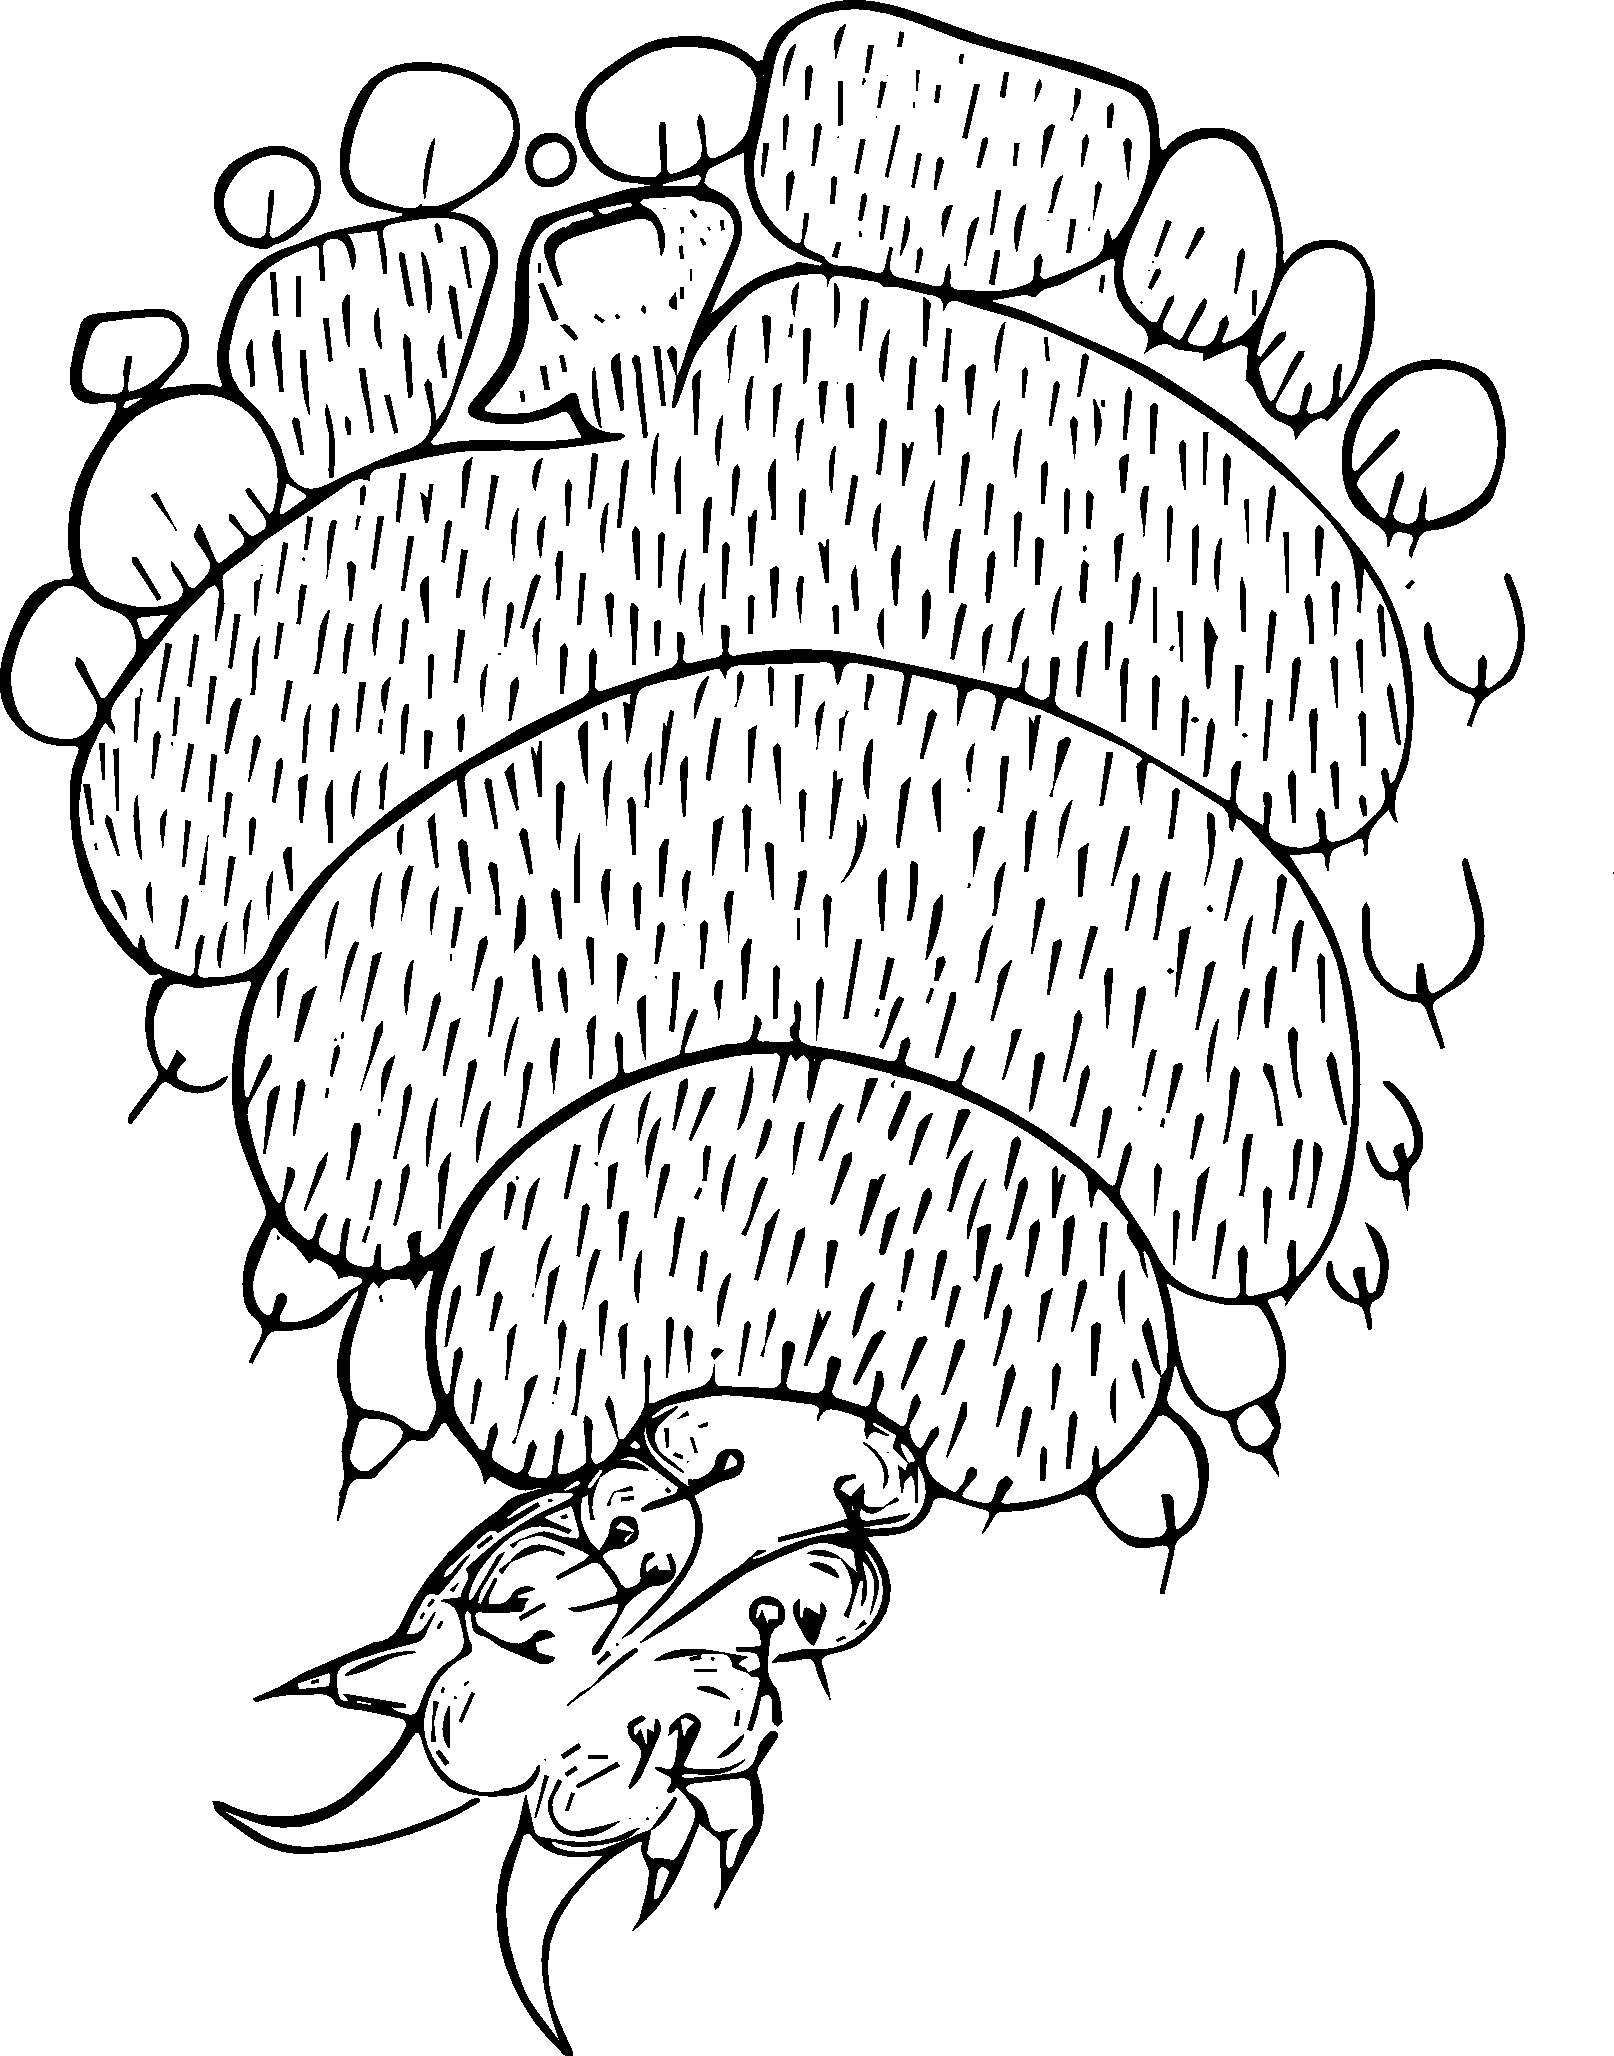
\includegraphics[width=0.22\textwidth]{nonhexapod/onychLeg}
  \caption{Onychophora leg \citep[][Fig. 6]{bhlpart201070OnychLeg}}
  \label{fig:onychLeg}
\end{figure}

\section{Chelicerata}\index{Chelicerata}
We are now looking at true arthropods, beginning with Chelicerata. Members of this lineage share the following characters: 
\begin{itemize}
\item antennae absent (though anteriormost pair of legs often antenniform)
\item 6 pairs of \latinword{uniramous} appendages: chelicerae (mouthparts) + pedipalps + 4 pairs of legs
\item 2 tagmata: \latinword{prosoma} (cephalothorax) and \latinword{opisthosoma} (abdomen)
\end{itemize}

\subsection{Xiphosura (horseshoe crabs)}\index{Xiphosura}
\noindent{}\textit{Diagnostic characters:} Prosoma covered by large carapace that has two compound eyes; appendages, including chelicerae, relatively uniform in morphology; book gill present; long spine (telson) present on posterior margin of opithosoma.\vspace{3mm}

\noindent{}\textit{Natural History:} Approximately four extant species known worldwide, all of which are marine. Their diet includes molluscs and other marine invertebrates, which they masticate with spines on the four anteriormost pairs of legs (gnathobase).\vspace{5mm}

\begin{theo}
{}Recent phylogenies reveal that Xiphosura is deeply embedded \textit{within} Arachnida \citep[\textit{e.g}.,][]{d13110568}. Do you see evidence that these arthropods are related to other Arachnida? What does this mean with respect to terrestrialization in Chelicerata?
\end{theo}

\begin{figure}[ht!]
  \centering
    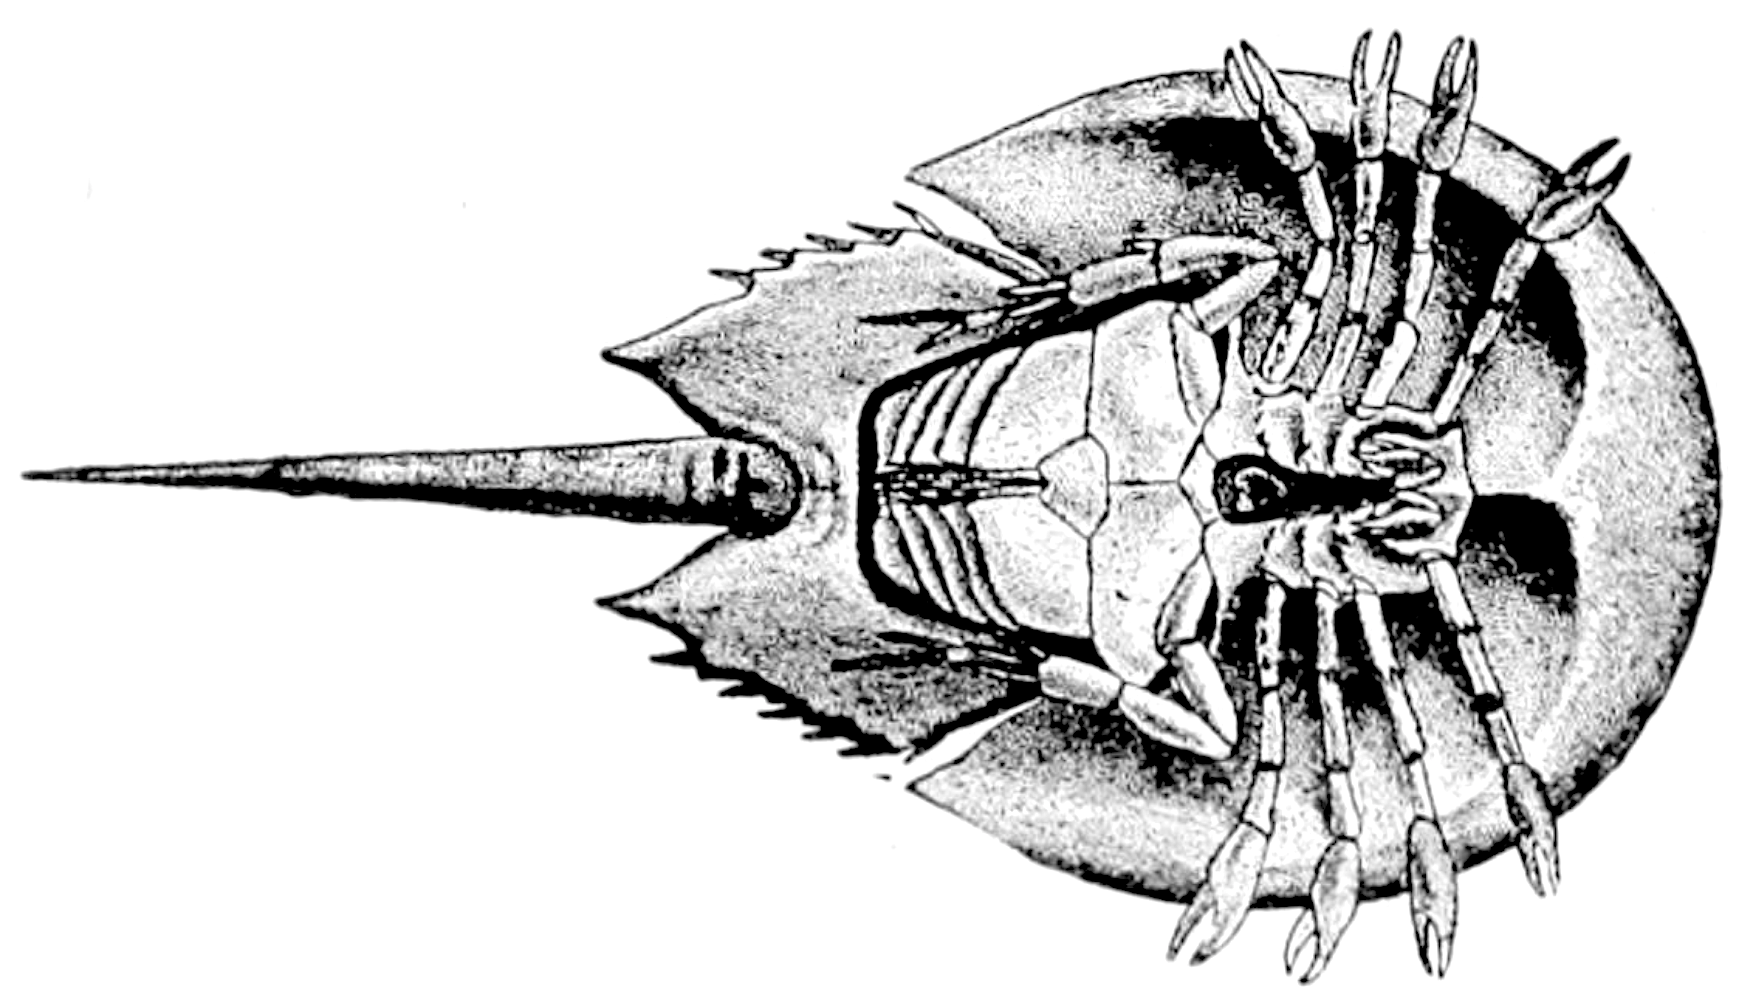
\includegraphics[width=0.7\textwidth]{nonhexapod/xiphosura}
  \caption{Xiphosura \citep[][Fig. 9]{bhlitem21199comstock}}.
  \label{fig:xipho}
\end{figure}
%https://www.biodiversitylibrary.org/page/2822779

\noindent{}The most diverse group of chelicerates is \textbf{Arachnida}, which includes all the terrestrial species of Chelicerata. We will examine specimens of the arachnid taxa listed below. Can you see the diagnostic characters clearly? If you saw any of these specimens in a lab practical could you name it (with correct spelling), describe a diagnostic feature, and/or describe its natural history?

\subsection{Araneae (spiders)}\index{Araneae}
\noindent{}\textit{Diagnostic characters:} Chelicerae fang-like (figure \ref{fig:fang}); anteriormost pair of legs not antenniform; pedipalps not chelate, rarely stouter than legs; opisthosoma not obviously segmented (except rarely); opisthosoma attached to prosoma via narrow constriction (figure \ref{fig:spider}); spinnerets present posteroventrally on opisthosoma, but no tail-like structure (telson).\vspace{3mm}

\noindent{}\textit{Natural History:} Incredibly diverse taxon, with more than 50,000 described species found worldwide and in almost every habitat. These arthropods are well known for their use of silk to form webs, tunnels, ``parachutes'', and other contraptions. They are all predators, although some will supplement their diets with pollen or other plant products.\vspace{3mm}

\begin{theo}[Araneae]
{}Find three spiders that look very different from each other, \textit{e.g.}, a tarantula, a jumping spider, and an orb weaver or cellar spider. Examine and sketch their eye patterns. Are they different? Find three males of different species and examine and sketch their pedipalps. Can you homologize their parts?\vspace{3mm}

\noindent{}Compare the chelicerae of a tarantula and an orb weaver or jumping spider. See any differences? Now compare the ventral habitus of their opisthosomata.\vspace{3mm}

\noindent{}Why do spiders have a constricted ``waist'', a trait not generally seen in other chelicerates?
\end{theo}

\begin{figure}[ht!]
    \centering
    \begin{subfigure}[ht!]{0.2\textwidth}
        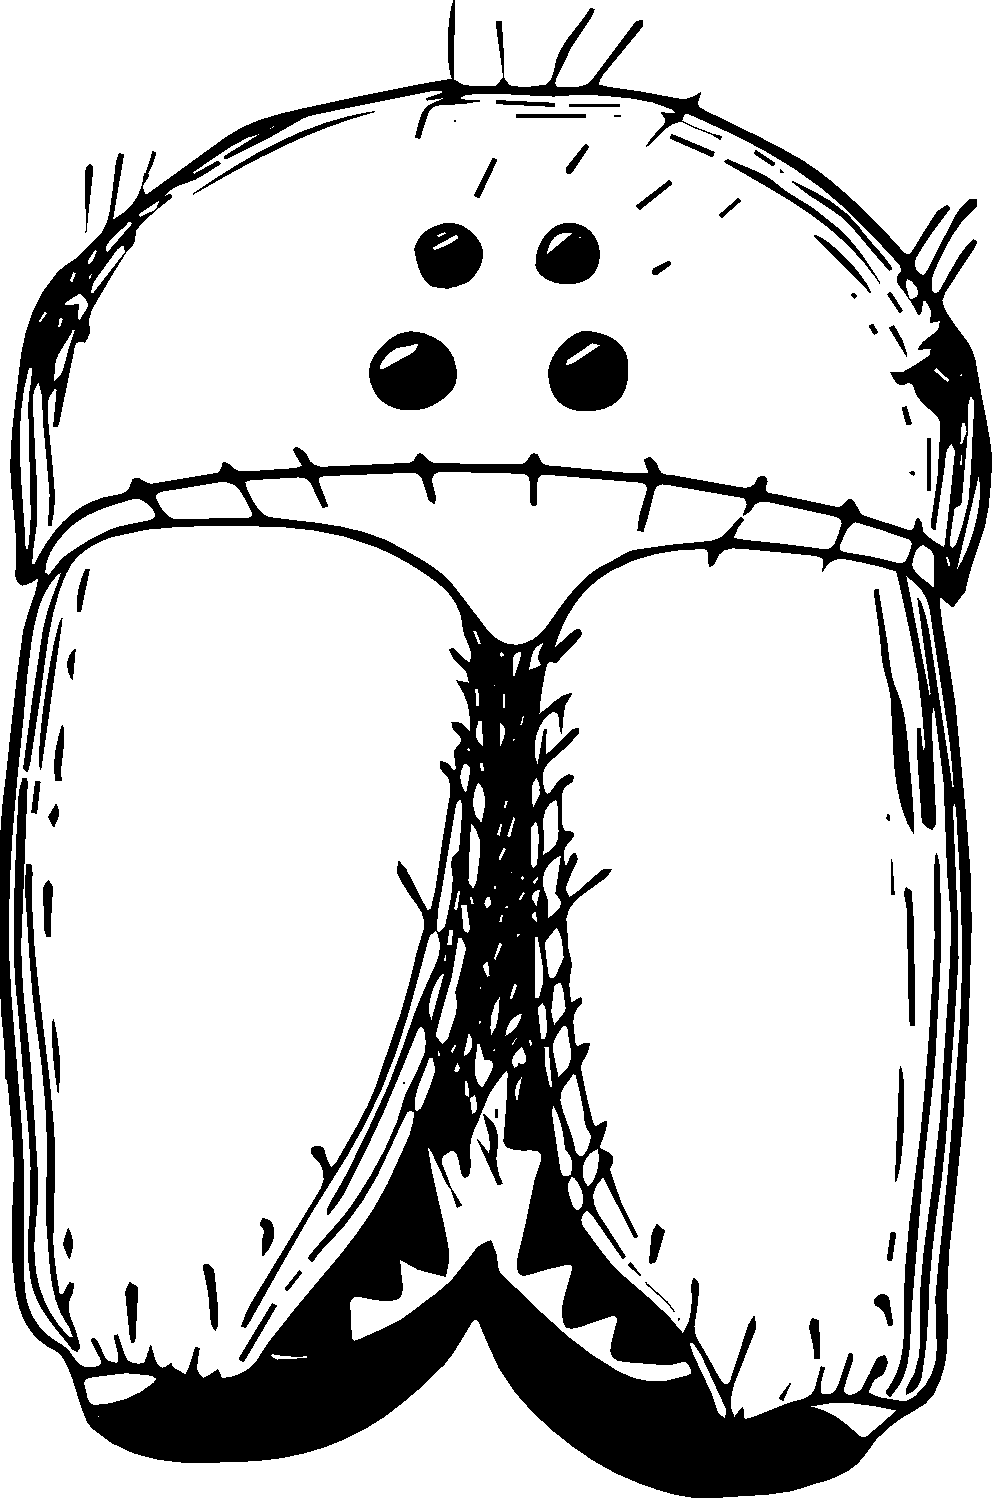
\includegraphics[width=\textwidth]{nonhexapod/spider78}
        \caption{}
        \label{fig:fang}
    \end{subfigure}
    \hfill
    \begin{subfigure}[ht!]{0.7\textwidth}
        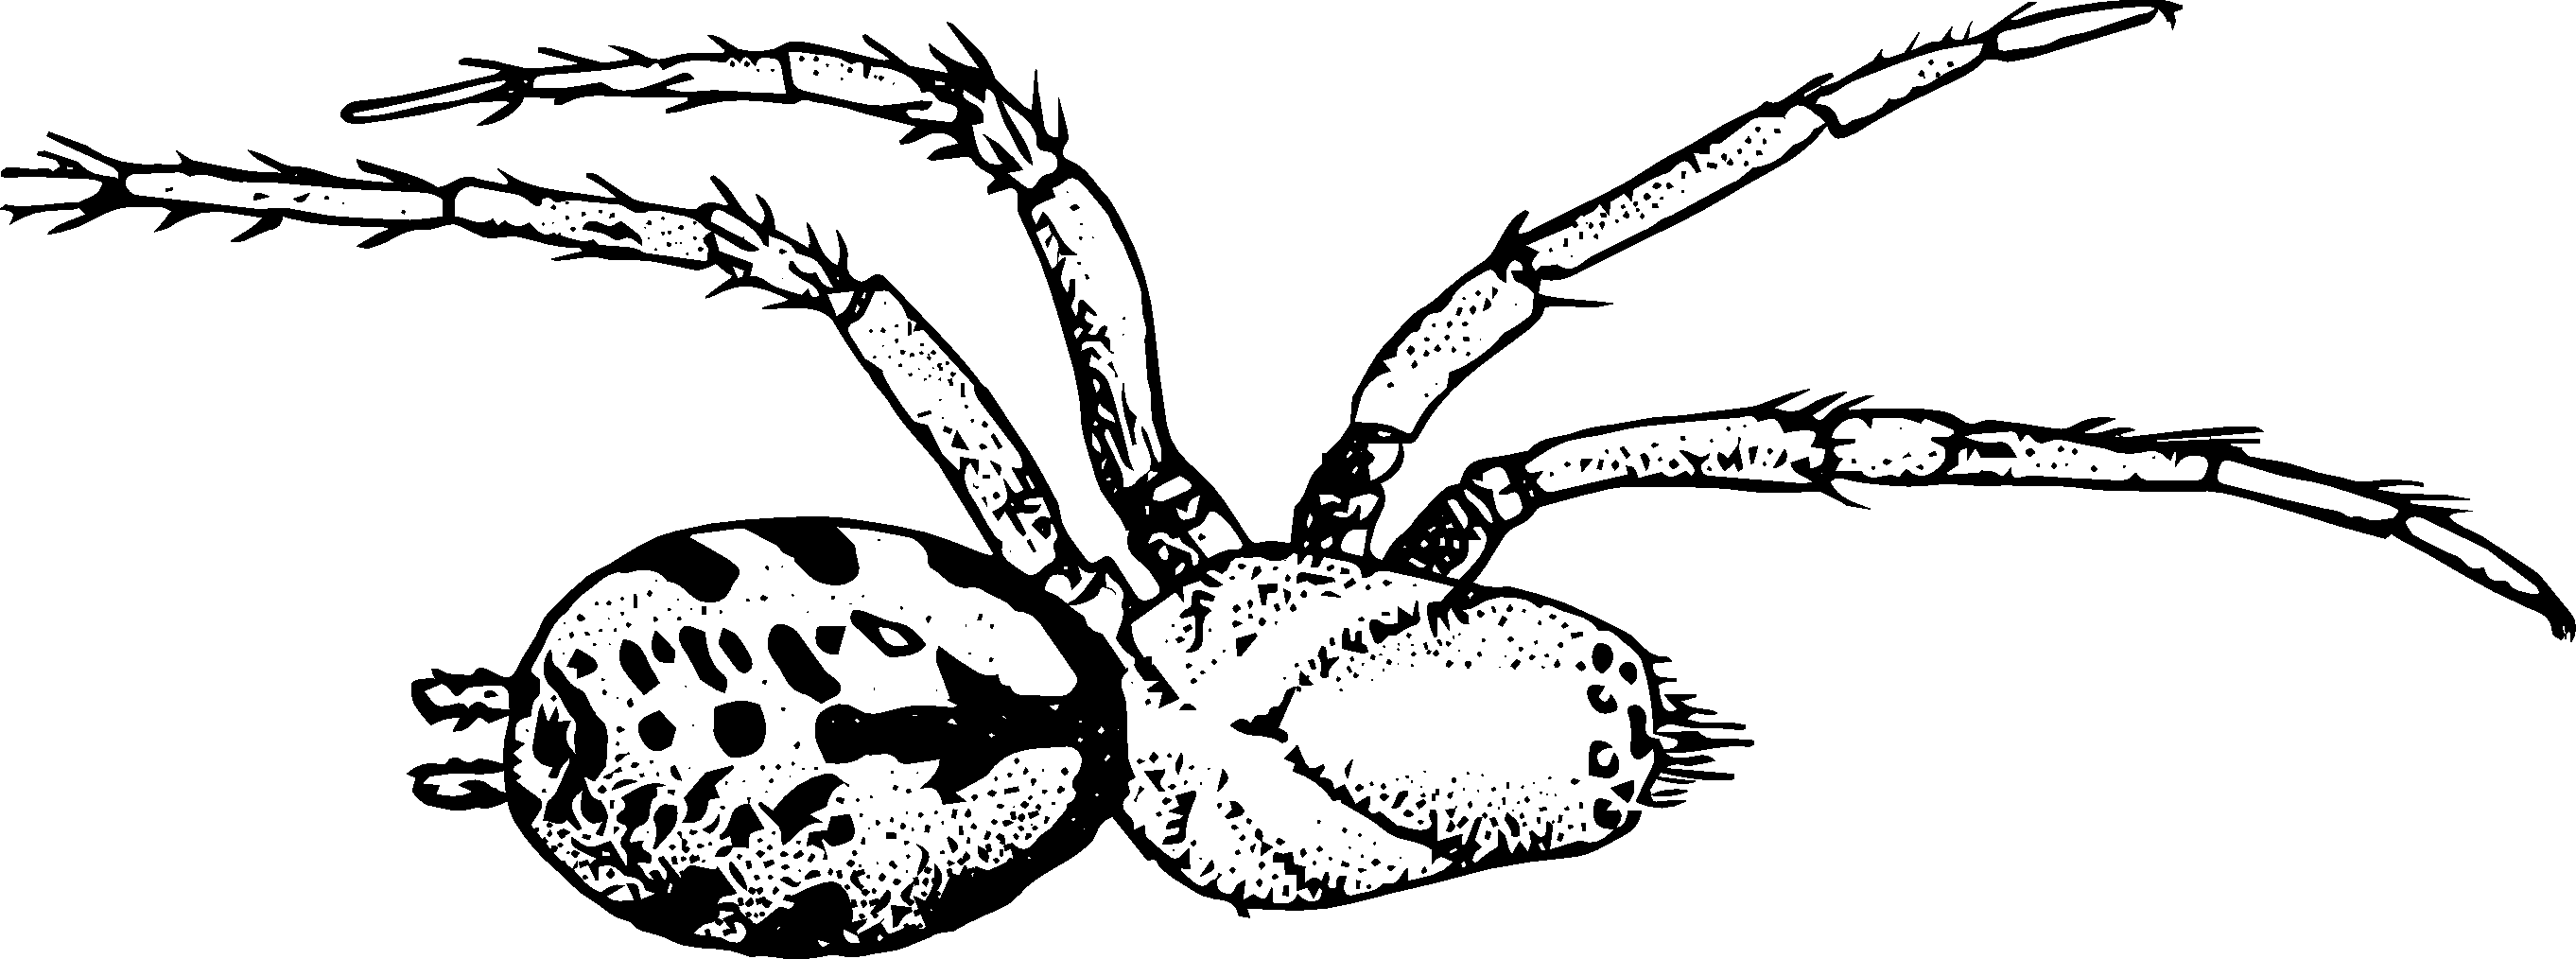
\includegraphics[width=\textwidth]{nonhexapod/spider314a}
        \caption{}
        \label{fig:spider}
    \end{subfigure}
    \caption{Spiders (Araneae). \textbf{(a)} Head in anterior view \citep[][Fig. 78]{bhlitem21199comstock}; \textbf{(b)} dorsal habitus \citep[][Fig. 314a]{bhlitem21199comstock}}\label{fig:spiders}
\end{figure}

\subsection{Acari (Acarina, mites, ticks)}\index{Acari}
\noindent{}\textit{Diagnostic characters:} Opisthosoma not segmented (See figure \ref{fig:mites}); opisthosoma broadly joined to prosoma, no tail-like structure (telson); young instars with 3 pairs of legs, adults with 4; pedipalps not chelate, not thicker than legs; mouthparts usually project anteriorly, chelicerae not chelate; usually very small (0.08--10 mm body length).\vspace{3mm}

\noindent{}\textit{Natural History:} Another incredibly diverse taxon, with more than 44,000 described species found worldwide. It is difficult to generalize their natural history, as there are species that feed as predators, herbivores, detritivores, fungivores, and parasites, and they live in just about every habitat imaginable. Recently people have started treating these arthropods as two superorders: Acariformes (mites, including eyelash mites and those that cause mange) and Parasitiformes (ticks and parasitic mites).\vspace{3mm}

\begin{theo}
{}Based on their mouthpart morphology, can you make \textit{any} generalization or predictions about mite feeding habits?
\end{theo}

\begin{figure}[ht!]
    \centering
    \begin{subfigure}[ht!]{0.4\textwidth}\reflectbox{
        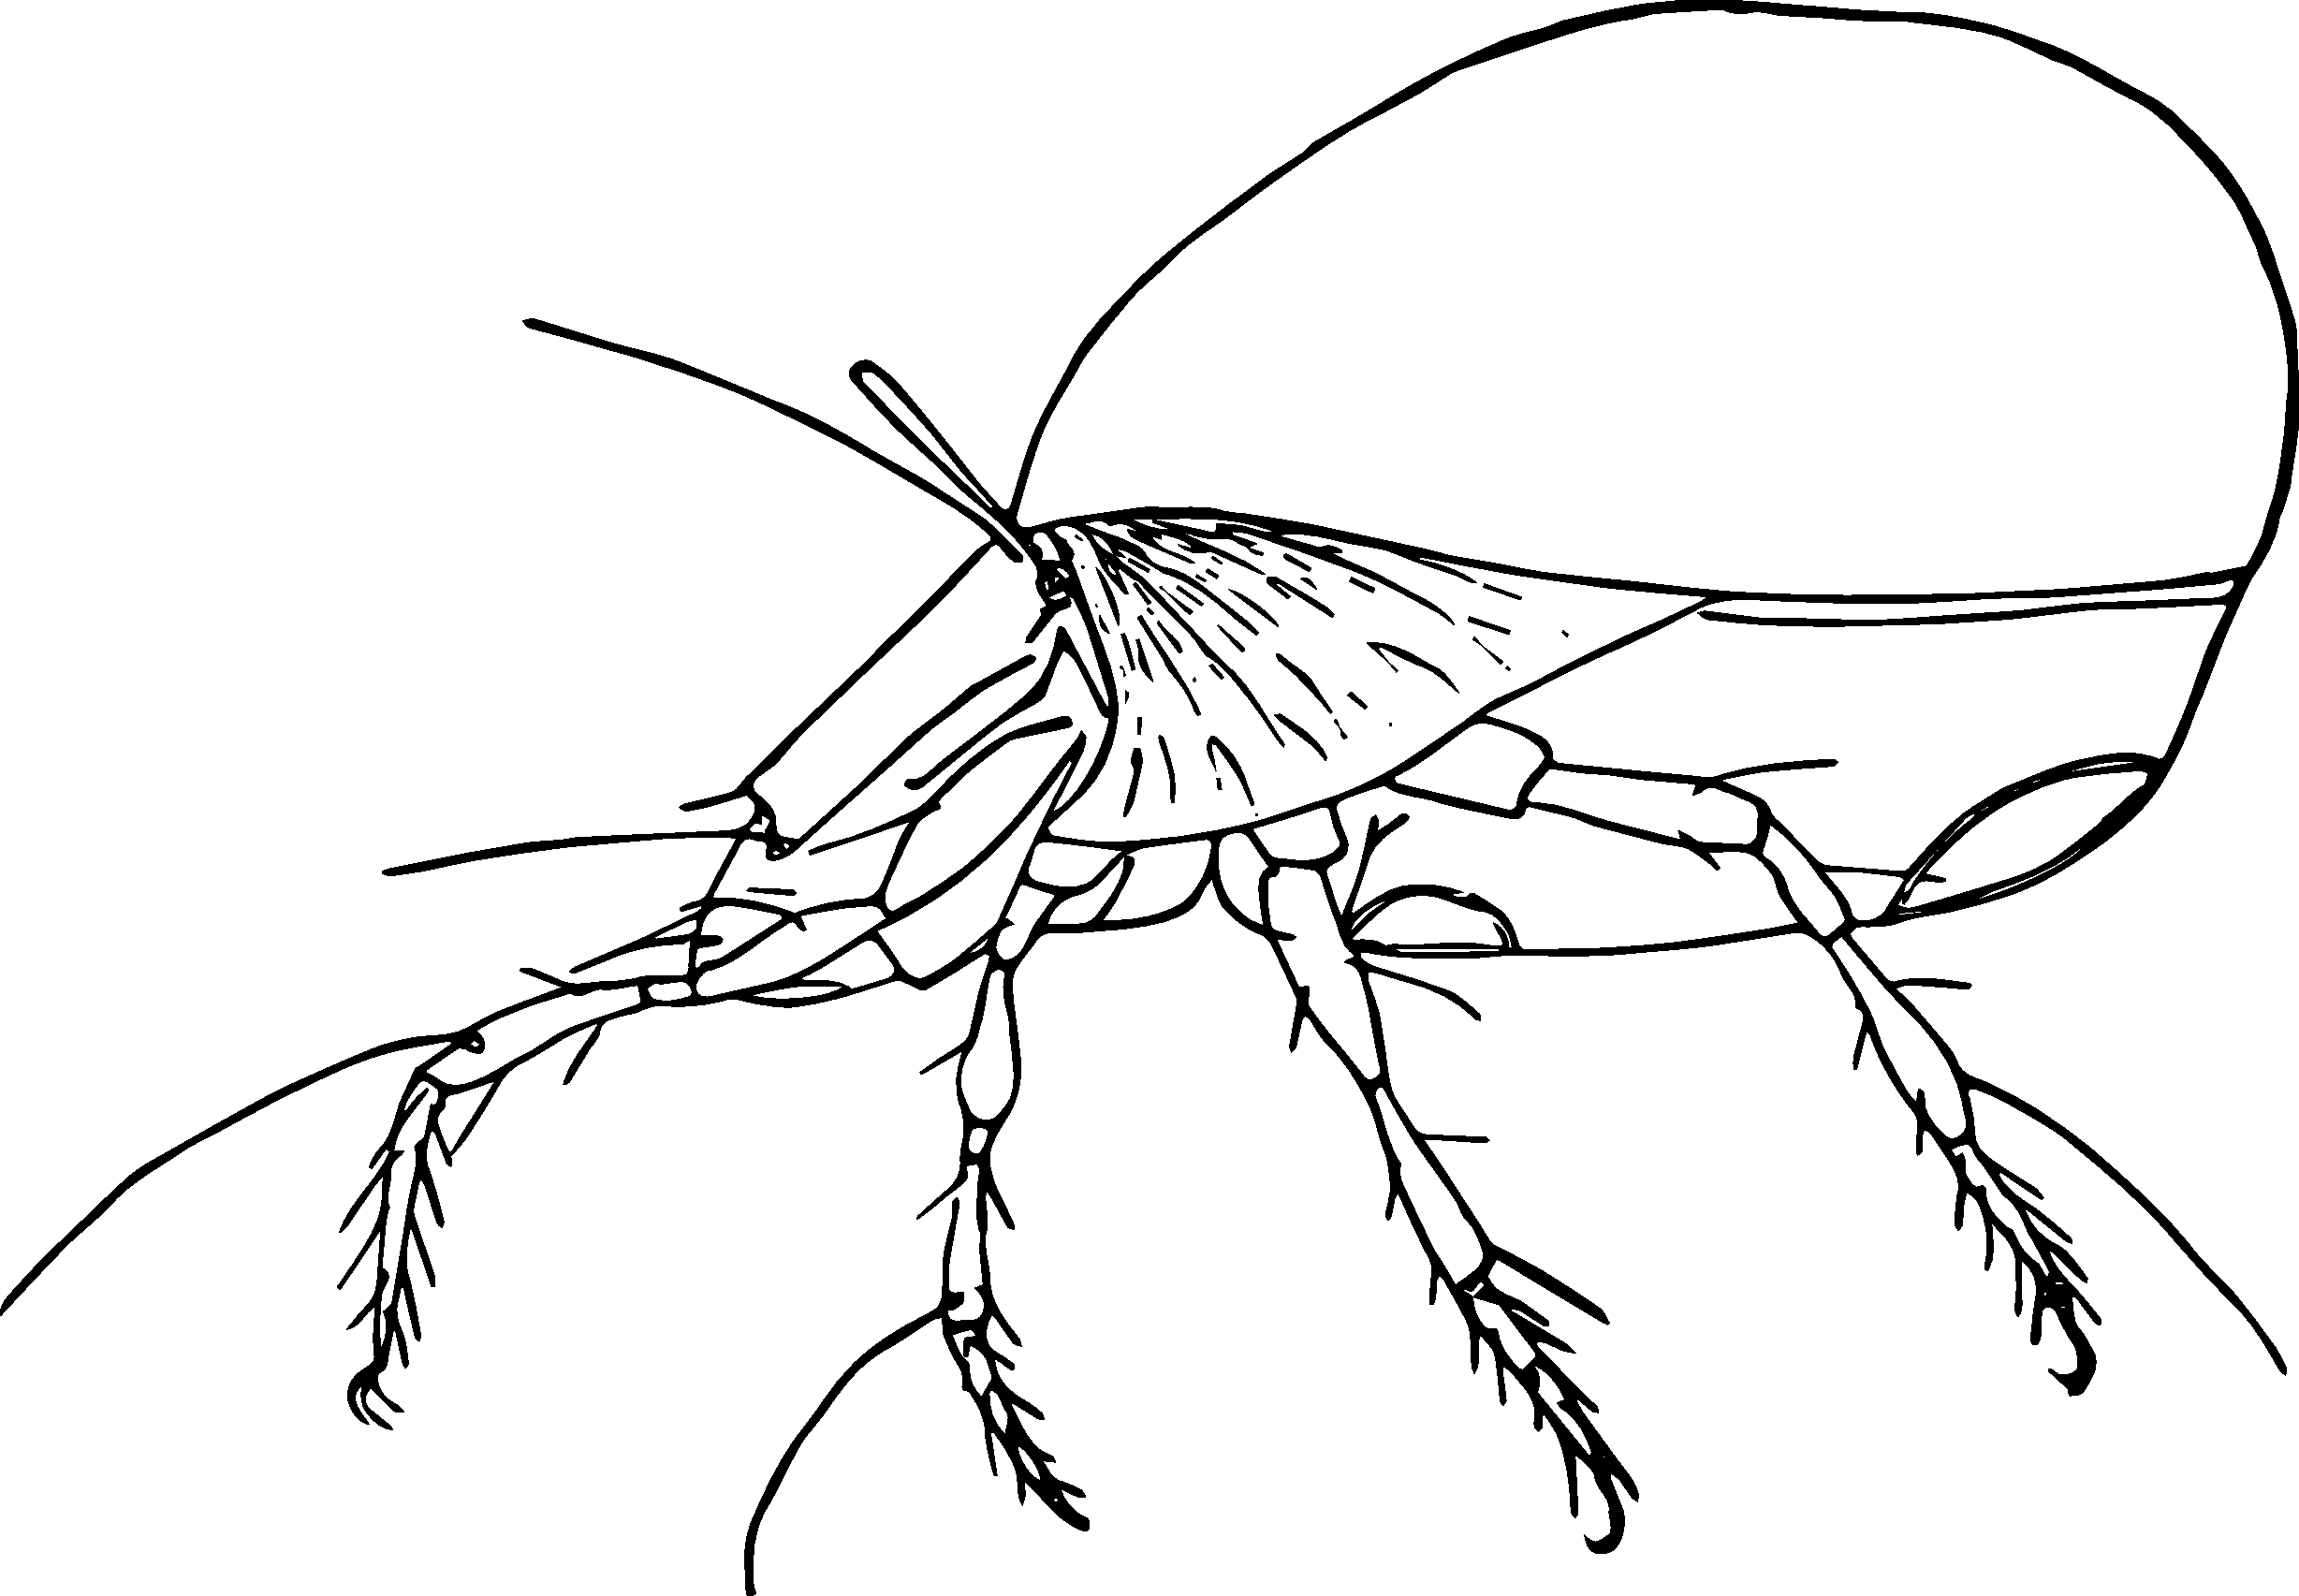
\includegraphics[width=\textwidth]{nonhexapod/oribatid}}
        \caption{}
        \label{fig:mite1}
    \end{subfigure}
    \hfill
    \begin{subfigure}[ht!]{0.45\textwidth}
        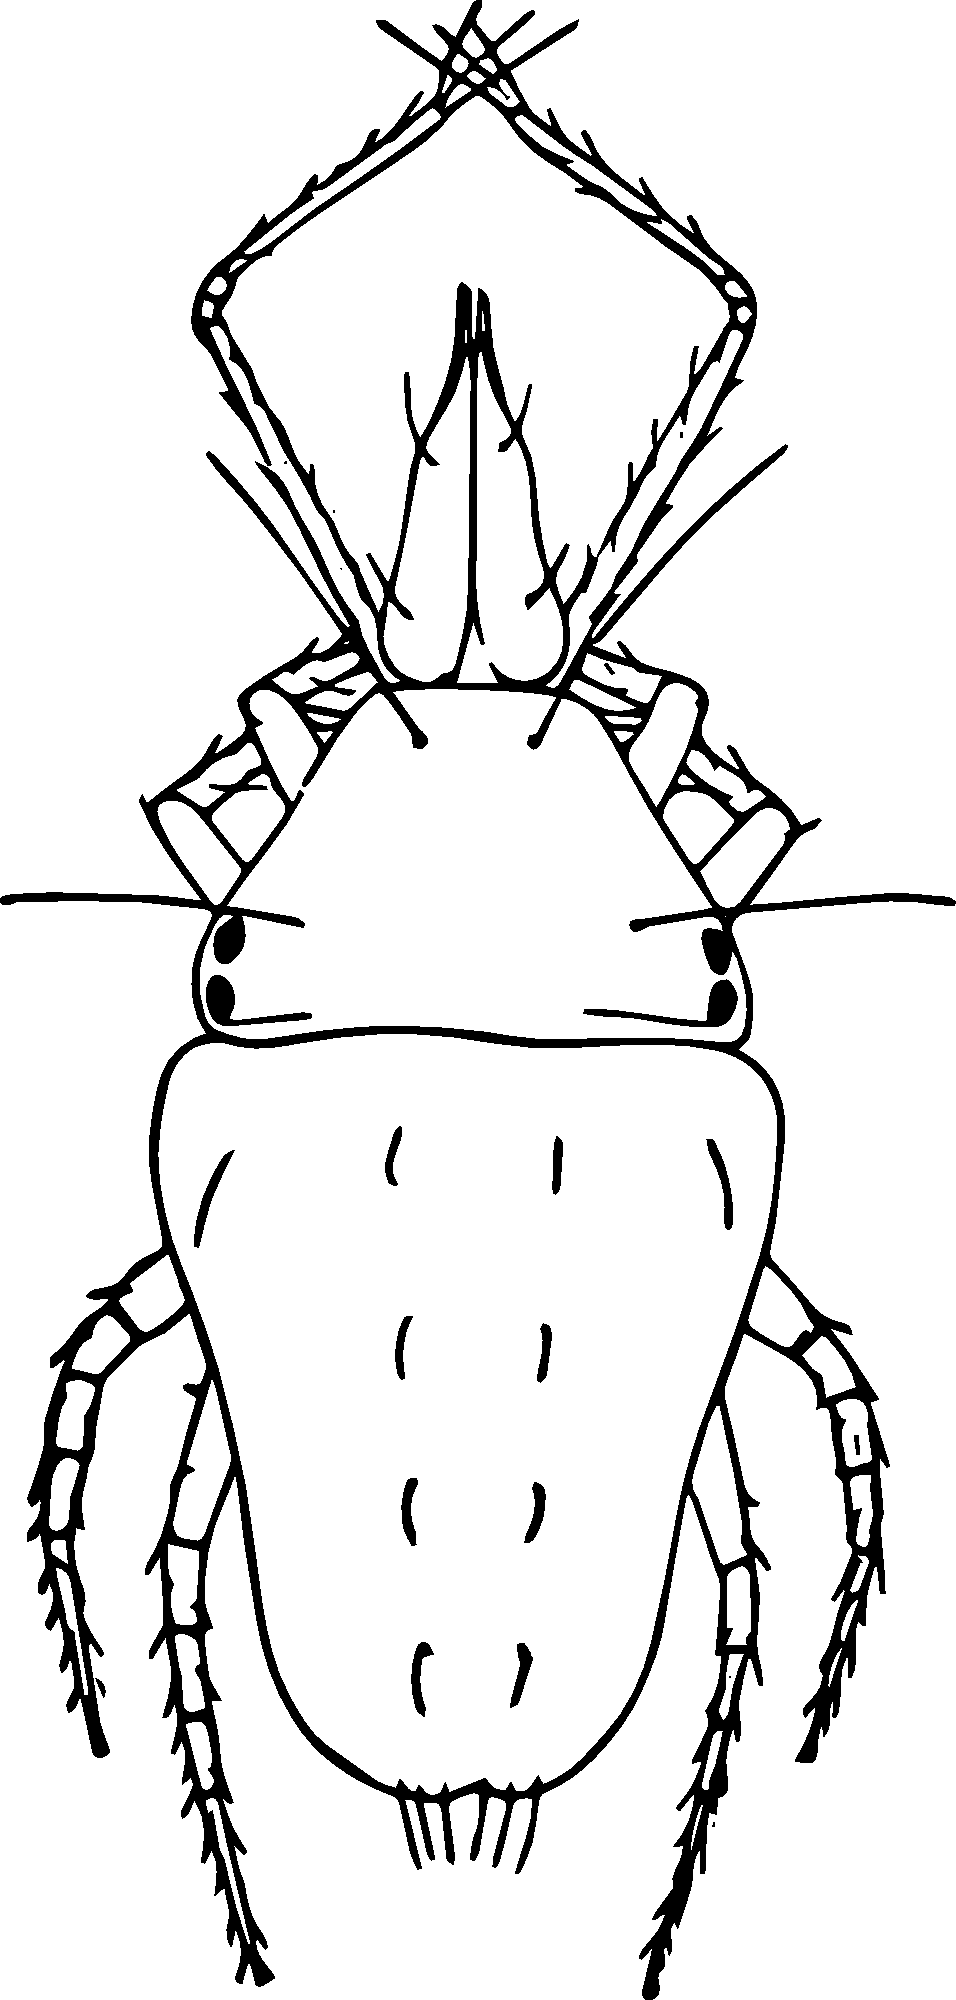
\includegraphics[angle=270,width=\textwidth]{nonhexapod/mite21}
        \caption{}
        \label{fig:mite2}
    \end{subfigure}
    \caption{Mites (Acari). \textbf{(a)} Lateral habitus of oribatid mite \citep[][Fig. 187]{bhlitem132773acari}; \textbf{(b)} dorsal habitus \citep[][Fig. 21]{bhlitem132773acari}} \label{fig:mites}
\end{figure}

\begin{figure}[ht!]
  \centering
    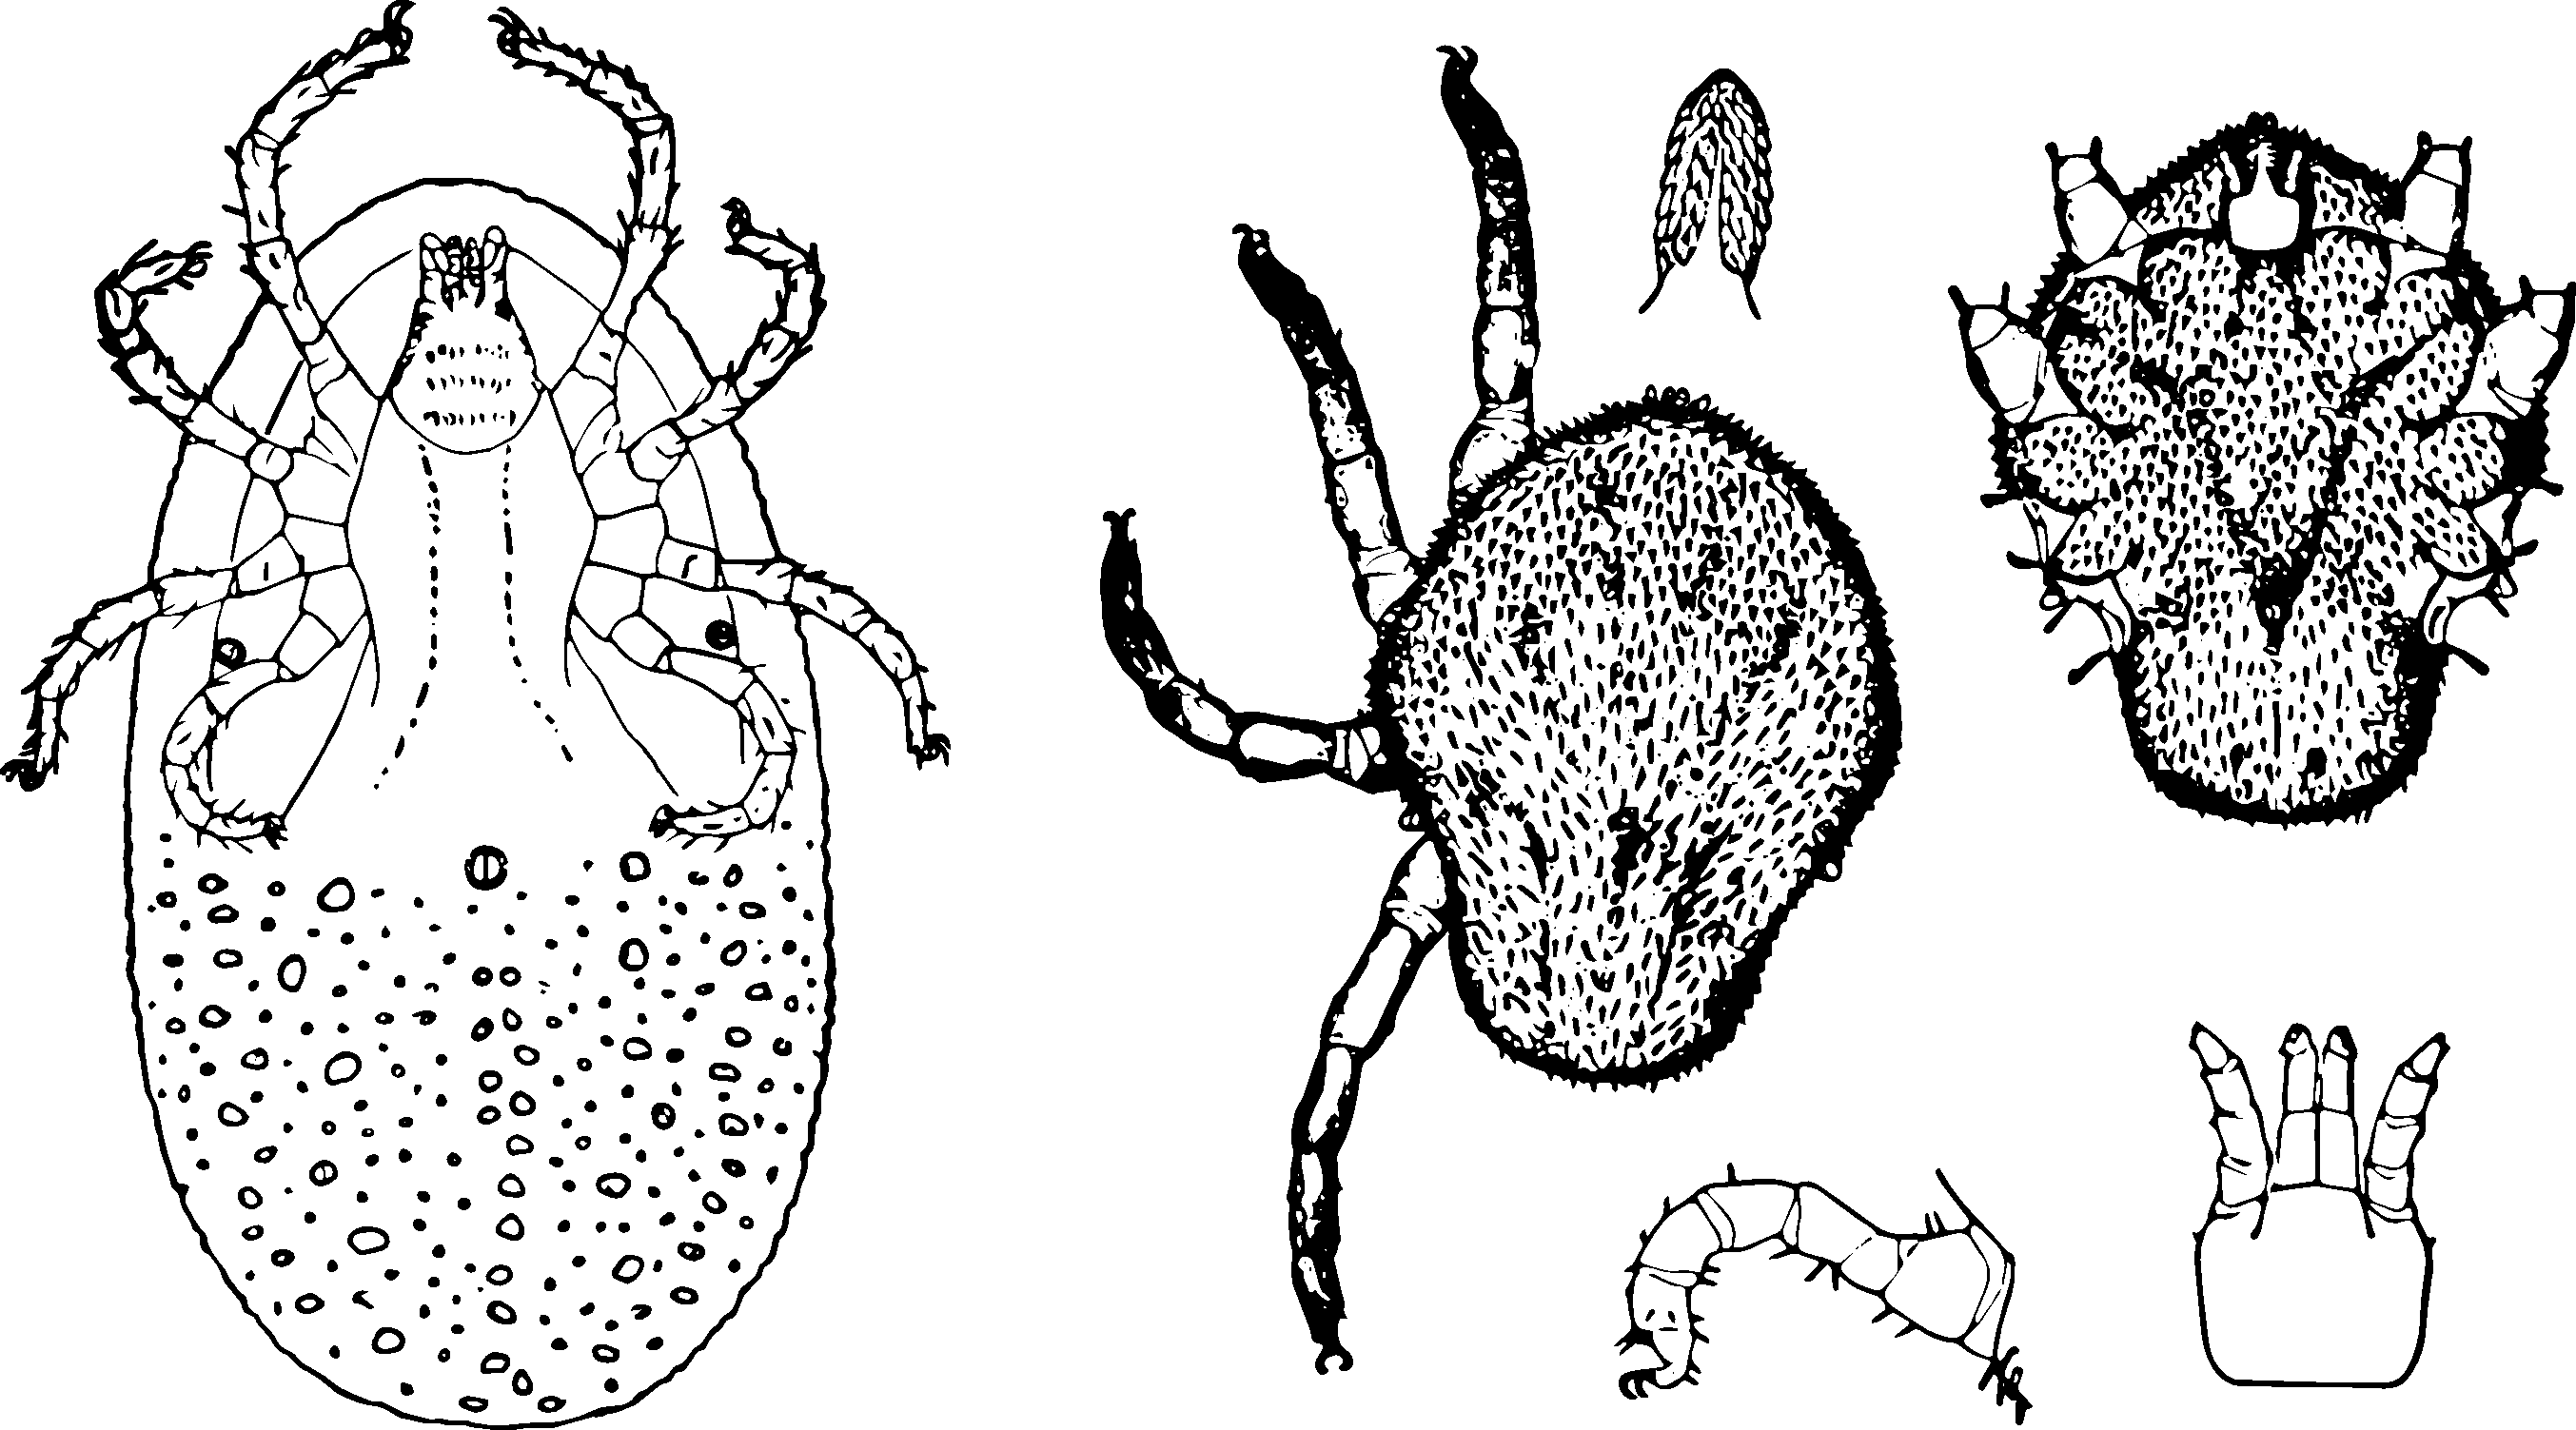
\includegraphics[width=0.65\textwidth]{nonhexapod/ixodid103104}
  \caption{Ticks \citep[][Figs. 103, 104]{bhlitem132773acari}}
  \label{fig:ixodid}
\end{figure}

\subsection{Opiliones (Phalangida, harvestmen, daddy-longlegs)}\index{Opiliones}
\noindent{}\textit{Diagnostic characters:} Chelicerae chelate; opisthosoma segmented, broadly joined to prosoma, without tail-like structure (telson) (figure \ref{fig:opiliones1}); body ovoid; body  \textless7 mm long usually, with leg span up to 160 mm; pedipalp morphology variable: usually thinner than legs, sometimes raptorial.\vspace{3mm}

\noindent{}\textit{Natural history:} Most species are predators and/or scavengers, feeding with a compound structure (stomotheca), formed, in part, by the proximal pedipalp and anteriormost leg segments. These arachnids lack venom and silk glands but do produce noxious defensive odors through scent gland openings (ozopores). There are more than 6,500 species.\vspace{3mm}

\begin{figure}[ht!]
  \centering
    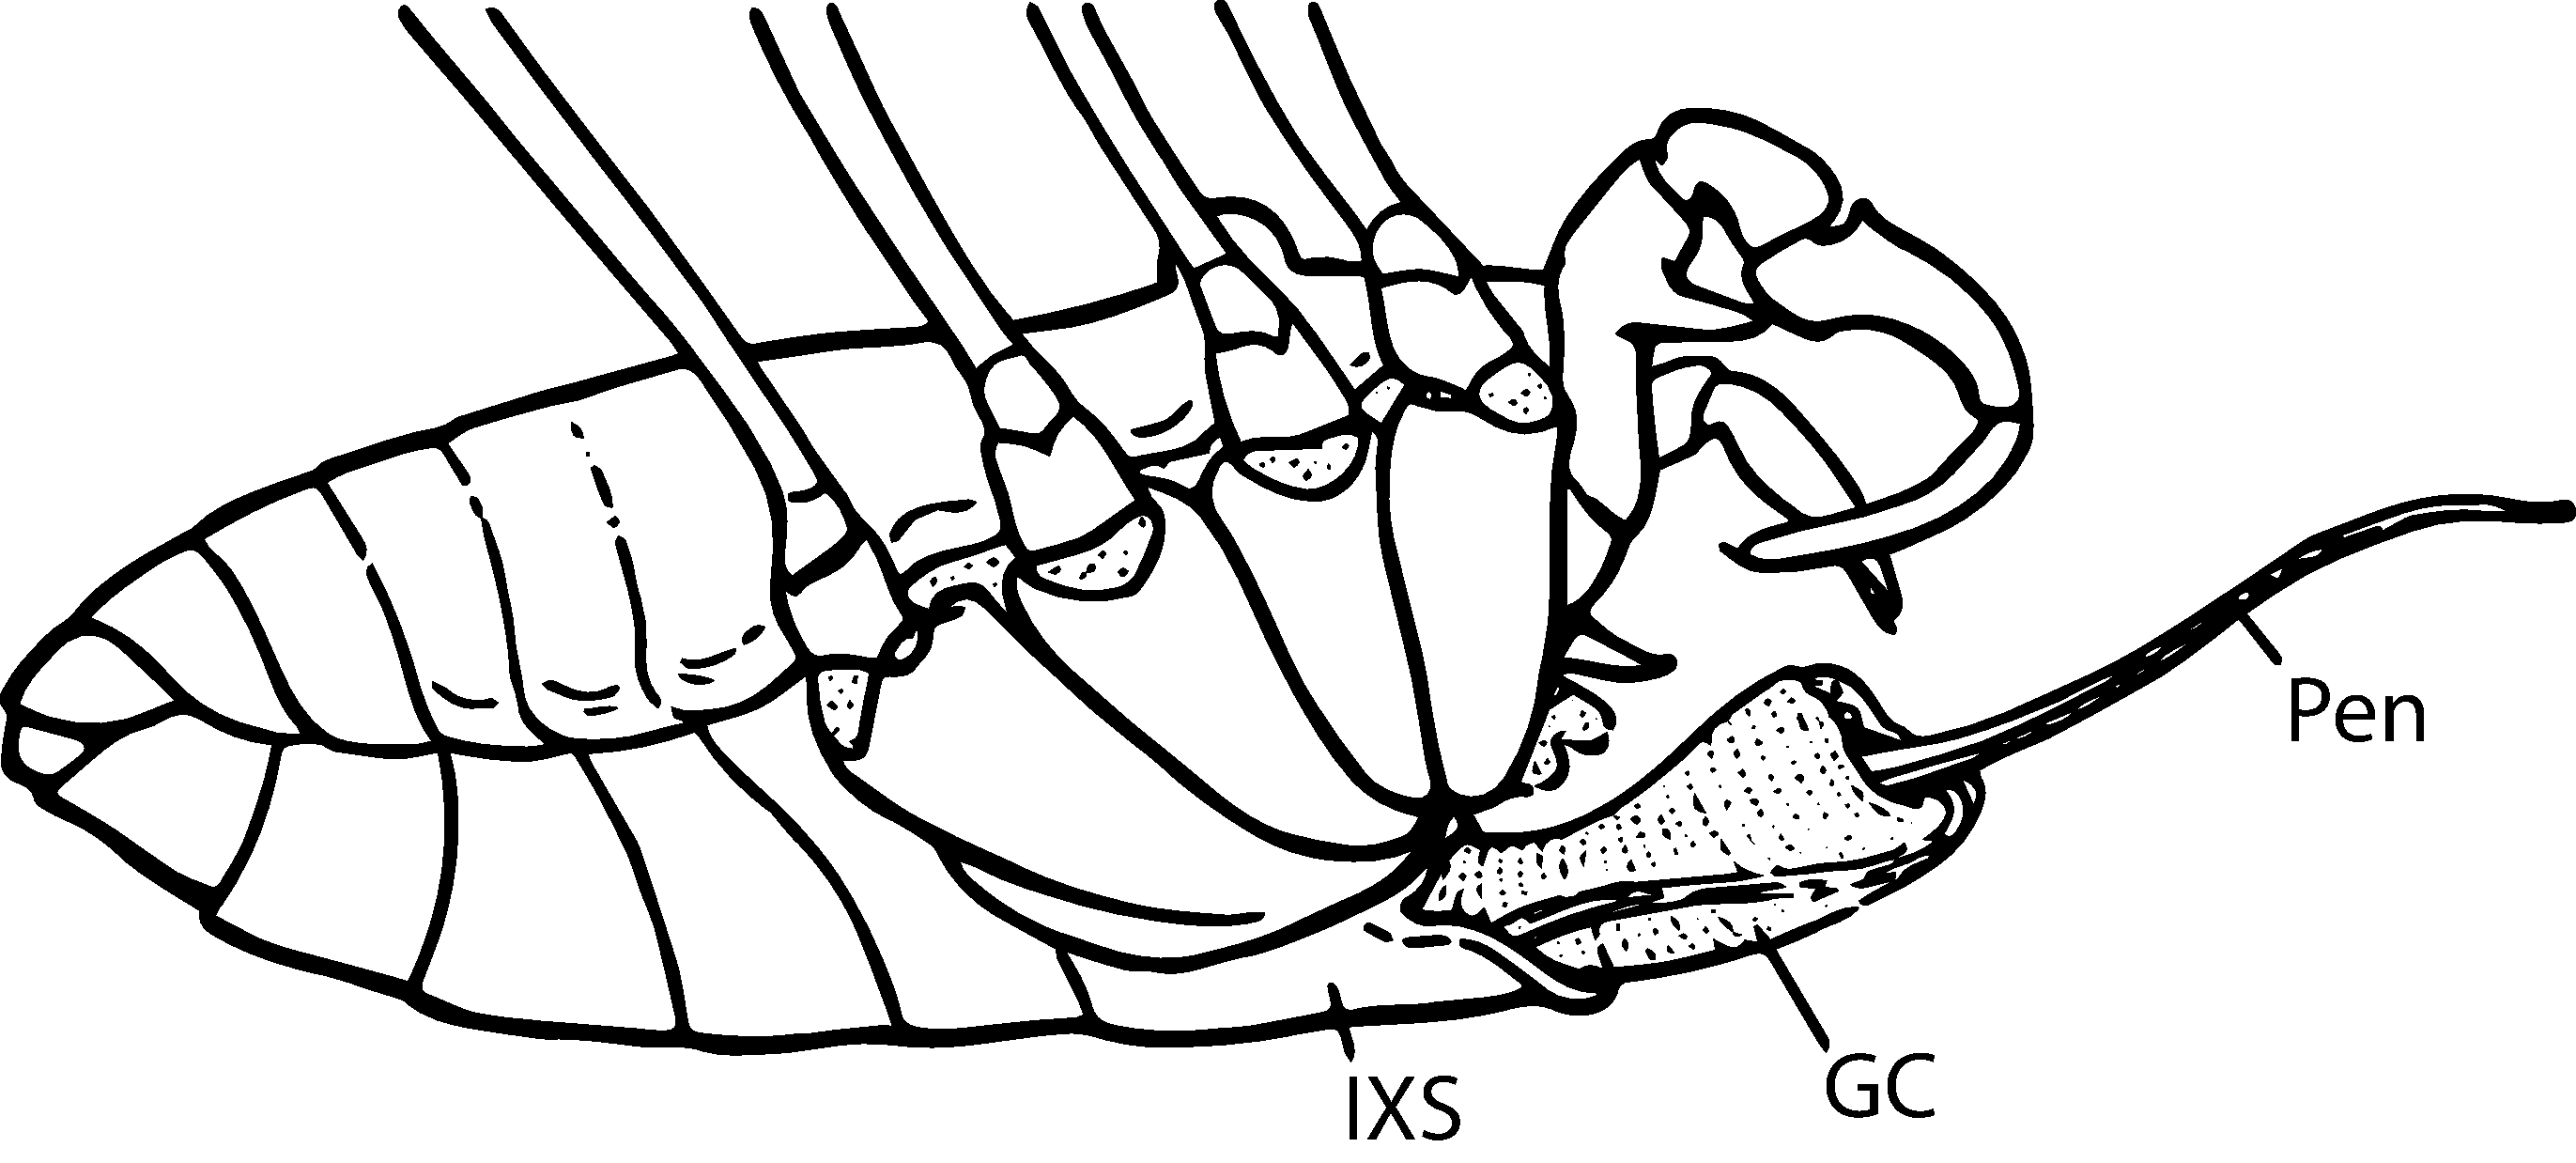
\includegraphics[width=0.6\textwidth]{nonhexapod/opilion12C}
  \caption{Opiliones lateral habitus. Pen = penis; GC = genital chamber; IXS = 9th segment sternum  \citep{snodgrass1937morphology}}
  \label{fig:opiliones1}
\end{figure}

\subsection{Scorpiones (scorpions)}\index{Scorpiones}
\noindent{}\textit{Diagnostic characters:} Chelicerae chelate; pedipalps long, chelate, and usually at least as thick as legs (figure \ref{fig:scorpion}); anteriormost pair of legs used for walking (\textit{i.e.}, not antenniform); opisthosoma segmented, broadly joined to prosoma; tail-like posteriorly (tail = \latinword{telson}); telson with venom gland and \latinword{stinger} present; 2nd segment of opisthosoma with comb-like sensory organs (pectines) ventrally.\vspace{3mm}

\noindent{}\textit{Natural history:} There are more than 1,700 species found worldwide, all of which are predators.\vspace{3mm}

\begin{figure}[ht!]
  \centering
    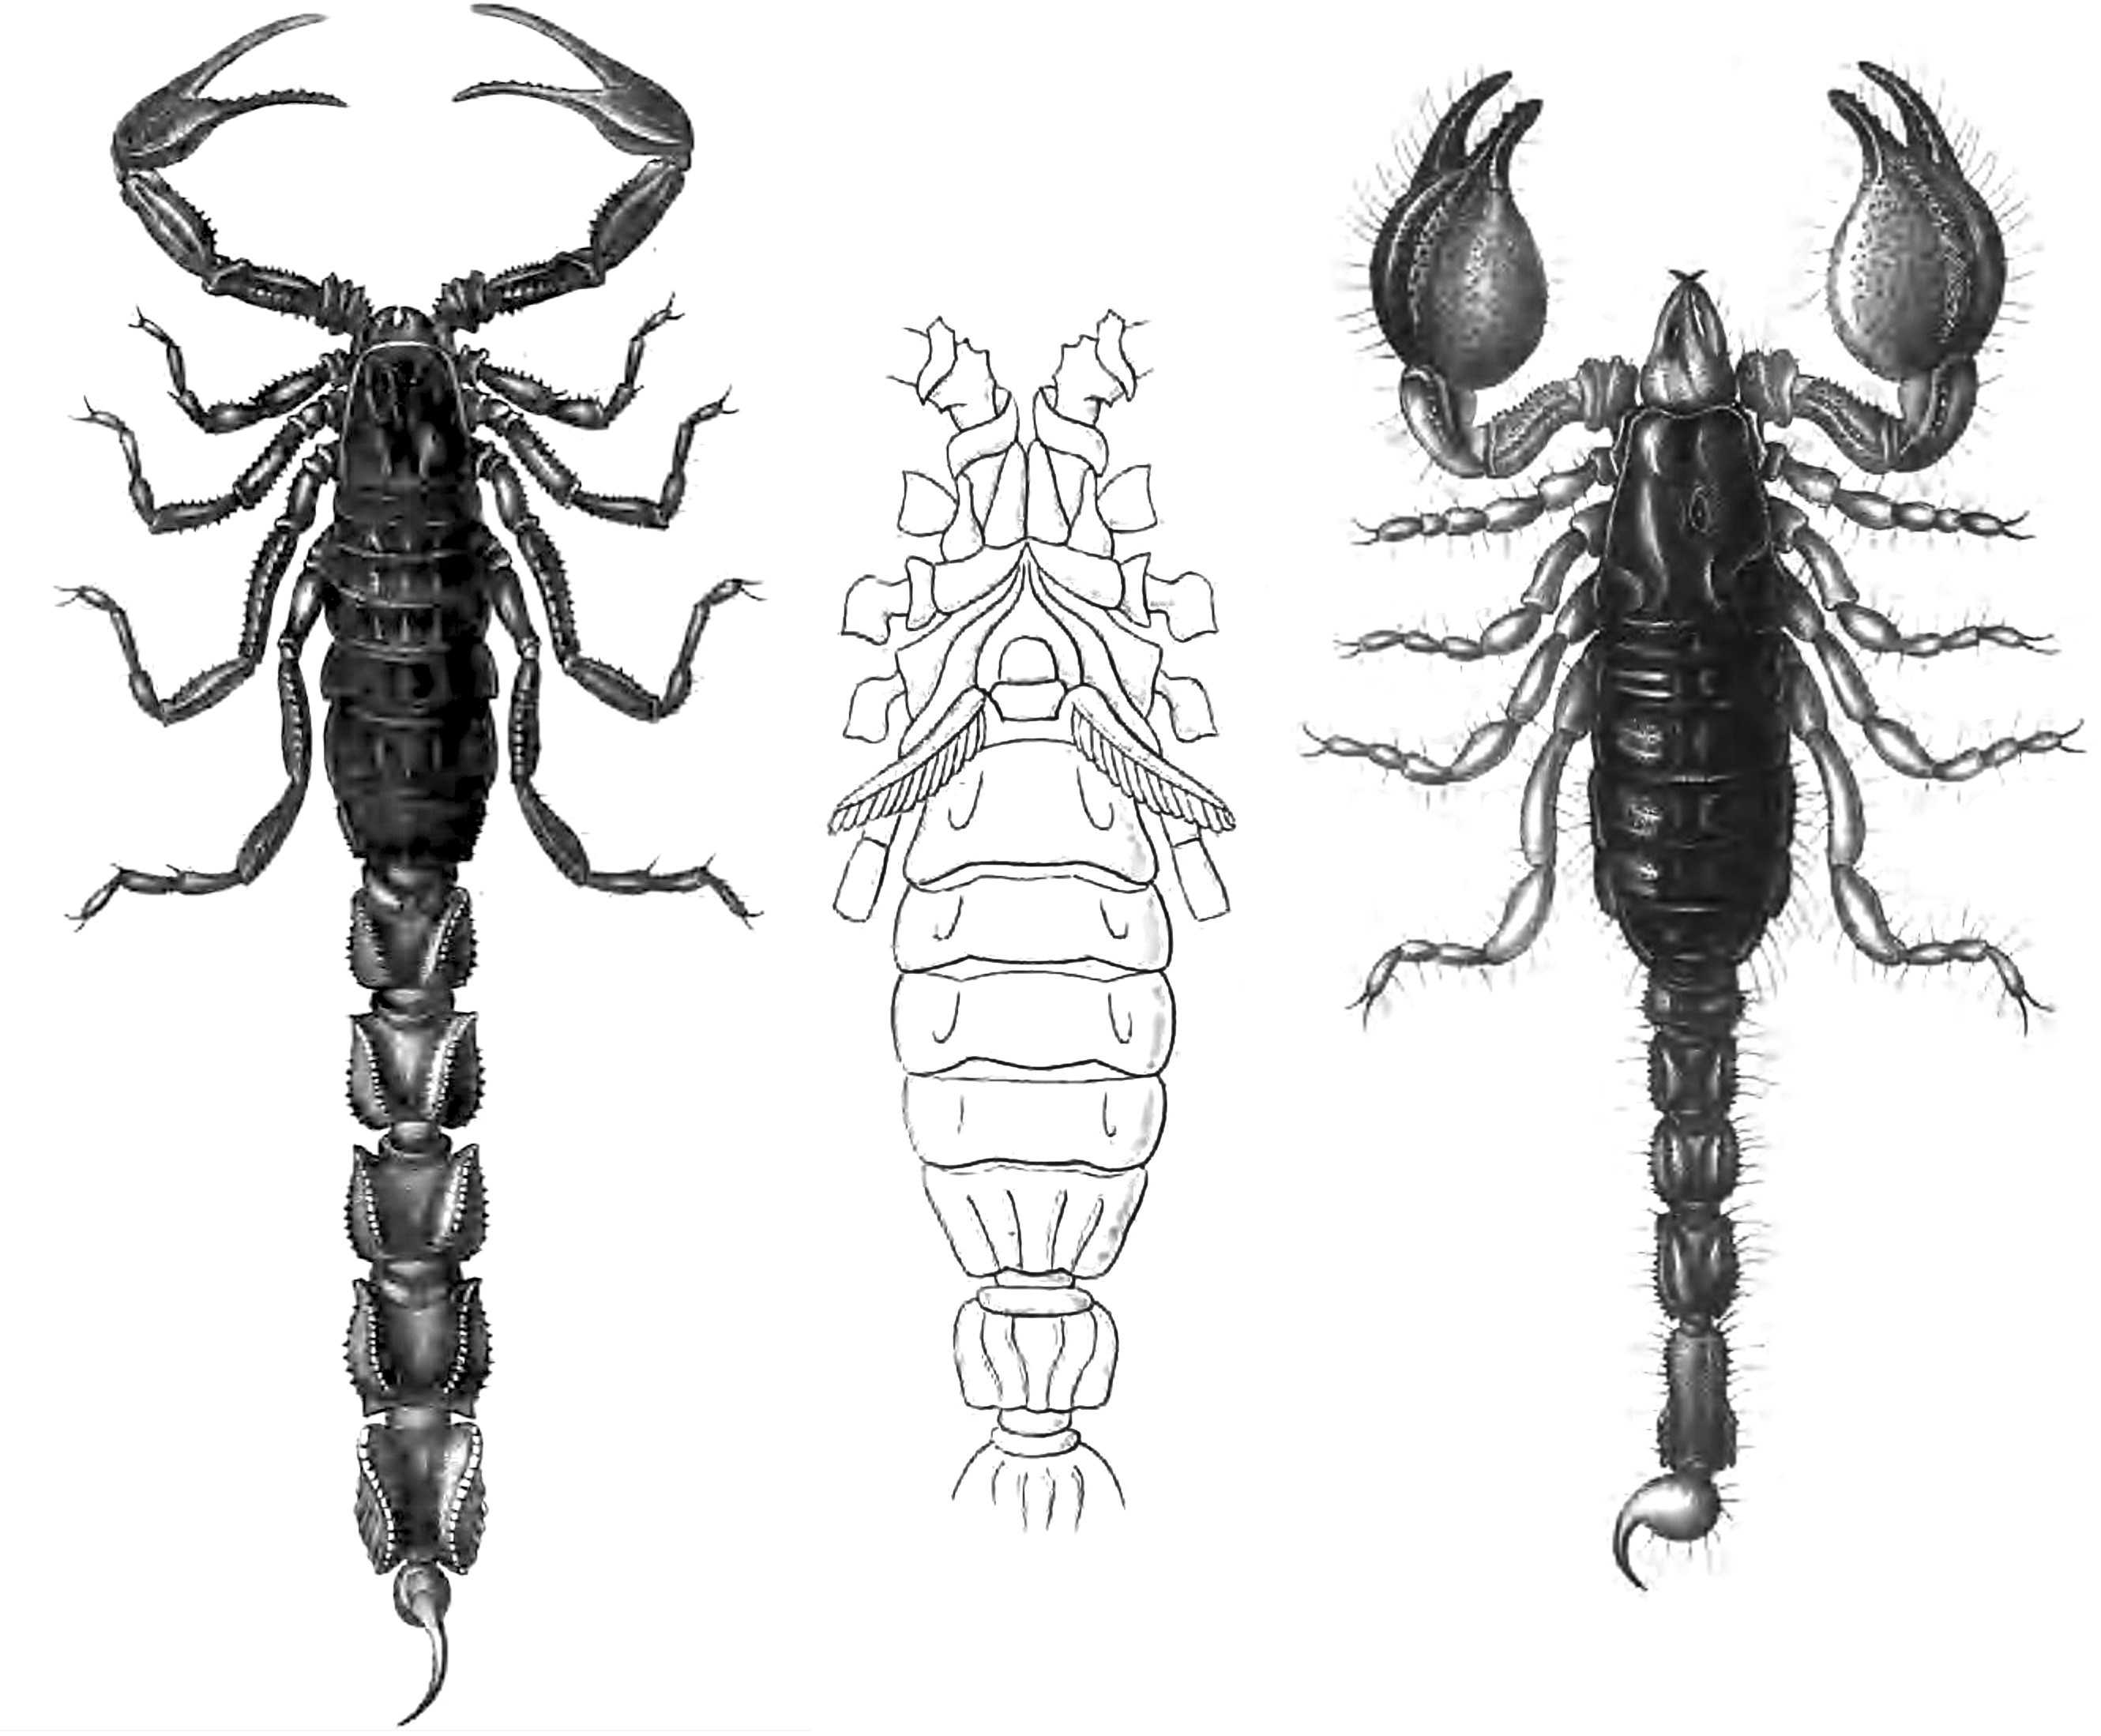
\includegraphics[width=0.7\textwidth]{nonhexapod/scorpions}
  \caption{Scorpiones \cite[][Plate 18, Figs. 1, 1b, 2]{bhlitem239255}}
  \label{fig:scorpion}
\end{figure}

\begin{theo}
{}Some scorpion species have massive pedipalps and relatively small telsons, while others exhibit the opposite set of phenotypes (\textit{i.e.}, massive telsons but small pedipalps; see figure \ref{fig:scorpion}). From a natural history perspective, what do you think is happening with these structures? Also, how do you think scorpions find prey?
\end{theo} %see https://doi.org/10.3389/fevo.2019.00196 / https://doi.org/10.1371/journal.pone.0078955

\subsection{Pseudoscorpiones (Pseudoscorpionida, Chelonethida, pseudoscorpions)}\index{Pseudoscorpiones}
\noindent{}\textit{Diagnostic characters:} Chelicerae chelate; pedipalps long, chelate, and thicker than legs (figure \ref{fig:pseudo}); anteriormost pair of legs used for walking (\textit{i.e.}, not antenniform); opisthosoma segmented, broadly joined to prosoma, without telson; patellar segment absent on legs.\vspace{3mm}

\noindent{}\textit{Natural history:} There are 3,300 species of pseudoscorpion, most of which are relatively small (\textless5 mm long). Sometimes they can be found clinging to insects, hitching a ride (phoresy) or possibly eating parasitic mites (phagophilia). Some species subdue prey with venom, from a gland in the pedipalp.\vspace{3mm}

\begin{figure}[ht!]
  \centering
    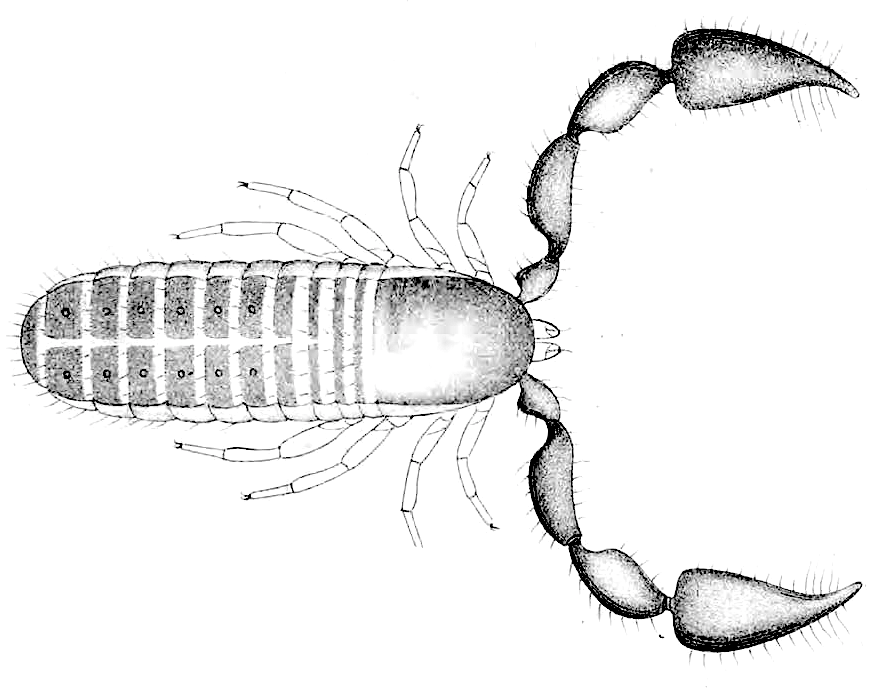
\includegraphics[width=0.4\textwidth]{nonhexapod/pseudoscorppl4fig6}
  \caption{Pseudoscorpiones \citep[][Plate IV, Fig. 6]{bhlitem260979pseudo}}
  \label{fig:pseudo}
\end{figure}

\section{Myriapoda}\index{Myriapoda}
\begin{itemize}
\item antennae present as single pair
\item appendages uniramous (\textit{i.e.}, no branches)
\item mouthparts mandibulate (\textit{i.e.}, not chelicerate)
\end{itemize}

\subsection{Diplopoda (millipedes)}\index{Diplopoda}
\noindent{}\textit{Diagnostic characters:} Most (apparent) segments with 2 pairs of legs (figure \ref{fig:diplop2}); antennae usually 7-segmented, short; 30+ pairs of legs present usually; body usually round, tube-like; some species small, bristly (figure \ref{fig:diplop1}).\vspace{3mm}

\noindent{}\textit{Natural history:} Millipedes typically forage on rotting materials (saprophagy) and are important recyclers of nutritive material. Most species are harmless, although some are renown for excreting toxic compounds when handled. There are \textgreater12,000 species described worldwide.\vspace{3mm}

\begin{figure}[ht!]
    \centering
    \begin{subfigure}[ht!]{0.27\textwidth}
        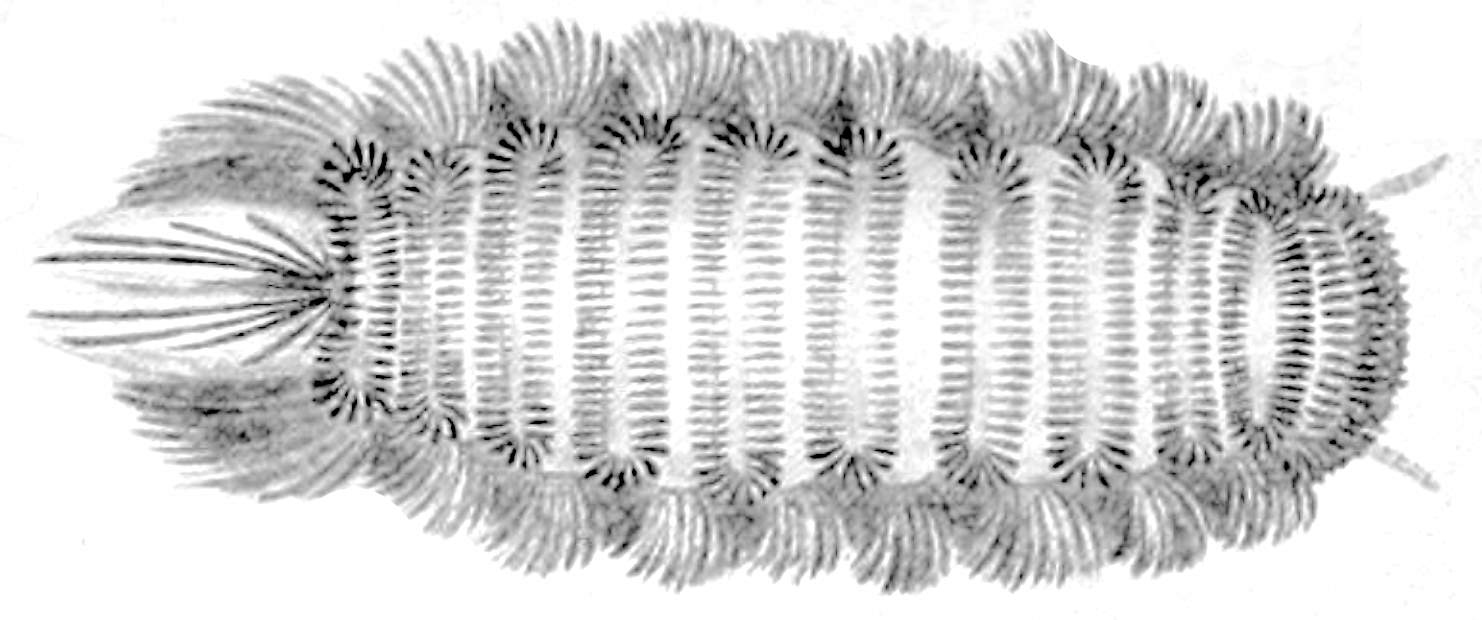
\includegraphics[width=\textwidth]{nonhexapod/diplopod82}
        \caption{}
        \label{fig:diplop1}
    \end{subfigure}
    \hfill
    \begin{subfigure}[ht!]{0.65\textwidth}
        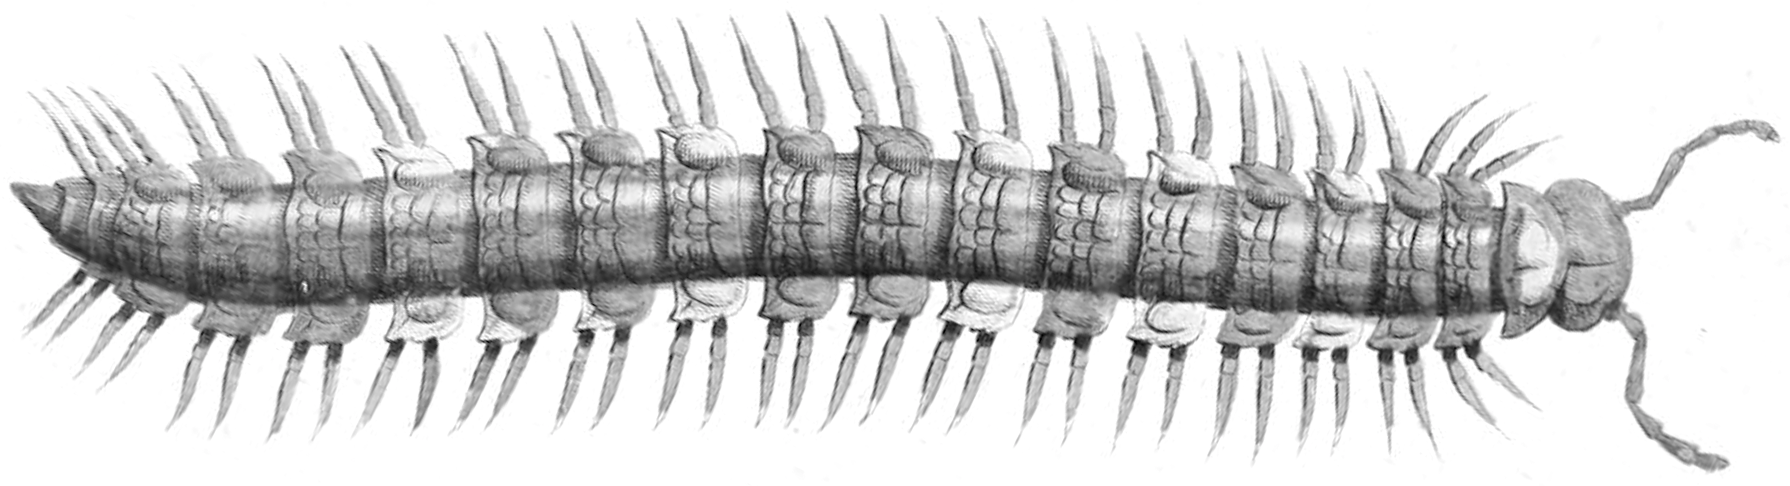
\includegraphics[width=\textwidth]{nonhexapod/millip}
        \caption{}
        \label{fig:diplop2}
    \end{subfigure}
    \caption{Millipedes (Diplopoda). \textbf{(a)} Bristle millipede (Polyxenida) \citep[][Fig. 82]{bhlitem40112britmus}; \textbf{(b)} Diplopoda \citep{bhlitem94979diplopo}} \label{fig:diplopoda}
\end{figure}

\subsection{Chilopoda (centipedes)}\index{Chilopoda}
\noindent{}\textit{Diagnostic characters:} Antennae usually with 14+ segments; apices of anteriormost pair of legs (\latinword{forcipules}) modified into fang-like structures (figure \ref{fig:chilo2}); most segments with 1 pair of legs; 15+ pairs of legs present usually (figure \ref{fig:chilo2}); body usually dorsoventrally flattened.\vspace{3mm}

\noindent{}\textit{Natural history:} These arthropods are predators of other organisms, including, in some cases, vertebrates. Prey are subdued with venom from the forcipules.\vspace{3mm}


\begin{figure}[ht!]
	\centering
        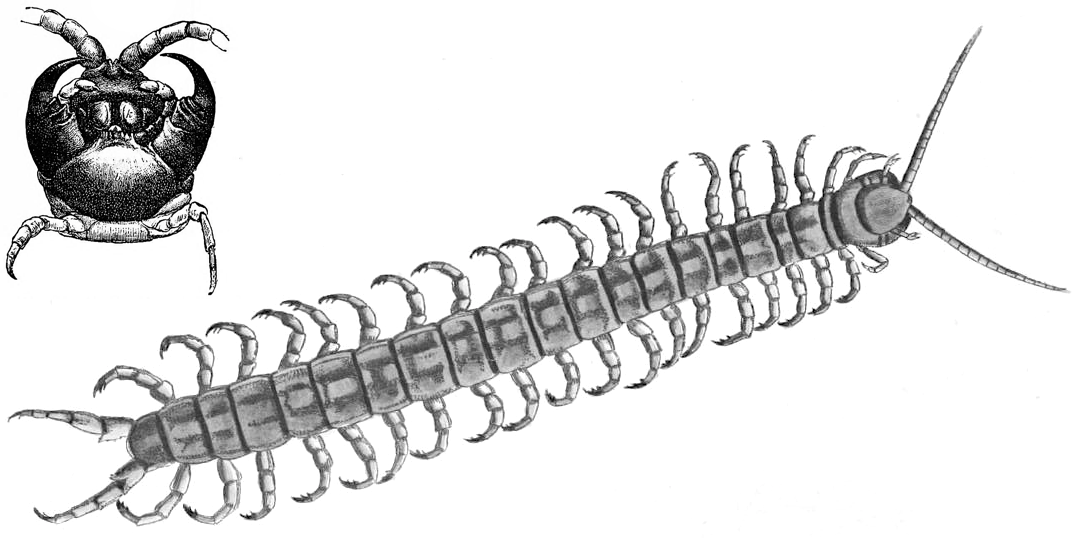
\includegraphics[width=0.8\textwidth]{nonhexapod/chilopod}
        \caption{Chilopoda. Modified from Fig. 138 in \cite{bhlitem91180chilopod} and, top left, Fig. 192 in \cite{bhlitem117775chilo2}}
        \label{fig:chilo2}
\end{figure}

\begin{theo}
{}Why do myriapods have so many legs? What advantage(s) does this condition provide these arthropods?
\end{theo}

\section{Non-hexapod Pancrustacea (formerly ``Crustacea'')}\index{Crustacea}\index{Pancrustacea}
\begin{itemize}
\item often with 2 tagmata: cephalothorax and abdomen
\item many biramous (2-branched) appendages, usually with 2nd pair of antennae (antennules)
\item mouthparts mandibulate
\end{itemize}

\subsection{Isopoda (pillbugs, sowbugs)}\index{Isopoda}
\noindent{}\textit{Diagnostic characters:} Body with no carapace, usually dorso-ventrally flattened (figure \ref{fig:isopod2}); 7 pairs of thoracic legs; 2nd pair of antennae reduced.\vspace{3mm}

\noindent{}\textit{Natural history:} One of the few non-hexapod pancrustaceans to radiate in the terrestrial environment. Of the approximately 10,000 known species, about half are terrestrial. The rest are marine (about 4,500 spp.) or inhabit freshwater. Most species survive as scavengers but many are parasitic on fish or other aquatic organisms.\vspace{3mm}

\subsection{Amphipoda (scuds)}\index{Amphipoda}
\noindent{}\textit{Diagnostic characters:} No carapace, usually laterally flattened (figure \ref{fig:amphip}); fore legs often raptorial; usually 6 or 7 pairs of thoracic legs.\vspace{3mm}

\noindent{}\textit{Natural history:} Of the 9,500 known species, approximately 20\% are found in freshwater. The vast majority are marine, but a handful are terrestrial (usually closely associated with aquatic habitats). They are mostly scavengers.\vspace{3mm}

\begin{figure}[ht!]
    \centering
    \begin{subfigure}[ht!]{0.4\textwidth}\reflectbox{
        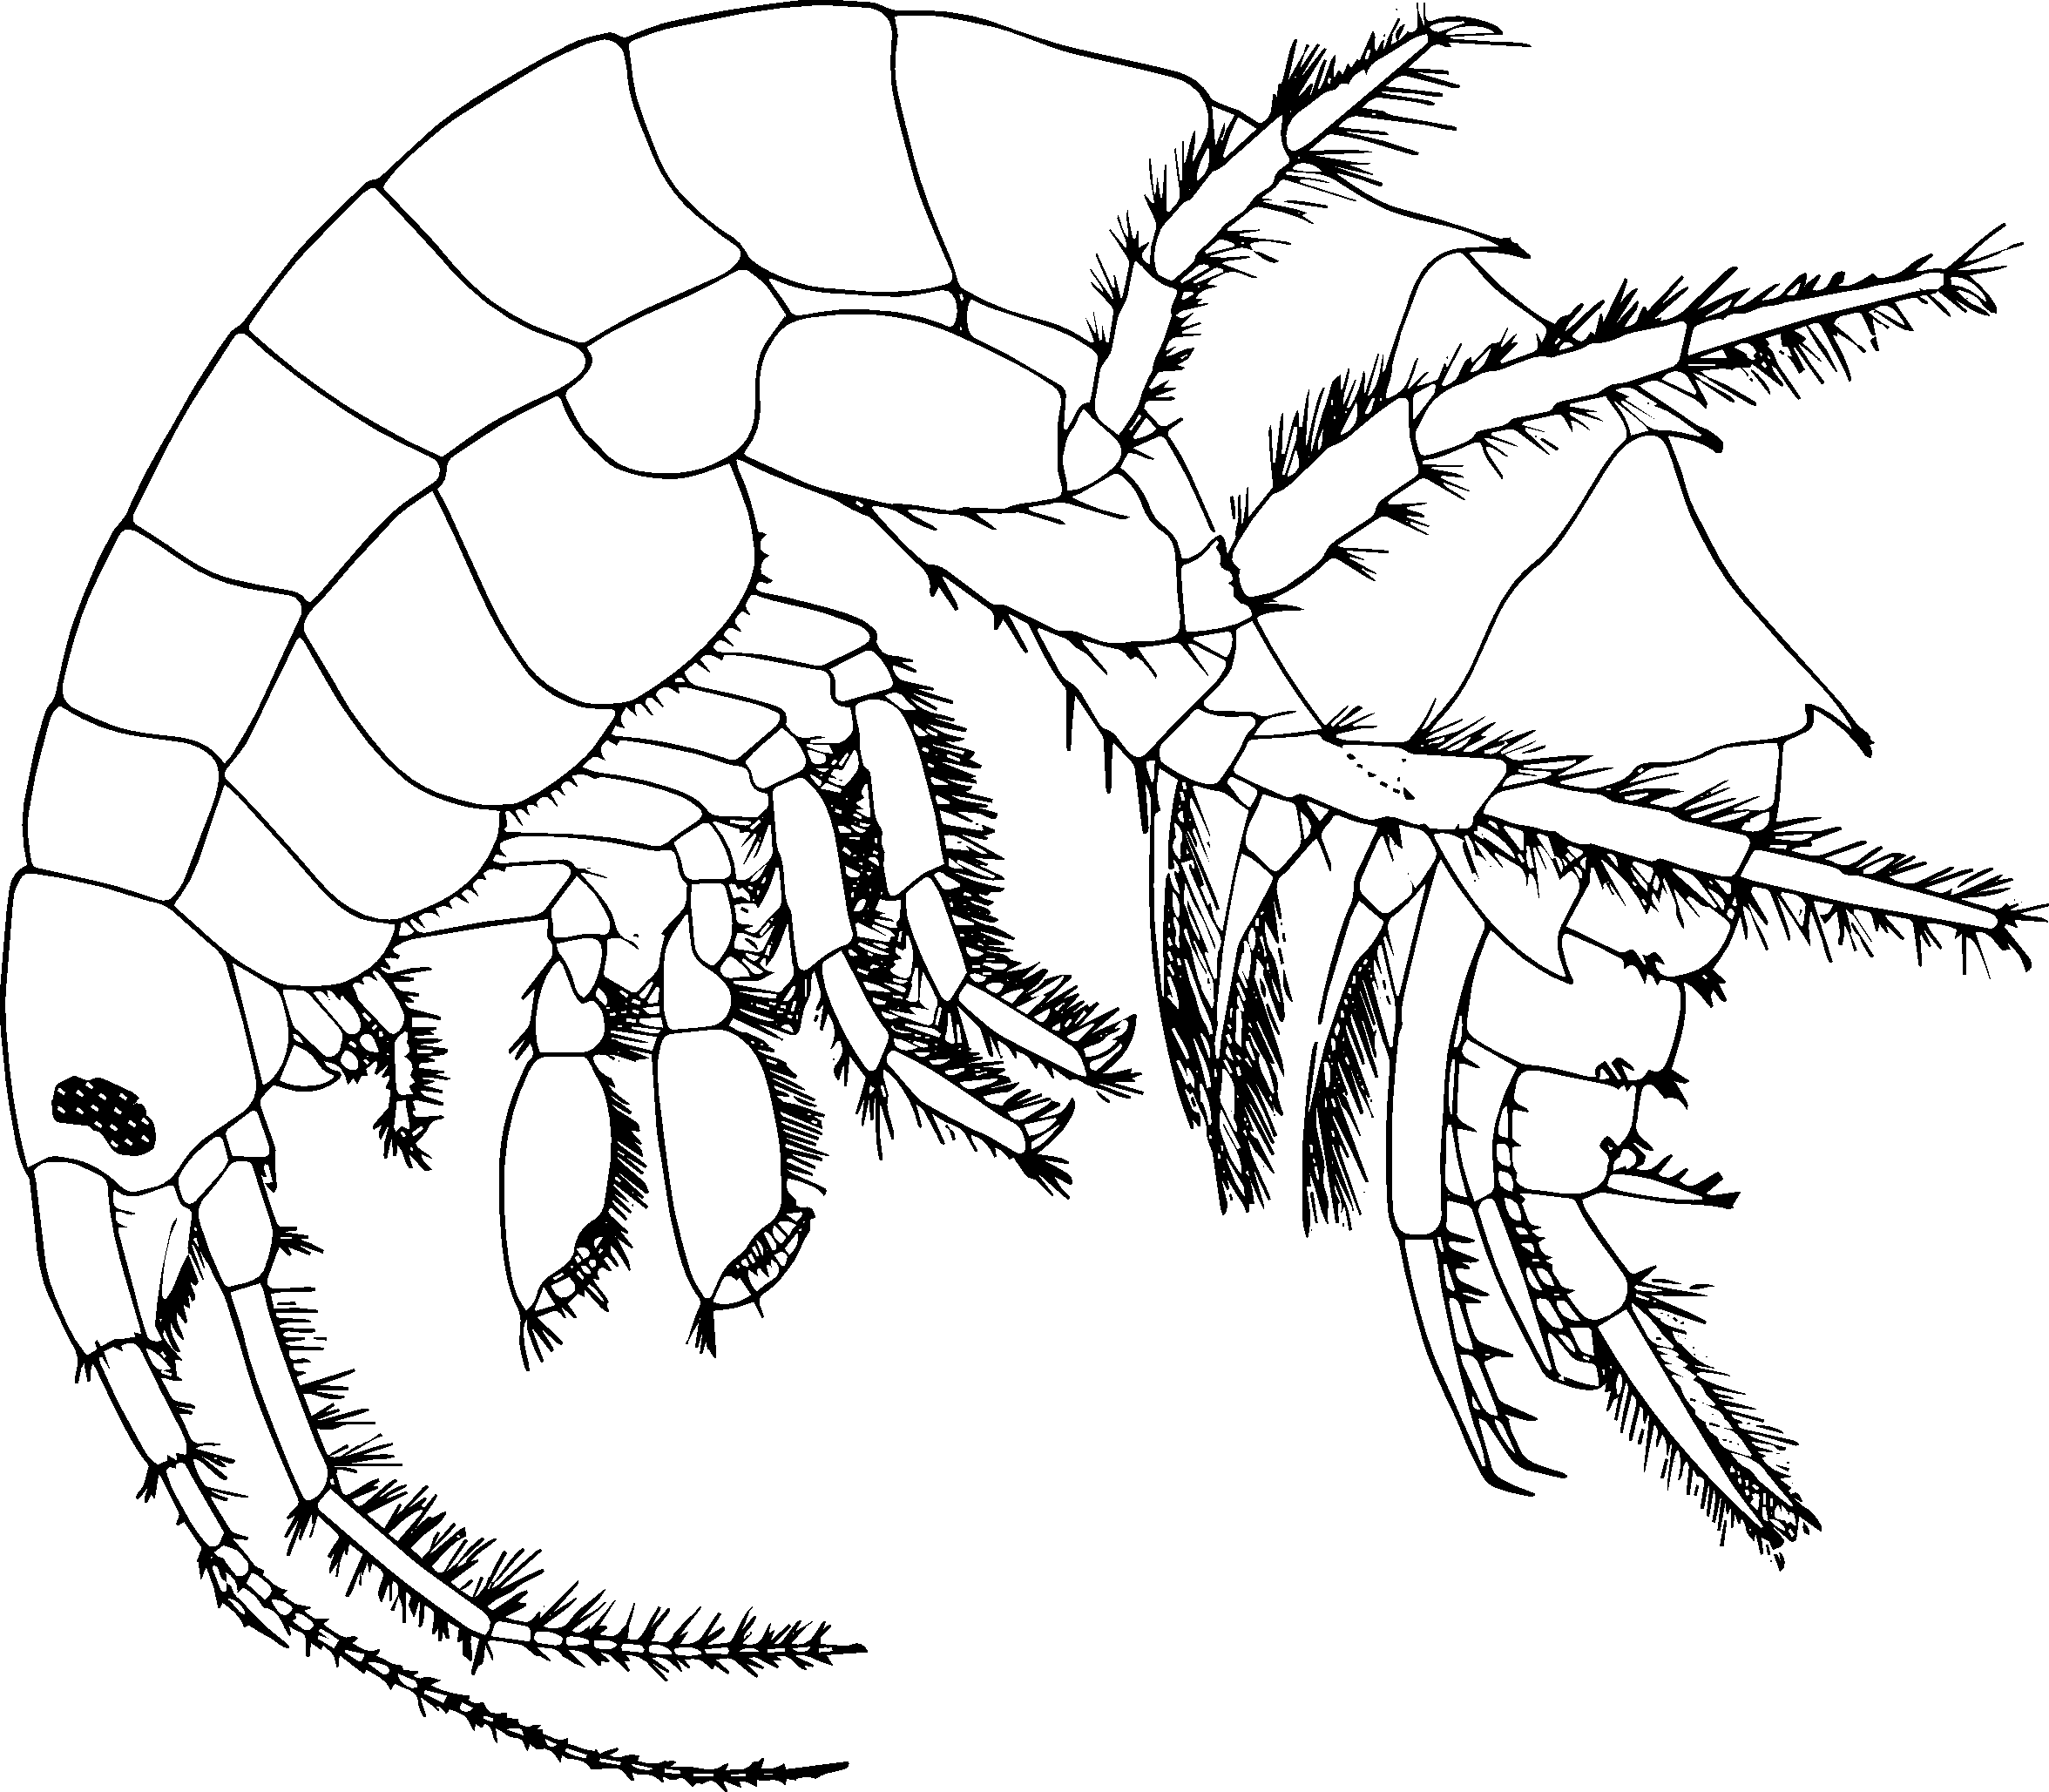
\includegraphics[width=\textwidth]{nonhexapod/amphipod30}}
        \caption{Amphipoda \citep[][Fig. 30]{bhlitem148531crust}}
        \label{fig:amphip}
    \end{subfigure}
    \hfill 
    \begin{subfigure}[ht!]{0.45\textwidth}
        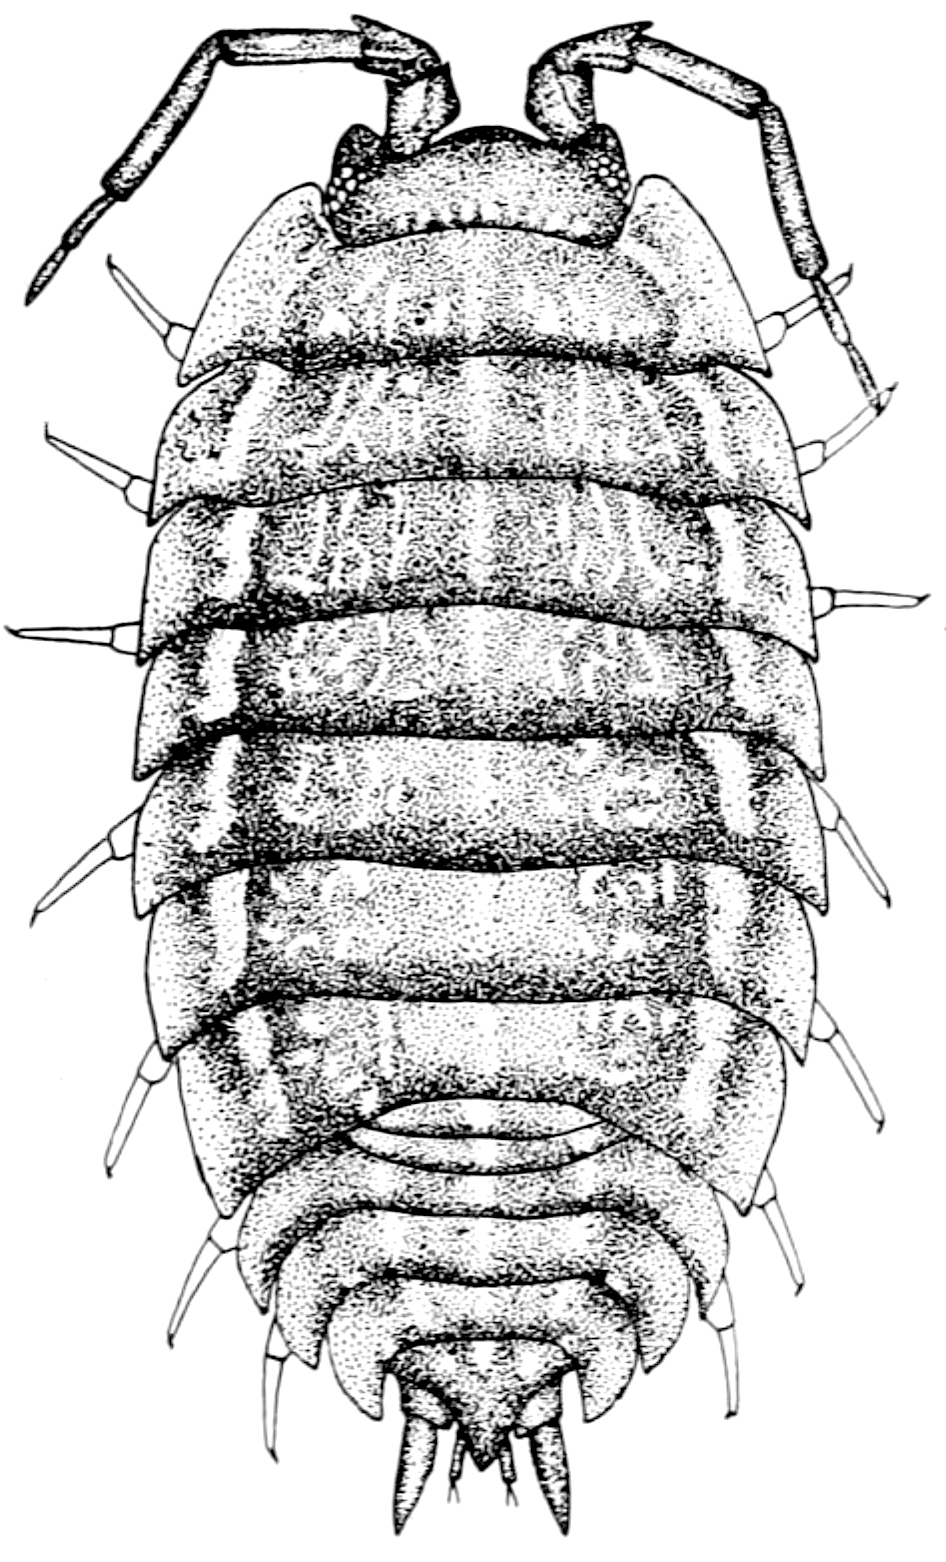
\includegraphics[angle=270,width=\textwidth]{nonhexapod/isopod55}
        \caption{Isopoda \citep[][Fig. 55]{bhlitem148531crust}}
        \label{fig:isopod2}
    \end{subfigure}
    \caption{``Crustacea''} 
\end{figure}

\subsection{Branchiopoda (fairy shrimp, clam shrimp)}\index{Branchiopoda}
\noindent{}\textit{Diagnostic characters:} Very diverse in habitus but usually with many appendages, each of which typically has a gill associated with it. Carapace usually prominent (figure \ref{fig:branchiopoda}), either as a shield-like sclerite or even as a hinged, bivalve-like sclerite.\vspace{3mm}

\noindent{}\textit{Natural history:} Aquatic but extraordinarily diverse in natural history. Typically feed on plankton and suspended organic matter, but some are predators and/or scavengers. Many species found in freshwater, and those that inhabit saline or brackish water are usually in continental water bodies (rather than in the ocean). Eggs of many species are capable of weathering hostile environments.\vspace{3mm}

\begin{figure}[ht!]
  \centering
    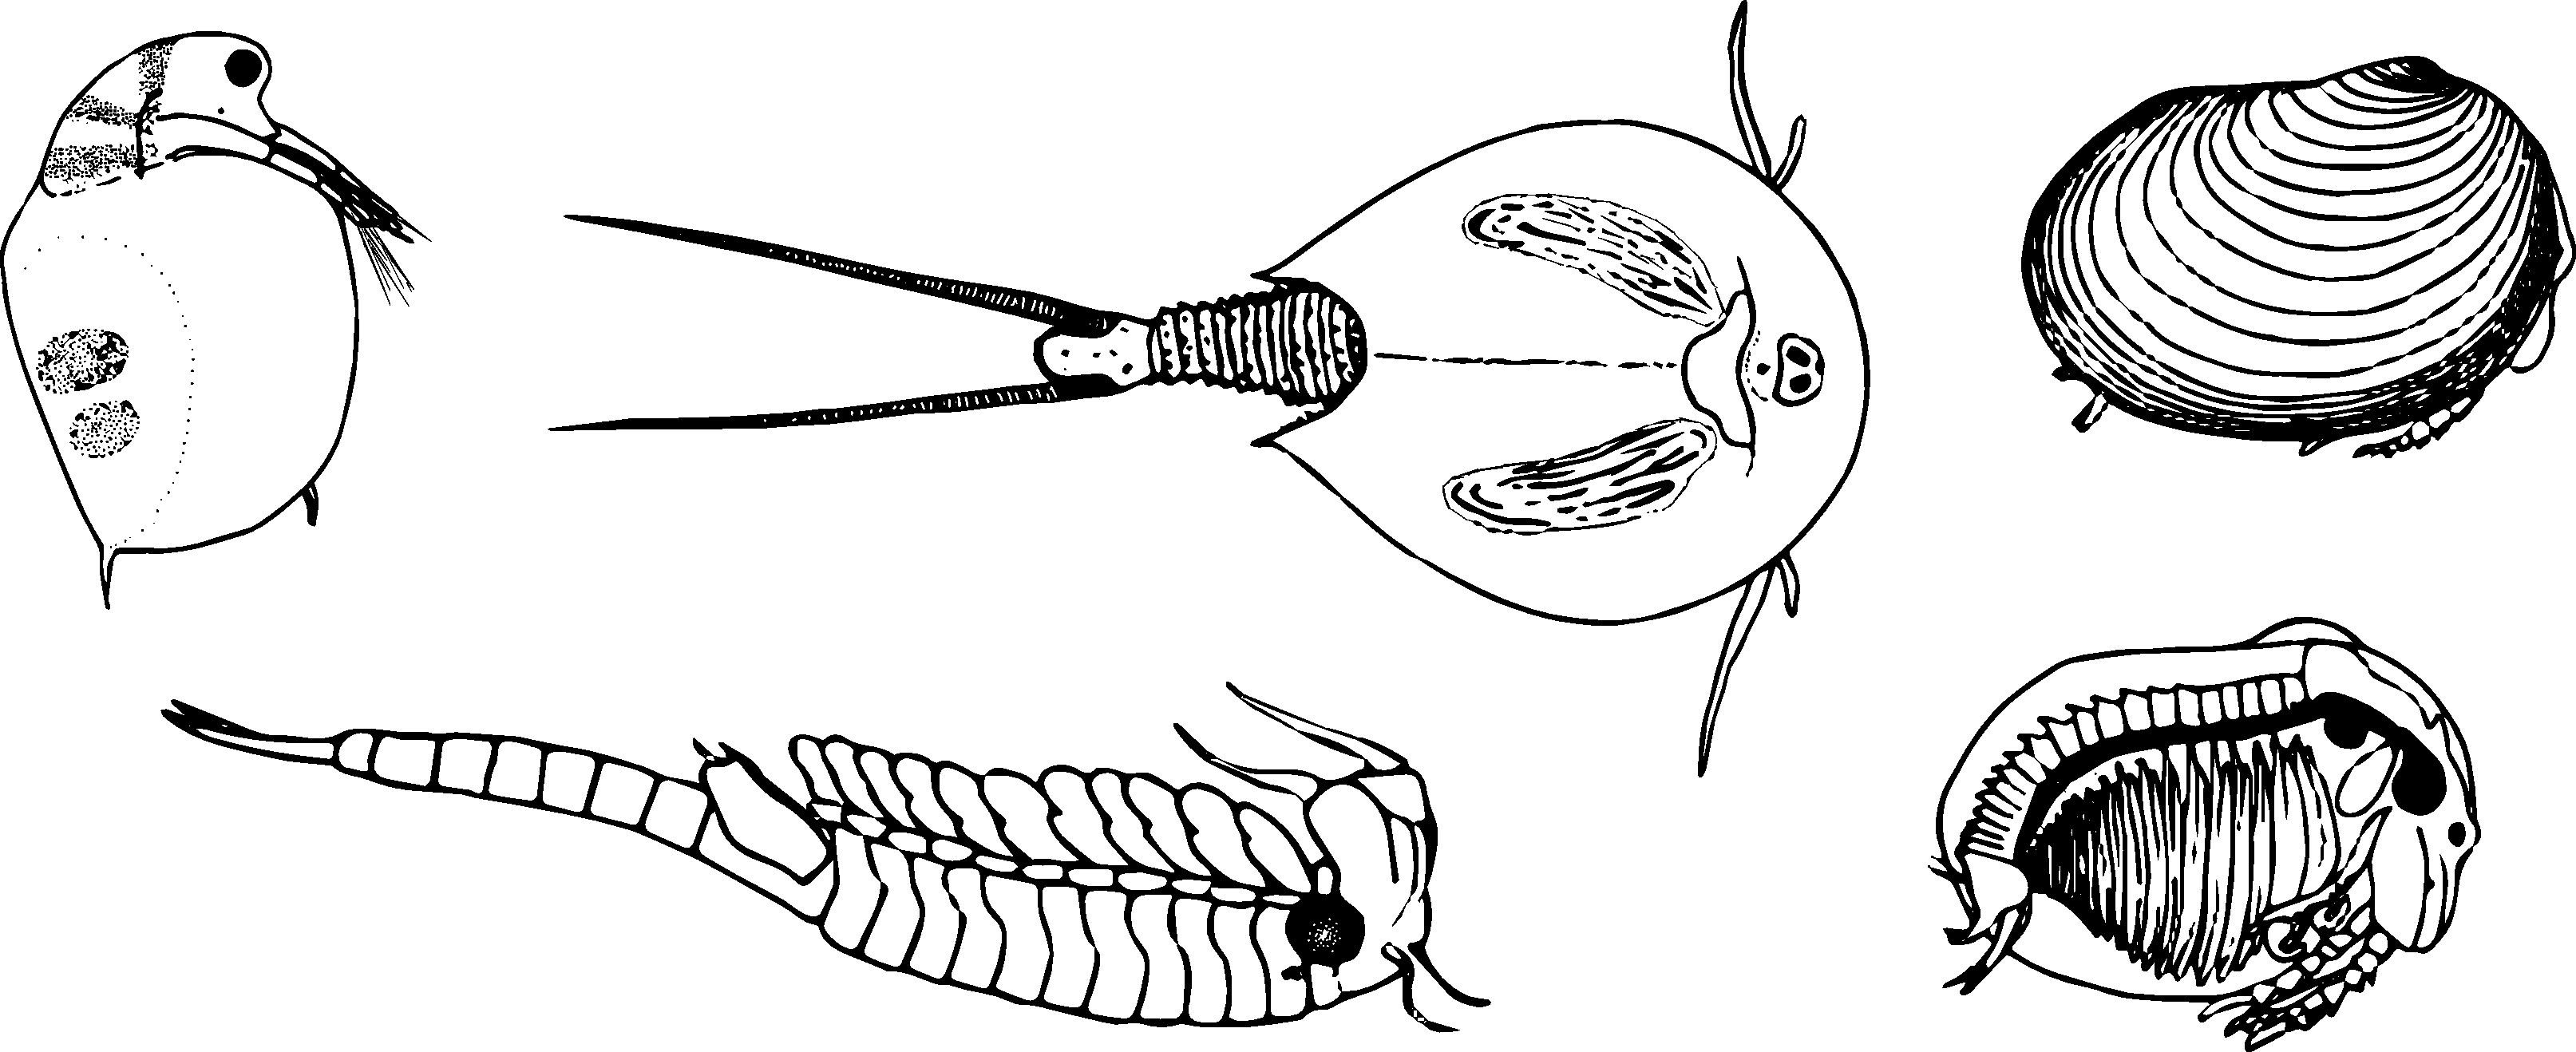
\includegraphics[width=0.8\textwidth]{sections/img/nonhexapod/branchiopoda.pdf}
  \caption{Branchiopoda. redrawn from image at \url{https://web.archive.org/web/20230201062324/https://www.abdn.ac.uk/geosciences/departments/geology/crustaceans-1952.php}}
  \label{fig:branchiopoda}
\end{figure}

\section*{Become a taxonomist}% prob do not need to test on these taxa; could be there simply as demonstrations of the diversity

You've now seen a handful of arthropod taxa, from three groups that are not insects. These organisms are incredibly diverse and remain relevant to understanding the evolution of Arthropoda. Take some time to observe specimens of taxa not covered above, bask in the diversity of their phenotypes, and see if you can classify them correctly. Are they chelicerates, myriapods, or pancrustaceans? Why or why not? Draw and/or describe features you think are diagnostic. Based on their morphology, can you predict their natural history?

\subsubsection*{Solifugae (Solpugida; camelspiders, sunspiders, windscorpions)}\index{Solifugae}
Which major group---Chelicerata, Myriapoda, Pancrustacea---does it belong in and why? What diagnostic characters separate it from the taxa above? What do these arthropods eat, and how do they live?\vspace{3mm}

\begin{figure}[ht!]
  \centering
    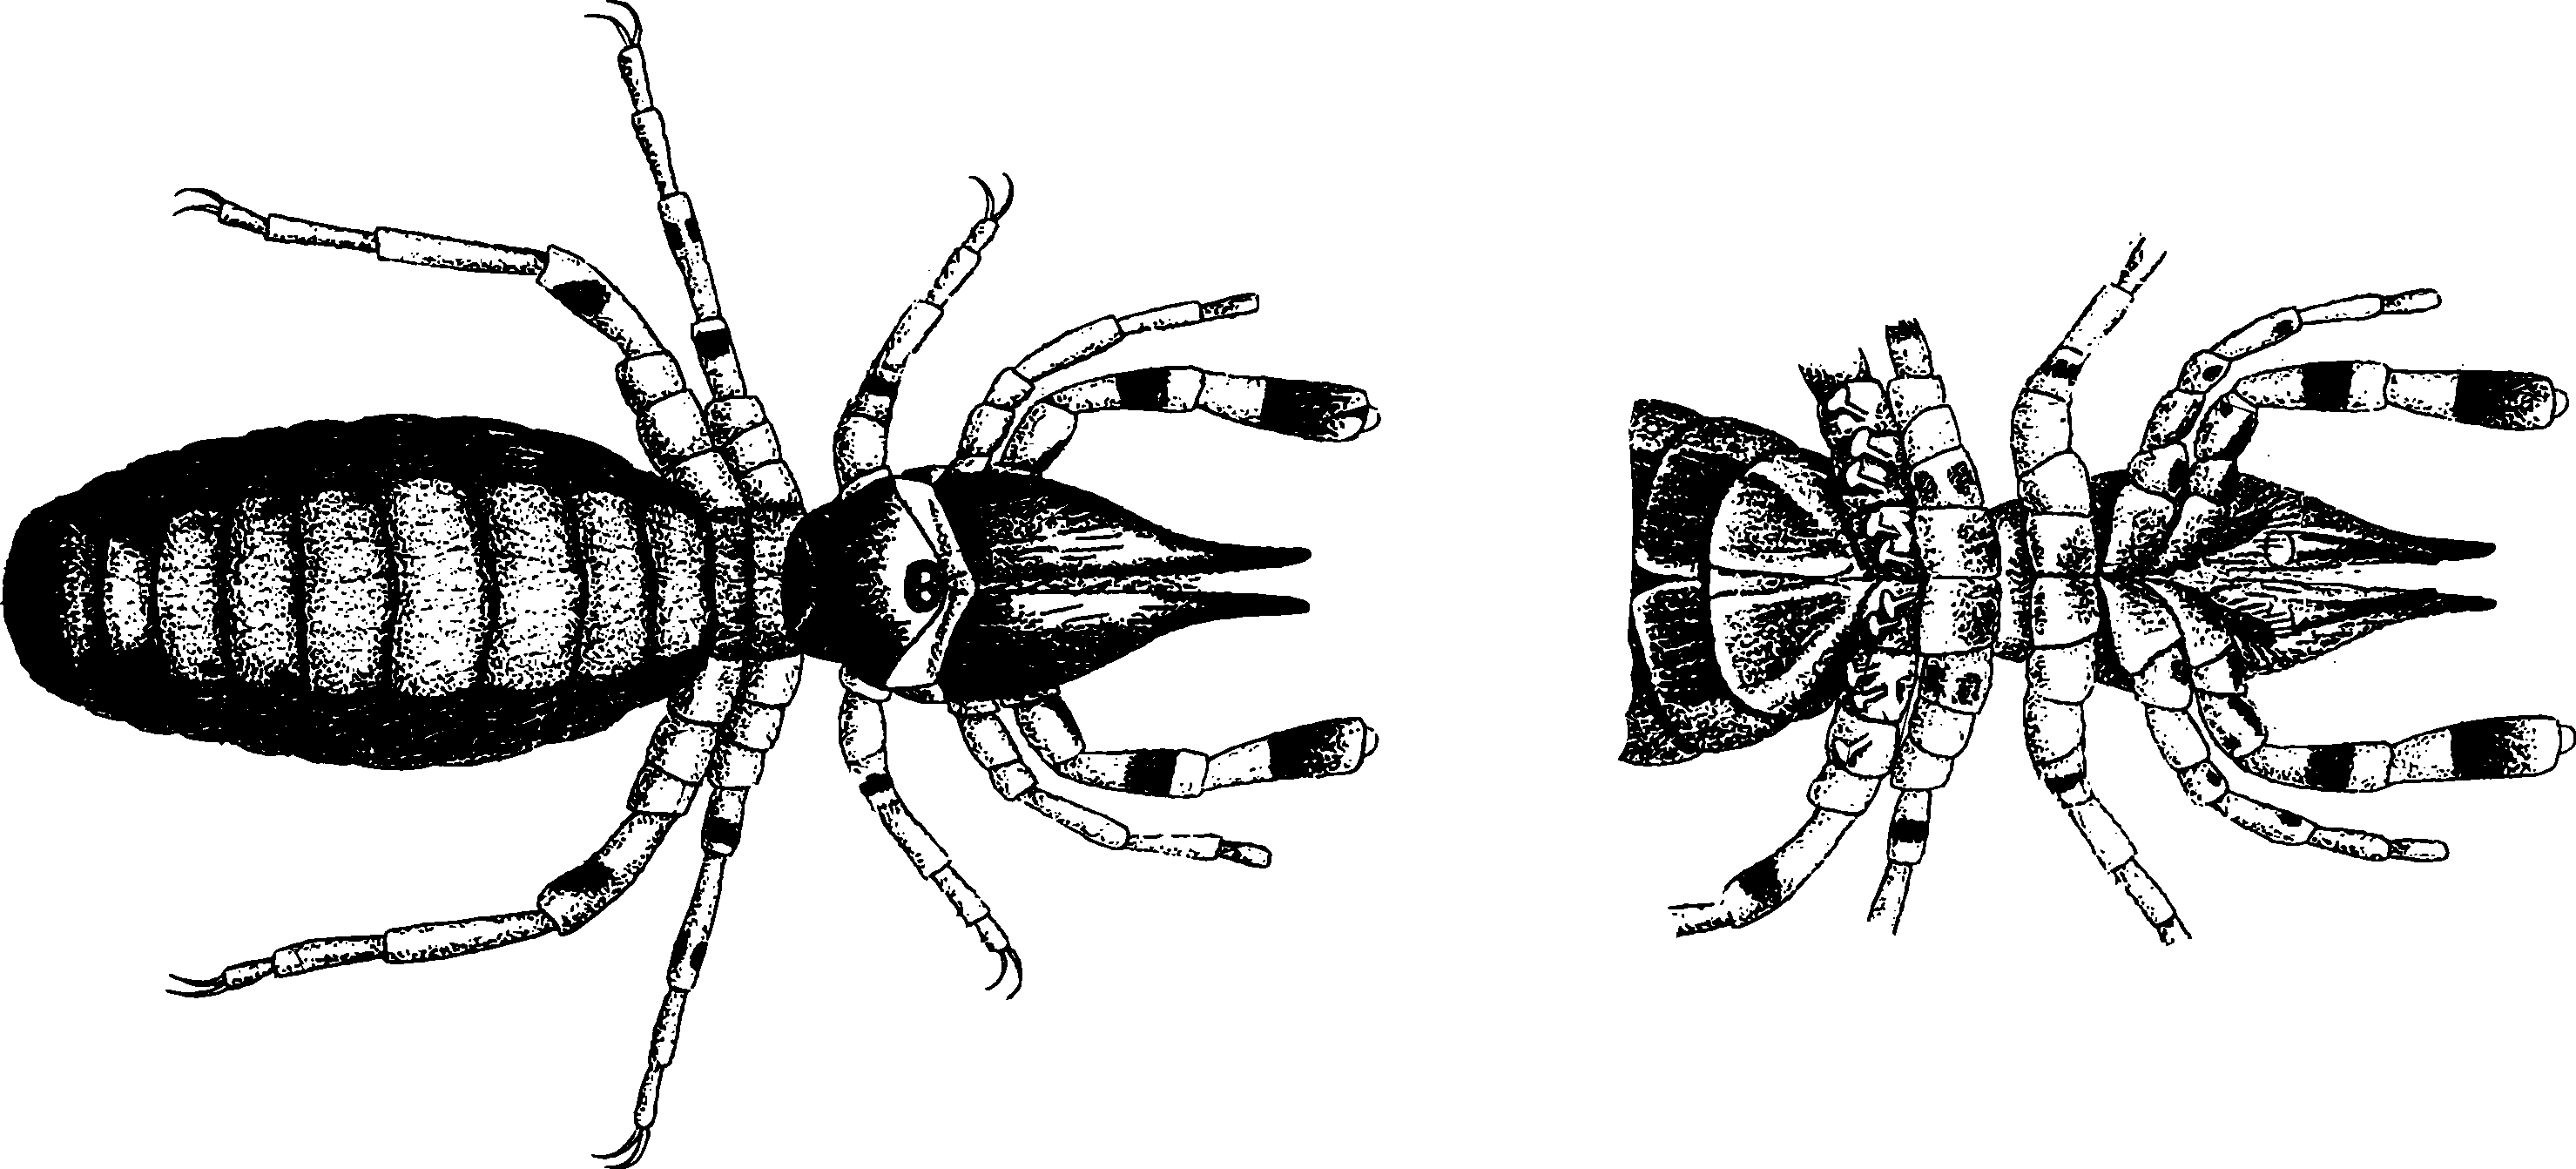
\includegraphics[width=0.8\textwidth]{nonhexapod/solifugae}
  \caption{Solifugae \citep[modified from][Plate 26, Fig. 2]{Bernard1894solifugae}}
  \label{fig:solfugida}
\end{figure}

\subsubsection*{Decapoda (crabs, lobsters, shrimp)}\index{Decapoda}
Which major group does it belong in and why? What diagnostic characters separate it from other taxa in the same group? What do these arthropods eat, and how do they live?\vspace{3mm}

\begin{figure}[ht!]
  \centering
    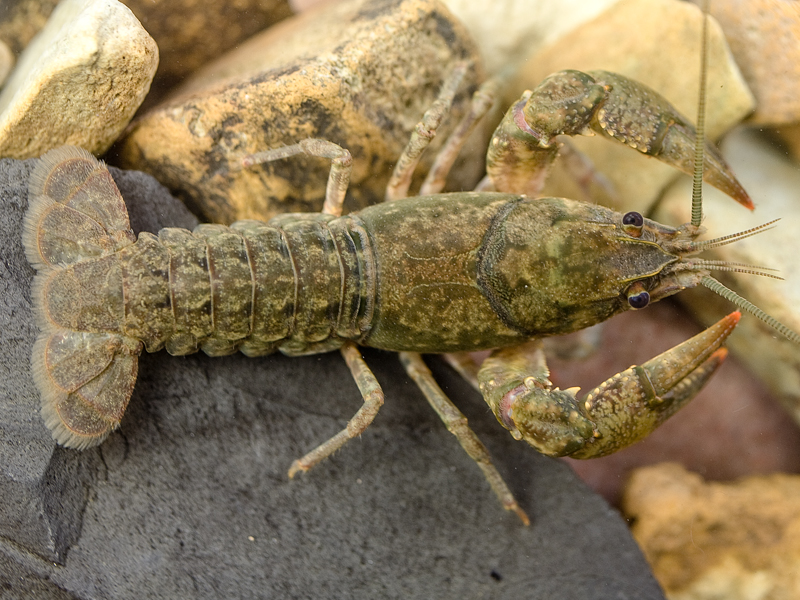
\includegraphics[width=0.6\textwidth]{nonhexapod/decapod}
  \caption{Decapoda \citep[][Plate VII]{bhlitem114131}}
  \label{fig:decapoda}
\end{figure}

\subsubsection*{Thelyphonida (Uropygi, Uropygida, vinegaroons, whipscorpions)}\index{Thelyphonida}
Which major group does it belong in and why? What diagnostic characters separate it from the other taxa in that group? See figure \ref{fig:thelyphonida}. What do these arthropods eat, and how do they live?\vspace{3mm}

\begin{figure}[ht!]
  \centering
    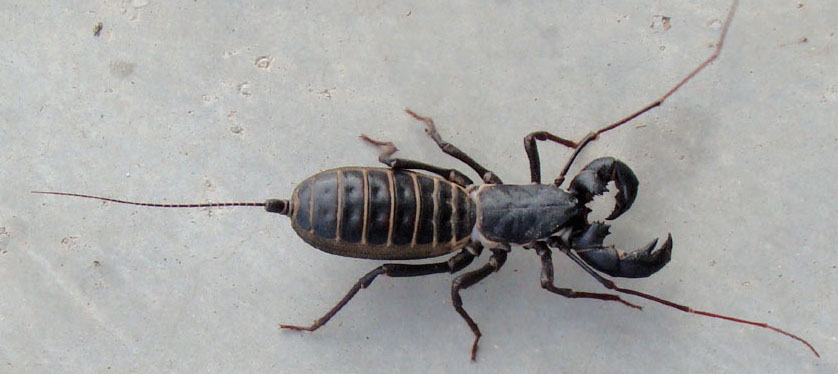
\includegraphics[width=0.5\textwidth]{nonhexapod/thelyphonida}
  \caption{Thelyphonida \citep[][Fig. 57]{bhlitem40112britmus}}
  \label{fig:thelyphonida}
\end{figure}

\subsubsection*{Amblypygi (tail-less whipscorpions)}\index{Amblypygi}
Which major group does it belong in and why? What diagnostic characters separate it from other taxa in that group? See figure \ref{fig:ambly1}. What do these arthropods eat, and how do they live?\vspace{3mm}

\begin{figure}[ht!]
  \centering
    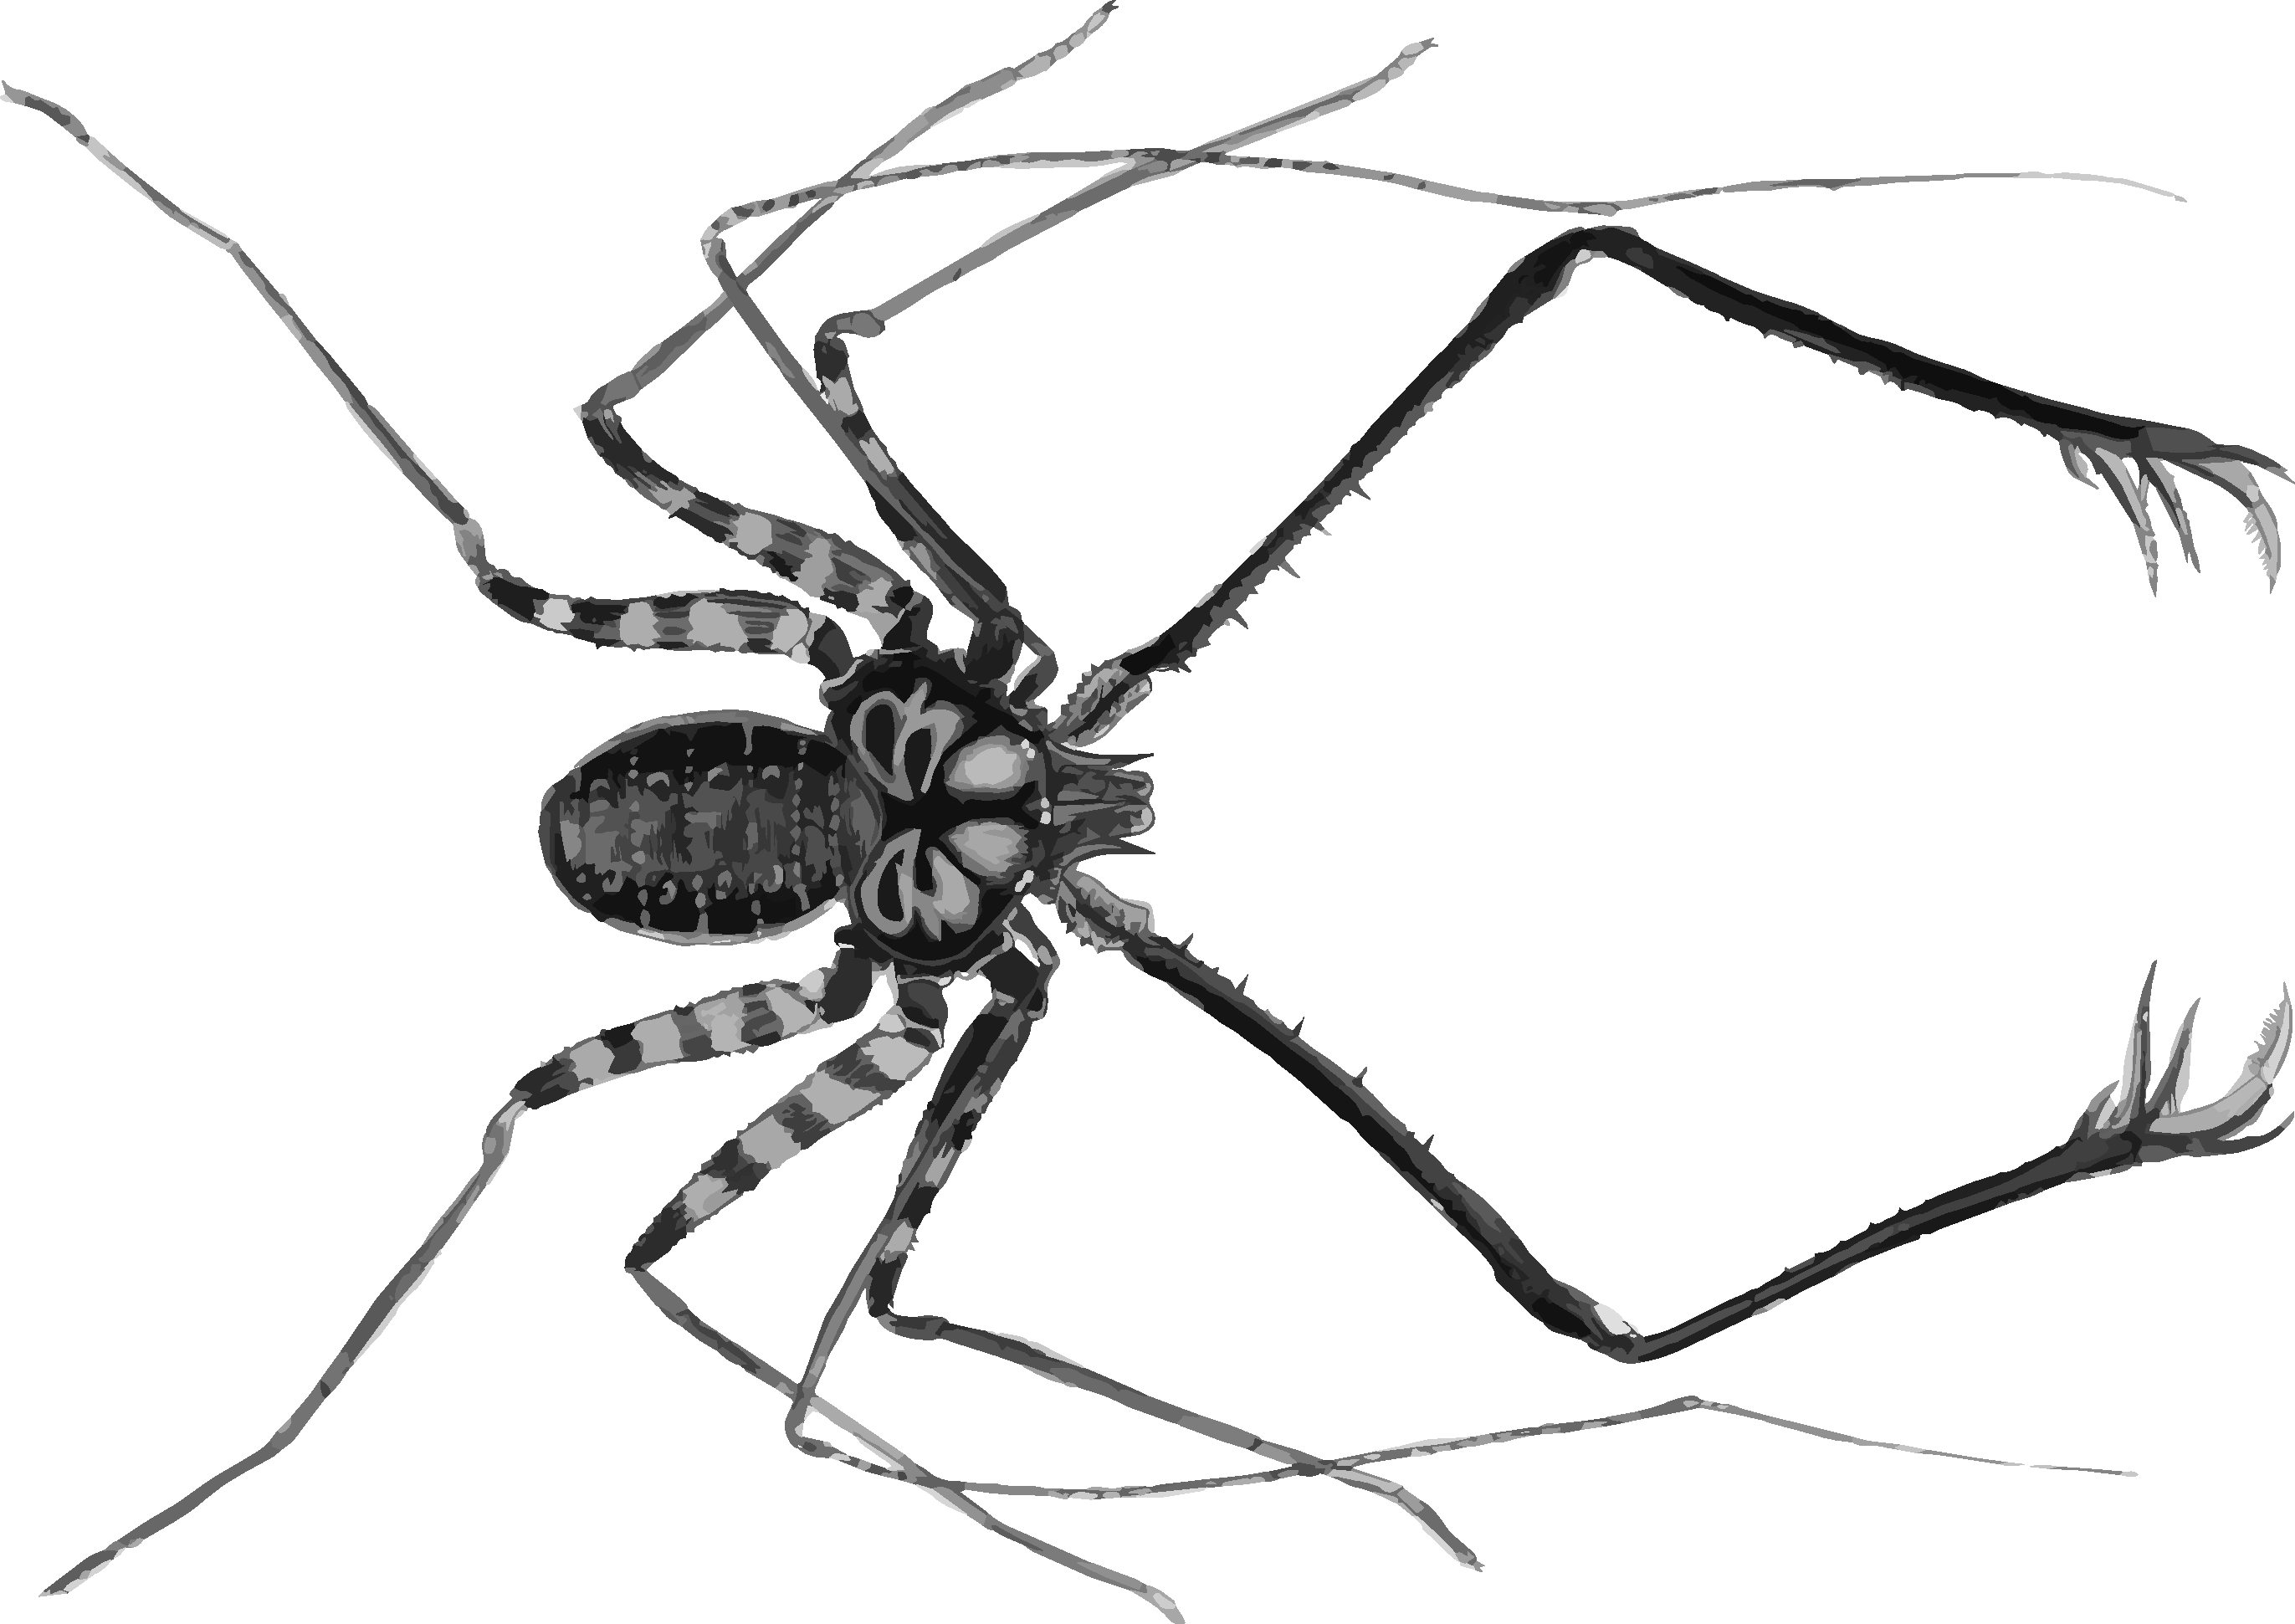
\includegraphics[width=0.55\textwidth]{nonhexapod/amblypygi}
  \caption{Amblypygi \citep[][plate CCCXXXVI]{bhlitem55834arach}}
  \label{fig:ambly1}
\end{figure}

\subsubsection*{Symphyla (symphylans)}\index{Symphyla}
Which major group does it belong in and why? What diagnostic characters separate it from the taxa above? What do these arthropods eat, and how do they live?\vspace{3mm}

\begin{figure}[ht!]
  \centering
    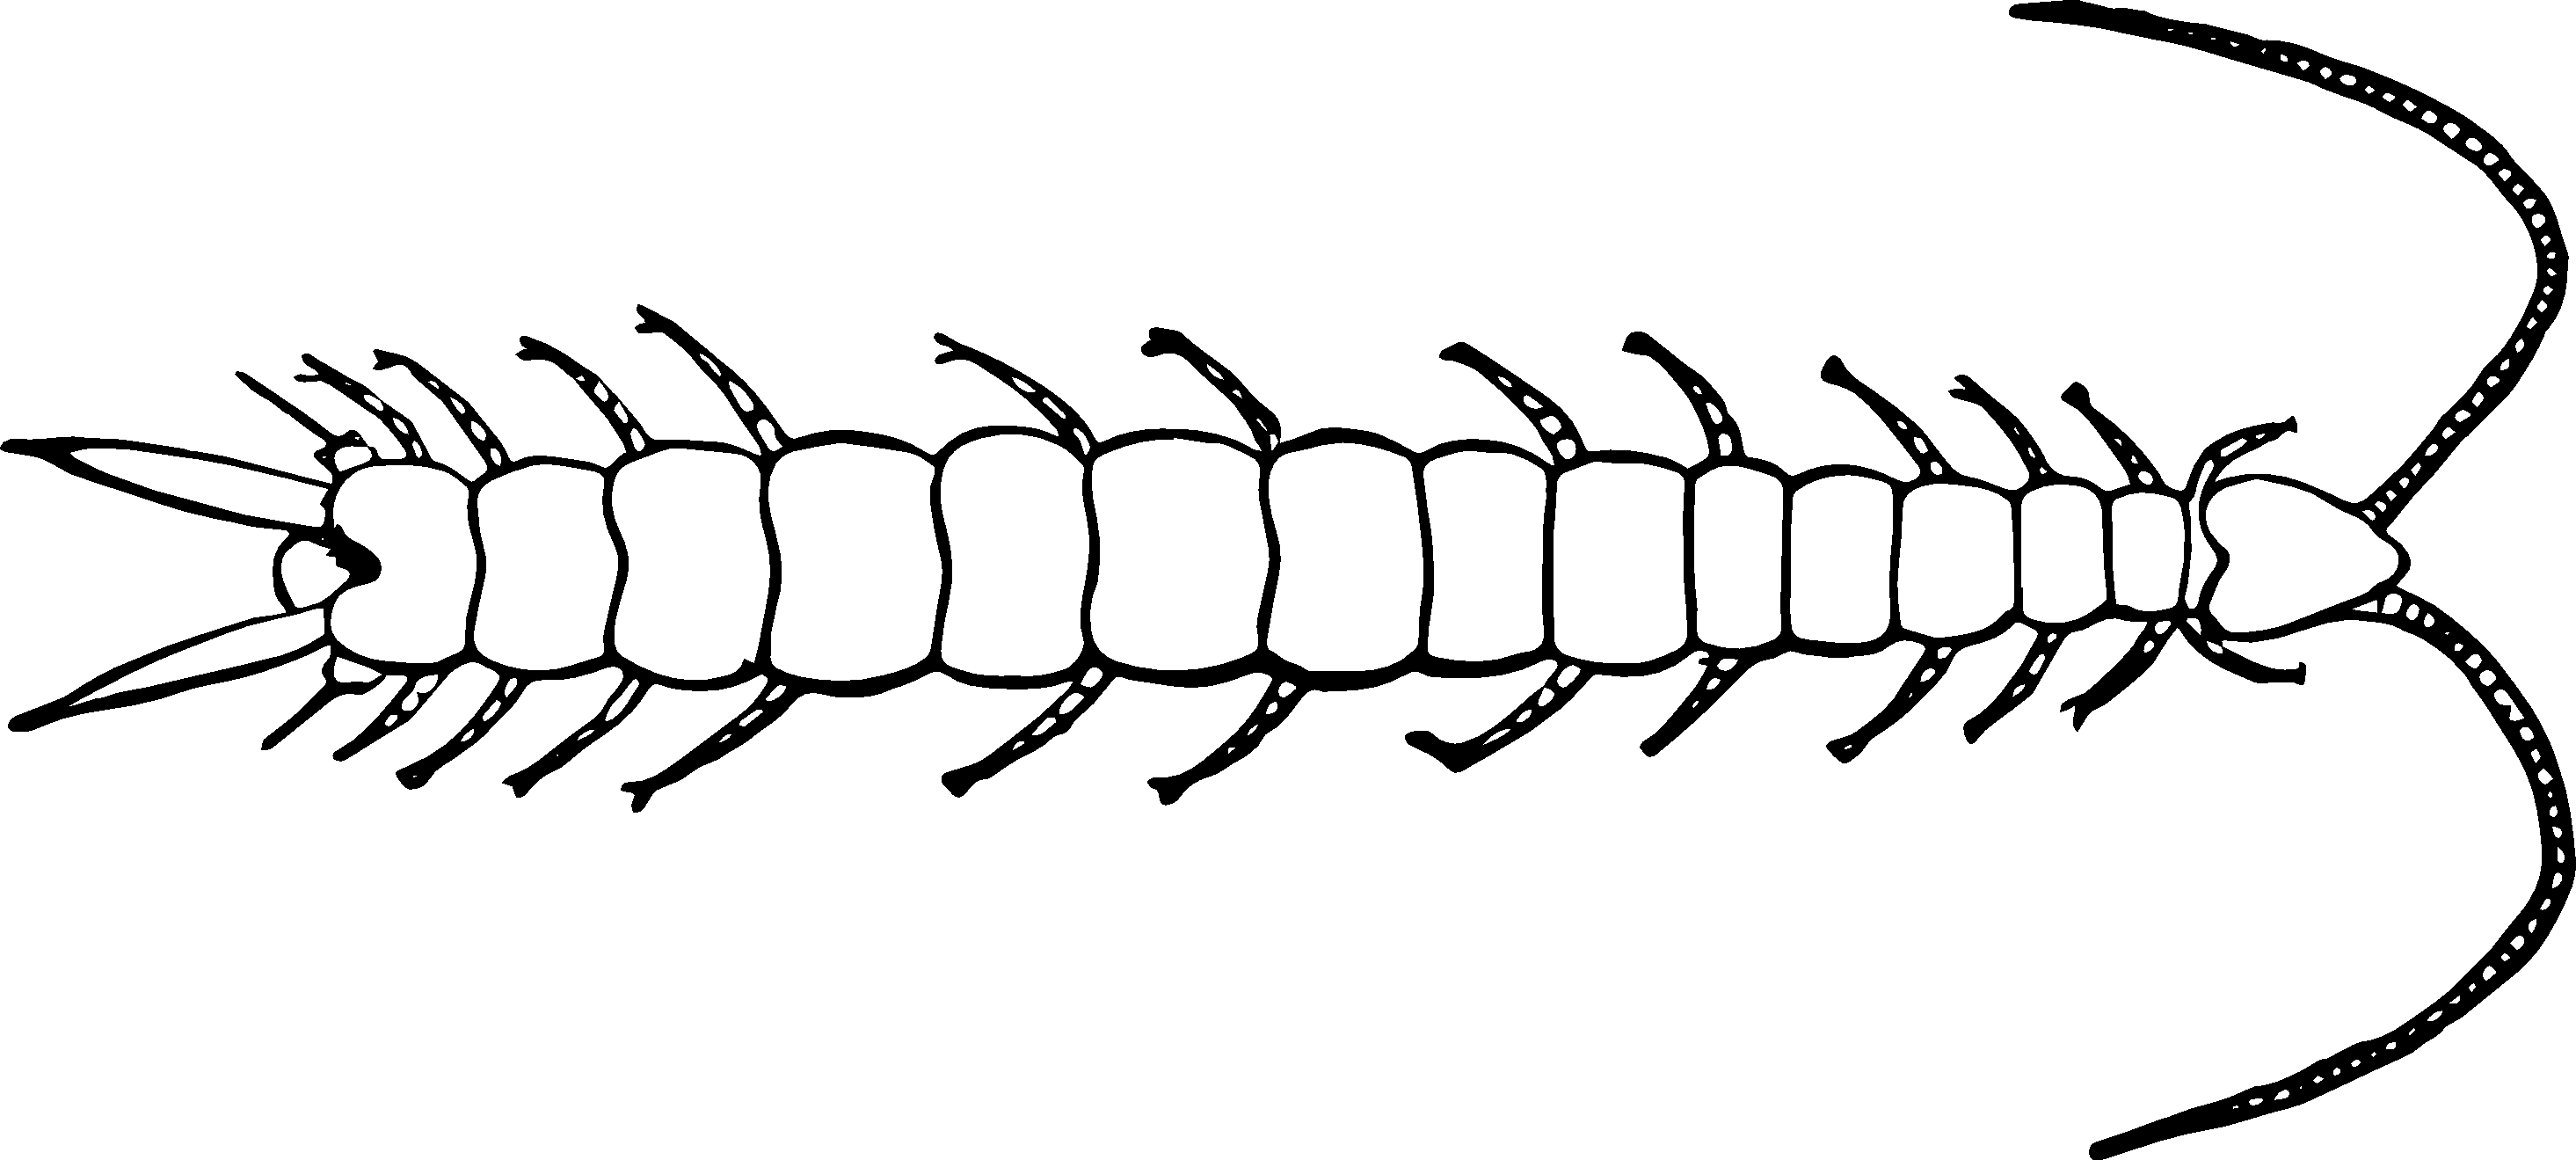
\includegraphics[width=0.55\textwidth]{nonhexapod/symphyla}
  \caption{Symphyla \citep[][Fig. 14B]{bhlitem16837entom}}
  \label{fig:symphyla}
\end{figure}

\section*{Test yourself}

\noindent{}Can you draw a phylogeny showing the relationships between Onychophora, Chelicerata, Myriapoda, and Pancrustacea (including Hexapoda)? Which node is the common ancestor of Arthropoda? \citep[Hint: see][]{Dunlop2013}\vspace{3mm}

\noindent{}Why are some of these taxa \textit{orders of magnitude} more diverse than others? For example, Araneae has at least 50,000 named species, whereas Amblypygi has merely 150 or so species. Diplopoda is comprised of \textit{thousands} of species, whereas Symphyla has merely 250 or so.

\clearpage
\thispagestyle{empty}


\chapter{Non-pterygote Hexapoda}
\section*{Introduction}\index{Hexapoda}
Here we begin looking at taxa classified in \textbf{Hexapoda}. In most cases you will examine multiple families, most of which you will be tested on in lab practicals. You may be shown more families than are in this manual---primarily so that you can better grasp the diversity that exists---but you will not have to sight-identify these other families. Looking at these other families may help to you, though, in identifying specimens for your collection. Some characters might be impossible to see, given the equipment and specimens we have in lab, but they are provided for future reference.

\section{Hexapoda}

\begin{itemize}
\item 3 tagmata present: head, thorax, abdomen
\item 3 pairs of uniramous thoracic appendages (legs) present
\end{itemize}

\section*{Entognatha}\index{Entognatha}

\begin{itemize}
\item Antennae, when present, truly segmented (\textit{i.e.}, each segment has intrinsic musculature; see figure \ref{fig:dipluraAntenna})
\item Mouthpart concealed externally (figure \ref{fig:proturans}, left)
\item Tarsus not subdivided into tarsomeres (figure \ref{fig:proturans}, right)
\end{itemize}

\begin{figure}[ht!]
    \centering
    \begin{subfigure}[ht!]{0.2\textwidth}
        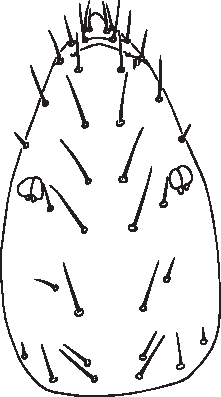
\includegraphics[width=\textwidth]{nonpterygote/proturanHead}
        \caption{}
        \end{subfigure}
    \hfill
    \begin{subfigure}[ht!]{0.12\textwidth}
        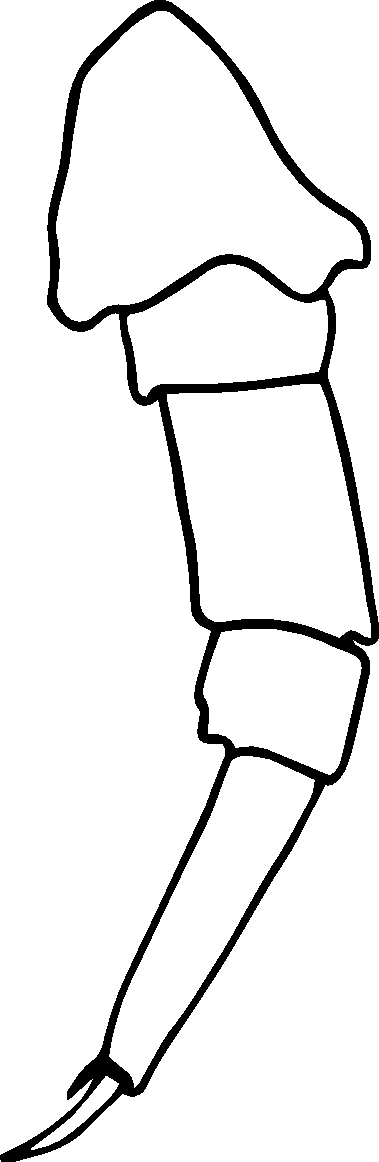
\includegraphics[width=\textwidth]{nonpterygote/proturanLeg}
        \caption{}
    \end{subfigure}
    \caption{Protura. \textbf{(a)} Head in dorsal view, with pseudoculi \citep[][Fig. 1A]{Yun2016}; \textbf{(b)} Leg \cite[redrawn from][Fig. 12]{bhlpart35427}}\label{fig:proturans}
\end{figure}

\subsection{Protura (coneheads)}\index{Protura}
\noindent{}\textit{Diagnostic characters:} Antennae apparently absent (figure \ref{fig:proturanhab}); eyes absent; sensory organs (pseudoculi) present where one would expect eyes or antennae to be; mandibles without molar area (proximal flattened region for grinding food); body very small (\textless1.5 mm long); abdomen 11-segmented in mature specimens, cerci absent.\vspace{3mm}

\noindent{}\textit{Natural History:} Proturans can be abundant in leaf litter and soil samples, but they are incredibly small and usually overlooked. More than 800 species have been described worldwide, and most are smaller than 1 mm.\vspace{3mm}

\begin{theo}
{}How might the absence of antennae be adaptive for these hexapods? Which structure functions as the primary anterior sensory appendage? \end{theo}\vspace{3mm}

\begin{figure}[ht!]
  \centering
    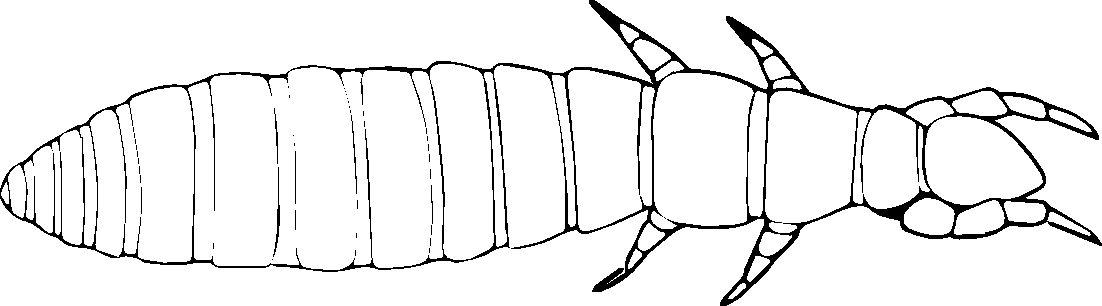
\includegraphics[width=0.55\textwidth]{nonpterygote/proturaHabitus}
  \caption{Protura habitus (illustration by Laura Porturas, Penn State)}
  \label{fig:proturanhab}
\end{figure}

\subsection{Diplura (diplurans)}\index{Diplura}
\noindent{}\textit{Diagnostic characters:} Antennae filiform; eyes absent; pseudoculi absent; mandibles without molar area; body usually \textgreater3 mm long; cerci distinct; abdominal segments often with styli.\vspace{3mm}

\noindent{}\textit{Natural History:} These hexapods are quite common, especially under rocks and logs, at the interface between leaf litter and soil. Like Protura, there are approximately 800 species known worldwide, but diplurans are generally much larger (up to 5 mm long in North America and up to 5 cm in the tropics).\vspace{3mm}

\begin{theo}
{}Compare \textbf{Japygidae} (figure \ref{fig:japygidhab}) to \textbf{Campodeidae} (figure \ref{fig:campodeidhab}). What is your hypothesis for why the cerci vary phenotypically between families? What is their function?\end{theo}

\begin{figure}[ht!]
  \centering
    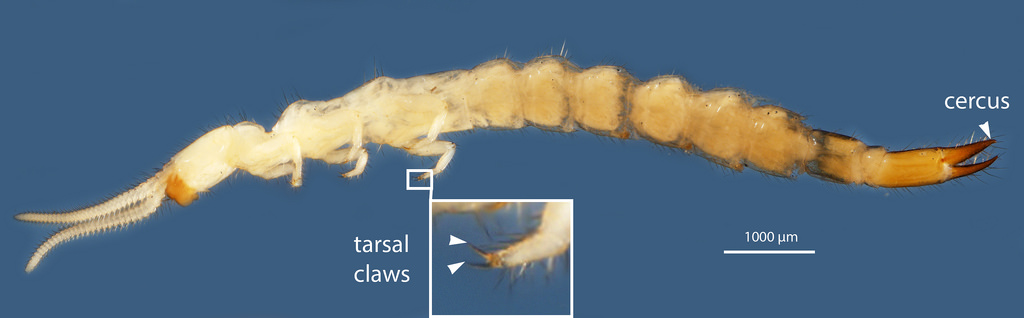
\includegraphics[width=0.6\textwidth]{nonpterygote/japygid1}
  \caption{Japygidae dorsal habitus (illustration by Laura Porturas, Penn State)}
  \label{fig:japygidhab}
\end{figure}
\begin{figure}[ht!]
  \centering
    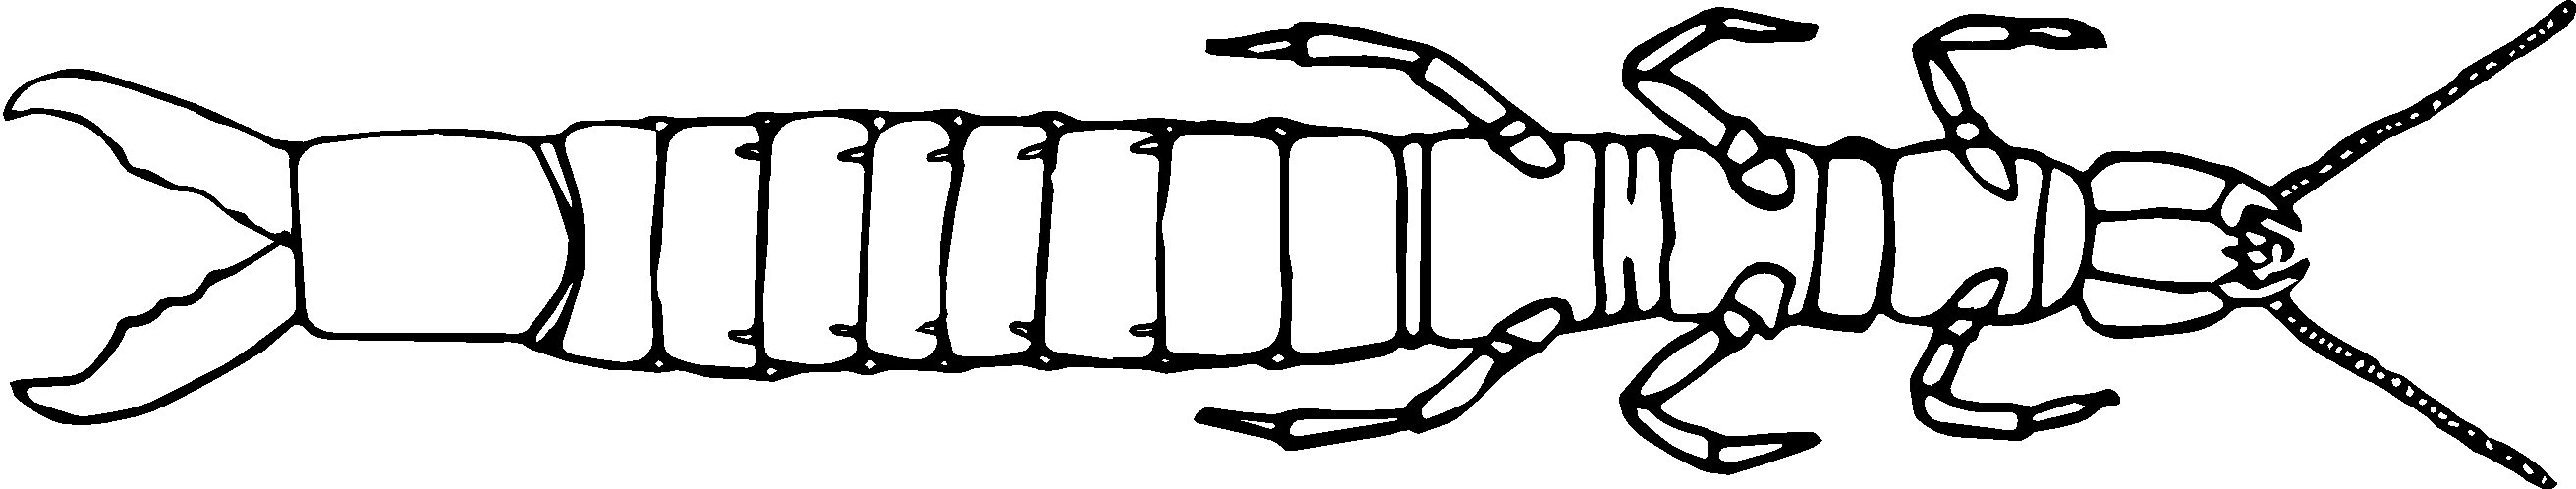
\includegraphics[width=0.6\textwidth]{nonpterygote/DipluraVentral}
  \caption{Japygidae ventral habitus \citep[redrawn from][Fig. 8]{bhlitem30465Insects}}
  \label{fig:japygidhabvent}
\end{figure}

\begin{figure}[ht!]
  \centering
    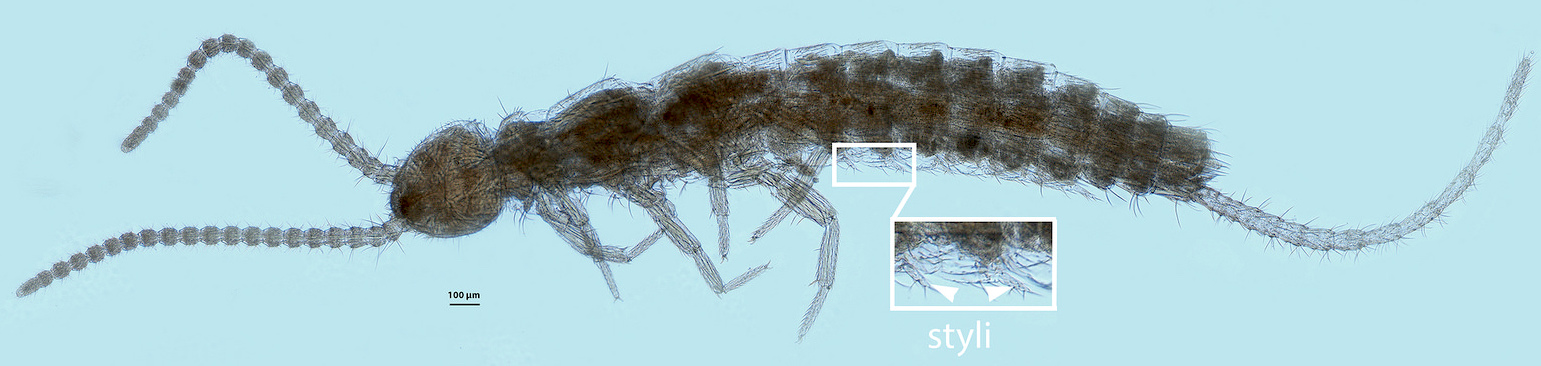
\includegraphics[angle=270,width=0.6\textwidth]{nonpterygote/campodeid1}
  \caption{Campodeidae habitus (illustration by Laura Porturas, Penn State)}
  \label{fig:campodeidhab}
\end{figure}

\begin{figure}[ht!]
  \centering
    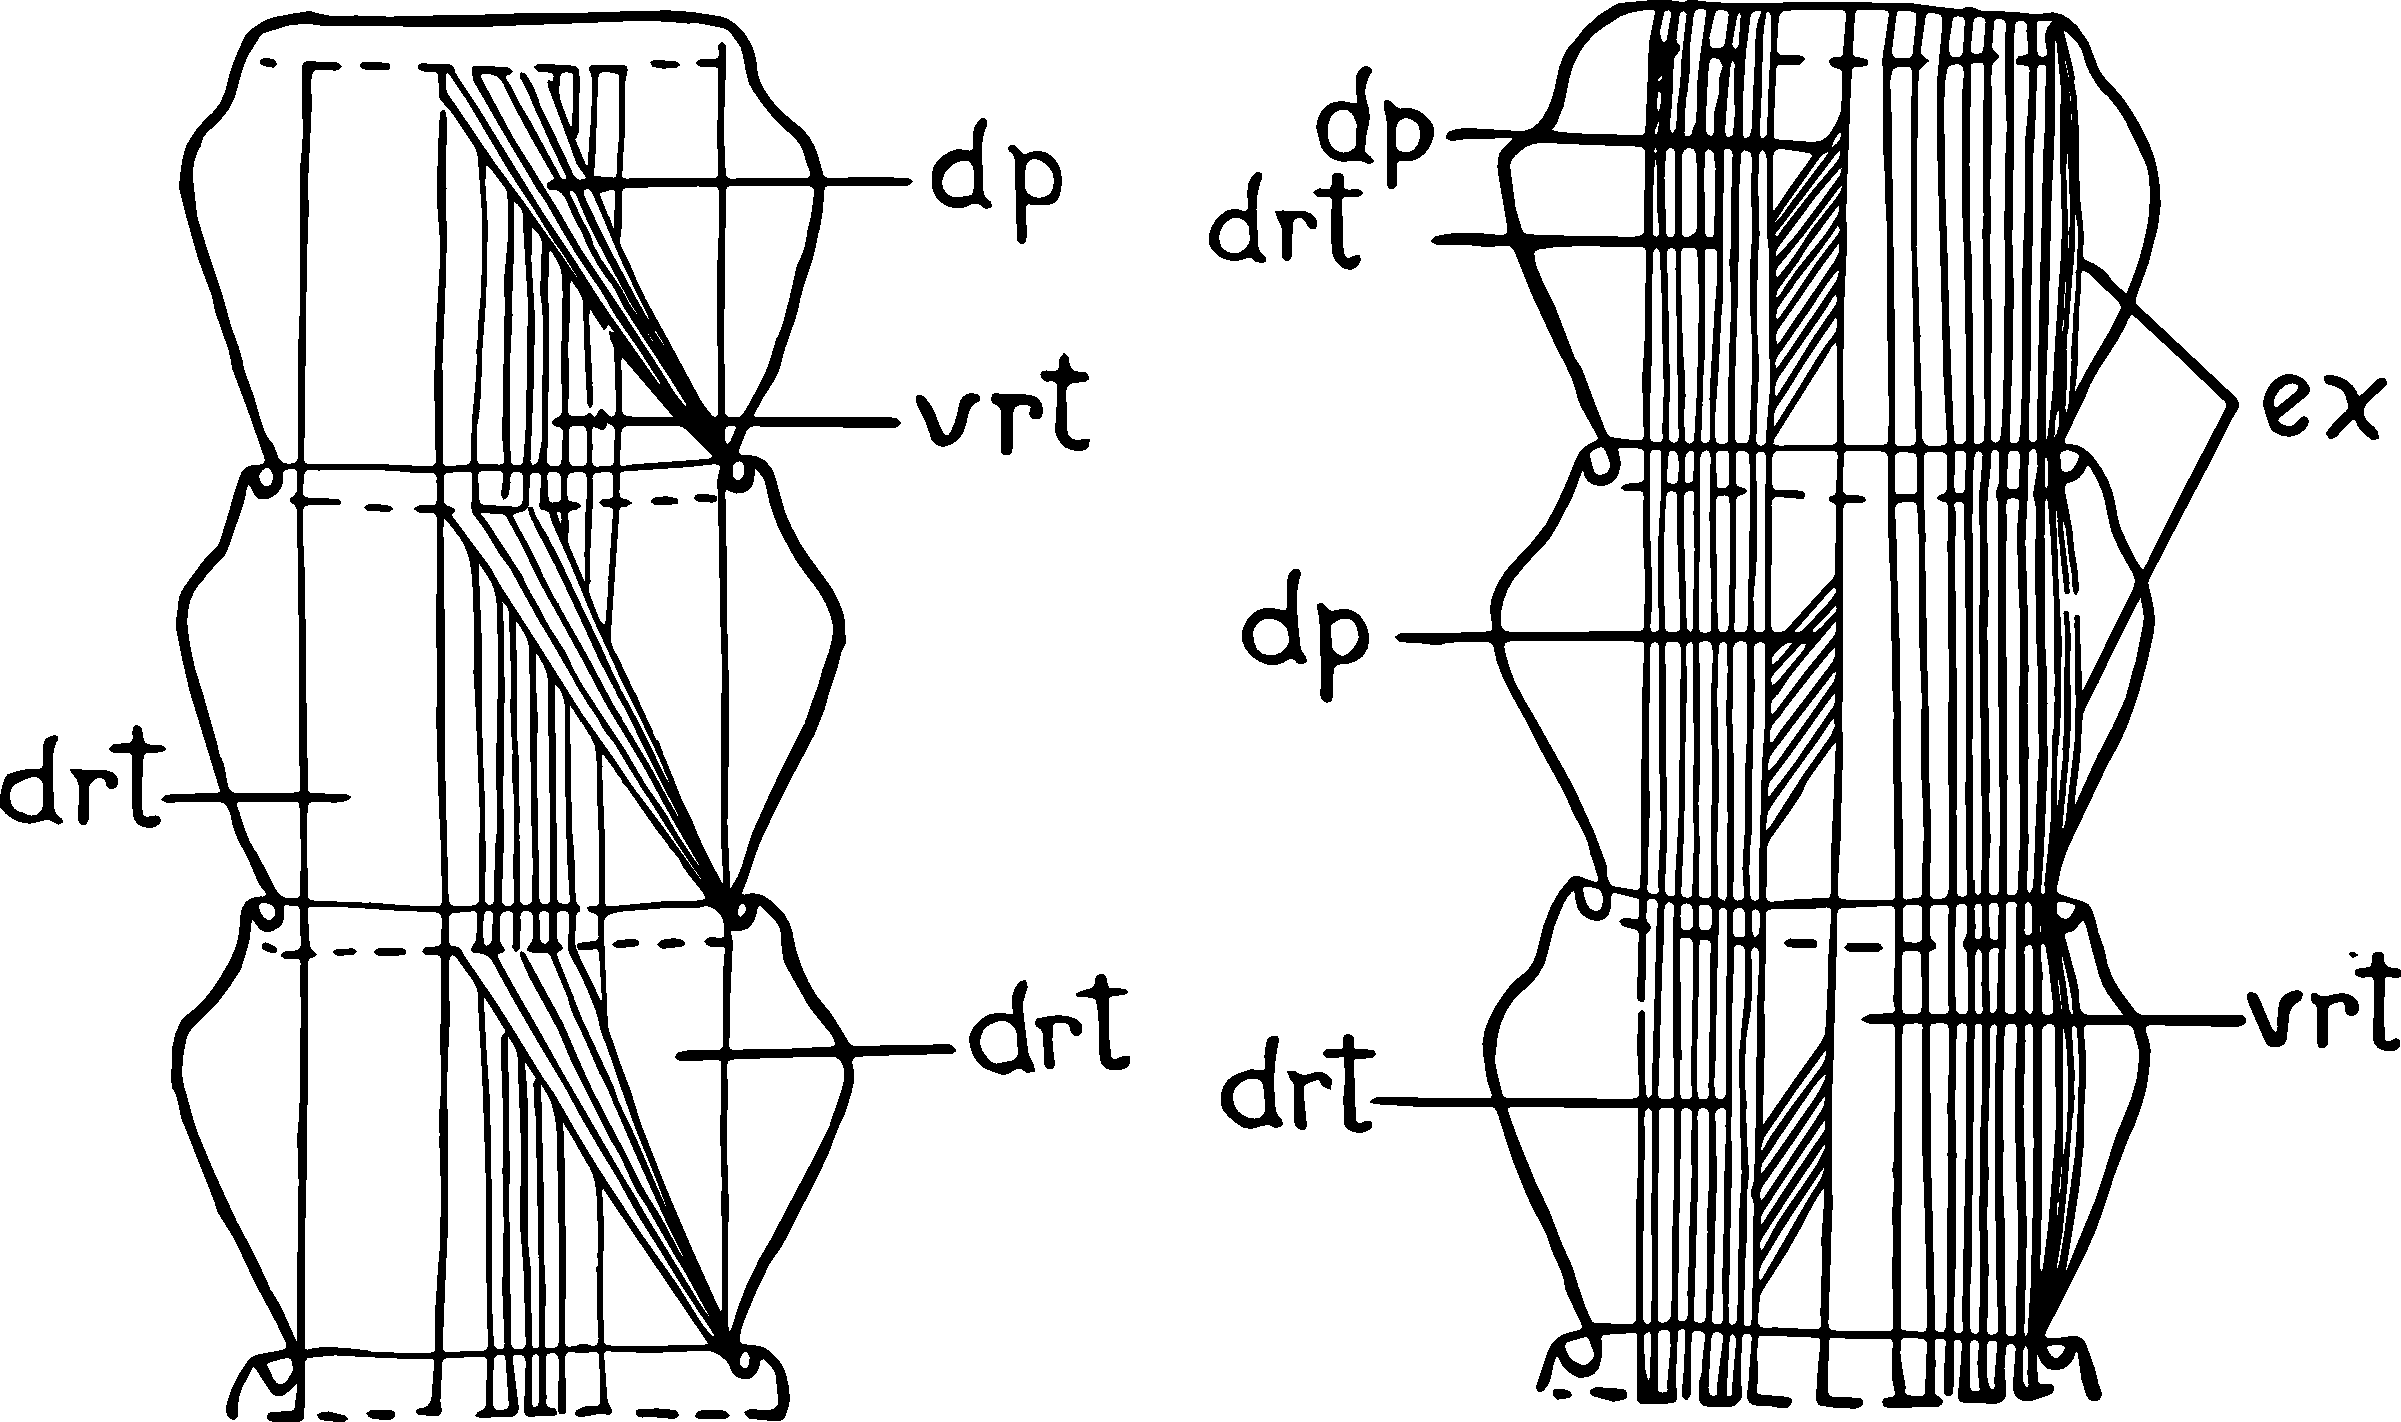
\includegraphics[width=0.5\textwidth]{nonpterygote/dipluraAntenna}
  \caption{Diplura antenna. Antennal segments VIII to X of a species of \textit{Japyx}; left, ventral view; right, dorsal view; dp, depressor muscle; drt, dorsal retractor muscle; ex, extensors; vrt, ventral retractor muscle \citep[redrawn from][Fig. 2]{bhlpart81512}}
  \label{fig:dipluraAntenna}
\end{figure}

\subsection{Collembola (springtails)}\index{Collembola}
Collembola are commonly referred to as ``springtails'' for their ability to jump using a structure called a \latinword{furculum}. We will focus on higher-level taxa, which are usually ranked as orders: Symphypleona, Poduromorpha, Entomobryomorpha. Collembola can be recognized by the following traits:

\begin{itemize}
\item Compound eyes present
\item mandibles with molar area
\item antennae usually $\leq$4 segments
\item tibia fused with tarsus (tibiotarsus)
\item abdomen with $\leq$6 segments: 1st segment with ventral tube (collophore), 3rd abdominal segment modified ventrally (retinaculum) to receive furculum, 5th abdominal segment with forked structure (furculum), usually folded under abdomen
\item body length usually 1--3 mm
\end{itemize}

\subsubsection{Symphypleona (globular springtails)}\index{Symphypleona}
\noindent{}\textit{Diagnostic characters:} Head typically hypognathous, anteroposteriorly flattened; antennae longer than head; prothorax indistinct dorsally, narrowly articulated with head; several abdominal segments fused dorsally.\vspace{3mm}

\noindent{}\textit{Natural History:} Biologically diverse. Symphypleona is subdivided into about 10 families. Some species are semiaquatic.\vspace{3mm}

\begin{figure}[ht!]
  \centering
    \reflectbox{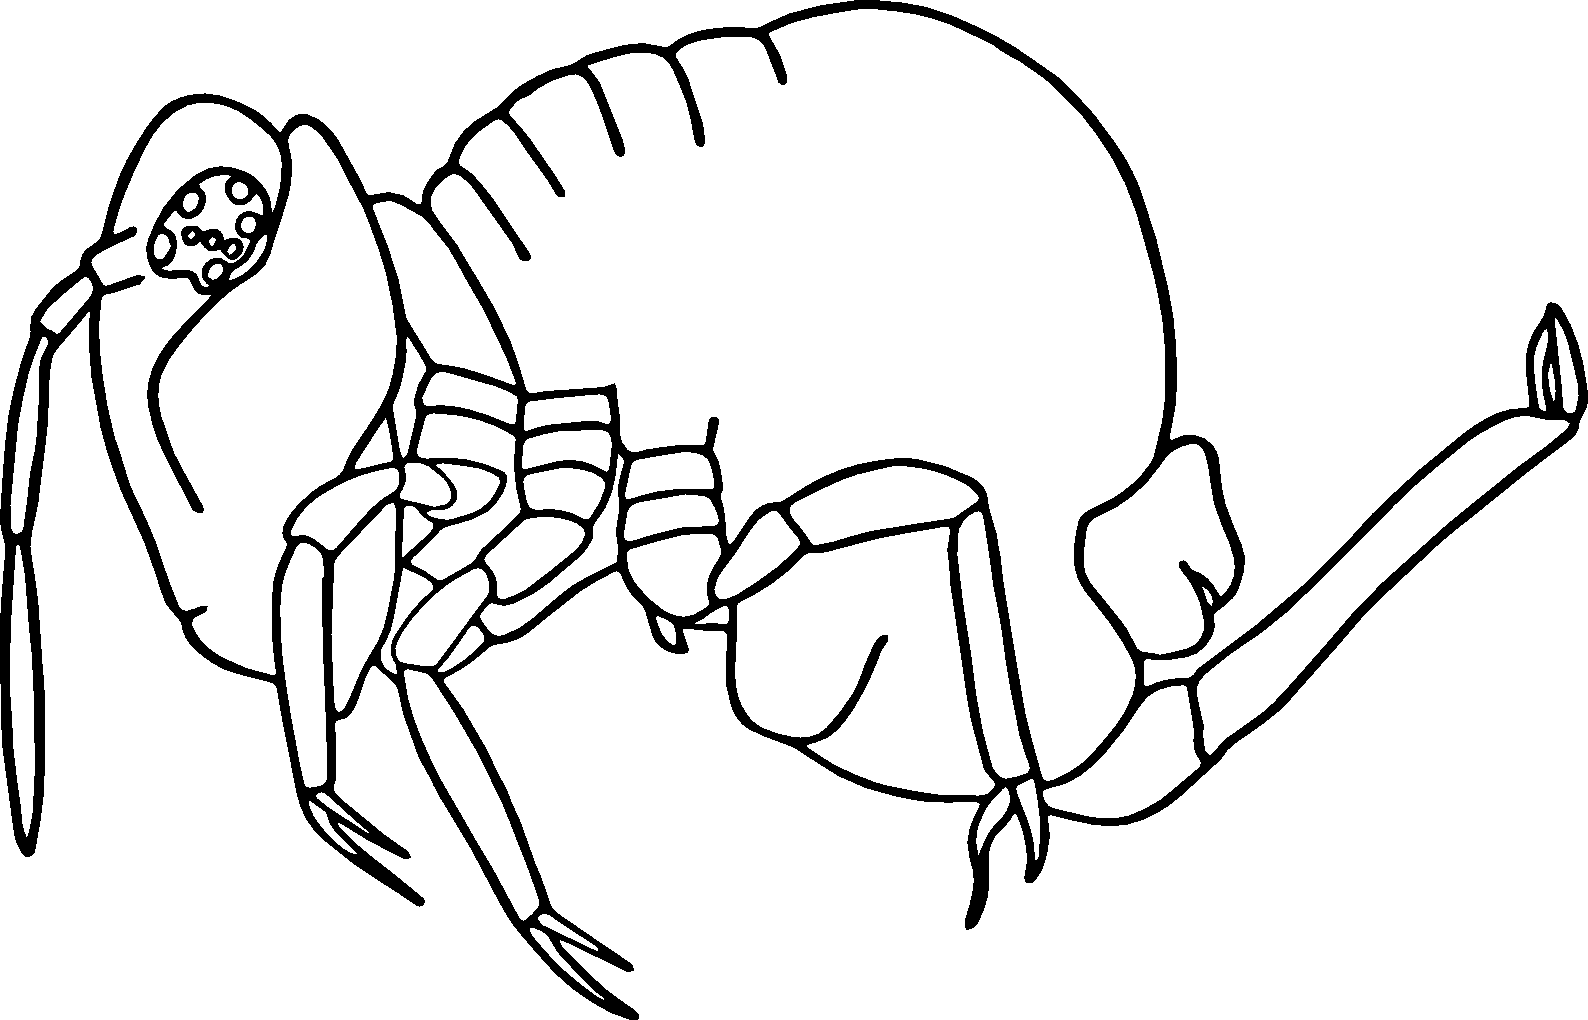
\includegraphics[width=0.4\textwidth]{nonpterygote/sminthuridHabitus}}
  \caption{Symphypleona (Sminthuridae) habitus \citep[redrawn from][Fig. 19]{bhlitem30465Insects}}
  \label{fig:sminthhab}
\end{figure}

\subsubsection{Poduromorpha}\index{Poduromorpha}
\noindent{}\textit{Diagnostic characters:} Head typically prognathous, not anteroposteriorly flattened; antennae usually shorter than head; prothorax distinct dorsally, broadly articulated with head; legs relatively short; abdominal segments 2--4 not fused.\vspace{3mm}

\noindent{}\textit{Natural History:} Like Symphypleona, these hexapods are biologically diverse, with many semiaquatic species. There are also about 10 families.\vspace{3mm}

\begin{figure}[ht!]
  \centering
    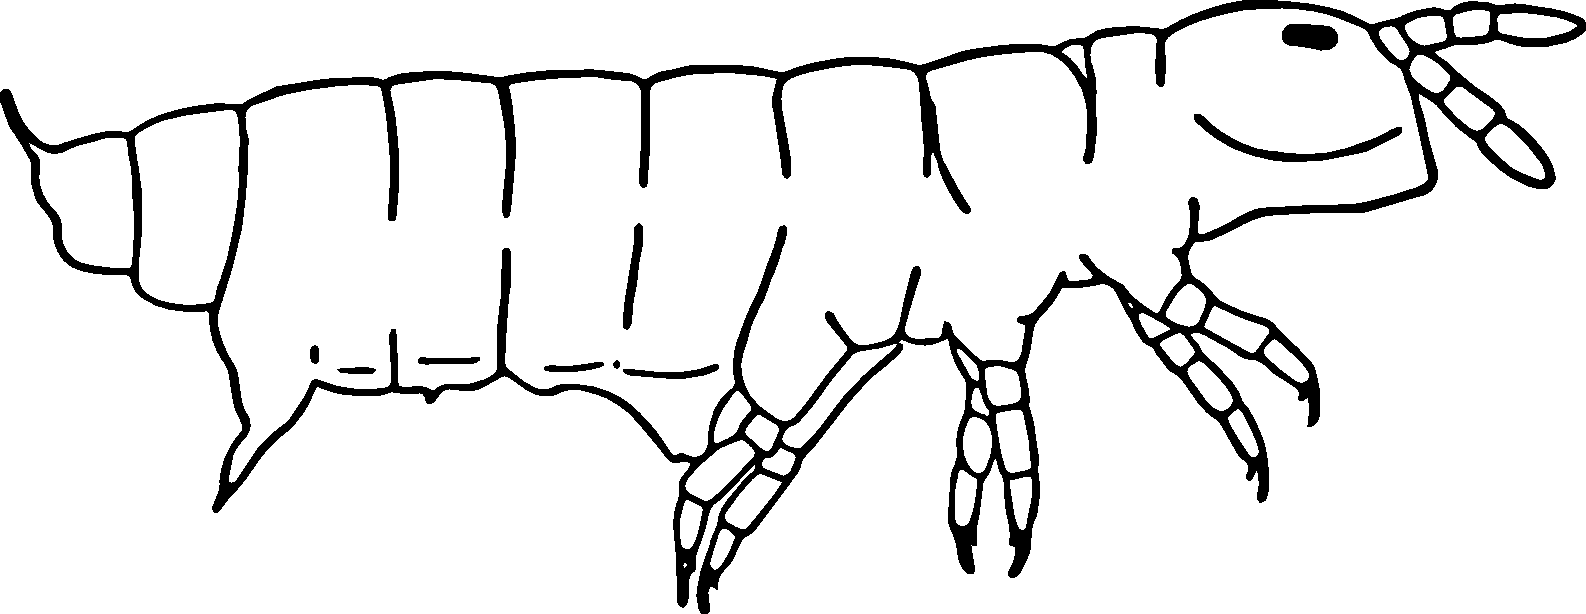
\includegraphics[width=0.4\textwidth]{nonpterygote/hypogastruridHabitus}
  \caption{Poduromorpha (Hypogastruridae) habitus \citep[redrawn from][Fig. 14]{bhlitem30465Insects}}
  \label{fig:hypogasthab}
\end{figure}

\subsubsection{Entomobryomorpha}\index{Entomobryomorpha}
\noindent{}\textit{Diagnostic characters:} Head hypognathous to prognathous, not anteroposteriorly flattened; antennae longer than head; prothorax indistinct dorsally, narrowly articulated with head; abdominal segments 2--4 not fused; body and legs relatively long, thin.\vspace{3mm}

\noindent{}\textit{Natural History:} There are about 8 extant families \citep{SotoAdames501}. Entomobryidae and Tomoceridae are frequently collected in the eastern USA in leaf litter.\vspace{3mm}

\begin{figure}[ht!]
  \centering
    \reflectbox{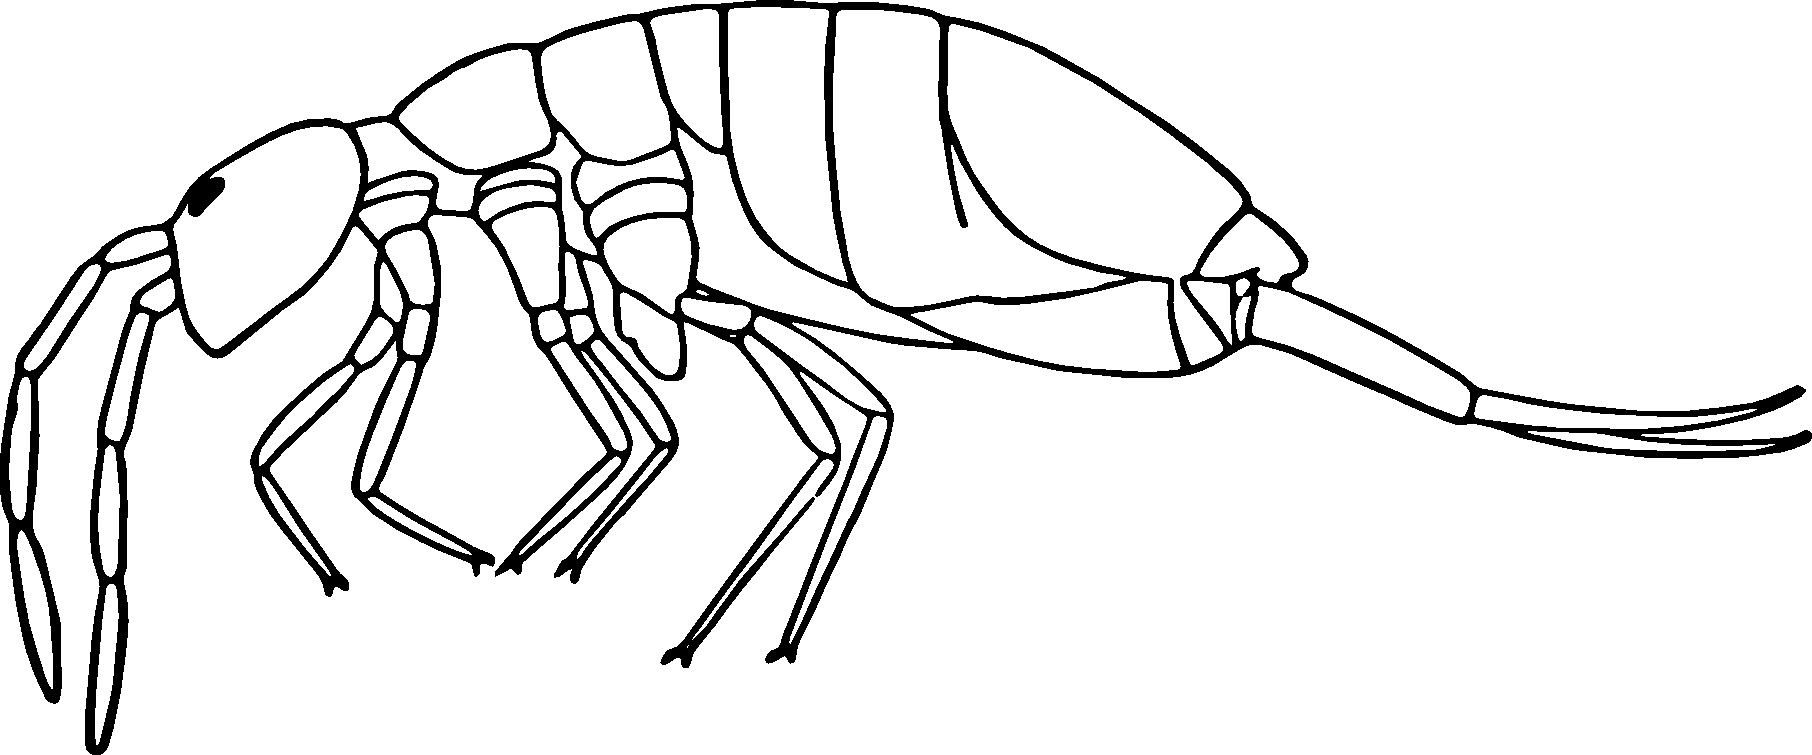
\includegraphics[width=0.5\textwidth]{nonpterygote/entomobryidHabitus.pdf}}
  \caption{Entomobryomorpha (Entomobryidae) habitus \citep[redrawn from][Fig. 17]{bhlitem30465Insects}}
  \label{fig:entomobry}
\end{figure}

\begin{figure}[ht!]
  \centering
    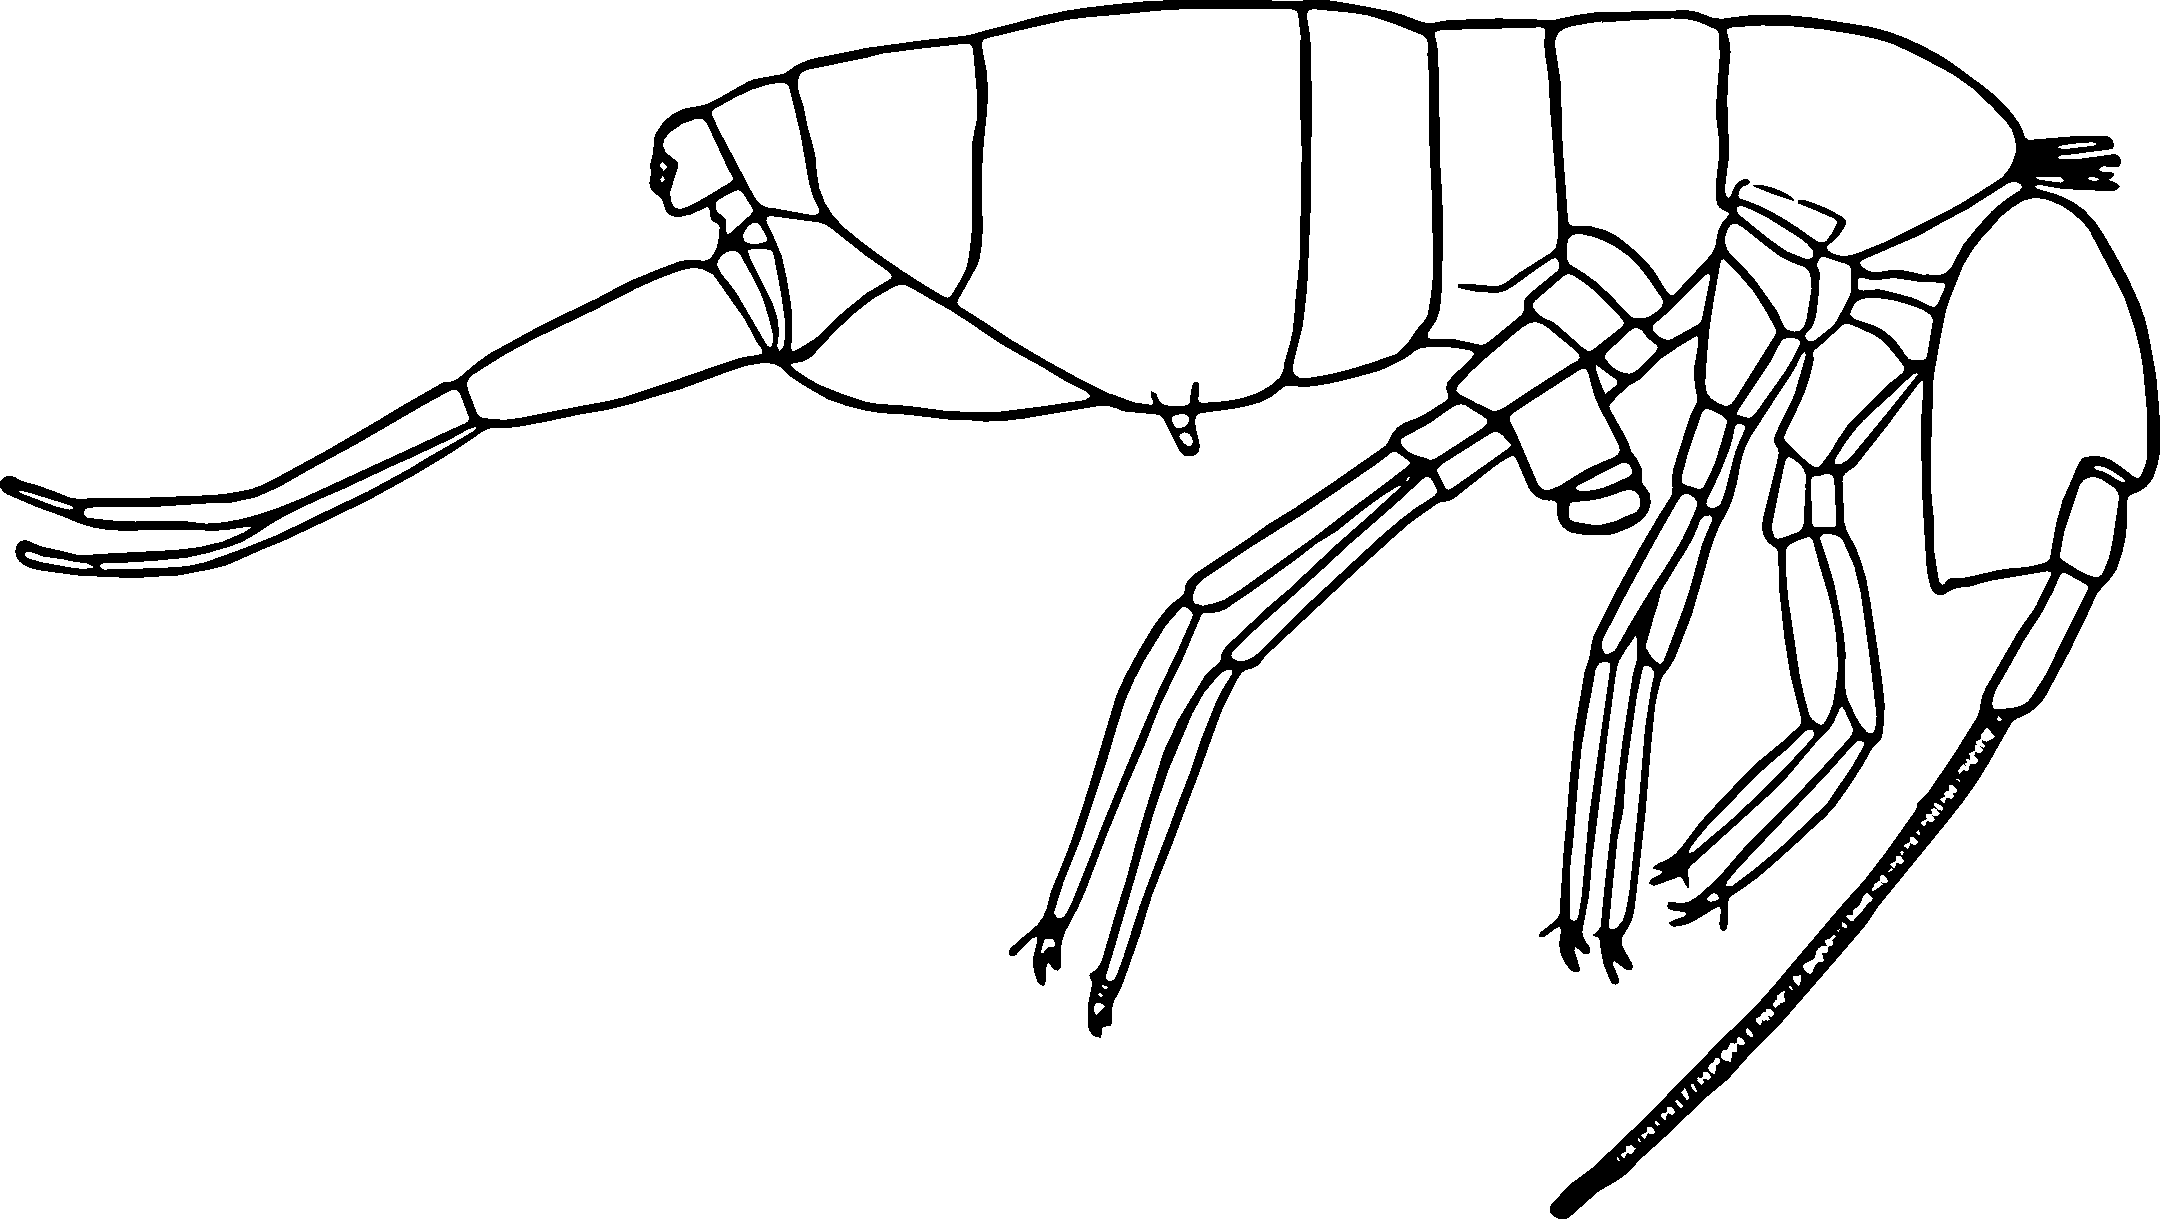
\includegraphics[width=0.45\textwidth]{nonpterygote/tomoceridHabitus}
  \caption{Tomoceridae habitus \citep[redrawn from][Fig. 16]{bhlitem30465Insects}}
  \label{fig:tomocer}
\end{figure}

\section*{Insecta}\index{Insecta}
The remaining arthropods we will examine in lab are true insects. In addition to many internal characters we won't examine (\textit{e.g.}, Johnston's organ) insects can be recognized by:
\begin{itemize}
\item Antennae 3-segmented (\textit{i.e.}, segments with intrinsic musculature), with apical segment (flagellum) usually subdivided
\item Mouthparts not usually enveloped by cuticular evagination (\textit{i.e.}, insects are \textit{ectognathous})
\item Ovipositor present
\end{itemize}

\section{Archaeognatha (Microcoryphia, bristletails)}\index{Archaeognatha}
\noindent{}\textit{Diagnostic characters:} Compound eyes well-developed, adjacent dorsally; maxillary palps longer than legs, subdivided into 7 annuli; labial palps subdivided into 3 annuli; meso- and metacoxa with styli present; styli present on abdominal segments 2--9; abdomen with 3 scaly appendages present apically (2 cerci, 1 terminal appendage); body ``humpbacked'', scaly; paired eversible vesicles usually present on abdominal segments 1--7.\vspace{3mm}

\noindent{}\textit{Natural History:} These insects are frequently found on or around fallen logs and rocks, where they survive on algae, lichens, and decaying matter. There are about 350 known species, in 2 families.\vspace{3mm}

\begin{figure}[ht!]
  \centering
    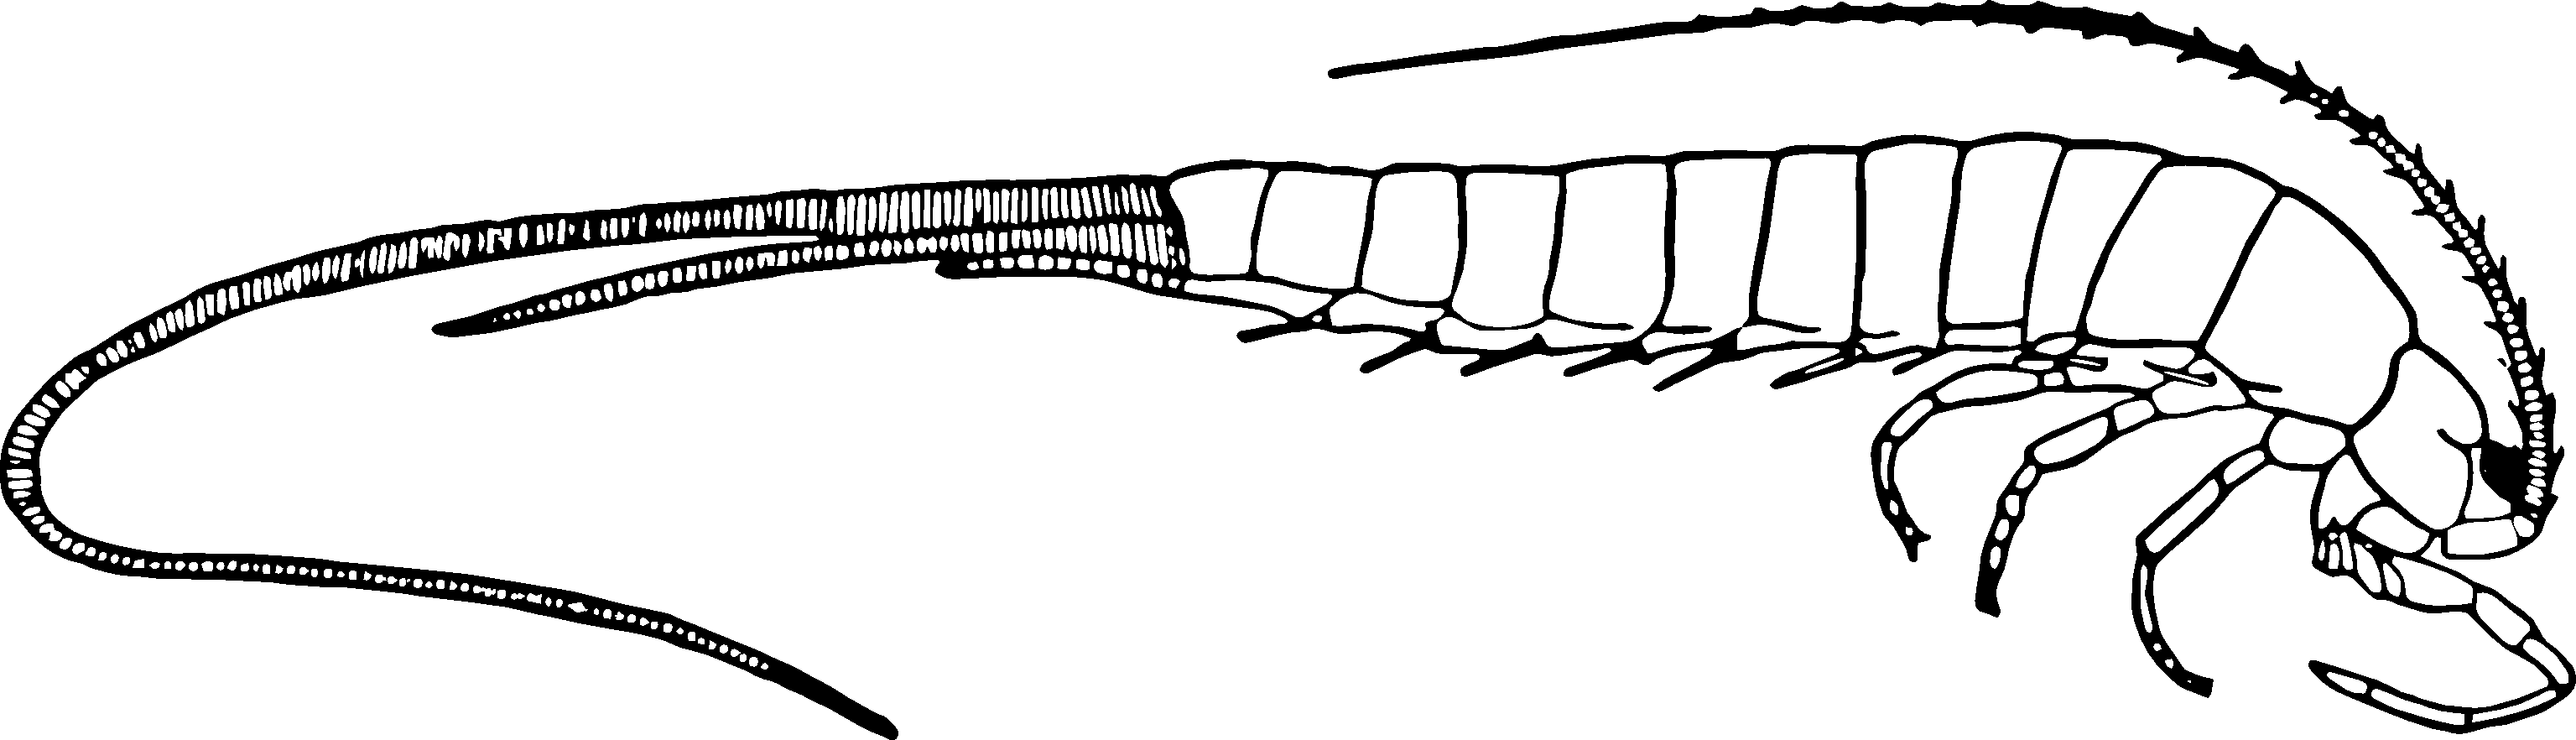
\includegraphics[width=0.7\textwidth]{nonpterygote/archaeognathHabitus}
  \caption{Archaeognathan lateral habitus \cite[redrawn from][Fig. 1]{bhlitem30465Insects}}
  \label{fig:archhabit}
\end{figure}

\begin{figure}[ht!]
  \centering
    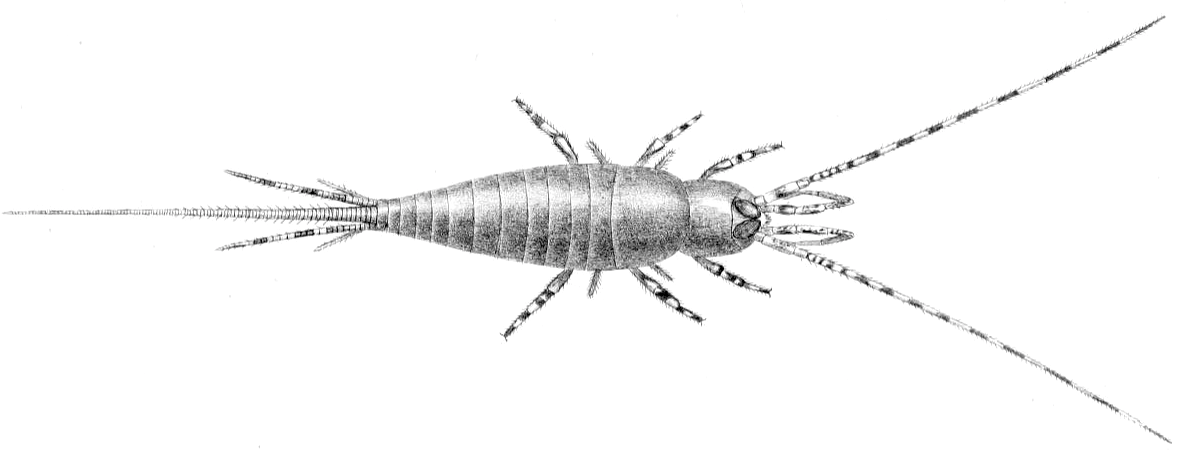
\includegraphics[width=0.8\textwidth]{nonpterygote/archaeoHab2}
  \caption{Archaeognathan dorsal habitus \citep[][Plate 53]{bhlitem43892Lubbock}}
  \label{fig:archhead}
\end{figure}

\begin{theo}
{}Which characteristics would you interpret as ancestral? Can you find evidence that insects are related to other pancrustaceans?\vspace{3mm}

\noindent{}Have you seen these insects move? Why do they have a ``humpbacked'' habitus? Can you find and draw the styli? What might these be remnants of? \end{theo}

\section{Zygentoma (``Thysanura'', in part; silverfish, firebrats)}\index{Zygentoma}

\noindent{}\textit{Diagnostic characters:} Compound eyes small, widely separated; maxillary palps shorter than legs, subdivided into 6 annuli; labial palps subdivided into 4 annuli; styli on meso- and metacoxa absent, usually present on abdominal segments 2--9; abdomen with 3 bare appendages present apically (2 cerci, 1 terminal appendage); body dorsoventrally flattened, scaly; paired eversible vesicles usually present on abdominal segments 1--7.\vspace{3mm}

\noindent{}\textit{Natural History:} Zygentoma is about as diverse as Archaeognatha. Many species inhabit buildings, where they can be pests (eating paper, glue, and other starchy products). Some species live in ant nests, and many can digest cellulose and lignin.\vspace{3mm}

\begin{figure}[ht!]
  \centering
    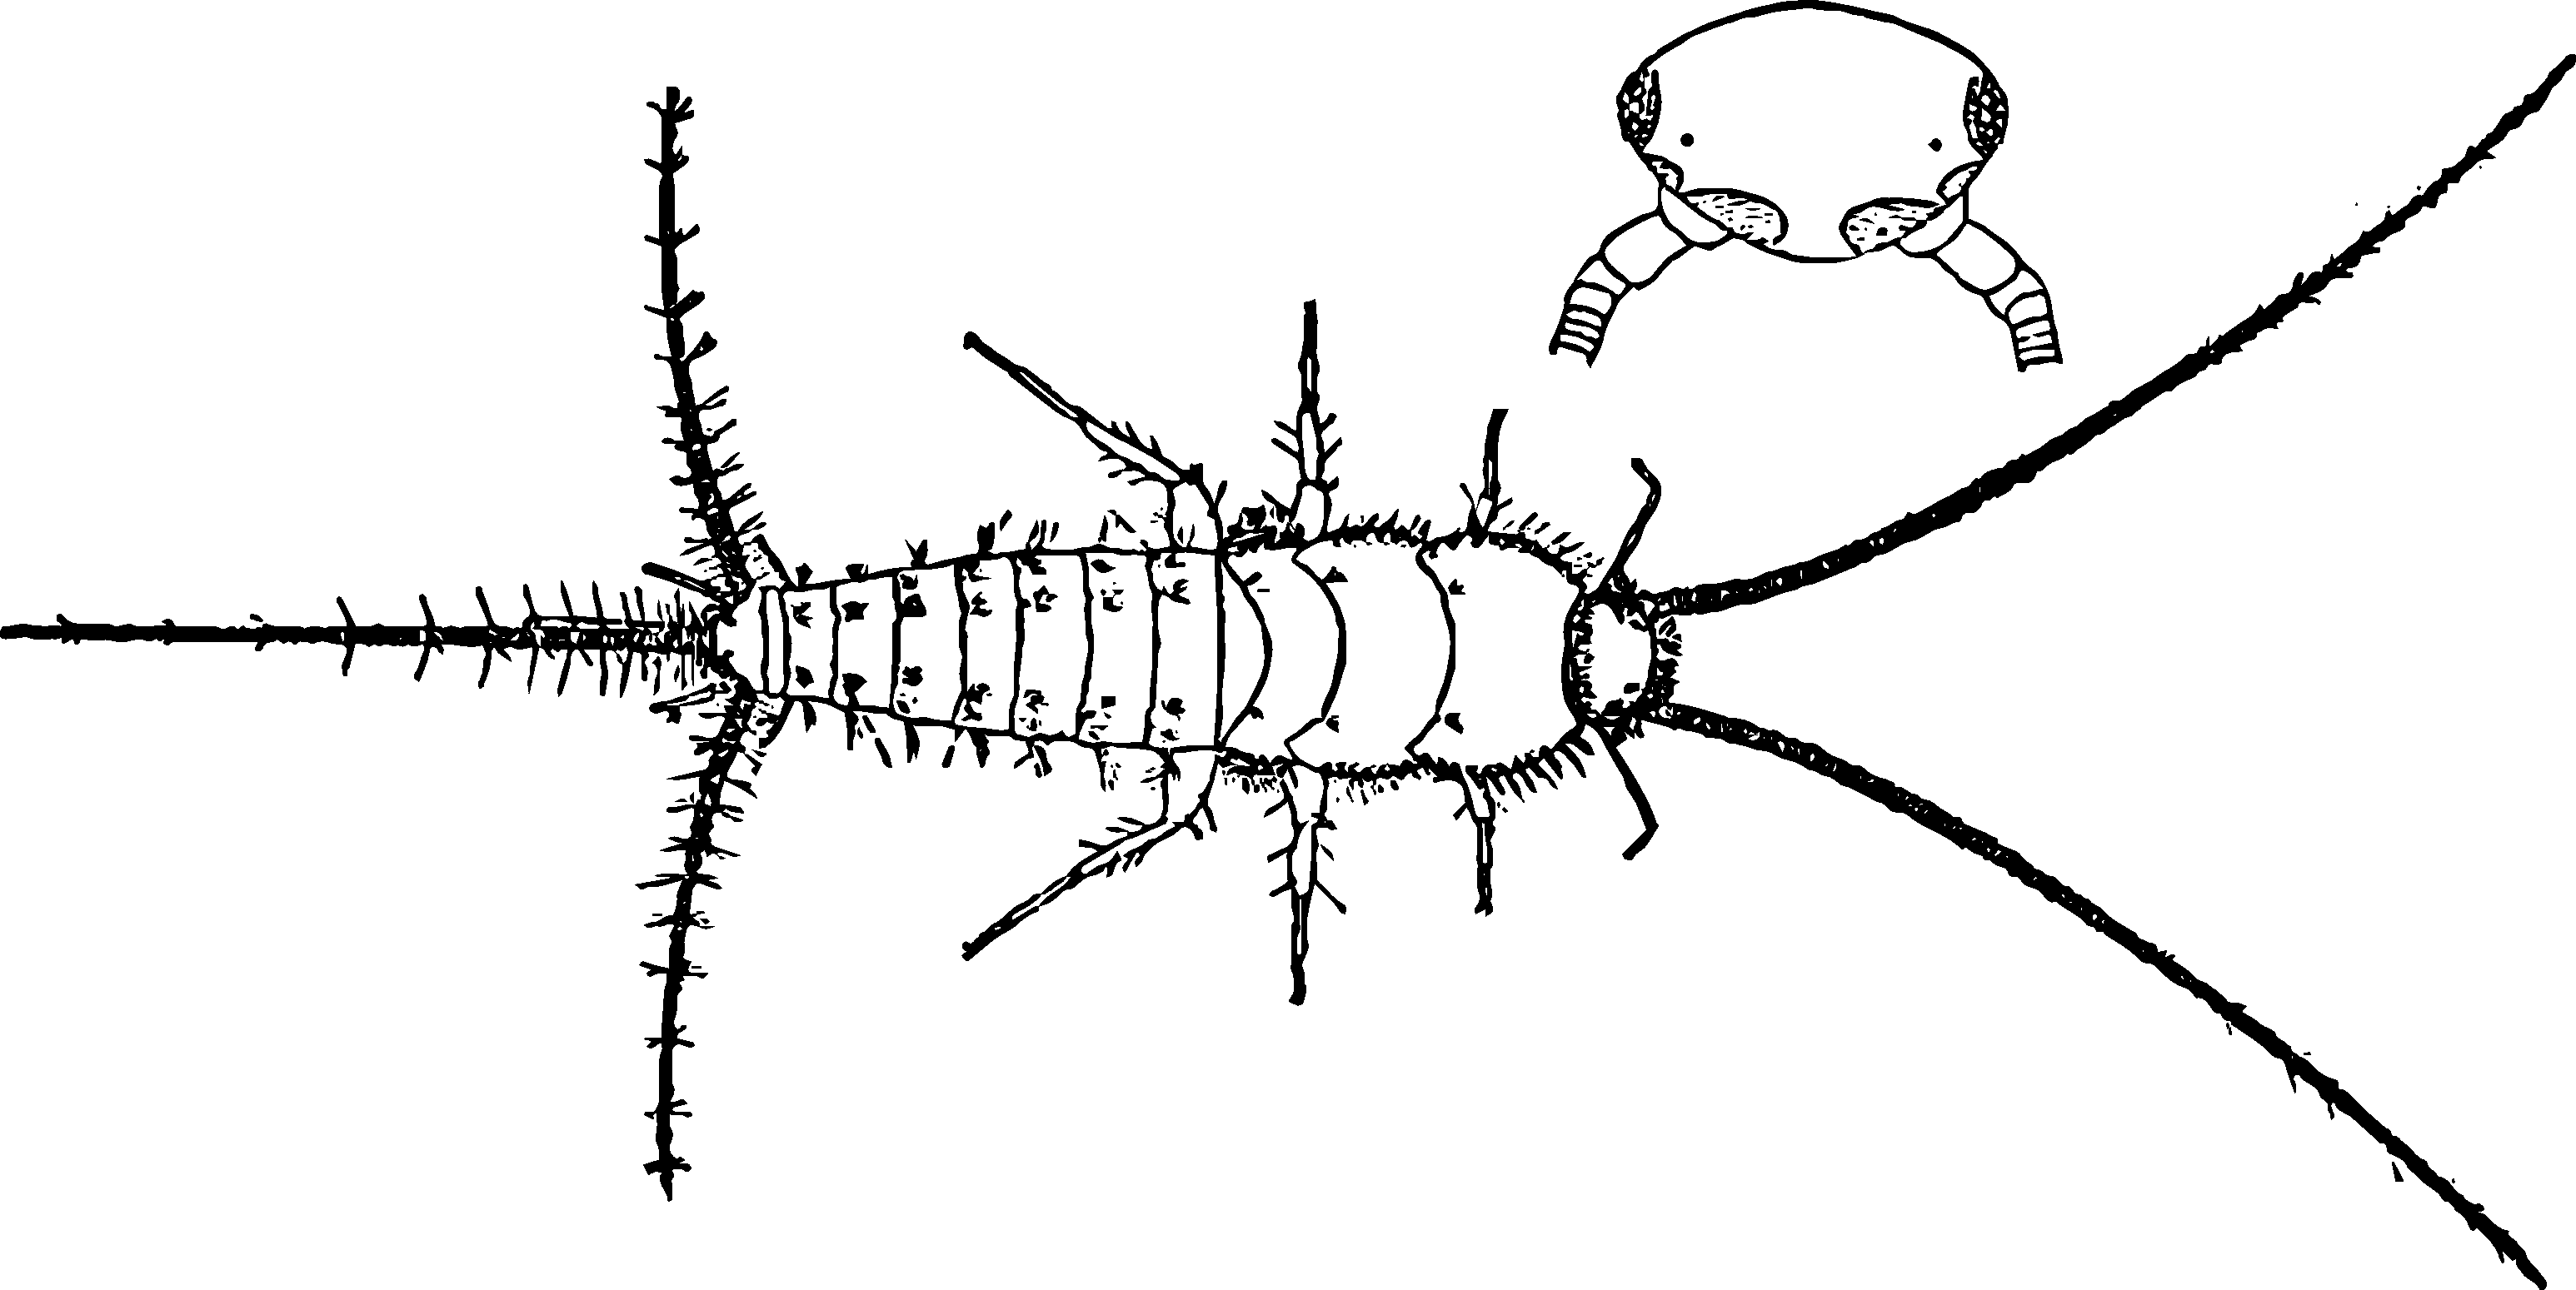
\includegraphics[width=0.8\textwidth]{nonpterygote/lepismatidHabitus}
  \caption{Zygentoma dorsal habitus and head (inset) \citep[redrawn from][Figs. 1, 10]{bhlpart1409lepismat}}
  \label{fig:zygenhabit}
\end{figure}

\begin{figure}[ht!]
  \centering
    \includegraphics[width=0.55\textwidth]{nonpterygote/mandibles.pdf}
  \caption{Mandibles of Symphyla and Apterygota in dorsal view. (A) Myriapoda: Symphyla; (B) Japygidae; (C) Archaeognatha; (D) Collembola; (E) Zygentoma; (F) Protura. Abbreviations: ac=articulating condyle; act=acetabulum; ap=apical process; ar=articulating ridge; at=apical teeth; bs=basal segment; dl=dentate lamella; id=incisor lobe; inl=inner lobe; ma=molar area; mp=molar process; ol=outer lobe \citep[redrawn from][Fig. 1]{bhlpart81512}}
  \label{fig:mandibles}
\end{figure}

\begin{theo}
{}As stated above, Insecta have three traits that set them apart from previous taxa we examined: \textbf{(1)} 3-segmented antenna, with Johnston's organ in the pedicel; \textbf{(2)} exposed mouthparts and a transition to dicondylous mandibles (figures \ref{fig:mandibles}B and F vs. E); \textbf{(3)} presence of ovipositor. Can you describe the adaptive nature of these traits and how they may have contributed to the extraordinary diversity of Insecta?
\end{theo}

\clearpage
\thispagestyle{empty}


\chapter[Paleoptera, Plecoptera, origin of wings]{Paleoptera, Plecoptera,\\ origin of wings}
\section*{Introduction}\index{Pterygota}\index{Pterygota}
In the insect phylogeny and fossil record we observe several adaptive radiations---\textit{i.e.}, events where the emergence of some key innovation or opportunity facilitated the rapid diversification of new forms. The emergence of wings is arguably the most important of these key innovations. The origin of these structures and the selective forces that acted on early versions of wings remain enigmatic. We will discuss hypotheses of the origin of wings before moving on to \textbf{Paleoptera} and the neopteran order \textbf{Plecoptera}.

\section*{Insecta: Pterygota}
We're now looking at insects that have \latinword{wings}, which are usually present as two pairs: fore wings, which articulate with the mesothorax, and hind wings, which articulate with the metathorax.\vspace{3mm}

\begin{theo}
{}Why is the thoracic integument so heavily sclerotized, relative to other body parts and those structures in non-pterygote hexapods? What are the consequences of this phenotype?
\end{theo}

\section*{Pterygota: Paleoptera}
In the next two orders, the wing base inhibits wing folding---\textit{i.e.}, the wings are held out or vertically over the thorax when at rest. The latest evidence indicates that these two orders comprise a monophyletic group, called Paleoptera.

\section{Ephemeroptera (mayflies)}\index{Ephemeroptera}%Ephemeridae in Penns Creek; add Caenidae or Leptohyphidae for operculate gills (protection in turbid water)

\subsection{Naiads}
Mayflies are aquatic in their immature stages, which are usually referred to as naiads or larvae (Not to be confused with the immature stages of holometabolous insects; more on that later.) Mayflies spend the vast majority of their lives as naiads, and we can see numerous adaptations for feeding and locomotion in this stage. Examine naiads of the following families, which should give you a sense of the phenotypic variation in Ephemeroptera: \textbf{Baetidae}, \textbf{Heptageniidae}, and \textbf{Ephemeridae}.\\\index{Baetidae}\index{Heptageniidae}\index{Ephemeridae}

\begin{figure}[ht!]
    \centering
    \begin{subfigure}[ht!]{0.6\textwidth}
        \includegraphics[width=\textwidth]{paleoptera/ephemNaiad}
        \caption{}
        \label{fig:ephemeridlarva}
    \end{subfigure}
    \hfill
    \begin{subfigure}[ht!]{0.25\textwidth}
        \includegraphics[width=\textwidth]{paleoptera/ephemNaiadHead}
        \caption{}
        \label{fig:ephemeridlarvahead}
    \end{subfigure}
    \caption{Ephemeridae naiad \textbf{(a)} habitus \citep[modified from][Fig. 59]{bhlpart97188ephem}; \textbf{(b)} head \citep[redrawn from][Fig. 50]{bhlpart97188ephem}}
    \label{fig:ephemeridLarvae}
\end{figure}

\begin{theo}
{}The bodies and head shapes of these mayflies yield clues about their life histories. Can you predict where each family is typically found and how eat it eats and moves through the water?\vspace{3mm}

\noindent{}Can you find evidence of developing wings? Describe your observations.
\end{theo}

\begin{figure}[ht!]
  \centering
    \reflectbox{\includegraphics[width=0.7\textwidth]{paleoptera/baetidNaiad}}
  \caption{Baetidae naiad \citep[modified from][Fig. 240]{bhlpart97188ephem}}
  \label{fig:baetidNaiad}
\end{figure}

\begin{figure}[ht!]
  \centering
    \includegraphics[width=0.6\textwidth]{paleoptera/heptageniidNaiad}
  \caption{Heptageniidae naiad \citep[modified from][Fig. 360]{bhlpart97188ephem}}
  \label{fig:heptageniidNaiad}
\end{figure}
\FloatBarrier

\subsection{Adults}
\noindent{}Wing venation and appendage traits offer important characters for family-level diagnosis of adults. See if you can understand the traits listed below characters, which could be used to recognize adults of three common families in the northeastern US: \textbf{Ephemeridae}, \textbf{Heptageniidae}, and \textbf{Baetidae}. Note that there are many other common mayfly families in this part of the world!%add diagnostic traits for adults at the order level!!!

\subsubsection{Ephemeridae (burrower mayflies, drakes)}\index{Ephemeridae}
\noindent{}\textit{Diagnostic characters:} Male compound eye round, unmodified; cubital intercalaries (between CuA and CuP) in fore wing not present as 2 parallel pairs; \texorpdfstring{MP\textsubscript{2}}{ }{ }of fore wing sharply angled towards Cu proximally; hind wing large, visible, with many veins; hind leg tarsus with 3-4 tarsomeres; apex of abdomen with 2--3 long appendages.\vspace{3mm}

\noindent{}\textit{Natural history:} Naiads have fossorial legs, which they use to burrow in substrate. They scavenge or predate on other arthropods. There are approximately 150 described spp. worldwide.\vspace{3mm}

\begin{figure}[ht!]
    \centering
       \includegraphics[width=0.8\textwidth]{paleoptera/Ephemeridae}
    \caption{Ephemeridae. \citep[modified from][Plate LXXV]{bhlitem81095ephem}}\label{fig:ephemerid}
\end{figure}

\subsubsection{Baetidae (minnow mayflies)}\index{Baetidae}
\noindent{}\textit{Diagnostic characters:} Adult small, usually \textless10 mm long; male compound eye turbinate (figure \ref{fig:baetid2}); cubital intercalaries (between CuA and CuP) in fore wing not present as 2 parallel pairs; \texorpdfstring{MP\textsubscript{2}}{ }{ }of fore wing not sharply angled towards Cu proximally; hind wing small or absent; hind leg tarsus with 4 tarsomeres; apex of abdomen with 2 long appendages.\vspace{3mm}

\noindent{}\textit{Natural history:} Naiads have streamlined shape, adapted for swimming in the water. They feed primarily on algae. There are approximately 1,000 described spp. worldwide.\vspace{3mm}

\begin{figure}[ht!]
    \centering
    \begin{subfigure}[ht!]{0.42\textwidth}
        \includegraphics[width=\textwidth]{paleoptera/BaetidaeFemHabitus}
        \caption{}
        \label{fig:baetid1}
    \end{subfigure}
    \hfill
    \begin{subfigure}[ht!]{0.45\textwidth}
        \includegraphics[width=\textwidth]{paleoptera/BaetidaeMaleHabitus}
        \caption{}
        \label{fig:baetid2}
    \end{subfigure}
    \caption{Baetidae. \textbf{(a)} Female habitus, photo (CC BY 2.0) by Andrey Zharkikh \url{https://flic.kr/p/AnyRSm}; \textbf{(b)} Male habitus, not conspecific with \ref{fig:baetid1}, photo (CC BY-SA 2.0) by Bernard DuPont \url{https://flic.kr/p/Ru6AuY}}\label{fig:baetids}
\end{figure}

\subsubsection{Heptageniidae (flat-headed mayflies, stream mayflies)}\index{Heptageniidae}
\noindent{}\textit{Diagnostic characters:} Adult size variable; male compound eye round, unmodified; cubital intercalaries (between CuA and CuP) in fore wing present as 2 parallel pairs; \texorpdfstring{MP\textsubscript{2}}{ }{ }of fore wing not sharply angled towards Cu proximally; hind wing large, visible, with many veins; hind leg tarsus with 5 tarsomeres; apex of abdomen with 2 long appendages.\vspace{3mm}

\noindent{}\textit{Natural history:} Naiads have flattened shape, adapted for living in the boundary layer in lotic systems. They have diverse feeding habits, with many species scraping algae, while others scavenge or predate on other invertebrates. There are approximately 500 described spp. worldwide.\vspace{3mm}

\begin{figure}[ht!]
    \centering
    \begin{subfigure}[ht!]{0.5\textwidth}
        \includegraphics[width=\textwidth]{paleoptera/HeptageniidHabitus}
        \caption{}
        \label{fig:heptageniid1}
    \end{subfigure}
    \hfill
    \begin{subfigure}[ht!]{0.4\textwidth}
        \includegraphics[width=\textwidth]{paleoptera/HeptageniidWing}
        \caption{}
        \label{fig:heptageniid2}
    \end{subfigure}
    \caption{Heptageniidae. \textbf{(a)} Habitus, drawn from photo (CC BY-SA) by Richard Bartz \url{https://commons.wikimedia.org/wiki/File:Ephemeroptera_2.jpg}; \textbf{(b)} fore wing venation \citep[redrawn from][Fig. 61]{comstock1918wings}}\label{fig:heptageniid}
\end{figure}

\FloatBarrier

\section{Odonata (dragonflies, damselflies)}\index{Odonata}
Like their putative sister lineage, Ephemeroptera, immature Odonata are almost exclusively aquatic. All species are predaceous in all stages, with adaptations that facilitate prey tracking, stalking, and capture.\vspace{3mm}%add naiads and adults diag chars?

\begin{theo}
{}Can you list at least three adaptations you see across Odonata families that you hypothesize facilitate predation?\\

\noindent{}Odonata adults are prepared using an unorthodox approach, relative to other Pterygota (see Section \ref{odeprep}). Why?\index[preps]{Odonata}
\end{theo}\vspace{3mm}

\noindent{}Another conspicuous synapomorphy for Odonata is the evolution of a secondary copulatory organ ventrally on the first abdominal segment of males. Females are grabbed and held behind the head by the male, using his apical abdominal appendages. Be sure to look for adaptations associated with this unusual copulatory habit.\vspace{3mm}

\begin{theo}
{}Sketch a feature on the female head that you suspect is an adaptation for this kind of copulation. How do you think the secondary male genitalia evolved? What did the early, intermediate form look like?
\end{theo}\vspace{3mm}

\noindent{}Odonata is the first group where each wing has a distinct pterostigma (pigmented spot on anterior edge of wing). The pterostigma is not only highly pigmented but also more sclerotized and more massive than other wing areas.\vspace{3mm}

\subsection{Anisoptera (dragonflies)}

\subsubsection{Gomphidae (clubtails)}\index{Gomphidae}
\noindent{}\textit{Diagnostic characters:} Compound eyes separated dorsally, triangular wing cells (``triangles'') in fore wing and hind wing similar in shape and location, apical abdominal segments often expanded laterally, forming a ``club''.\vspace{3mm}

\noindent{}\textit{Natural history:} Larvae are usually found in lotic systems, where they bury themselves in the substrate and wait for prey. Look for adults on flat perches, \textit{e.g.}, on the ground or on leaves. Approximately 900 spp. have been described worldwide.\vspace{3mm}

\begin{figure}[ht!]
    \centering
    \begin{subfigure}[ht!]{0.4\textwidth}
        \includegraphics[width=\textwidth]{paleoptera/GomphidaeWing}
        \caption{}
        \label{fig:gomphid1}
    \end{subfigure}
    \hfill
    \begin{subfigure}[ht!]{0.55\textwidth}
        \reflectbox{
        \includegraphics[width=\textwidth]{paleoptera/gomphidBody}}
        \caption{}
        \label{fig:gomphid2}
    \end{subfigure}
    \caption{Gomphidae. \textbf{(a)} Wing venation \citep[][Fig. 229]{comstock1918wings}; \textbf{(b)} head (twisted 90\textdegree), thorax, and abdomen \citep[redrawn from][Fig. 4:17 f1]{bhlitem126080aquatic}}\label{fig:gomphids} 
\end{figure}

\subsubsection{Aeshnidae (darners, hawkers)}\index{Aeshnidae}
\noindent{}\textit{Diagnostic characters:} Compound eyes adjacent dorsally, triangular wing areas (``triangles'') in fore wing and hind wing similar in shape and location, ovipositor well developed.\vspace{3mm}

\noindent{}\textit{Natural history:} Larvae are often thought of as being part of the ``climber'' guild of aquatic insects, as they are usually found in aquatic vegetation. Do they appear to be adapted for climbing and hunting in vegetation (see figure \ref{fig:OdonataLarva})? Adults are typically large and are very strong fliers. One can find these dragonflies in/near almost any aquatic habitat. Approximately 440 spp. have been described worldwide.\vspace{3mm}

\begin{figure}[ht!]
    \centering
    \begin{subfigure}[ht!]{0.48\textwidth}
        \includegraphics[width=\textwidth]{paleoptera/AeshnidWings}
        \caption{}
        \label{fig:aeshnid1}
    \end{subfigure}
    \hfill
    \begin{subfigure}[ht!]{0.3\textwidth}
        \includegraphics[width=\textwidth]{paleoptera/aeshnidHead}
        \caption{}
        \label{fig:aeshnid2}
    \end{subfigure}
    \caption{Aeshnidae. \textbf{(a)} Wing venation \citep[][Fig. 236]{comstock1918wings}; \textbf{(b)} head in dorsal view \citep[][Plate 22, Fig. 3]{aeshnaNorthAmerica}}\label{fig:aeshnids}
\end{figure}

\begin{figure}[ht!]
  \centering
    \reflectbox{%
    \includegraphics[width=0.7\textwidth]{paleoptera/aeshnidHabitus}}
  \caption{Aeshnidae lateral habitus \citep[][Plate 28, Fig. 5]{aeshnaNorthAmerica}}
  \label{fig:aeshnidHabitus}
\end{figure}

\subsubsection{Libellulidae (common skimmers)} \index{Libellulidae}
\noindent{}\textit{Diagnostic characters:} Compound eyes meeting dorsally, triangles in fore wing and hind wing different in shape, hind wing with boot-shaped area, ovipositor absent.\vspace{3mm}

\noindent{}\textit{Natural history:} Larvae are usually thought of as ``sprawlers'', which generally sit relatively still on the bottom, in the sediment, waiting for prey. Can you see major morphological differences between these larvae and other odonates? Adults are diverse in size, color, and habitat. More than 1,000 spp. have been described worldwide.\vspace{3mm}

\begin{figure}[ht!]
    \centering
    \begin{subfigure}[ht!]{0.5\textwidth}
        \includegraphics[width=\textwidth]{paleoptera/LibellulidWings}
        \caption{}
        \label{fig:libelwing}
    \end{subfigure}
    \hfill
    \begin{subfigure}[ht!]{0.25\textwidth}
        \includegraphics[width=\textwidth]{paleoptera/LibellulidaeHead}
        \caption{}
        \label{fig:libelbody}
    \end{subfigure}
    \caption{Libellulidae. \textbf{(a)} Wing venation \citep[][Fig. 240]{comstock1918wings}; \textbf{(b)} head (illustration by Laura Porturas, Penn State)}\label{fig:libell}
\end{figure}

\subsection{Zygoptera (damselflies)}
\subsubsection{Calopterygidae (jewelwings, broad-winged damselflies)}\index{Calopterygidae}
\noindent{}\textit{Diagnostic characters:} Wings tapered at base, numerous antenodal crossveins present (proximal to nodus).\vspace{3mm}

\noindent{}\textit{Natural history:} Like other damselflies, larvae are usually thought of as climbers. Larvae and adults are usually found along streams (\textit{i.e.}, lotic systems). Approximately 150 spp. have been described worldwide.\vspace{3mm}

\begin{figure}[ht!]
    \centering
    \begin{subfigure}[ht!]{0.45\textwidth}
        \includegraphics[width=\textwidth]{paleoptera/CalopterygidWing}
        \caption{}
        \label{fig:calopwing}
    \end{subfigure}
    \hfill
    \begin{subfigure}[ht!]{0.45\textwidth}
        \includegraphics[width=\textwidth]{paleoptera/CalopterygidHabitus}
        \caption{}
        \label{fig:calopbody}
    \end{subfigure}
    \caption{Calopterygidae. \textbf{(a)} Wing venation \citep[][Fig. 235]{comstock1918wings}; \textbf{(b)} habitus \citep[redrawn from][Plate XLVIII, Fig. 2]{bhlitem82229}}\label{fig:calop}
\end{figure}

\subsubsection{Coenagrionidae (bluets, narrow-winged damselflies)}\index{Coenagrionidae}
\noindent{}\textit{Diagnostic characters:} wings stalked at base, few antenodal crossveins present, \texorpdfstring{M\textsubscript{3}}{ }{ } arises near nodus, quadrangle wing cell actually triangular.\vspace{3mm}

\noindent{}\textit{Natural history:} Given the high level of diversity (\textgreater1,100 spp.), one can find these odonates in almost any aquatic habitat. Like other damselflies, larvae are usually thought of as climbers. Females oviposit in or near vegetation.\vspace{3mm}

\begin{figure}[ht!]
    \centering
    \begin{subfigure}[ht!]{0.45\textwidth}
        \includegraphics[width=\textwidth]{paleoptera/CoenagrionidWing}
        \caption{}
        \label{fig:coenwing}
    \end{subfigure}
    \hfill
    \begin{subfigure}[ht!]{0.5\textwidth}
        \reflectbox{%
          \includegraphics[width=\textwidth]{paleoptera/coenagBody}}
        \caption{}
        \label{fig:coenbody}
    \end{subfigure}
    \caption{Coenagrionidae. \textbf{(a)} Fore wing; \textbf{(b)} habitus \citep[redrawn from][Fig. 4:71a]{bhlitem126080aquatic}}\label{fig:coenag}
\end{figure}

\subsubsection{Lestidae (spreadwings)}\index{Lestidae}
\noindent{}\textit{Diagnostic characters:} wings stalked at base, few antenodal crossveins present, \texorpdfstring{M\textsubscript{3}}{ }{ } arises near arculus, quadrangle wing cell actually quadrangular.\vspace{3mm}

\noindent{}\textit{Natural history:} Naiads are found in a variety of aquatic environments and have a distinctive, elongate habitus and a spoon-like labium. Unlike other damselflies, adult lestids usually rest on vegetation with their wings at least partially spread. Approximately 150 spp. have been described worldwide.\vspace{3mm} 

\begin{figure}[ht!]
    \centering
    \begin{subfigure}[ht!]{0.45\textwidth}
        \includegraphics[width=\textwidth]{paleoptera/LestidWing}
        \caption{}
        \label{fig:lestwing}
    \end{subfigure}
    \hfill
    \begin{subfigure}[ht!]{0.45\textwidth}
        \reflectbox{%
          \includegraphics[width=\textwidth]{paleoptera/LestidHabitus}}
        \caption{}
        \label{fig:lestbody}
    \end{subfigure}
    \caption{Lestidae. \textbf{(a)} Wing venation \citep[][Fig. 232]{comstock1918wings}; \textbf{(b)} habitus (illustration by Laura Porturas, Penn State)}\label{fig:lestid}
\end{figure}%https://www.biodiversitylibrary.org/page/40665889

\subsection{Naiads}
Take a moment to observe Odonata naiads of these families under your microscope. Could you determine each family by sight? Can you see the different predatory tactics of the different families?\vspace{3mm}

\begin{theo}
{}Can you find and describe two naiadal adaptations for predation?\vspace{3mm}

\noindent{}What morphological differences to you see between a dragonfly naiad and a damselfly naiad? Make a sketch.
\end{theo}

\begin{figure}[ht!]
    \centering
    \begin{subfigure}[ht!]{0.45\textwidth}
        \includegraphics[width=\textwidth]{paleoptera/aeshnidLarva}
        \caption{}
        \label{fig:OdonataLarva}
    \end{subfigure}
    \hfill
    \begin{subfigure}[ht!]{0.47\textwidth}
       \includegraphics[width=\textwidth]{paleoptera/odonataLarva}
        \caption{}
        \label{fig:OdonataLarvaLabium}
    \end{subfigure}
    \caption{Odonata naiads. \textbf{(a)} Aeshnidae naiad \citep[][Fig. 59]{bhl128276}; \textbf{(b)} libellulid labium, retracted and expanded \citep[redrawn from][Fig. 1]{bhlpart204280odelarva}}\label{fig:odeLarvae}
\end{figure}

\FloatBarrier

\section*{Pterygota: Neoptera}\index{Neoptera}
The remaining insect orders are classified in Neoptera, a lineage whose members can pull their wings over their abdomens when they're at rest. This movement is accomplished by flexing a pleural muscle that inserts on the 3rd axillary sclerite. The wing then folds along flexion lines that are not present in Paleoptera, allowing the wing to be pulled back posteriorly.\vspace{3mm}

\begin{theo}
{}In this unit we've touched on two evolutionary events that are considered to be \latinword{key innovations}: the origin of wings and the the origin of neoptery. Why do you think these two adaptations led to explosive diversification?
\end{theo}

\section{Plecoptera (stoneflies)}\index{Plecoptera}%add Pteronarcyidae (giant stoneflies) and Peltoperlidae (roach-like) need to sight ID?! why not ID the order and describe whether it has gill tufts and nota shape, glossa length, etc.
Like the previous two orders, Plecoptera are aquatic during their immature stages and semi-aquatic/terrestrial as adults. More than 100 million years of evolution separates Plecoptera from Paleoptera \citep{Misof763}, however, so stoneflies are not closely related (relatively speaking) to dragonflies and mayflies. It is useful to treat them here, however, as they have similar habits to mayflies, are important for monitoring water quality (like Ephemeroptera), and have inspired much speculation on the origin of wings.

\subsection*{Naiads}
Stonefly naiads are almost exclusively found in lotic environments---\textit{e.g.}, clear, clean, highly oxygenated streams---and they are generally very sensitive to water quality. The immature stages develop as predators of other aquatic invertebrates or as shredders of vegetative material. They can be recognized from other aquatic non-holometabolous insects by (a) the presence of two tarsal claws on each leg and (b) two cerci on the apex of the abdomen.\vspace{3mm}

\noindent{}Select specimens of at least three families and look for phenotypic differences in these diagnostic traits:
\begin{itemize}
\item presence/absence of gill tufts on the thorax and/or abdomen
\item width and shape of nota in dorsal view
\end{itemize}

\subsection*{Adults}
Stoneflies are generally not good dispersers and so are found near the features from which their naiads emerged. The diagnostic features can be subtle, so it's important to spend some time understanding the relevant morphology:

\begin{itemize}
\item Glossa length relative to paraglossa length (\textit{cf}.\footnote{From the Latin verb \textit{conferre}, to bring together, used here to invite the reader to compare the listed taxa.} Perlidae or Perlodidae \textit{vs}. Leuctridae or Capniidae)
\item Presence/location of gill remnants (\textit{cf}. Perlidae \textit{vs}. Perlodidae. Hint: look near the coxae)
\item Wing phenotype at rest (\textit{cf}. Perlidae or Perlodidae \textit{vs}. Leuctridae)
\item Wing venation (figure \ref{fig:plecowings})
\item Relative length of the cerci (\textit{cf}. Perlidae or Perlodidae \textit{vs}. Leuctridae)
\end{itemize}

\begin{figure}[ht!]
  \centering
    \includegraphics[width=0.65\textwidth]{paleoptera/PlecopteraWings}
  \caption{Plecoptera wing venation \citep[modified from][Fig. 1]{bhl29875}. Caption, from the source and edited slightly: ``C = Costa; Sc = Subcosta; R = Radius; M = Media; Cu = Cubitus; A = Anal; Rs = radial sector, the principal branch of the Radius. A plus sign between letters indicates these veins are fused together. The more typical crossveins are designated as follows: h = humeral; r = inter-radial; r-m = radio-median; m = median; m-cu = medio-cubital crossvein; cu-a = cubito-anal. Other veins and areas are designated as follows: arc = arculus, which is a crossvein to which is often added a deflected basal portion of either of the veins it connects; st = stigma, a thickening in the costal space beyond the tip of the sub-costal vein; a = anal cell; int = inter-radial cell; CORD = the cord, a line of transverse joinings, composed of crossveins and the bases of principal forks, extending from the stigma obliquely backward to the cubital vein. The broad area bounded externally by the cord is sometimes spoken of as the wing disc.''}
  \label{fig:plecowings}
\end{figure}

\subsection{Arctoperlaria}
\subsubsection{Perlidae (common stoneflies)}\index{Perlidae}
\noindent{}\textit{Diagnostic characters:} Glossae much shorter than paraglossae; cercus longer than pronotum width; branched gill remnants present behind leg bases; hind wing with 5 or fewer anal veins; fore wing not rolled around body.\vspace{3mm}

\noindent{}\textit{Natural history:} More than 80 species are known, the vast majority of which can be found in eastern North America. Naiads are predators of other invertebrates.\vspace{3mm} 

\begin{figure}[ht!]
    \centering
    \begin{subfigure}[ht!]{0.45\textwidth}
        \includegraphics[width=\textwidth]{paleoptera/PerlidWings}
        \caption{}
        \label{fig:perlid1}
    \end{subfigure}
    \qquad
    \begin{subfigure}[ht!]{0.45\textwidth}
        \includegraphics[width=\textwidth]{paleoptera/perlid}
        \caption{}
        \label{fig:perlid2}
    \end{subfigure}
    \caption{Perlidae. \textbf{(a)} Wings \citep[modified from][Plate 11, Fig. 3]{bhl29875}; \textbf{(b)} dorsal habitus \citep[redrawn from][Fig. 18]{bhl29875}}\label{fig:perlids}
\end{figure}

\subsubsection{Perlodidae}\index{Perlodidae}
\noindent{}\textit{Diagnostic characters:} Glossae much shorter than paraglossae; cercus longer than pronotum width; branched gill remnants absent; cubito-anal crossvein arising distal to anal cell; 4 or more Cu crossveins on fore wing, 2A forked; hind wing with 5--10 anal veins; fore wing not rolled around body.\vspace{3mm}

\noindent{}\textit{Natural history:} More than 100 species are known. Naiads are somewhat flattened dorso-ventrally and are predators of other invertebrates.\vspace{3mm}

\begin{figure}[ht!]
    \centering
    \begin{subfigure}[ht!]{0.4\textwidth}
        \includegraphics[width=\textwidth]{paleoptera/PerlodidWings}
        \caption{}
        \label{fig:perlodid1}
    \end{subfigure}
    \qquad
    \begin{subfigure}[ht!]{0.5\textwidth}
        \includegraphics[width=\textwidth]{paleoptera/PerlodidHabitus}
        \caption{}
        \label{fig:perlodid2}
    \end{subfigure}
    \caption{Perlodidae. \textbf{(a)} Wings \citep[modified from][Plate 9, Fig. 1]{bhl29875}; \textbf{(b)} dorsal habitus \citep[modified from][Fig. 12]{bhl29875}}\label{fig:perlodids}
\end{figure}

\subsubsection{Leuctridae (rolled-wing stoneflies)}\index{Leuctridae}
\noindent{}\textit{Diagnostic characters:} Glossae same length as paraglossae; cercus very short composed of one segment; branched gill remnants absent; cubito-anal crossvein arising distal to or from anal cell; 4 or more Cu crossveins on fore wing; 2A forked; fore wings rolled around body.\vspace{3mm}

\noindent{}\textit{Natural history:} Relatively small as adults ($\sim$1 cm long). Naiads feed on plants. More than 350 species are known worldwide, distributed primarily across the Holarctic.\vspace{3mm}

\begin{figure}[ht!]
    \centering
    \begin{subfigure}[ht!]{0.4\textwidth}
        \includegraphics[width=\textwidth]{paleoptera/LeuctridWings}
        \caption{}
        \label{fig:leuctrid1}
    \end{subfigure}
    \qquad
    \begin{subfigure}[ht!]{0.5\textwidth}
        \includegraphics[width=\textwidth]{paleoptera/LeuctridHabitus}
        \caption{}
        \label{fig:leuctrid2}
    \end{subfigure}
    \caption{Leuctridae. \textbf{(a)} Wings \citep[redrawn from][Plate 32, Fig. 1]{bhl29875}; \textbf{(b)} dorsal habitus \citep[modified from][Fig. 26]{bhl29875}}\label{fig:leuctrids}
\end{figure}

\subsubsection{Capniidae (winter stoneflies)}\index{Capniidae}
\noindent{}\textit{Diagnostic characters:} Glossae same length as paraglossae; cercus with at least 4 segments; gill remnants absent; cubito-anal crossvein arising distal to or from anal cell; 1--2 or more Cu crossveins on fore wing; 2A not forked.\vspace{3mm}

\noindent{}\textit{Natural history:} Similar in size, habitus, and diversity to Leuctridae. Adults are active in winter. Naiads are lotic, primarily in the hyporheic zone (beneath the stream bed), and rarely collected.\vspace{3mm}

\begin{figure}[ht!]
    \centering
    \begin{subfigure}[ht!]{0.4\textwidth}
        \includegraphics[width=\textwidth]{paleoptera/CapniidWings}
        \caption{}
        \label{fig:capniid1}
    \end{subfigure}
    \qquad
    \begin{subfigure}[ht!]{0.52\textwidth}
        \includegraphics[width=\textwidth]{paleoptera/CapniidHabitus}
        \caption{}
        \label{fig:capniid2}
    \end{subfigure}
    \caption{Capniidae. \textbf{(a)} Wings \citep[modified from][Plate 47, Fig. 2]{bhl29875}; \textbf{(b)} habitus \citep[redrawn from][Fig. 28]{bhl29875}}\label{fig:capniids}
\end{figure}

\begin{theo}
{}How did wings evolve? Did they develop \textit{de novo} or from existing structures? Why? Based on what you have learned in this course, what is the most plausible explanation for the origin of wings?
\end{theo}

\section*{Test yourself}
If you were given a naiad (of the families we looked at in lab) could you identify it by sight? What about the adult form?\vspace{3mm}

\noindent{}After listening to the class discussion, which hypothesis do you think most accurately explains the origin of wings in insects and why?\vspace{3mm}

\noindent{}We talked about several adaptations one can see in paleopterans---for feeding, flying, mating, living in aquatic habitats, \textit{etc}. Which three are the most significant to you and why?

\clearpage
\thispagestyle{empty}


\chapter{Polyneoptera}
\section*{Introduction}\index{Polyneoptera}
Polyneoptera (Insecta: Pterygota: Neoptera) is a superordinal lineage, often with the rank of ``cohort'', that only recently has been shown to be monophyletic. Do you see characters that might represent synapomorphies? (Hint: there aren't many, unfortunately, but look at the hind wings.) Keep in mind that Plecoptera belongs in Polyneoptera but was treated earlier in order to focus on its aquatic biology and the origin of wings/flight.

\section{Dermaptera (earwigs)}\index{Dermaptera}
\begin{itemize}
\item body dorsoventrally flattened
\item head prognathous
\item fore wings relatively short, heavily sclerotized, elytraform
\item hind wing fan-shaped
\item cerci forceps-like, each cercus comprised of a single segment
\item defensive glands open near 3rd and 4th abdominal tergites
\end{itemize}
Several families occur in North America, but we'll cover two. A single diagnostic character is sufficient to separate these two in lab, but you should key \citep{engelDerm} your specimens out to confirm their identity. You could easily collect one of the families we \textit{don't} cover in lab.\vspace{3mm}

\begin{theo}
{}What do you think the sclerotized cerci are used for? Why are the fore wings so short, leaving so much abdomen exposed?
\end{theo} 

\subsubsection{Spongiphoridae (little earwigs; includes Labiidae)}\index{Spongiphoridae}
\noindent{}\textit{Diagnostic characters:} 2nd tarsomere cylindrical.\vspace{3mm}

\noindent{}\textit{Natural history:} About eight species occur in North America, and the common, invasive \textit{Labia minor} (Linnaeus, 1758) can be found at lights with relative ease.\vspace{3mm}

\begin{figure}[ht!]
  \centering
    \includegraphics[width=0.45\textwidth]{polyneoptera/spongiphoridae}
  \caption{\textit{Labia minor} (Spongiphoridae) \citep[modified from][Fig. 36; original by Mohr]{bhlitem105840ross}}
  \label{fig:spongi}
\end{figure}

\subsubsection{Forficulidae (European and spine-tailed earwigs)}\index{Forficulidae}
\noindent{}\textit{Diagnostic characters:} 2nd tarsomere lobed apically.\vspace{3mm}

\noindent{}\textit{Natural history:} This family is similar in habits and habitus to Spongiphoridae. Six species occur in he U.S., and they're all scavengers and opportunistic predators.\vspace{3mm}

\begin{figure}[ht!]
  \centering
    \includegraphics[width=0.65\textwidth]{polyneoptera/Forficulidae}
  \caption{Forficulidae \citep[Modified from][]{eisner1960defense}}
  \label{fig:forfic1}
\end{figure}

\section{Zoraptera}\index{Zoraptera}

\noindent{}Note that these insects are gregarious, and the overall phenotype of an individual depends on status of the aggregation.\vspace{3mm}

\noindent{}\textit{Diagnostic characters:} Pale, eyeless, wingless OR pigmented (brown), with small compound eyes and wings (wings are dehiscent though!); wings with relatively simple venation; tarsus with 2 tarsomeres; cerci comprised of one apparent segment (\textit{i.e.}, no subdivisions).\vspace{3mm}

\noindent{}\textit{Natural history:} There are two extant families---\textbf{Zorotypidae} and Spiralizoridae---with nearly 50 extant species worldwide. Zorapterans live in loose colonies in rotten wood (that must be \textit{just} right) and sawdust. Specimens are typically one of two forms: whitish, eyeless, wingless, and weakly sclerotized insects, or brownish, eyed, winged specimens (dispersal phase).\index{Zorotypidae}\vspace{3mm}

\begin{figure}[ht!]
    \centering
    \begin{subfigure}[ht!]{0.44\textwidth}
        \includegraphics[width=\textwidth]{polyneoptera/ZorotypidHabitus}
        \caption{}
        \label{fig:zorotypid1}
    \end{subfigure}
    \qquad
    \begin{subfigure}[ht!]{0.44\textwidth}
        \includegraphics[width=\textwidth]{polyneoptera/ZorotypidHabitus2}
        \caption{}
        \label{fig:zorotypid2}
    \end{subfigure}
    \caption{Zoraptera. (a) With eyes and wings \citep[][Figs. 1,5]{bhlpart32187}; (b) different forms \citep[][Figs. 2--4]{bhlpart32187}}\label{fig:zorotypids}
\end{figure}

\section{Orthoptera}\index{Orthoptera}
\begin{itemize}
\item head hypognathous
\item pronotum saddle-shaped
\item fore wing more sclerotized (tegmen) than hind wing
\item tarsus with 4 or fewer tarsomeres
\item hind leg saltatorial (femora enlarged)
\end{itemize}

\subsection{Caelifera (grasshoppers)}\index{Caelifera}
\begin{itemize}
\item antenna usually less than half as long as body, 
\item flagellum subdivided into less than 28 flagellomeres 
\item tarsi subdivided into 3 or fewer tarsomeres
\item auditory organ is absent from the foreleg and usually present on the first abdominal segment.
\item ovipositor short
\end{itemize}

\subsubsection{Tridactylidae (mole grasshoppers)}\index{Tridactylidae}% need to sight ID?
\noindent{}\textit{Diagnostic characters:} Pronotum does not extend over the length of the abdomen; fore and middle tarsi with 2 tarsomeres; fore wing reduced, stridulatory organ absent; hind tarsus absent or represented by one tarsomere, shorter than apical hind tibial spurs (Notice anything unusual about the phenotype of the hind leg?); body usually less than 20 mm long; auditory organ usually present on 1st abdominal segment.\vspace{3mm}

\noindent{}\textit{Natural history:} Less than 10 species live in the U.S. All of them can be found along the edges of aquatic habitats, \textit{e.g.}, in the sandy areas along a lake edge.\vspace{3mm}

\begin{theo}
{}Tridactylid hind legs are adapted for jumping off the surface of water. Can you see and interpret the structures that facilitate this amazing feat?
\end{theo} 

\begin{figure}[ht!]
  \centering
    \includegraphics[width=0.7\textwidth]{polyneoptera/tridactylidae}
  \caption{Tridactylidae \citep[redrawn from][Fig. 5:1]{bhlitem126080aquatic}}
  \label{fig:tridact}
\end{figure}

\subsubsection{Tetrigidae (pygmy grasshoppers)}\index{Tetrigidae}
\noindent{}\textit{Diagnostic characters:} Pronotum extended posteriorly largely overlaps hind wing and extends over the length of abdomen; hind tarsus with more than one tarsomere (tarsal formula = 2-2-3); hind tarsus is longer than apical hind tibial spurs; body usually less than 20 mm long; fore wings are absent or vestigial; auditory organ absent.\vspace{3mm}

\noindent{}\textit{Natural history:} A diverse family worldwide ($\sim$1,600 described species), but only 30 or so occur in the U.S. They are closely associated with water usually.\vspace{3mm}

\begin{theo}
{}What is the function of the elongated pronotum? Is this structure perhaps taking over the function of another structure that is missing or reduced?
\end{theo}

\begin{figure}[ht!]
  \centering
     \includegraphics[width=0.75\textwidth]{polyneoptera/tetrigid}
  \caption{Tetrigidae \citep[modified from][Figs. 195--196]{kellogg1906american}}
  \label{fig:tetrig}
\end{figure}

\subsubsection{Acrididae (short-horned grasshoppers)}\index{Acrididae}
\noindent{}\textit{Diagnostic characters:} Pronotum not extended posteriorly, barely overlaps hind wing and does not extend over the length of the abdomen; fore wing well developed; hind tarsus with more than one tarsomere (each tarsus with 3 tarsomeres); hind tarsus is longer than apical hind tibial spurs; body usually more than 20 mm long; auditory organ usually present laterally on 1st abdominal segment.\vspace{3mm}

\noindent{}\textit{Natural history:} The most diverse family in Orthoptera, with $\sim$10,000 described species. Approximately 620 of these occur in the U.S., and they're all herbivores. Males stridulate.\vspace{3mm}

\noindent{}\textit{Specimen preparations:} Specimens should have at least one set of wings spread (right if possible), so that the color patterns can be visualized.\vspace{3mm}\index[preps]{Acrididae}%check field guide!!!

\begin{theo}
{}Grasshoppers have ears so that they can listen to each other. How do they make sounds? See figure \ref{fig:acrididhabitus} for a huge hint.
\end{theo}

\begin{figure}[ht!]
  \centering
    \reflectbox{
    \includegraphics[width=0.92\textwidth]{polyneoptera/acrididae}}
  \caption{Acrididae \citep[modified from][Fig. 16]{bhl128276}}
  \label{fig:acrididhabitus}
\end{figure}

\subsection{Ensifera (crickets, katydids)}\index{Ensifera}
\begin{itemize}
\item antennae usually more than half as long as body, composed of more than 30 antennal sclerites
\item tarsi with 3--4 tarsomeres
\item auditory organ is usually present on the fore leg; can you locate this organ and compare with the auditory organ of Caelifera?
\item ovipositor long
\end{itemize}

\subsubsection{Tettigoniidae (long-horned grasshoppers, katydids)}\index{Tettigoniidae}
\noindent{}\textit{Diagnostic characters:} Tarsus with 4 tarsomeres; antennal foramina widely separated from each other; fore wing held roof-like over abdomen; ovipositor sword-shaped, usually curved; hind tibia with equally-sized spines; auditory organs present on front tibiae.\vspace{3mm}

\noindent{}\textit{Natural history:} Another large family, with more than 6,000 described species. Many of these insects are herbivores, but, unlike most orthopterans, many are predators.\vspace{3mm}

\begin{figure}[ht!]
    \centering
    \begin{subfigure}[ht!]{0.6\textwidth}
        \reflectbox{%
         \includegraphics[width=\textwidth]{polyneoptera/tettigoniidae}}
        \caption{}
        \label{fig:tettihabitus}
    \end{subfigure}
    \qquad
    \begin{subfigure}[ht!]{0.09\textwidth}
        \includegraphics[width=\textwidth]{polyneoptera/tettiLeg}
        \caption{}
        \label{fig:tettiLeg}
    \end{subfigure}
    \caption{Tettigoniidae. \textbf{(a)} Habitus; \textbf{(b)} fore leg tibia, with tympanum (t) \citep[modified from][Figs. 20, 15A]{bhlitem15767}}\label{fig:tetti}
\end{figure}

\begin{theo}
{}Katydids have their ears in a very different part of their bodies, compared to grasshoppers. Do they also make sounds in different ways? Are these ears adapted for listening to other kinds of sounds?
\end{theo}

\subsubsection{Rhaphidophoridae (camel crickets)}\index{Rhaphidophoridae}
\noindent{}\textit{Diagnostic characters:} Mid tarsus subdivided into 4 tarsomeres, others 4 or 3; antennal foramina contiguous; wingless, usually humpbacked in appearance; ovipositor sword-shaped, usually curved; hind tibia with equally sized spines; auditory organ on fore tibia usually absent.\vspace{3mm}

\begin{theo}
{}Can you locate the pseudotympanum? Why is it called ``\textit{pseudo}tympanum''? What do all true tympana have in common structurally?
\end{theo}

\noindent{}\textit{Natural history:} Approximately 150 species can be found in North America, and all are associated with damp habitats (including caves, basements, sheds, wood piles). Some southwestern species live in deserts but are primarily active at night.\vspace{3mm}

\begin{figure}[ht!]
  \centering
    \reflectbox{
     \includegraphics[width=0.7\textwidth]{polyneoptera/raphido}}
  \caption{Rhaphidophoridae \citep[modified from][Fig. 25]{bhlitem15767}}
  \label{fig:rhaphid}
\end{figure}

\subsubsection{Grylloidea (crickets, trigs, tree crickets)}\index{Gryllidae}\index{Trigonidiidae}\index{Oecanthidae}\index{Grylloidea}\index{Mogoplistidae}
\noindent{}\textit{Diagnostic characters:} This taxon includes several families (e.g., Mogoplistidae, Oecanthidae, Trigonidiidae) that used to be classified within Gryllidae \citep{orthspecfile}. Tarsi subdivided into 3 tarsomeres; antennal foramina widely separated from each other; wings flattened on back, not roof-like; male fore wing often with veins and cells arranged in such a way that the pattern resembles a harp; ovipositor cylindrical, not usually curved; auditory organ present on fore tibia.\vspace{3mm}

\noindent{}\textit{Natural history:} Just under 1,000 species have been described worldwide, and many have impacted human culture through their singing and fighting habits. Most species are saprophages and opportunists.\vspace{3mm}

\noindent{}\textit{Specimen preparations:} Although they are pterygotes, adult crickets are best preserved in ethanol.\vspace{3mm}\index[preps]{Grylloidea}
\begin{figure}[ht!]
  \centering
    \includegraphics[width=0.6\textwidth]{polyneoptera/gryllid1}
  \caption{Gryllidae male \citep[modified from][Fig. 442]{leunis1877synopsis}}
  \label{fig:gryllidMale}
\end{figure}

\begin{figure}[ht!]
  \centering
    \includegraphics[width=0.6\textwidth]{polyneoptera/gryllid2}
  \caption{Gryllidae female \citep[modified from][Fig. 221]{kellogg1906american}}
  \label{fig:gryllid}
\end{figure}

\subsubsection{Gryllotalpidae (mole crickets)}\index{Gryllotalpidae}
\noindent{}\textit{Diagnostic characters:} Tarsi subdivided into 3 tarsomeres; antennal foramina widely separated from each other; wings flattened on back, not roof-like; male fore wing with ``harp''; fore leg fossorial; ovipositor short; hind tibia with alternating sized spines; auditory organ on fore tibia usually present; pseudotympanum on abdomen present.\vspace{3mm}

\noindent{}\textit{Natural history:} These insects burrow extensively in soil and can be pestiferous. They eat everything from vegetation to other invertebrates.\vspace{3mm}

\begin{figure}[ht!]
  \centering
    \includegraphics[width=0.7\textwidth]{polyneoptera/gryllotalpid}
  \caption{Gryllotalpidae \citep[modified from][Plate VII, Fig. 2]{bhlitem82061AustrInsect}}
  \label{fig:gryllotalp}
\end{figure}

\section{Dictyoptera}\index{Dictyoptera}
This lineage is sometimes treated as comprising three orders, especially in the older literature: Blattaria or Blattodea (cockroaches), Isoptera (termites), and Mantodea (mantids). Recent phylogenetic work strongly suggests that termites are derived cockroaches, \textit{i.e.}, that ``Blattaria'' is paraphyletic. Cockroaches and termites are referred to collectively as Blattodea. These insects can be recognized by the following characters: fore wings (if present) tegmen-like, with many crossveins; male genitalia asymmetrical (reduced in termites); ovipositor extremely reduced, mostly internal; eggs deposited in proteinaceous matrix or envelope (ootheca) formed from excretions of the accessory glands (apparently lost in most termites).

\subsection{Blattodea}\index{Blattodea}
\subsubsection{Blattidae (American cockroach, \textit{etc}.)}\index{Blattidae}
\noindent{}\textit{Diagnostic characters:} Fore wing (tegmen) more sclerotized than hind wing; female subgenital plate divided longitudinally; male styli similar to each other: slender, straight, elongate; spines on fore femur equal in length.\vspace{3mm}

\noindent{}\textit{Natural history:} This family is subdivided into 46 genera, including two commonly found in/around buildings (peridomestic): \textit{Periplaneta} and \textit{Blatta}. These insects deposit their oothecae after they're made, often burying them. \vspace{3mm}

\begin{figure}[ht!]
  \centering
    \includegraphics[width=0.6\textwidth]{polyneoptera/BlattidHabitus}
  \caption{Blattidae, dorsal and ventral habitus \citep[][Fig. 1]{bhl129194}}
  \label{fig:blattid1}
\end{figure}

\subsubsection{Ectobiidae (``Blattellidae''; German cockroach, \textit{etc}.)}\index{Ectobiidae}
\noindent{}\textit{Diagnostic characters:} Female subgenital plate not divided; male styli usually small, asymmetrical; spines on fore femur decrease in size apically.\vspace{3mm}

\noindent{}\textit{Natural history:} This family is subdivided into \textgreater200 genera, including many commonly found in/around buildings: \textit{e.g.}, \textit{Blattella} and \textit{Supella}. These insects often deposit their oothecae after they're made. Some species, however, hold onto them externally or even internally. This family is probably not monophyletic.\vspace{3mm}

\begin{figure}[ht!]
    \centering
    \begin{subfigure}[ht!]{0.45\textwidth}
        \includegraphics[width=\textwidth]{polyneoptera/EctobiidHabitus}
        \caption{}
        \label{fig:ectobiidhabitus}
    \end{subfigure}
    \qquad
    \begin{subfigure}[ht!]{0.45\textwidth}
        \includegraphics[width=\textwidth]{polyneoptera/EctobiidAbdomen}
        \caption{}
        \label{fig:ectobiidgenit}
    \end{subfigure}
    \caption{Ectobiidae. \textbf{(a)} Habitus, dorsal \citep[][Plate III, Fig. 14A]{bhl26431}; \textbf{(b)} ventral view of abdomen apex; male (l), female (r) \citep[Plate II, Fig. 7E,D]{bhl26431}}\label{fig:ectobiidae}
\end{figure}

\begin{theo}
{}Many insects are capable of walking or running quickly and efficiently. Why do you think cockroaches serve as the primary model for hexapodous robots? Is there something special about their morphology?
\end{theo}

\subsubsection{Cryptocercidae (hooded cockroaches)}\index{Cryptocercidae}
\noindent{}\textit{Diagnostic characters:} Apex of abdomen covered by 7th tergite dorsally, 6th sternite ventrally; no subgenital plate; always wingless; middle and hind femora with few spines relative to other families.\vspace{3mm}

\noindent{}\textit{Natural history:} These cockroaches are quite termite-like, with respect to their diet and interactions with conspecific individuals. In fact, Cryptocercidae is robustly sister to Isoptera. These cockroaches are described as being subsocial, with a common habitat (inside rotting wood) and considerable parental care of young.\vspace{3mm}

\begin{figure}[ht!]
  \centering
    \includegraphics[width=0.7\textwidth]{sections/img/polyneoptera/cryptocercids.pdf}
  \caption{Cryptocercidae dorsal habitus \citep[modified from][Fig. 4f1,f2]{BaiCryptocercid}}
  \label{fig:cryptocercid}
\end{figure}

\subsubsection{Isoptera (termites)}\index{Isoptera}
\noindent{}\textit{Diagnostic characters:} Pronotum not shield-like (Compare to other Blattodea!); each tarsus subdivided into 4 tarsomeres (this character is difficult to see on dried specimens); cercus composed of 1--6 sclerites.\vspace{3mm}

\noindent{}\textit{Natural history:} The presence of a fontanelle (pore) on the head is used to diagnose families, as is the number of sclerotized wing veins along anterior margin of fore wing (\textit{e.g.}, two or three present). Can you find these features in our specimens? For soldiers, can you count the number of teeth on the inner margin of the left mandible? All species are eusocial and live in colonies. Their primary food source is wood. The 3,000 or so described species are primarily tropical.\vspace{3mm}

\begin{figure}[ht!]
  \centering
    \includegraphics[width=0.7\textwidth]{polyneoptera/Isoptera}
  \caption{Isoptera, alates, worker, soldier \citep[modified from][Plate II]{bhlitem82061AustrInsect}}
  \label{fig:termite}
\end{figure}

\subsection{Mantodea}\index{Mantodea}
\noindent{}\textit{Diagnostic characters:} Head roughly triangular, articulated with thorax via narrow neck (head highly mobile); face with area (facial or frontal shield) delimited by carinae; prothorax elongate, with raptorial fore legs; fore wings (if present) = tegmina; male genitalia asymmetrical.\vspace{3mm}

\noindent{}\textit{Natural history:} All $\sim$2,400 species are predators, and the bulk of their diversity lies in the tropics. A tympanum, located between their legs, on the sternum, is hypothesized to be an adaptation for bat avoidance.\vspace{3mm}

\noindent{}\textit{Specimen preparations:} \cite{mantidPreservation} provide detailed best practices regarding how to preserve Mantodea, with fore legs and right wings spread.\vspace{3mm}\index[preps]{Mantodea}

\begin{figure}[ht!]
  \centering
    \reflectbox{
     \includegraphics[width=0.7\textwidth]{polyneoptera/mantis}}
  \caption{Mantodea \citep[modified from][plate 78]{bhlitem122043}}
  \label{fig:mantidbody}
\end{figure}

\begin{figure}[ht!]
    \centering
    \begin{subfigure}[ht!]{0.35\textwidth}
        \includegraphics[width=\textwidth]{polyneoptera/MantodeaHead}
        \caption{}
        \label{fig:mantodea1}
    \end{subfigure}
    \qquad
    \begin{subfigure}[ht!]{0.45\textwidth}
        \includegraphics[width=\textwidth]{polyneoptera/MantodeaForeLeg}
        \caption{}
        \label{fig:mantodea2}
    \end{subfigure}
    \caption{Mantodea. \textbf{(a)} Head, anterior view \citep[modified from][Plate 130, Fig. 1a]{bhl24070}; \textbf{(b)} raptorial fore leg \citep[modified from][Plate 130, Fig. 1f]{bhl24070}}\label{fig:mantodeans}
\end{figure}

\section{Grylloblattodea (ice crawlers)}\index{Grylloblattodea}
\subsubsection{Grylloblattidae}
\noindent{}\textit{Diagnostic characters:} Head prognathous; compound eyes reduced or absent; wings absent; cerci multi-segmented.\vspace{3mm}

\noindent{}\textit{Natural history:} These insects are cryophilic and can only be found---at least in North America---associated with high elevations and snow pack. They are thought to be predators or scavengers of dead insects, but they will also eat plant material. There are about 30 species known worldwide.\vspace{3mm}

\begin{figure}[ht!]
  \centering
    \includegraphics[width=0.55\textwidth]{polyneoptera/Grylloblatta}
  \caption{Grylloblattodea \citep[modified from][Figs. 1--2]{walker1914new}}
  \label{fig:grylloblatt}
\end{figure}

\section{Mantophasmatodea (heel-walkers, gladiators)}\index{Mantophasmatodea}

\noindent{}\textit{Diagnostic characters:} Head hypognathous; antennae long, with spindle-shaped flagellomeres distally; arolium (pad-like structure on the distal end of each leg) expanded, held aloft when moving; legs adapted for grabbing prey (spiny); wingless.\vspace{3mm}

\noindent{}\textit{Natural history:} These insects are all predators. Extant species can only be found in southern Africa.\vspace{3mm}

\begin{theo}
{}Although they are relatively common, heel-walkers were only discovered recently (2001). Why did researchers overlook members of this taxon for so long?
\end{theo} \vspace{3mm}

\begin{figure}[ht!]
  \centering
    \includegraphics[width=0.6\textwidth]{polyneoptera/mantophasmatodea4}
  \caption{Mantophasmatodea (illustration by Laura Porturas)}
  \label{fig:mantophas}
\end{figure}

\section{Embioptera (webspinners, Embiodea, Embiidina)}\index{Embioptera}
\noindent{}\textit{Diagnostic characters:} Body nearly cylindrical; head prognathous; proximalmost tarsomere greatly expanded to accommodate silk-producing glands;  wings (males only) highly flexible, similar in size/shape; male genitalia asymmetrical.\vspace{3mm}

\noindent{}\textit{Natural history:} Only a handful of species occur in the U.S., and none (yet) can be found in the northeastern states. Males, which are rarely collected in the eastern U.S., are typically needed for family-level identification. These insects live communally in silken galleries, usually under rocks and logs and on tree trunks.\vspace{3mm}

\begin{figure}[ht!]
    \centering
    \begin{subfigure}[b!]{0.45\textwidth}
        \includegraphics[width=\textwidth]{polyneoptera/EmbiopteraF}
        \caption{}
        \label{fig:embiop1}
    \end{subfigure}
    \qquad
    \begin{subfigure}[ht!]{0.4\textwidth}
        \includegraphics[width=\textwidth]{polyneoptera/EmbiopteraM}
        \caption{}
        \label{fig:embiop2}
    \end{subfigure}
    \caption{Embioptera. \textbf{(a)} Female \citep[modified from][Plate 1, Fig. D]{bhl37580}; \textbf{(b)} male \citep[modified from][Plate 130, Fig. C]{bhl37580}}\label{fig:embiops}
\end{figure}

\section{Phasmida (Phasmatodea; walking sticks, leaf insects)}\index{Phasmida}
\begin{itemize}
\item frons anterolaterally convex
\item prothroax with defensive gland openings
\item trochanter+femur nearly fused
\end{itemize}

\subsubsection{Diapheromeridae (common walkingsticks)}\index{Diapheromeridae}
\noindent{}\textit{Diagnostic characters:} Mesothorax at least 4$\times$ as long as prothorax; each leg with 5 tarsomeres; head without spines posteriorly; 1st abdominal segment shorter than metathorax; usually wingless.\vspace{3mm}

\noindent{}\textit{Natural history:} Only two species occur in the U.S., and both of them, like all walking sticks, eat vegetation.

\begin{figure}[ht!]
  \centering
    \includegraphics[width=0.7\textwidth]{polyneoptera/heteronemiid}
  \caption{Diapheromeridae \citep[modified from][Fig. 118]{bhlitem16801}}
  \label{fig:heteronemiid}
\end{figure}

\section*{Test yourself}
We talked about several adaptations to protect eggs from desiccation and predation, especially (but not exclusively!) in Dictyoptera. Can you describe them?\vspace{3mm}

\noindent{}What evidence do we have to suggest that termites are derived cockroaches? Describe three aspects of their natural history that may have led to the evolution of eusociality.\vspace{3mm}

\noindent{}Why do some taxa---\textit{e.g.}, Embioptera and Zoraptera---live communally?

\clearpage
\thispagestyle{empty}

\chapter{Acercaria}
\section*{Introduction}\index{Acercaria}
Here we begin looking at taxa classified in \textbf{Acercaria}, a taxon characterized in part by the presence of stylate laciniae. These three orders, Hemiptera, Psocodea, and Thysanoptera, may comprise a monophyletic lineage that is sister to Holometabola (the taxon with truly larval immature stages). Alternatively, based on genome-scale molecular data \citep{Misof763}, these taxa are related as ((Thysanoptera, Hemiptera),(Psocodea, Holometabola)). Acercaria share the following characteristics \citep{beutel2013insect}; do they represent synapomorphies?

\begin{itemize}
\item legs with $\le$3 tarsomeres
\item cerci absent 
\item labial palps relatively small or absent 
\item maxilla modified into stylet (maxillary laciniae are separated from the rest of the maxilla and are stylet-like)
\item postclypeus relatively large, accommodates cibarial dilator muscles for sucking
\item many species with inactive stage prior to adult
\end{itemize}

\section{Hemiptera (true bugs, scale, aphids, hoppers, \textit{etc}.)}\index{Hemiptera}
\noindent{}\textit{Diagnostic characters:} antenna usually with 5--10 antennomeres, sometimes reduced; piercing/sucking mouthpart (mandible and maxillae rod-like stylets); labium elongate, multi-segmented and surrounds the stylets posteriorly (beak); prothorax is usually wider than long; fore wing is sometimes more sclerotized than hind wing (\textit{e.g.}, Heteroptera); arolium (apicomedial membraneous area of pretarsus) balloon shaped, often exceeds tarsal claw apically, sometimes absent, not eversible; cercus absent.\vspace{3mm}

\subsection{Sternorrhyncha (psyllids, whiteflies, aphids, scale insects)}\index{Sternorrhyncha}
\noindent{}\textit{Diagnostic characters:} tarsi 1- or 2-segmented; antennae filiform, sometimes absent labium arises from the head in between the procoxae when the head is in normal position, sometimes reduced; ovipositor reduced.\vspace{3mm}

\subsubsection{Psylloidea (plantlice)}\index{Psylloidea}
\noindent{}\textit{Diagnostic characters:} tarsi 2-segmented; antennae usually with 10 antennomeres; fore wings often more sclerotized than hind wing; superficially resemble tiny cicadas.\vspace{3mm}

\noindent{}\textit{Natural history:} More than 800 species of plantlice have been described worldwide, and several species are important pests (\textit{e.g}., \textit{Diaphorina citri} Kuwayama, 1908 and \textit{Trioza erytreae} Del Guercio, 1918, which both vector the bacterium that causes citrus greening).\vspace{3mm}

\begin{figure}[ht!]
 \centering
 \includegraphics[width=0.6\textwidth]{acercaria/PsyllidHabitus}
 \caption{Psylloidea habitus \citep[][Fig. 10d]{bhlpart17516}}
 \label{fig:psyllid}
\end{figure}

\subsubsection{Aleyrodidae (whiteflies)}\index{Aleyrodidae}
\noindent{}\textit{Diagnostic characters:} tarsi 2-segmented, antennae 7-segmented (figure \ref{fig:aleyrodid1}); hind wing almost as large as fore wings; wings held horizontally over body while at rest; body and wings covered with white, waxy powder (depending on preservation) (figure \ref{fig:aleyrodid2}).\vspace{3mm}

\noindent{}\textit{Natural history:} More than 1,500 species are known worldwide, including many pest species. The typical whitefly life cycle is, at least superficially, similar to holometabolous development. Immature stages are even referred to as larvae, and the resting stage prior to eclosion of the adult is called the pupa or puparium (the resting stage resides inside the cast skin of an earlier instar).\vspace{3mm}

\begin{theo}
{}What is the function of the white ``powder'' that covers whitefly bodies? How would you test your hypothesis?
\end{theo} 

\begin{figure}[ht!]
 \centering
 \begin{subfigure}[ht!]{0.12\textwidth}
  \includegraphics[width=\textwidth]{acercaria/aleyrodid1}
  \caption{}
  \label{fig:aleyrodid1}
 \end{subfigure}
 \hfill
 \begin{subfigure}[ht!]{0.3\textwidth}
  \includegraphics[width=\textwidth]{acercaria/aleyrodid2}
  \caption{}
  \label{fig:aleyrodid2}
 \end{subfigure}
 \hfill
 \begin{subfigure}[ht!]{0.53\textwidth}
  \includegraphics[width=\textwidth]{acercaria/aleyrodid3}
  \caption{}
  \label{fig:aleyrodid3}
 \end{subfigure}
 \caption{Aleyrodidae. \textbf{(a)} Nymph/larva; \textbf{(b)} pupae; \textbf{(c)} adult head, dorsal habitus, antenna \citep[][Figs. 8,9]{bhlitem192425}}\label{fig:aleyrodid}
\end{figure}

\subsubsection{Coccomorpha (scale insects, mealy bugs, \textit{etc}.)}\index{Coccomorpha}
\noindent{}The classification within this infraorder remains in flux, with possibly two superfamilies and more than 30 extant families. They share the following characteristics: adult males winged, 1-segmented tarsi (rarely 2), 1 pair of wings, no beak; females always wingless, sometimes legless or nearly so, often with a waxy or scale-like covering; first instar nymphs (``crawlers'') are quite mobile and have distinct legs and antennae.\vspace{3mm}

\noindent{}These insects also live primarily sedentary lives, with virtually no locomotion after the first instar or ``crawler'' stage (at least for females). As you examine these scale specimens, think about their adaptations to this kind of lifestyle. Spend time with both the specimens we have \textit{in situ} (\textit{i.e.}, on a branch or leaf) and the slide-mounted specimens. For the latter specimens try to find the following structures, which are important for family-level diagnostics:
\begin{itemize}
    \item proboscis
    \item antennae
    \item legs
    \item anal opening
    \item adominal spiracles (may be absent in some taxa)
\end{itemize}

\noindent{}We'll look at one family, Diaspididae, which should give you a sense of the phenotypes used in diagnosing lower-level taxa.\vspace{3mm}

\subsubsection{Diaspididae (armored scale insects)}\index{Diaspididae}
\noindent{}\textit{Diagnostic characters:} adult female flattened, disc-like with hard covering formed of wax and cast skins of earlier instars; antenna reduced to one segment; terminal abdominal segments form fused pygidium, anal opening without setae; legs absent.\vspace{3mm}

\noindent{}\textit{Natural history:} A diverse family of scale insects, with well over 2,500 described species. Exuviae from early instars, along with plant material and even frass, are often incorporated into a protective ``shell'' that can be quite tough. Like other scale families, this one includes some important pests.\vspace{3mm}

\begin{figure}[ht!]
 \centering
 \includegraphics[width=0.85\textwidth]{acercaria/diaspidid}
 \caption{Diaspididae \citep[][Figs. 2,4]{bhlitem108079scale}}
 \label{fig:diaspidid}
\end{figure}

\begin{theo}
{}Describe three adaptions you observed in these insects that allow them to live in one location for most of their lives. What challenges does this life history present? Given these challenges why don't they have many sclerites?
\end{theo} 

\subsubsection*{Aphidomorpha (aphids, adelgids, phylloxerans)}\index{Aphidomorpha}
This taxon includes four extant families, the largest of which is Aphididae (below), and many economically and ecologically important species. 

\subsubsection{Aphididae (aphids)}\index{Aphididae}
\noindent{}\textit{Diagnostic characters:} tarsi 2-segmented, antennae usually 6-segmented; hind wing much smaller than fore wings; cornicles present near posterior end of abdomen (figure \ref{fig:aphid1}).\vspace{3mm}

\noindent{}\textit{Natural history:} More than 4,000 species have been described worldwide, and at least 250 are known to be pests if the conditions are right. Diversity is higher in the temperate zone. These species have been studied extensively in the context of ecological and symbiotic interactions. They survive primarily as phloem-feeders.\vspace{3mm}

\begin{figure}[ht!]
 \centering
 \includegraphics[width=0.6\textwidth]{acercaria/aphids}
 \caption{Aphididae habitus (S. W. Frost illustration)}
 \label{fig:aphid1}
\end{figure}

\subsection{Auchenorrhyncha (cicadas, hoppers)}\index{Auchenorrhyncha}
\noindent{}\textit{Diagnostic characters:} head hypognathous, mouthparts arises posteroventrally from head; labium arises from the head anterior to the procoxae when the head is in normal position; antennae aristate; fore wing is not more sclerotized as hind wing; tarsi 3-segmented; presence of a complex tymbal acoustic system on abdominal segment 1; ovipositor well developed.\vspace{3mm}

\subsubsection*{Cicadomorpha}

\subsubsection{Cicadidae (cicadas)}\index{Cicadidae}
\noindent{}\textit{Diagnostic characters:} relatively large (\textgreater{}2 cm); antennae arise between compound eyes that are widely separated (figure \ref{fig:cicadidae}); hind tibiae without large apical spur (\textit{i.e.}, a moveable projection); hind tibia without robust lateral and apical spines; tymbals present.\vspace{3mm}

\noindent{}\textit{Natural history:} More than 1,300 species are known worldwide, and all are thought to be xylem-feeders (at least as immatures). Instars are subterranean, emerging only after several years' development. Imagoes are well-known for their courtship songs.\vspace{3mm}

\begin{theo}
{}Tymbals are present in all Auchenorrhyncha, but they are easy to see in Cicadidae due to their large size. Can you find and sketch them? Can you now find the hearing organ (tympanum)? Describe its location relative to the tymbal and think about why that might be.
\end{theo}

\begin{figure}[ht!]
 \centering
 \includegraphics[width=0.75\textwidth]{acercaria/CicadidHabitus}
 \caption{Cicadidae habitus \citep[][Plate 100]{bhl33187}}
 \label{fig:cicadidae}
\end{figure}

\subsubsection{Membracidae (treehoppers)}\index{Membracidae}
\noindent{}\textit{Diagnostic characters:} Pronotum extends over abdomen; fore wing without many costal crossveins (figure \ref{fig:membrac2}; compare to Cicadidae); hind tibiae without large apical spur and without faint lateral spines.\vspace{3mm}

\noindent{}\textit{Natural history:} More than 3,000 species have been described worldwide, many of which have elaborate pronotal modifications. Treehoppers communicate with tymbals and often exhibit maternal care.\vspace{3mm}

\begin{theo}
{}Look at the variety of pronotal shapes in Membracidae. Can you think of at least three potential functions?
\end{theo} 

\begin{figure}[ht!]
 \centering
 \begin{subfigure}[ht!]{0.45\textwidth}
  \includegraphics[width=\textwidth]{acercaria/MembracidWings}
  \caption{}
  \label{fig:membrac1}
 \end{subfigure}
 \hfill
 \begin{subfigure}[ht!]{0.45\textwidth}
  \includegraphics[width=\textwidth]{acercaria/MembracidHabitus}
  \caption{}
  \label{fig:membrac2}
 \end{subfigure}
 \caption{Membracidae. \textbf{(a)} Wings and legs \citep[][Plate I, Figs. 4c,4e]{bhl79792}; \textbf{(b)} habitus \citep[][Plate XLIV, Fig. 2]{bhlitem33127}}\label{fig:membracid}
\end{figure}

\subsubsection{Cicadellidae (leafhoppers)}\index{Cicadellidae}
\noindent{}\textit{Diagnostic characters:} Pronotum does not extend over abdomen (figure \ref{fig:cicadellids}); hind tibia with two rows of slender, elongate spines.\vspace{3mm}

\noindent{}\textit{Natural history:} Extraordinarily diverse group of auchenorrhynchans, with more than 22,000 described species, spanning from 2--30 mm in length. Leafhoppers also communicate with tymbals. Many species are important pests, including some that vector plant viruses and other disease-causing agents.\vspace{3mm}


\begin{figure}[ht!]
 \centering
  \includegraphics[width=0.45\textwidth]{acercaria/cicadellidHabitus}
  \caption{Cicadellidae habitus \citep[][Plate I]{runner1923three}}
 \label{fig:cicadellids}
\end{figure}

\subsubsection{Cercopoidea (froghoppers, spittle bugs)}\index{Cercopoidea}
\noindent{}\textit{Diagnostic characters:} hind tibiae with 1 or 2 robust lateral and numerous apical spines (figure \ref{fig:cercopid}); fore wing usually more strongly sclerotized than hind wing. The family-level classification is not yet fully resolved.\vspace{3mm}

\noindent{}\textit{Natural history:} Approximately 2,600 species have been described worldwide, most of which are understood to be xylem-feeders (unlike most other auchenorrhynchans, which are phloem-feeders). Nymphs ensconce themselves in a frothy, bubbly matrix of waste (``spittle''), where they are protected from many threats.\vspace{3mm}

\begin{figure}[ht!]
 \centering
 \includegraphics[width=0.55\textwidth]{acercaria/cercopoidHabitus}
 \caption{Cercopoidea habitus \citep[][Fig. 18]{bhlitem140074}}
 \label{fig:cercopid}
\end{figure}

\subsubsection*{Fulgoromorpha}

\subsubsection{Fulgoroidea (planthoppers)}\index{Fulgoroidea}
\noindent{}\textit{Diagnostic characters:} Antennae arise below eyes on sides of head; flagellum reduced to arista; median, emarginated area of the head present; fork-like vein present on fore wing anal region; body wedge-shaped, flattened from side to side, wings broad, triangular. The family-level classification is not yet fully resolved, but there are about 13 families in North America.\vspace{3mm}

\noindent{}\textit{Natural history:} More than 12,500 species are known worldwide, most of which are plant-feeders. The immature stages of some families (\textit{e.g.}, Achilidae, Derbidae) feed on fungi. This is the only superfamily in Fulgoroidea, and it currently includes about 20 families. Common taxa include Delphacidae, Dictyopharidae, Flatidae, and Fulgoridae.\vspace{3mm}

\begin{figure}[ht!]
 \centering
 \begin{subfigure}[ht!]{0.5\textwidth}
  \includegraphics[width=\textwidth]{acercaria/fulgoroid}
  \caption{}
  \label{fig:fulgoroid}
 \end{subfigure}
 \hfill
 \begin{subfigure}[ht!]{0.4\textwidth}
  \includegraphics[width=\textwidth]{acercaria/fulgoroidHead}
  \caption{}
  \label{fig:fulgoroidHead}
 \end{subfigure}
 \caption{Fulgoroidea. \textbf{(a)} Habitus \citep[Modified from][Fig. 1]{britton1923hemiptera}; \textbf{(b)} head \citep[Modified from][Fig. 2]{britton1923hemiptera}}\label{fig:fulgoroidea}
\end{figure}

\subsection{Coleorrhyncha (moss bugs)}\index{Coleorrhyncha}
This suborder has a Gondwanic distribution, being found today only in southern South America, Australia, New Caledonia, and New Zealand. There is a single extant family, Peloridiidae, with about 35 described species.

\begin{figure}[ht!]
 \centering
 \includegraphics[width=0.4\textwidth]{acercaria/Coleorrhyncha}
 \caption{Coleorrhyncha (modified from illustration (CC BY 4.0 International) by Des Helmore / Manaaki Whenua – Landcare Research)}
 \label{fig:coleorrhyncha}
\end{figure}

\subsection{Heteroptera (true bugs)}\index{Heteroptera}
A suborder of Hemiptera commonly referred to as ``true bugs'', which can be recognized by the following characters:
\begin{itemize}
    \item head prognathous, mouthparts arises anteriorly from head in lateral view; there is a distinct distance between the labium and the procoxae, compared to other hemipterans
    \item antennae filiform
    \item anterior part of fore wing is more sclerotized than posterior part of fore wing and the hind wing (\latinword{hemelytra})
    \item tarsi with usually 3 tarsomeres, rarely 2 or 4
    \item absence of a complex tymbal acoustic system on abdominal segment I
    \item \latinword{scent gland} (sgo) on the metathorax usually present (but see Rhopalidae)
\end{itemize}

\subsubsection{Enicocephalomorpha}\index{Enicocephalomorpha}
This infraorder contains a single extant family.

\subsubsection{Enicocephalidae (unique-headed bugs)}\index{Enicocephalidae}
\noindent{}\textit{Diagnostic characters:} Body slim; ocelli present; antennae and beak 4-segmented; fore wings mostly membranous; front femur and tarsus relatively enlarged; mid and hind tarsus each 2-segmented.\vspace{3mm}

\noindent{}\textit{Natural history:} Approximately 400 species have been described worldwide, and most are between 2--4 mm long. They are often found in swarms, which gives them their other common name: gnat bugs. They are though to be predators of invertebrates that live in leaf litter and under logs.\vspace{3mm}

\begin{figure}[ht!]
 \centering
 \includegraphics[width=0.5\textwidth]{acercaria/Enicocephalidae}
 \caption{Enicocephalidae habitus. Photo (CC BY 4.0) by Des Helmore, Manaaki Whenua / Landcare Research}
 \label{fig:enicocephalid}
\end{figure}

\subsubsection{Nepomorpha}\index{Nepomorpha}
This infraorder includes more than 10 families, whose species are primarily aquatic.

\subsubsection{Gelastocoridae (toad bugs)}\index{Gelastocoridae}%no need to sight ID? def in PA but NONE in collection
\noindent{}\textit{Diagnostic characters:} Body usually \textless{}10 mm long, toad-like, cryptic (camouflaged); antennae shorter than head, hidden; ocelli present; flattened, bulging eyes (figure \ref{fig:gelasto1}); fore legs shorter than mid legs.\vspace{3mm}

\noindent{}\textit{Natural history:} Approximately 100 species are known worldwide, all of which are predators. Most species are found close to aquatic habitats (\textit{e.g.} lake shores) and have cryptic coloration. The common name derives from their vaguely toad-like appearance and hopping locomotion.\vspace{3mm}

\begin{figure}[ht!]
 \centering
 \includegraphics[width=0.4\textwidth]{acercaria/gelastocorid}
 \caption{Gelastocoridae habitus. \citep[][Fig. 7:21a]{bhlitem126080aquatic}}
 \label{fig:gelasto1}
\end{figure}

\subsubsection{Corixidae (water boatmen)}\index{Corixidae}
\noindent{}\textit{Diagnostic characters:} Body flattened dorsally, with dark pattern of thin stripes; antennae shorter than head; ocelli absent; beak very short, appears 1-segmented (figure \ref{fig:corix1}); fore legs not raptorial, fore tarsi 1-segmented and scoop-shaped (figure \ref{fig:corix1}); hind legs elongate, oar-like, hind tarsi without claws.\vspace{3mm}

\noindent{}\textit{Natural history:} Around 500 species are known worldwide, all of which are aquatic. Often they occur in great abundance and are even harvested by people for food.\vspace{3mm}

\begin{figure}[ht!]
 \centering
 \includegraphics[width=0.35\textwidth]{acercaria/CorixidHabitus}
 \caption{Corixidae dorsal habitus \citep[][Plate 7, Fig. 5]{bhl37902}}
 \label{fig:corix1}
\end{figure}

\begin{theo}
{}Compare the mouthparts of Corixidae to the other heteropterans. What do you think Corixidae eat, based on the morphology of the mouthparts? Hint: Check out their fore legs.\vspace{3mm}

\noindent{}Most corixids are patterned with stripes. What might their function be?
\end{theo}

\subsubsection{Notonectidae (backswimmers)}\index{Notonectidae}
\noindent{}\textit{Diagnostic characters:} Body convex dorsally, mottled, light-colored (figure \ref{fig:notonect1}); antennae shorter than head; ocelli absent; fore legs not raptorial, front tarsi not scoop-shaped; hind legs elongate, oar-like, hind tarsi without claws.\vspace{3mm}

\noindent{}\textit{Natural history:} Approximately 400 species are known worldwide, all of which are predators. These insects can deliver a painful bite(!) when handled. They also communicate via stridulation, and scraper/file morphology can be diagnostic.\vspace{3mm}

\begin{figure}[ht!]
 \centering
 \includegraphics[width=0.45\textwidth]{acercaria/NotonectidHabitus}
 \caption{Notonectidae, dorsal habitus \citep[][Plate 7, Fig. 2]{bhl37902}}
 \label{fig:notonect1}
\end{figure}

\subsubsection{Nepidae (water scorpions)}\index{Nepidae}
\noindent{}\textit{Diagnostic characters:} Body shape variable (figure \ref{fig:nepid1}); antennae shorter than head; ocelli absent; tarsi each comprised of 1 tarsomere; fore legs raptorial; hind legs not oarlike, hind tarsi with claws; 2 long terminal abdominal appendages called ``airstraps''.\vspace{3mm}

\noindent{}\textit{Natural history:} Almost 300 species have been described worldwide. All are predators of other aquatic organisms, mainly invertebrates. They breathe through a snorkel-like structure, the air straps, located off the apex of the abdomen.\vspace{3mm}

\begin{figure}[ht!]
 \centering
 \includegraphics[width=0.55\textwidth]{acercaria/nepid}
 \caption{Nepidae, dorsal habitus \citep[Modified from Fig. 7:19 in][]{bhlitem126080aquatic}}
 \label{fig:nepid1}
\end{figure}

\subsubsection{Belostomatidae (giant water bugs)}\index{Belostomatidae}
\noindent{}\textit{Diagnostic characters:} Body large, dorso-ventrally flattened usually over \textgreater20 mm; antennae shorter than head; ocelli absent; fore legs raptorial (figure \ref{fig:belostom1}); hind legs flat, oar-like, hind tarsi with claws; membrane of fore wing with veins.\vspace{3mm}

\noindent{}\textit{Natural history:} Almost 160 species have been described worldwide, all of which are aquatic predators. In some species the female lays her eggs on the male's dorsum, and he affords the clutch some level of paternal care. These insects are mostly found in lentic environments.\vspace{3mm}

\begin{figure}[ht!]
 \centering
 \includegraphics[width=0.45\textwidth]{acercaria/belostomatidae}
 \caption{Belostomatidae, dorsal habitus. \citep[Modified from Fig.7:17 in ][]{bhlitem126080aquatic}}
 \label{fig:belostom1}
\end{figure}

\begin{theo}
{}Describe some of the adaptations you see in the previous two families for predation. Can you predict how they hunt and capture prey?\vspace{3mm}

\noindent{}Look closely at the tarsi and the apex of each leg on the following two families. Do you see any adaptations that might be related to their semi-aquatic lifestyle?
\end{theo}

\subsubsection{Gerromorpha}\index{Gerromorpha}
This infraorder includes almost 10 families, whose species are semi-aquatic and adapted primarily for living on the surface of water.

\subsubsection{Gerridae (water striders)}\index{Gerridae}
\noindent{}\textit{Diagnostic characters:} Body usually \textgreater5 mm; antennae longer than head; middle legs arising closer to hind legs than to front legs (figure \ref{fig:gerrid1}); hind femur longer than abdomen.\vspace{3mm}

\noindent{}\textit{Natural history:} About 750 species have been described worldwide, all of which are semiaquatic on slow-moving or still water. These insects forage on other invertebrates that fall in the water.\vspace{3mm}

\begin{figure}[ht!]
 \centering
 \includegraphics[width=0.5\textwidth]{acercaria/GerridHabitus}
 \caption{Gerridae, dorsal habitus \citep[][Plate 7, Fig. 12]{bhl37902}}
 \label{fig:gerrid1}
\end{figure}

\subsubsection{Veliidae (ripple or riffle bugs)}\index{Veliidae}
\noindent{}\textit{Diagnostic characters:} Body relatively small, 1.6--5.5 mm; antennae longer than head (figure \ref{fig:veliid1}); mid-legs arise midway between fore and hind legs; hind femur shorter than abdomen.\vspace{3mm}

\noindent{}\textit{Natural history:} Almost 1,000 species have been described worldwide, all of which are semiaquatic on still water or in lotic habitats. These insects likewise forage on other invertebrates that fall in the water.\vspace{3mm}

\begin{figure}[ht!]
 \centering
 \includegraphics[width=0.4\textwidth]{acercaria/VeliidHabitus}
 \caption{Veliidae, dorsal habitus \citep[][Plate 7, Fig. 11]{bhl37902}}
 \label{fig:veliid1}
\end{figure}

\subsubsection{Leptopodomorpha}\index{Leptopodomorpha}
The two families in this infraorder include species that live as predators, primarily along the edges of water bodies.

\subsubsection{Saldidae (shore bugs)}\index{Saldidae}
\noindent{}\textit{Diagnostic characters:} dorso-ventrally flattened, typically brownish; antenna with 4 antennomeres; labium with 3 sclerites; tarsus with 3 tarsomeres; membrane of fore wing with 4--5 long closed cells (figure \ref{fig:saldids}).\vspace{3mm}

\noindent{}\textit{Natural history:} The only family in Leptopodomorpha that occurs in our area (Northeastern USA). About 350 species are known in the world. They are frequently found near bodies of water (ponds, rivers, etc.), usually on stones or other substrates at the water's edge. They are predators.\vspace{3mm}

\begin{figure}[ht!]
 \centering
 \includegraphics[width=0.5\textwidth]{acercaria/saldidae}
 \caption{Saldidae, dorsal habitus \citep[][Fig. 7:40b]{bhlitem126080aquatic}}
 \label{fig:saldids}
\end{figure}

\subsubsection{Cimicomorpha}\index{Cimicomorpha}
This infraorder is one of the two largest in Heteroptera, with almost 20 families. These species are primarily adapted for feeding as predators or parasites, although two large families, Miridae and Tingidae, live almost exclusively as herbivores.
\subsubsection{Miridae (plant bugs)}\index{Miridae}
\noindent{}\textit{Diagnostic characters:} Antenna with 4 antennomeres; ocelli absent; labium with 4 sclerites; tarsus with 3 tarsomeres; trichobothria present on middle and hind femora; cuneus present (compare to taxon with cuneus absent, like Nabidae); membrane with 2 closed cells (figure \ref{fig:mirid}); wings wide, abdomen at most slightly exposed laterally.\vspace{3mm}

\noindent{}\textit{Natural history:} Worldwide there are \textgreater10,000 described species, and a majority are plant feeders (a few are predators). Instars of many species have a eversible rectums that help these insects gain purchase on foliage.\vspace{3mm}

\begin{figure}[ht!]
 \centering
 \includegraphics[width=0.5\textwidth]{acercaria/MiridHabitus}
 \caption{Miridae, dorsal habitus \citep[][Plate II, Fig. 1]{bhl132930}}
 \label{fig:mirid}
\end{figure}

\subsubsection{Reduviidae (assassin and ambush bugs)}\index{Reduviidae}
\noindent{}\textit{Diagnostic characters:} Antenna with 4 antennomeres; ocelli present or absent; labium with 3 sclerites; each leg with 1--3 tarsomeres; cuneus absent; fore leg raptorial; prothorax usually with a ventral, longitudinal scrobe accommodating the long and robust mouthparts; wings wide, abdomen at most slightly exposed laterally.\vspace{3mm}

\noindent{}\textit{Natural history:} As their common name implies these insects are mostly predators; some, however, have become parasites (including important species that vector human diseases, like trypanosomiasis). About 7,000 species are known worldwide, and they vary considerably in their habitus and size.\vspace{3mm}

\begin{figure}[ht!]
 \centering
 \includegraphics[width=0.5\textwidth]{acercaria/ReduviidHabitus}
 \caption{Reduviidae habitus \citep[redrawn from][Plate XXXII, Fig. 12]{bhlitem82061AustrInsect}}
 \label{fig:reduviid1}
\end{figure}

\subsubsection{Anthocoridae (minute pirate bugs)}\index{Anthocoridae}
\noindent{}\textit{Diagnostic characters:} Antenna with 4 antennomeres; labium with 3 sclerites; ocelli present; tarsus with 2--3 tarsomeres; front legs not raptorial; cuneus present; membrane with no closed cells, with one or two usually rudimentary longitudinal veins; wings wide, abdomen at most slightly exposed laterally (figure \ref{fig:anthocorid1}).\vspace{3mm}

\noindent{}\textit{Natural history:} Approximately 600 species are known worldwide, all of which are predators and (often) facultative parasites. This family is likely sister to Cimicidae, and both families exhibit ``traumatic insemination''.\vspace{3mm}

\begin{figure}[ht!]
 \centering
 \includegraphics[width=0.4\textwidth]{acercaria/anthocorid}
 \caption{Habitus \citep[redrawn from][Fig. 15K]{prins1984morphological}}
 \label{fig:anthocorid1}
\end{figure}

\subsubsection{Cimicidae (bed bugs, bat bugs)}\index{Cimicidae}
\noindent{}\textit{Diagnostic characters:} Antenna with 4 antennomeres; labium with 3 sclerites; ocelli absent; number of tarsomeres: 2--3; wings absent.\vspace{3mm}

\noindent{}\textit{Natural history:} All 110 known species are parasites of birds and mammals (especially bats).\vspace{3mm}

\begin{theo}
{}In the previous two families can you see structures you think might facilitate traumatic insemination? How would such a mating strategy evolve? Note that some species in other heteropteran families, including Nabidae and Miridae, have also evolved this mating strategy.
\end{theo}

\begin{figure}[ht!]
 \centering
 \includegraphics[width=0.7\textwidth]{acercaria/cimicids}
 \caption{Cimicidae habitus and head (dorsal, ventral) \citep[Modified from Fig. 38A in][]{snodgrass1944feeding}}
 \label{fig:cimicid1}
\end{figure}

\subsubsection{Tingidae (lace bugs)}\index{Tingidae}
\noindent{}\textit{Diagnostic characters:} body and wings with reticulate ``lace-like'' sculpture (figure \ref{fig:tingid1}); antenna with 4 antennomeres; ocelli present; labium with 4 sclerites;  each leg with 1--2 tarsomeres; cuneus absent; membrane venation obscured by reticulate sculpture; pronotum extends posteriorly obscuring mesoscutellum.\vspace{3mm}

\noindent{}\textit{Natural history:} More than 2,000 species are known worldwide, all of which are relatively small (2--10 mm). They are herbivores, mostly feeding on the underside of leaves. many species exhibit parental care.\vspace{3mm}

\begin{theo}
{}What do you think is the function of the elaborate integumental sculpturing of these bugs? What selection pressure would maintain such a structure?
\end{theo}

\begin{figure}[ht!]
 \centering
 \includegraphics[width=0.7\textwidth]{acercaria/tingids}
 \caption{Tingidae \citep[][Fig. 38]{bhlitem45622}}
 \label{fig:tingid1}
\end{figure}

\subsubsection{Nabidae (damsel bugs)}\index{Nabidae}%need to sight ID?
\noindent{}\textit{Diagnostic characters:} Antenna with 4 antennomeres; labium with 4 sclerites; ocelli present; each leg with 2--3 tarsomeres; fore leg raptorial; cuneus absent; membrane with numerous closed cells or absent; wings wide, abdomen at most slightly exposed laterally.\vspace{3mm}

\noindent{}\textit{Natural history:} About 400 species have been described worldwide. All are predators of other insects, and some species have been cultivated for biocontrol of many pestiferous insects (lepidopteran larvae and eggs especially, but also leafhopper nymphs).\vspace{3mm}

\begin{figure}[ht!]
 \centering
    \includegraphics[width=0.5\textwidth]{acercaria/NabidHabitus}
 \caption{Nabidae, dorsal habitus. Illustration (CC BY 4.0) Des Helmore / Manaaki Whenua – Landcare Research. Accessed from Wikimedia Commons}
 \label{fig:nabid1}
\end{figure}

\subsubsection{Pentatomomorpha}\index{Pentatomomorpha}
This infraorder includes more than 40 families is is the most diverse in Heteroptera.
\subsubsection{Berytidae (stilt bugs)}\index{Berytidae}
\noindent{}\textit{Diagnostic characters:} antenna with 4 antennomeres; apical antennomere spindle-shaped; labium with 4 sclerites; each leg with 3 tarsomeres; fore leg not raptorial; cuneus absent; membrane with no closed cells (usually with 5 longitudinal veins); wings wide, abdomen at most slightly exposed laterally.\vspace{3mm}

\noindent{}\textit{Natural history:} About 170 species are known worldwide, most of which are herbivores.\vspace{3mm}

\begin{figure}[ht!]
 \centering
 \includegraphics[width=0.55\textwidth]{acercaria/BerytidHabitus}
 \caption{Berytidae, dorsal habitus. Illustration (CC0) by Kathleen Schmidt USDA-ARS}
 \label{fig:berytid1}
\end{figure}

\subsubsection{Lygaeidae (seed bugs)}\index{Lygaeidae}%mention other families??
\noindent{}\textit{Diagnostic characters:} Head narrower than pronotum; antenna with 4 antennomeres; labium with 4 sclerites; each leg with 3 tarsomeres; fore leg not raptorial; cuneus absent; membrane with no closed cells; wings wide, abdomen at most slightly exposed laterally; abdominal spiracles 5--7 located dorsally.\vspace{3mm}

\noindent{}\textit{Natural history:} About 1,000 species are known, the vast majority of which are herbivores that specialize on seeds. The milkweed bug, \textit{Oncopeltus fasciatus} (Dallas, 1852) (figure \ref{fig:oncopeltus}) frequently serves as a model for ecological research and evolutionary developmental (evo-devo) biology. Several species are considered pests.\vspace{3mm}

\begin{figure}[ht!]
 \centering
 \begin{subfigure}[ht!]{0.45\textwidth}
  \includegraphics[width=\textwidth]{acercaria/LygaeidHabitus}
  \caption{}
  \label{fig:oncopeltus}
 \end{subfigure}
 \hfill
 \begin{subfigure}[ht!]{0.45\textwidth}
  \includegraphics[width=\textwidth]{acercaria/Lygaeidae}
  \caption{}
  \label{fig:lygaeid}
 \end{subfigure}
 \caption{Lygaeidae. \textbf{(a)} Habitus \citep[redrawn from][Plate 16, Fig. 23]{bhl14630}; \textbf{(b)} habitus (modified from illustration by Des Helmore, Manaaki Whenua – Landcare Research}\label{fig:lygaeid1}
\end{figure}

\subsubsection{Geocoridae (big-eyed bugs)}\index{Geocoridae}
\noindent{}\textit{Diagnostic characters:} Head wider than pronotum (figure \ref{fig:geocorid1}); antenna with 4 antennomeres; labium with 4 sclerites; ocelli present; each leg with 3 tarsomeres; fore leg not raptorial; cuneus absent; wings wide, abdomen at most slightly exposed laterally; abdominal spiracles 5--7 ventrally located.\vspace{3mm}

\noindent{}\textit{Natural history:} Approximately 275 species are known worldwide, and most are 3--5 mm in length. They are predators of other insects and have been used in a biocontrol context.\vspace{3mm}

\begin{figure}[ht!]
 \centering
 \includegraphics[width=0.5\textwidth]{acercaria/geocorid}
 \caption{Geocoridae, dorsal habitus \citep[modified from][Fig. 11]{distant1904fauna}}
 \label{fig:geocorid1}
\end{figure}

\begin{theo}
{}Take a look at the head shape in Geocoridae, and it compare to Lygaeidae; they used to be classified as one family. Do you see any differences that relate to their diets?
\end{theo}

\subsubsection{Coreidae (leaf-footed bugs)}\index{Coreidae}
\noindent{}\textit{Diagnostic characters:} Head narrower and shorter than pronotum; antenna with 4 antennomeres; labium with 4 labial sclerites; ocelli present; each leg with 3 tarsomeres; cuneus absent; wings wide, abdomen at most slightly exposed laterally; hind tibia usually widened, leaf-shaped.\vspace{3mm}

\noindent{}\textit{Natural history:} Almost 2,000 species have been described worldwide, and they tend to be large-bodied bugs (7--45 mm long). Evidence suggest they are all herbivores, and some species (\textit{e.g.}, \textit{Anasa tristis} (De Geer, 1773)) are major pests.\vspace{3mm}

\begin{figure}[ht!]
 \centering
 \begin{subfigure}[ht!]{0.35\textwidth}
  \reflectbox{%
  \includegraphics[width=\textwidth]{acercaria/CoreidaeWing}}
  \caption{}
  \label{fig:coreid2}
 \end{subfigure}
 \hfill
  \begin{subfigure}[ht!]{0.45\textwidth}
  \includegraphics[width=\textwidth]{acercaria/coreidae}
  \caption{}
  \label{fig:coreid1}
 \end{subfigure}
 \caption{Coreidae. \textbf{(a)} Wing \citep[][Fig. 139-4]{bhlitem16791elementary}; \textbf{(b)} dorsal habitus \citep[][Fig. 9]{chittenden1899some}}\label{fig:coreids}
\end{figure}


\subsubsection{Aradidae (flat bugs)}\index{Aradidae}
\noindent{}\textit{Diagnostic characters:} Antenna with 4 antennomeres; number of labial sclerites: 4; ocelli absent; number of tarsomeres: 2; cuneus absent; fore leg not raptorial; wings short and wide, abdomen exposed distally and at most slightly exposed laterally; hind tibia usually widened, leaf-shaped; head narrower and shorter than pronotum.\vspace{3mm}

\noindent{}\textit{Natural history:} Almost 2,000 species have been described worldwide, and they are thought to be fungivores or saprophages. They have incredibly long stylets, which are coiled inside the body when not in use for feeding (figure \ref{fig:aradid2}).\vspace{3mm}

\begin{figure}[ht!]
 \centering
  \begin{subfigure}[ht!]{0.35\textwidth}
  \includegraphics[width=\textwidth]{acercaria/aradidHead}
  \caption{}
  \label{fig:aradid2}
 \end{subfigure}
  \hfill
 \begin{subfigure}[ht!]{0.5\textwidth}
  \includegraphics[width=\textwidth]{acercaria/aradid}
  \caption{}
  \label{fig:aradid1}
 \end{subfigure}
 \caption{Aradidae. \textbf{(a)} Inside of head, revealing coiled stylets \citep[redrawn from][Fig. 1]{Spooner121}; \textbf{(b)} habitus \citep[modified from][Fig. 1A]{deyrup2004natural}}\label{fig:aradids}
\end{figure}

\begin{theo}
{}Given their common name and their body shape, where do you think flat bugs live?
\end{theo}

\subsubsection{Scutelleridae (shield or shield-backed bugs)}\index{Scutelleridae}
\noindent{}\textit{Diagnostic characters:} Antenna with 5 antennomeres; labium with 4 sclerites; each leg with 3 tarsomeres; cuneus absent; mesoscutellum extends posteriorly, obscuring most of abdomen (figure \ref{fig:scutellerid1}); wings wide, abdomen at most slightly exposed laterally.\vspace{3mm}

\noindent{}\textit{Natural history:} About 450 species of shield bugs have been described worldwide. All species are phytophagous, and some exhibit traumatic insemination.\vspace{3mm}

\begin{figure}[ht!]
 \centering
\begin{subfigure}[ht!]{0.32\textwidth}
 \includegraphics[width=\textwidth]{acercaria/ScutelleridHabitus}
 \caption{Scutelleridae}
 \label{fig:scutellerid1}
\end{subfigure}
 \hfill 
\begin{subfigure}[ht!]{0.48\textwidth}
 \includegraphics[width=\textwidth]{acercaria/PentatomidHabitus}
 \caption{Pentatomidae}
 \label{fig:pentatomid1}
\end{subfigure}
 \caption{\textbf{(a)} Scutelleridae habitus \citep[redrawn from][Plate XXXI, Fig. 11]{bhlitem82061AustrInsect}; \textbf{(b)} Pentatomidae habitus \citep[][Fig. 44]{bhlitem105840ross}}\label{fig:pentscut}
\end{figure}

\subsubsection{Pentatomidae (stink bugs)}\index{Pentatomidae}
\noindent{}\textit{Diagnostic characters:} antenna with 5 antennomeres (figure \ref{fig:pentatomid1}); labium with 4 sclerites; each leg with 3 tarsomeres; cuneus absent; mesoscutellum extends posteriorly but does not obscure most of abdomen; fore leg not raptorial; wings wide, abdomen at most slightly exposed laterally.\vspace{3mm}

\noindent{}\textit{Natural history:} About 5,000 species have been described worldwide. Most species are herbivores but many predate on other insects and can be effective biocontrol agents.\vspace{3mm}

\section{Psocodea (lice)}\index{Psocodea}
This lineage is comprised of three infraorders. Older classifications---Phthiraptera for parasitic lice and Psocoptera for bark lice, for example---resulted in at least one polyphyletic taxon. Synapomorphies of Psocodea include: Specialized water vapor uptake system (sitophore); autotomic antennae (look for a line of weakness proximally); molecular data.\vspace{3mm}

\subsection{Psocomorpha (bark lice)}\index{Psocomorpha}
\noindent{}\textit{Diagnostic characters:} Head usually with rounded vertex; antenna with 13 antennomeres; flagellomeres never annulated; labial palpus not subdivided; fore wing with nodus and thickened pterostigma (figure \ref{fig:psocids}); CuP ending together with A1 at wing margin; tarsus subdivided into 2--3 tarsomeres.\vspace{3mm}

\noindent{}There are 24 families classified in Psocomorpha).

\begin{figure}[ht!]
 \centering
\begin{subfigure}[ht!]{0.45\textwidth}
 \includegraphics[width=\textwidth]{acercaria/psocomorphan}
 \caption{}
 \label{fig:psocids}
\end{subfigure}
 \hfill 
\begin{subfigure}[ht!]{0.5\textwidth}
 \includegraphics[width=\textwidth]{acercaria/Psocomorpha}
 \caption{}
 \label{fig:psocids1}
\end{subfigure}
 \caption{Psocomorpha. \textbf{(a)} dorsal habitus \citep[][Fig. 19]{bhlitem37577}; \textbf{(b)} lateral habitus \citep[][Fig. 40]{bhlitem105840ross}}\label{fig:psocids2}
\end{figure}


\subsection{Troctomorpha (book and parasitic lice)}\index{Troctomorpha}
\noindent{}\textit{Diagnostic characters:} Head usually with relatively flat vertex; antenna with 15--17 antennomeres; tarsus subdivided into 2 tarsomeres.\vspace{3mm}

\noindent{}There are 9 families classified in Troctomorpha. In lab we will look at four (see below), all of which are wingless and three of which are parasitic.

\subsubsection{Liposcelididae (common book lice)}\index{Liposcelididae}
\noindent{}\textit{Diagnostic characters:} Body usually yellow-brown in color; head prognathous; antenna relatively long, with 9--15 flagellomeres (figure \ref{fig:liposcelidid}); tarsus subdivided into 3 tarsomeres; hind femora relatively large; wings absent in most species.\vspace{3mm}

\noindent{}\textit{Natural history:} These insects can frequently be found on books, in leaf litter, or as pests of stored products (grains, flour). Approximately 200 species are known worldwide, and several are closely associated with birds and mammals.\vspace{3mm}

\begin{figure}[ht!]
 \centering
 \includegraphics[width=0.58\textwidth]{acercaria/liposcelidid}
 \caption{Liposcelididae \citep[redrawn from][Fig. 34]{Howard029686434}}
 \label{fig:liposcelidid}
\end{figure}

\subsubsection{Pediculidae (human head and body lice)}\index{Pediculidae}
\noindent{}\textit{Diagnostic characters:} Head usually narrower than prothorax (figure \ref{fig:pediculid}); fore, mid, and hind legs roughly equal in size; tibial-tarsal complex adapted for grabbing; abdomen longer than width at base.\vspace{3mm}

\noindent{}\textit{Natural history:} These lice feed via piercing-sucking mouthparts and are classified in Anoplura (sucking lice). There are six described species worldwide, and all are parasites of Primates. This family include the human body and head lice species.\vspace{3mm}

\begin{figure}[ht!]
 \centering
 \includegraphics[width=0.38\textwidth]{acercaria/Pediculidae}
 \caption{Pediculidae \citep[redrawn from][Fig. 13A]{snodgrass1944feeding}}
 \label{fig:pediculid}
\end{figure}

\subsubsection{Phthiridae (human pubic louse, gorilla louse)}\index{Phthiridae}
\noindent{}\textit{Diagnostic characters:} Head narrower than prothorax; mid and hind legs thicker than fore legs; abdomen about as long as its width at base, with prominent lobe-like structures (paratergites) laterally (figure \ref{fig:phthirid}).\vspace{3mm}

\noindent{}\textit{Natural history:} There are only two described species in this family, which is also classified in Anoplura. One is \textit{Phthirus pubis} (Linnaeus, 1758), the human pubic louse. The other species is a parasite of gorillas (\textit{Gorilla gorilla} (Savage, 1847)).\vspace{3mm}

\begin{figure}[ht!]
 \centering
 \includegraphics[width=0.33\textwidth]{acercaria/phthirid1}
 \caption{Phthiridae \citep[redrawn from][Fig. 176]{chandler1922animal}}
 \label{fig:phthirid}
\end{figure}

\subsubsection{Trichodectidae (mammal chewing lice)}\index{Trichodectidae}
\noindent{}\textit{Diagnostic characters:} Head as wide as or wider than thorax; mouthparts chewing (mandibulate) (figure \ref{fig:trichodectid}); antennae filiform, exposed, with 3 antennomeres; maxillary palpi absent.\vspace{3mm}

\noindent{}\textit{Natural history:} More than 400 trichodectid species have been described worldwide, all of which are parasites of mammals. They feed via chewing mouthparts and historically have been classified in a polyphyletic higher-level taxon ``Mallophaga''.\vspace{3mm}

\begin{figure}[ht!]
 \centering
 \includegraphics[width=0.38\textwidth]{acercaria/trichodectidae}
 \caption{Trichodectidae, ventral habitus \citep[redrawn from][Fig. 9B]{snodgrass1944feeding}}
 \label{fig:trichodectid}
\end{figure}

\subsection{Trogiomorpha}\index{Trogiomorpha}
\noindent{}\textit{Diagnostic characters:} Antenna with 22--50 antennomeres; forewing pterostigma is not thickened but rather is transparent to slightly opaque.\vspace{3mm}

\noindent{}There are 7 families classified in Trogiomorpha, which covers at least 300 species worldwide. We have no specimens in our teaching collection, but the lineage is included here because several species are pests of stored products.\vspace{3mm}

\begin{theo}
{}Compare the parasitic psocodeans to those that live on bark or in leaf litter. What adaptations can you observe that you hypothesize are for parasitization? Compare head shape and size, between Trichodectidae and Anoplura. Why are they different?
\end{theo}

\section{Thysanoptera (thrips)}\index{Thysanoptera}
\noindent{}\textit{Diagnostic characters:} Body very small (usually $\sim$2 mm), with opisthognathous head; antenna with 7--9 antennomeres; piercing/sucking, asymmetrical (one mandible present) mouthparts; wings usually narrow with fringe composed of long setae; fore wing similar in size/shape to hind wing; tarsus with 1 or 2 tarsomeres; arolium (apicomedial membraneous area of pretarsus) balloon-shaped, eversible, exceeds tarsal claw apically.\vspace{3mm}

\noindent{}Thysanoptera is subdivided into two suborders---Terebrantia (8 families, including Thripidae) and Tubulifera (1 family; Phlaeothripidae). Keep in mind that ``thrips'' is both singular and plural!

\subsection{Terebrantia}\index{Terebrantia}%learn as suborder instead of family?
\subsubsection{Thripidae (common thrips)}\index{Thripidae}
\noindent{}\textit{Diagnostic characters:} terminal abdominal segment divided ventrally, cone shaped, with strongly converging lateral margins; ovipositor present (figure \ref{fig:thripid2}), saw-like and curving ventrally; wing surface with acanthae (microtrichiae, or cuticular protuberances in the wing) and 2 rows of setae.\vspace{3mm}

\noindent{}\textit{Natural history:} More than 2,000 species have been described worldwide, including many pestiferous species. Most species survive as cryptophilous herbivores. As with many other kinds of thrips, some species are facultative parasites.\vspace{3mm}

\begin{figure}[ht!]
 \centering
 \begin{subfigure}[ht!]{0.48\textwidth}
  \includegraphics[width=\textwidth]{acercaria/ThripidHabitus}
  \caption{}
  \label{fig:thripid1}
 \end{subfigure}
 \qquad
 \begin{subfigure}[ht!]{0.32\textwidth}
      \includegraphics[width=\textwidth]{sections/img/acercaria/TerebrantiaOvipositor.pdf}
  \caption{}
  \label{fig:thripid2}
 \end{subfigure}
 \caption{Thripidae. \textbf{(a)} Dorsal habitus \citep[][Fig. 150]{bhlitem38199}; \textbf{(b)} lateral view of abdomen apex and ovipositor (modified from figure by Annette K. Walker, Manaaki Whenua / Landcare Research, New Zealand}\label{fig:thripid}
\end{figure}

\subsection{Tubulifera}\index{Tubulifera}
\subsubsection{Phlaeothripidae (tube-tailed thrips)}\index{Phlaeothripidae}
\noindent{}\textit{Diagnostic characters:} terminal abdominal segment tubular, not divided; ventrally, with parallel lateral margins (figure \ref{fig:phlaeothripid2}); ovipositor absent; wings with short, bare longitudinal veins and no acanthae (figure \ref{fig:phlaeothripid2}).\vspace{3mm}

\noindent{}\textit{Natural history:} Approximately 3,000 species have been described worldwide. This family includes many species that gallers, and many of them are eusocial. Other species survive as fungivores or herbivores.

\begin{figure}[ht!]
 \centering
 \begin{subfigure}[ht!]{0.48\textwidth}
  \includegraphics[width=\textwidth]{acercaria/PhlaeothripidWing}
  \caption{}
  \label{fig:phlaeothripid1}
 \end{subfigure}
 \qquad
 \begin{subfigure}[ht!]{0.34\textwidth}
  \includegraphics[width=\textwidth]{acercaria/PhlaeothripidAbdomen}
  \caption{}
  \label{fig:phlaeothripid2}
 \end{subfigure}
 \caption{Phlaeothripidae. \textbf{(a)} Fore wing \citep[][Fig. 6]{minaei2013}; \textbf{(b)} dorsal view of abdomen apex \citep[][Fig. 9]{minaei2013}}\label{fig:phlaeothripids}
\end{figure}

\section*{Test yourself}
What traits exhibited by this lineage (Acercaria) might explain the multiple independent origins of hematophagy? Ancestral acercarians possibly fed on fungi; what did the transitions to feeding on blood look like? Why are no Sternorrhyncha parasitic on animals?\vspace{3mm}

\noindent{}There remains some \sout{question} fading speculation regarding the monophyly of Acercaria. Think about the putative synapomorphies listed at the start of this section and the traits you observed in lab. Do you think these three orders are the only ones to evolve from a single common ancestor? If so, what did that ancestor look like?

\clearpage
\thispagestyle{empty}


\chapter{Larvae, Pupae}
\section*{Introduction}
Today we begin looking at insects that exhibit \latinword{holometabolous} development, sometimes referred to as complete development or complete metamorphosis. The insect orders in the following chapters are classified in a higher-level taxon named, appropriately enough, \textbf{Holometabola}. The immature stage (\latinword{larva}) is quite different, usually, from the \latinword{imago} (adult), and the transition to adulthood takes place in a stage we refer to as the \latinword{pupa}. 

\section{Larvae}
% https://doi-org.ezaccess.libraries.psu.edu/10.1016/B978-0-12-374144-8.00157-0
We will examine specimens of different types of larvae, to get a sense of their adaptations and how much they differ from adults of the same species. Larvae are frequently the life stage of consequence, as the form that infests our produce and stored products, the form that helps us determine time of death in forensic situations, the form that tells us about water quality, \textit{etc}. In that light, we will spend some time observing some diagnostic traits, including \latinword{chaetotaxy}.

\subsection{Campodeiform}
\noindent{}\textit{Basic form:} Habitus (figure \ref{fig:campodeiform1}) superficially similar to campodeid diplurans (figure \ref{fig:campodeidhab}), with well-developed legs and often with relatively long antennae and cerci. These larvae are highly mobile and usually live as predators.\vspace{3mm}

\noindent{}\textit{Example taxa:} Neuropterida, Carabidae (Coleoptera)\vspace{3mm}

\begin{figure}[ht!]
  \centering
    \includegraphics[width=0.8\textwidth]{larvae/campodeiform1}
  \caption{Campodeiform larva \citep[modified from][Plate XV]{bhlitem36654Larvae}}
  \label{fig:campodeiform1}
\end{figure}

\subsection{Elateriform} 
\noindent{}\textit{Basic form:} Habitus almost worm-like and cylindrical, with short legs and usually with a somewhat sclerotized body. These larvae, sometimes called ``wireworms'', usually live as saprophages.\vspace{3mm}

\noindent{}\textit{Example taxa:} Elateridae, some Tenebrionidae (Coleoptera)\vspace{3mm}

\begin{figure}[ht!]
  \centering
    \includegraphics[width=0.8\textwidth]{larvae/elateriform1}
  \caption{Elateriform larva \citep[modified from][Plate X]{bhlitem36654Larvae}}
  \label{fig:elateriform1}
\end{figure}

\subsection{Scarabaeiform}% https://flic.kr/p/2kLeCo8
\noindent{}\textit{Basic form:} Habitus usually C-shaped, with a heavily-sclerotized heads and well-developed legs. Despite the well-developed legs these larvae are not very quick. These larvae usually live as saprophages.\vspace{3mm}

\noindent{}\textit{Example taxa:} Scarabaeidae, Lucanidae (Coleoptera)\vspace{3mm}

\begin{figure}[ht!]
    \centering
    \begin{subfigure}[ht!]{0.38\textwidth}
      \centering
        \includegraphics[width=\textwidth]{larvae/scarabaeiform1}
        \caption{scarabaeiform}
        \label{fig:scarabaeiform1}
    \end{subfigure}
    \hfill
    \begin{subfigure}[ht!]{0.48\textwidth}
        \includegraphics[width=\textwidth]{larvae/onisciform1}
        \caption{onisciform}
        \label{fig:onisciform1}
    \end{subfigure}
    \caption{\textbf{(a)} Scarabaeiform larva \citep[redrawn from][Fig. 1A]{bhlitem130205scarab}; \textbf{(b)} onisciform larva \citep[modified from][Plate IX]{bhlitem36654Larvae}}\label{fig:larvae123}
\end{figure}

\subsection{Onisciform} 
\noindent{}\textit{Basic form:} Habitus flattened and broad, often referred to as ``woodlouse-like''.\vspace{3mm}

\noindent{}\textit{Example taxa:} Psephenidae, Lampyridae, Lycidae (Coleoptera), and some Lepidoptera\vspace{3mm}

\subsection{Eruciform}% https://flic.kr/p/2kEAN6m
\noindent{}\textit{Basic form:} Habitus tube-like, with heavily sclerotized head capsule, flexible cuticle, and usually with \latinword{prolegs} present. The term is derived from the Latin words for ``caterpillar-like''. These larvae are often herbivorous.\vspace{3mm}

\noindent{}\textit{Example taxa:} Lepidoptera, non-apocritan Hymenoptera (``Symphyta'')\vspace{3mm}

\begin{figure}[ht!]
  \centering
    \reflectbox{%
      \includegraphics[width=0.8\textwidth]{larvae/eruciform1}}
  \caption{Eruciform larva \citep[redrawn from][Plate VII]{fawcett1901notes}}
  \label{fig:eruciform1}
\end{figure}

\subsection{Vermiform}
\noindent{}\textit{Basic form:} Habitus worm-like and cylindrical, legs absent, head usually indistinct.\vspace{3mm}

\noindent{}\textit{Example taxa:} Diptera\vspace{3mm}

\begin{figure}[ht!]
  \centering
    \includegraphics[width=0.55\textwidth]{larvae/vermiform1}
  \caption{Vermiform larva (maggot) \citep[redrawn from][Fig. 4a]{bhlitem92397tringulin}}
  \label{fig:triungulin}
\end{figure}

\subsection{Triungulin}
\noindent{}\textit{Basic form:} Habitus campodeiform or elateriform, usually, and often very small (1 mm or less). Name derived from claws at the apices of legs. These forms are usually adapted for grabbing onto a host and will undergo hypermetamorphosis in subsequent stages.\vspace{3mm}

\noindent{}\textit{Example taxa:} some Coleoptera (Meloidae), Strepsiptera\vspace{3mm}

\begin{figure}[ht!]
  \centering
    \includegraphics[width=0.12\textwidth]{larvae/triungulin}
  \caption{Triungulin (Coleoptera: Meloidae) \citep[redrawn from][Fig. 230c]{bhlitem34045maggot}}
  \label{fig:vermiform1}
\end{figure}

\begin{theo}
{}Given examples of the types of larvae above, can explain why certain parts are sclerotized, while other parts remain highly flexible? For example, why are the spiracle openings sclerotized in the scarabaeiform larvae?\vspace{3mm}

\noindent{}Are the terms above sufficient for characterizing the diversity of insect larvae? Which category describes mosquito larvae (Culicidae) in figure \ref{fig:culicidLarva}?
\end{theo}

\begin{figure}[ht!]
  \centering
    \includegraphics[width=0.7\textwidth]{larvae/culicidLarva}
  \caption{Mosquito larva (wriggler) \citep[redrawn from][Plate III]{bhlitem49255}}
  \label{fig:culicidLarva}
\end{figure}

\section{Chaetotaxy}

Insects are covered in setae, the patterns of which can be diagnostic. The naming and describing of these patterns is referred to as \latinword{chaetotaxy}, and you'll see these characters become important when we study adult Diptera. Chaetotaxy is also relevant when trying to determine larvae to family. We will examine some of these characters and learn some of the basic annotations, including, for Lepidoptera anyway:
\begin{itemize}
    \item microseta (M) - a short seta, presumed to proprioceptive
    \item pore (a) - a pit that is assumed to have some glandular function
    \item dorsal (D) - on the dorsum
    \item anterior (A) - on anterior surface of head capsule
    \item subdorsal (SD) - just lateral of the dorsal plane
    \item stemmatal (S) - near the stemmata
    \item substemmatal (SS) - ventral of most stemmata
    \item ocellar (O) - near the ocelli
    \item frons (F) - on frons
    \item adfrontal (AF) - between adfrontal suture and ecdysial line
    \item posteriodorsal (P) - on face
    \item clypeal (C) - on clypeus
    \item genal (G) - near the gena (``cheek'')
    \item lateral (L) - on the side
    \item subventral (SV) - just dorsal of the venter
    \item ventral (V) - on the venter
\end{itemize}\vfill

\begin{theo}
{}Look at the structures in figures \ref{fig:headchaeto}--\ref{fig:thoraxchaeto}. Some of the setae, microsetae, and pores are labeled. Can you annotate the remaining structures with appropriate labels? Observe the chaetotaxy exhibited by some of the available caterpillar specimens. Try sketching an abdominal segment, including the spiracle and setae you see and the pattern of the proleg crochets. The aim is not necessarily to get you to memorize these terms but to familiarize yourself with the morphology, in case you need to identify your own larvae.
\end{theo}

\begin{figure}[ht!]
    \centering
    \begin{subfigure}[ht!]{0.65\textwidth}
      \centering
        \includegraphics[width=\textwidth]{larvae/headChaeto}
        \caption{head}
        \label{fig:headchaeto}
    \end{subfigure}
    \hfill
    \begin{subfigure}[ht!]{0.25\textwidth}
        \includegraphics[width=\textwidth]{larvae/thoraxChaeto}
        \caption{thoracic segment}
        \label{fig:thoraxchaeto}
    \end{subfigure}
    \caption{\textbf{(a)} Chaetotaxy of the head capsule (Lepidoptera) \citep[redrawn and modified from][Fig. 26.1]{stehr1987immature}; \textbf{(b)} Chaetotaxy of a thoracic segment (Lepidoptera) \citep[redrawn and modified from][Fig. 26.21]{stehr1987immature}}\label{fig:chaeto}
\end{figure}%fair use? modified and redrawn

\section{Pupae}%https://doi-org.ezaccess.libraries.psu.edu/10.1016/B978-0-12-374144-8.00225-3
Transitioning from one form (larva) into another, often radically different form (adult) requires that the insect deconstruct and rebuild its body. This transition happens during a usually quiescent stage called the \latinword{pupa}. Pupae can take many forms, usually related to the position of their appendages, which are described below.

\subsection{Exarate}
\noindent{}\textit{Basic form:} Appendages stick out from the body (figures \ref{fig:exarate}, \ref{fig:decticous}). These pupae are not usually enclosed in a cocoon; some of these pupae are mobile.\vspace{3mm}

\noindent{}\textit{Example taxa:} Neuropterida, Trichoptera, some Lepidoptera, most Coleoptera\vspace{3mm}

\begin{figure}[ht!]
  \centering
    \includegraphics[width=0.5\textwidth]{larvae/exarate}
  \caption{Exarate pupa (Coleoptera) \citep[redrawn from][Fig. 2]{bhlpart193556}}
  \label{fig:exarate}
\end{figure}

\subsection{Obtect}% https://flic.kr/p/2kEAN8k
\noindent{}\textit{Basic form:} Appendages attached close to the body (figure \ref{fig:obtectAdecticous}),. These pupae are often protected by a silken cocoon.\vspace{3mm}

\noindent{}\textit{Example taxa:} Most Lepidoptera, Hymenoptera\vspace{3mm}

\begin{figure}[ht!]
  \centering
    \includegraphics[width=0.6\textwidth]{larvae/obtectAdecticous}
  \caption{Obtect, adecticous pupa (Lepidoptera) \citep[modified from][Fig. 6C]{bhlitem190298gelechiid}}
  \label{fig:obtectAdecticous}
\end{figure}

\subsection{Decticous}
\noindent{}\textit{Basic form:} These pupae have articulated mandibles (figure \ref{fig:decticous}), which usually function to break the adult insect free from the pupa.\vspace{3mm}

\noindent{}\textit{Example taxa:} Neuropterida, Trichoptera, some non-Ditrysia Lepidoptera\vspace{3mm}

\begin{figure}[ht!]
  \centering
    \includegraphics[width=0.6\textwidth]{larvae/decticous}
  \caption{Exarate, decticous pupa (Megaloptera) \citep[modified from][Fig. 56b]{walsh2004hellgrammite}}
  \label{fig:decticous}
\end{figure}

\subsection{Adecticous}
\noindent{}\textit{Basic form:} These pupae do not have articulated mandibles (figure \ref{fig:obtectAdecticous}).\vspace{3mm}

\noindent{}\textit{Example taxa:} Most holometabolous insects\vspace{3mm}

\subsection{Chrysalis}% https://flic.kr/p/2m85j5v ... https://flic.kr/p/2kM6bpD
\noindent{}\textit{Basic form:} Specialized obtect, adecticuous pupa, attached to the substrate via a velcro-like apparatus, between silken pad and pupal hooks (cremaster) (figure \ref{fig:chrysalis}). A belt-like structure, the girdle, attaches the middle of the pupa to the substrate.\vspace{3mm}

\noindent{}\textit{Example taxa:} Papilionoidea (butterflies)\vspace{3mm}

\subsection{Puparium (coarctate)}
\noindent{}\textit{Basic form:} The pupa is enclosed in the hardened cuticle of the penultimate larval instar (figure \ref{fig:puparium}).\vspace{3mm}

\noindent{}\textit{Example taxa:} Strepsiptera, many Diptera\vspace{3mm}

\begin{figure}[ht!]
    \centering
    \begin{subfigure}[ht!]{0.4\textwidth}
      \centering
        \includegraphics[width=\textwidth]{larvae/chrysalis}
        \caption{chrysalis}
        \label{fig:chrysalis}
    \end{subfigure}
    \hfill
    \begin{subfigure}[ht!]{0.45\textwidth}
        \includegraphics[width=\textwidth]{larvae/puparium}
        \caption{puparium}
        \label{fig:puparium}
    \end{subfigure}
    \caption{\textbf{(a)} Chrysalis (Papilionoidea). Digital drawing of photo by Patrick Coin (CC BY-NC-SA) \url{https://flic.kr/p/5cGLRs}; \textbf{(b)} puparium (Cyclorrhapha) \citep[redrawn from][Plate XXX, Fig. 5]{bhlitem82061AustrInsect}}\label{fig:pupae123}
\end{figure}

\begin{theo}
{}Can you explain the adaptive nature of the girdle and cremaster in the chrysalis?\vspace{3mm}

\noindent{}Why would the encasement of the pupa inside exuviae be advantageous for certain flies?
\end{theo}

\clearpage
\thispagestyle{empty}

\chapter{Hymenoptera}
\section*{Introduction}\index{Hymenoptera}
This unit focuses on \textbf{Hymenoptera}, a lineage of almost indescribable diversity (155,000 known species and probably at least a million that need names). Is this the largest order? Possibly \citep{forbes2018quantifying}. These species, commonly known as sawflies, wasps, bees, and ants, exhibit a broad array of morphologies and life histories. Their ecological and economic importance, as predators (\textit{e.g.}, ants), pollinators (bees), pests (\textit{e.g.}, some herbivorous sawflies), and bio-control agents (numerous parasitic wasps) is enormous. Members of this order can be readily separated from other insects based on the following characteristics:

\begin{itemize}
\item haplodiploidy (males are haploid)
\item smaller hind wings connected to larger fore wings by hook-like spurs (\latinword{hamuli})
\item transverse and longitudinal veins cannot be differentiated (compare with Odonata and Plecoptera, \textit{e.g.}, where transverse veins are usually less sclerotized and more flexible than longitudinal veins)
\item protibial apical spur and the first basitarsus is modified into an antenna cleaning device
\item abdominal tergite I at least partly fused with metanotum
\end{itemize}

\section{Hymenoptera}
\subsection{Non-apocritan Hymenoptera (``Symphyta'')}\index{Symphyta}
\noindent{}\textit{Diagnostic characters:} Body in dorsal view with very little or no constriction near its middle between abdominal segments 1 and 2 (\textit{i.e}., ``wasp waist'' absent; figure \ref{fig:symphyt1}); cenchrus usually present (arrows in figure \ref{fig:symphyt1}); fore tibia with two apical spurs; never less than 3 mm in length; first abdominal tergite usually divided medially.\vspace{3mm}

\noindent{}\textit{Natural history:} Non-apocritans, known commonly as ``sawflies'', are generally phyto-phagous as larvae. One important exception is the family Orussidae (figure \ref{fig:orussid1}; not covered in lab), which are parasitoids. Orussidae is understood to be sister to the megadiverse lineage called Apocrita.

\begin{figure}[ht!]
    \centering
    \begin{subfigure}[ht!]{0.47\textwidth}
        \reflectbox{\includegraphics[width=\textwidth]{hymenoptera/SymphytaHabitus}}
        \caption{Symphytan dorsal habitus}
        \label{fig:symphyt1}
    \end{subfigure}
    \hfill 
    \begin{subfigure}[ht!]{0.45\textwidth}
        \reflectbox{\includegraphics[width=\textwidth]{hymenoptera/OrussidHabitus}}
        \caption{Orussidae habitus}
        \label{fig:orussid1}
    \end{subfigure}
    \caption{\citep[][Pg. 42, Fig. 24]{goulet1993hymenoptera}; }\label{fig:symphytans}
\end{figure}

\subsubsection{Xyelidae}\index{Xyelidae}
\noindent{}\textit{Diagnostic characters:} Antennae with less than 10 flagellomeres; proximal-most flagellomere much longer than following flagellomeres; maxillary palp leg-like (figure \ref{fig:xyelids}).\vspace{3mm}

\noindent{}\textit{Natural history:} Larvae develop inside pollen-producing cones of pine trees (\textit{Pinus} spp.), while adults can be found very early in the spring, feeding on pine and other tree pollen. The oldest hymenopteran fossils (Triassic) look almost like extant xyelids. There are approximately 50 spp.

\begin{figure}[ht!]
    \centering
    \begin{subfigure}[ht!]{0.4\textwidth}
        \includegraphics[width=\textwidth]{hymenoptera/XyelidWings}
        \caption{}
        \label{fig:xyelidwings}
    \end{subfigure}
    \hfill 
    \begin{subfigure}[ht!]{0.42\textwidth}
        \reflectbox{\includegraphics[width=\textwidth]{hymenoptera/XyelidHabitus}}
        \caption{}
        \label{fig:xyelidhead}
    \end{subfigure}
    \caption{Xyelidae. \textbf{(a)} Wings \citep[][modified from Fig. 32]{goulet1993hymenoptera}; \textbf{(b)} habitus \citep[][Fig. 32]{goulet1993hymenoptera}}\label{fig:xyelids}
\end{figure}

\subsubsection{Diprionidae (conifer sawflies)}\index{Diprionidae}
\noindent{}\textit{Diagnostic characters:} Antenna with $\sim$20 flagellomeres, comb-like in males and saw-like in females; fore wing with less than 2 marginal cells; abdominal tergum 1 separated from metapleuron in both sexes.\vspace{3mm}

\noindent{}\textit{Natural history:} Larvae develop as folivores on pines. Some species are considered pests. Larvae often feed gregariously, regurgitating pine resin when disturbed. Almost 100 species have been described.

\begin{figure}[ht!]
    \centering
    \begin{subfigure}[ht!]{0.14\textwidth}
        \includegraphics[width=\textwidth]{hymenoptera/DiprionidAntenna}
        \caption{}
        \label{fig:diprionid1}
    \end{subfigure}
    \qquad
    \begin{subfigure}[ht!]{0.42\textwidth}
        \reflectbox{\includegraphics[width=\textwidth]{hymenoptera/DiprionidHabitus}}
        \caption{}
        \label{fig:diprionid2}
    \end{subfigure}
    \caption{Diprionidae. \textbf{(a)} Male antenna \citep[][pg. 108]{goulet1993hymenoptera}; \textbf{(b)} habitus \citep[][Fig. 29]{goulet1993hymenoptera}}\label{fig:diprion}
\end{figure}

\subsubsection{Tenthredinidae (common sawflies)}\index{Tenthredinidae}
\noindent{}\textit{Diagnostic characters:} Antenna with 3--7 flagellomeres (figure \ref{fig:tenthred1}); abdominal tergum 1 clearly separated from metapleuron.\vspace{3mm}

\noindent{}\textit{Natural history:} Larvae are diversely phytophagous, developing as folivores, borers, gallers, and even leaf miners. There are more than 7,000 described spp.

\begin{figure}[ht!]
  \centering
    \reflectbox{\includegraphics[width=0.4\textwidth]{hymenoptera/TenthredinidHabitus}}
  \caption{Tenthredinidae, lateral habitus \citep[][Fig. 31]{goulet1993hymenoptera}}
  \label{fig:tenthred1}
\end{figure}

\noindent{}The next family represents a transition in life history, from larvae feeding mostly on leaves to larvae feeding inside wood.\vspace{3mm}

\begin{theo}
{}Can you see evidence of this transition in the external morphology of these hymenopterans? Compare Siricidae to Tenthredinidae, for example, and describe or illustrate a few differences. %What is the function of the transcutal articulation?
\end{theo}

\subsubsection{Siricidae (horntails)}\index{Siricidae}
\noindent{}\textit{Diagnostic characters:} Antenna with \textgreater{}20 flagellomeres; pronotum with a large dorsal (horizontal) surface (figure \ref{fig:siricid1}); fore tibia with one apical spur; posterior-most tergum in females and sternum in males with apical projection (figure \ref{fig:siricid2})\vspace{3mm}

\noindent{}\textit{Natural history:} There are $\sim$150 described species. Female siricids have pockets (\latinword{mycangia}; we'll see this word again when we cover Coleoptera) at the base of their ovipositors that contain fungi.

\begin{theo}
{}What do you think is the role of the symbiotic fungi found in siricids?
\end{theo}

\begin{figure}[ht!]
    \centering
    \begin{subfigure}[ht!]{0.36\textwidth}
        \reflectbox{\includegraphics[width=\textwidth]{hymenoptera/SiricidPronotum}}
        \caption{}
        \label{fig:siricid1}
    \end{subfigure}
    \hfill
    \begin{subfigure}[ht!]{0.42\textwidth}
        \reflectbox{\includegraphics[width=\textwidth]{hymenoptera/SiricidHabitus}}
        \caption{}
        \label{fig:siricid2}
    \end{subfigure}
    \caption{Siricidae. \textbf{(a)} Dorsal head and thorax \citep[][pg. 70]{goulet1993hymenoptera}; \textbf{(b)} habitus \citep[][Fig. 25]{goulet1993hymenoptera}}\label{fig:siricids}
\end{figure}

\subsection{Apocrita}\index{Apocrita}
The remaining hymenopterans comprise the megadiverse Apocrita, a lineage characterized in part, at least ancestrally, by developing as parasitoids of other insects. In dorsal view, the body has a distinct constriction near its middle (\textit{i.e.}, ``wasp waist'' present); note that the middle tagma is referred to as the \latinword{mesosoma} and the posteriormost tagma is the \latinword{metasoma}.

\subsubsection{Evaniidae (ensign or hatchet wasps)}\index{Evaniidae}
\noindent{}\textit{Diagnostic characters:} Antenna with 13 antennomeres (one neotropical genus has 10); pterostigma relatively small; mesosoma relatively stout; hind wing with jugal lobe; metasoma arising dorsally on mesosoma, distance between propodeal foramen and metacoxal cavity much larger than width of either opening; metasoma hatchet-shaped; petiole tubular.\vspace{3mm}

\noindent{}\textit{Natural history:} These wasps develop as solitary predators of cockroach eggs, inside the ootheca. Approximately 550 species have been described, but only a handful occur in North America.

\begin{figure}[ht!]
  \centering
\begin{subfigure}[ht!]{0.4\textwidth}
    \reflectbox{\includegraphics[width=\textwidth]{hymenoptera/EvaniidHabitus}}
  \caption{}
  \label{fig:evaniid1}
\end{subfigure}
    \hfill
\begin{subfigure}[ht!]{0.45\textwidth}
    \includegraphics[width=\textwidth]{hymenoptera/EvaniidWing}
  \caption{}
  \label{fig:evaniid2}
\end{subfigure}
    \caption{Evaniidae. \textbf{(a)} Lateral habitus (illustration by A. R. Deans); \textbf{(b)} hind wing \citep[][pg. 510]{goulet1993hymenoptera}}
    \label{fig:evaniid}
\end{figure}

\subsubsection{Megaspilidae}\index{Megaspilidae}
\noindent{}\textit{Diagnostic characters:} Antenna with 12 antennomeres (figure \ref{fig:megaspilid2}); fore wing with no cells enclosed by tubular veins (figure \ref{fig:megaspilid1})and only 1 proximal tubular vein on anterior margin; pterostigma distinct; protibia with two apical spurs; pronotum adjacent to tegula in lateral view (compare to Chalcidoidea).\vspace{3mm}

\noindent{}\textit{Natural history:} Parasitoids of many kinds of insects, including other parasitoid Hymenoptera (\textit{i.e.}, some megaspilids are hyperparasitoids). These wasps are relatively easy to collect, and there are just over 300 species known worldwide.

\begin{figure}[ht!]
  \centering
\begin{subfigure}[ht!]{0.45\textwidth}
    \includegraphics[width=\textwidth]{hymenoptera/MegaspilidWing}
  \caption{}
  \label{fig:megaspilid1}
\end{subfigure}
    \hfill
\begin{subfigure}[ht!]{0.38\textwidth}
    \includegraphics[width=\textwidth]{hymenoptera/MegaspilidHabitus}
  \caption{}
  \label{fig:megaspilid2}
\end{subfigure}
    \caption{Megaspilidae. \textbf{(a)} Fore wing \citep[][pg. 566]{goulet1993hymenoptera}; \textbf{(b)} dorsal habitus \citep[][Fig. 209]{goulet1993hymenoptera}}\label{fig:megaspilid}
\end{figure}

\subsubsection{Braconidae}\index{Braconidae}
\noindent{}\textit{Diagnostic characters:} Antenna usually with 16 or more antennomeres (figure \ref{fig:braconid1}); fore wing C + Sc + R fused (\textit{i.e.}, anterior margin of wing with relatively thick wing vein); pterostigma usually present; one recurrent vein or none (figure \ref{fig:braconid2}); no ``horse head'' cell (compare with Ichneumonidae); first and second metasomal segments often fused and immobile dorsally.\vspace{3mm}

\noindent{}\textit{Natural history:} These parasitoid wasps are extraordinarily diverse, with almost 20,000 described species. Many of them, especially the subfamily Microgastrinae, coevolved with viruses (polydnaviruses), which help them overcome the hosts' immune response.

\begin{figure}[ht!]
    \centering
    \begin{subfigure}[ht!]{0.45\textwidth}
        \includegraphics[width=\textwidth]{hymenoptera/braconidWings}
        \caption{}
        \label{fig:braconid1}
    \end{subfigure}
    \hfill
    \begin{subfigure}[ht!]{0.34\textwidth}
        \reflectbox{\includegraphics[width=\textwidth]{hymenoptera/BraconidHabitus}}
        \caption{}
        \label{fig:braconid2}
    \end{subfigure}
    \caption{Braconidae. \textbf{(a)} Wings \citep[redrawn from][Fig. 56]{comstock1918wings}; \textbf{(b)} lateral habitus \citep[][Fig. 138]{goulet1993hymenoptera}}\label{fig:braconids}
\end{figure}

\subsubsection{Ichneumonidae (ichneumon wasps)}\index{Ichneumonidae}
\noindent{}\textit{Diagnostic characters:} Antenna usually with 16 or more antennomeres; fore wing C + Sc + R fused (\textit{i.e.}, anterior margin of wing with relatively thick wing vein); pterostigma usually present; two recurrent veins present (figure \ref{fig:ichneumonid1} arrow); ``horse head cell'' present (often not quite horse-like); first and second metasomal segments not fused.\vspace{3mm}

\noindent{}\textit{Natural history:} One of the most diverse families of insects, with at least 24,000 named species and many, many more remaining to be described. Like their sister family, Braconidae, some species inject polydnaviruses into the hosts, along with the egg(s), to combat the hosts' immune responses. These wasps are parasitoids of many kinds of arthropods but mostly other insects.

\begin{figure}[ht!]
    \centering
    \begin{subfigure}[ht!]{0.45\textwidth}
        \includegraphics[width=\textwidth]{hymenoptera/ichneumonidWings}
        \caption{}
        \label{fig:ichneumonid1}
    \end{subfigure}
    \hfill
    \begin{subfigure}[ht!]{0.4\textwidth}
        \reflectbox{\includegraphics[width=\textwidth]{hymenoptera/IchneumonidHabitus}}
        \caption{}
        \label{fig:ichneumonid2}
    \end{subfigure}
    \caption{Ichneumonidae. \textbf{(a)} Wings \citep[redrawn from][Fig. 55]{comstock1918wings}; \textbf{(b)} lateral habitus \citep[][Fig. 159]{goulet1993hymenoptera}}\label{fig:ichneumonids}
\end{figure}

\subsubsection{Pelecinidae}\index{Pelecinidae}
\noindent{}\textit{Diagnostic characters:} relatively large (20--70 mm long); fore wing with one cell enclosed by tubular veins; petiole tubular, female abdominal segments elongate, tubular (figure \ref{fig:pelecinid1}).\vspace{3mm}

\noindent{}\textit{Natural history:} There is only one extant species, whose distribution spans from Canada to Argentina. Females use their extended metasomas to probe soil for hosts, which are larval scarab beetles (\textit{Phyllophaga} spp.)

\begin{figure}[ht!]
  \centering
    \reflectbox{\includegraphics[width=0.8\textwidth]{hymenoptera/PelecinidHabitus}}
  \caption{Pelecinidae, female habitus \citep[][Fig. 198]{goulet1993hymenoptera}}
  \label{fig:pelecinid1}
\end{figure}

\subsubsection{Diapriidae}\index{Diapriidae}
\noindent{}\textit{Diagnostic characters:} Antenna elbowed; antennal shelf present, articulation dorsally distant from clypeus; antenna with 11--15 antennomeres; fore wing venation variable (sometimes lacking wing cells); usually black or brown, often shiny and smooth in parts; petiole tubular.\vspace{3mm}

\noindent{}\textit{Natural history:} Approximately 2,500 species have been described from around the world. These wasps are very frequently collected in yellow pans and leaf litter samples, and most species are understood to be parasitoids of larval dipterans.

\begin{figure}[ht!]
  \centering
    \reflectbox{\includegraphics[width=0.55\textwidth]{hymenoptera/DiapriidHabitus}}
  \caption{Diapriidae habitus \citep[][Fig. 206]{goulet1993hymenoptera}}
  \label{fig:diapriid1}
\end{figure}

\subsubsection{Scelionidae}\index{Scelionidae}
\noindent{}\textit{Diagnostic characters:} Antenna elbowed; antennal shelf absent; antennal sockets usually close to clypeus; fore wing with 3 veins, pterostigma absent (figure \ref{fig:scelionid1}); fore wing without proximal tubular vein on anterior margin; antenna usually with 11--12 antennomeres; small to very small, usually black or brown; pronotum adjacent to tegula; petiole not tubular; abdomen often flat, with sharp lateral edges.\vspace{3mm}

\noindent{}\textit{Natural history:} More than 3,000 species have been described from around the world. These wasps are parasitoids of insect eggs, and several species have been recruited for biocontrol.\vspace{3mm}

\begin{theo}
{}What do you notice about scelionid body shapes? What do you think is their biological significance?
\end{theo}

\begin{figure}[ht!]
  \centering
\begin{subfigure}[ht!]{0.5\textwidth}
    \includegraphics[width=\textwidth]{hymenoptera/ScelionidWing}
  \caption{}
  \label{fig:scelionid1}
\end{subfigure}
    \hfill
\begin{subfigure}[ht!]{0.4\textwidth}
    \reflectbox{\includegraphics[width=\textwidth]{hymenoptera/ScelionidHabitus}}
  \caption{}
  \label{fig:scelionid2}
\end{subfigure}
    \caption{Scelionidae. \textbf{(a)} Fore wing \citep[][pg. 560]{goulet1993hymenoptera}; \textbf{(b)} lateral habitus \citep[][Fig. 207]{goulet1993hymenoptera}}\label{fig:scelionids}
\end{figure}

\paragraph*{Cynipoidea} The next two families are classified in Cynipoidea, which all share the following characteristics:\index{Cynipoidea}
\begin{itemize}
\item distinctive wing venation: no proximal vein along anterior margin, with well developed marginal cell (R1), no pterostigma
\item antenna with 11--16 antennomeres, not elbowed (\textit{i.e}., not geniculate)
\item abdomen laterally flattened
\end{itemize}

\subsubsection{Figitidae}\index{Figitidae}
\noindent{}\textit{Diagnostic characters:} fore wing with cell RI 3--4 times as long as wide; hind leg with tarsomere 1 not longer than remaining tarsomeres combined; petiole of metasoma usually elongate, longer than wide; scutellum usually elaborate, with keel-like structure or cup-like process; if scutellum not elaborate, then 3 abdominal tergites visible or head wider than mesosoma.\vspace{3mm}

\noindent{}\textit{Natural history:} There are $\sim$1,400 described species, the vast majority of which are parasitoids of Diptera larvae. Some species are hyperparasitoids on Sternorrhyncha.\vspace{3mm}

\begin{figure}[ht!]
  \centering
\begin{subfigure}[ht!]{0.45\textwidth}
\reflectbox{\includegraphics[width=\textwidth]{hymenoptera/FigitidHabitus}}
  \caption{Figitidae}
  \label{fig:figid1}
\end{subfigure}
    \hfill
\begin{subfigure}[ht!]{0.4\textwidth}
\reflectbox{\includegraphics[width=\textwidth]{hymenoptera/CynipidHabitus}}
  \caption{Cynipidae}
  \label{fig:cynipid1}
\end{subfigure}
    \caption{Cynipoidea. \textbf{(a)} Figitidae habitus \citep[][Fig. 195]{goulet1993hymenoptera}; \textbf{(b)} Cynipidae habitus \citep[][Fig. 197]{goulet1993hymenoptera}}\label{fig:cynipoids}
\end{figure}

\subsubsection{Cynipidae (gall wasps)}\index{Cynipidae}
\noindent{}\textit{Diagnostic characters:} fore wing with cell RI 3--4 times as long as wide; hind leg with tarsomere 1 not longer than remaining tarsomeres combined; petiole of metasoma hidden or wider than long (figure \ref{fig:cynipid1}); scutellum rounded, not elaborate but usually with rough texture; \textgreater{}3 abdominal tergites visible, head always wider than mesosoma.\vspace{3mm}

\noindent{}\textit{Natural history:} Most of the $\sim$1,300 species are gall-makers on plants or inquilines inside the galls of other insects. Many of these wasps are associated with oaks (\textit{Quercus} spp.). This family will likely be split into multiple families soon.\vspace{3mm}

\begin{theo}
{}Based on what you know about plants, which may be very little, how do you think gall wasps can induce galls and facilitate predictable extended phenotypes?
\end{theo}\vspace{3mm}

\paragraph*{Chalcidoidea} The next families are classified in the super diverse taxon Chalcidoidea. We'll look at five families, but keep in mind there are more than 50(!) chalcidoid families worldwide, many of which are quite common in the eastern USA. They all share the following characteristics, the combination of which separates chalcidoids from other apocritans:\index{Chalcidoidea}
\begin{itemize}
\item antenna geniculate, with ``ring segments'' (\textit{i.e.}, short, ring-like sclerites at the base of the flagellum)
\item pronotum not reaching tegula (\textit{i.e.}, a sclerite (prepectus) is present between the pronotum and tegula)
\item fore wing with 3 veins, similar to Scelionidae
\end{itemize}

\subsubsection{Chalcididae}\index{Chalcididae}
\noindent{}\textit{Diagnostic characters:} Tarsi 5-segmented; hind femora greatly swollen and often toothed, hind tibiae curved to fit femora (figure \ref{fig:chalcidid}); hind coxae much larger than front coxae (figure \ref{fig:chalcidid}); fairly large (for chalcidoids!); very rarely (if ever) metallic in color.\vspace{3mm}

\noindent{}\textit{Natural history:} Almost 1,500 species are known worldwide. Most are parasitoids of Lepidoptera (especially the pupa) or late instar Diptera.\vspace{3mm}

\begin{theo}
{}What do you think is/are the function(s) of the hind femora in Chalcididae? What makes them so large?
\end{theo}

\begin{figure}[ht!]
  \centering
\begin{subfigure}[ht!]{0.45\textwidth}
    \reflectbox{\includegraphics[width=\textwidth]{hymenoptera/ChalcididHabitus}}
  \caption{Chalcididae}
  \label{fig:chalcidid}
\end{subfigure}
    \hfill
\begin{subfigure}[ht!]{0.45\textwidth}
    \reflectbox{\includegraphics[width=\textwidth]{hymenoptera/EulophidHabitus}}
  \caption{Eulophidae}
  \label{fig:eulophid}
\end{subfigure}
\caption{Chalcidoidea. \textbf{(a)} Chalcididae lateral habitus \citep[][Fig. 212]{goulet1993hymenoptera}; \textbf{(b)} Eulophidae habitus \citep[][Fig. 228]{goulet1993hymenoptera}}
\label{fig:xxxxxx}
\end{figure}

\subsubsection{Eulophidae}\index{Eulophidae}
\noindent{}\textit{Diagnostic characters:} Antennal funicle with 4 or fewer antennomeres; tarsi 4-segmented (figure \ref{fig:eulophid}); apical spur of front tibiae short and straight; small, often black, brown, or blue.\vspace{3mm}

\noindent{}\textit{Natural history:} More than 4,300 species have been described, and they are biologically quite  diverse. Most species develop as parasitoids of other insects, especially Holometabola, but some species are gall-makers.\vspace{3mm}

\subsubsection{Encyrtidae}\index{Encyrtidae}
\noindent{}\textit{Diagnostic characters:} mesopleuron strongly convex, without grooves (figure \ref{fig:encyrt1}); tarsi usually 5-segmented; if tarsi 4-segmented, funicle with 5+ antennomeres; apical spur of middle tibiae large; usually rather stout-bodied and very small; cerci distinctly anterior to apical abdominal margin (figure \ref{fig:encyrt2}).\vspace{3mm}

\noindent{}\textit{Natural history:} There are $\sim$3,700 described species worldwide. Like other chalcidoids, this lineage is biologically diverse. Most species are parasitoids of insect eggs or  of sternorrhynchans, and many are important biological control agents.\vspace{3mm}

\begin{figure}[ht!]
  \centering
\begin{subfigure}[ht!]{0.55\textwidth}
\reflectbox{\includegraphics[width=\textwidth]{hymenoptera/EncyrtidHabitus}}
  \caption{}
  \label{fig:encyrt1}
\end{subfigure}
    \hfill
\begin{subfigure}[ht!]{0.35\textwidth}
\includegraphics[angle=270,width=\textwidth]{hymenoptera/EncyrtidMetasoma}
  \caption{}
  \label{fig:encyrt2}
\end{subfigure}
    \caption{Encyrtidae. \textbf{(a)} Habitus \citep[redrawn from][]{nearcticChalcidoids}; \textbf{(b)} metasoma in dorsal view \citep[][pg. 581]{goulet1993hymenoptera}}\label{fig:encyrt}
\end{figure}

\subsubsection{Mymaridae (fairyflies)}\index{Mymaridae}
\noindent{}\textit{Diagnostic characters:} Body typically very small (these wasps are parasitoids of insect eggs); head with H-shaped complex bar-like structures on face (trabeculae); wings fringed; hind wing stalked proximally.\vspace{3mm}

\noindent{}\textit{Natural history:} There are \textgreater1,400 known species, all of which are (probably) parasitoids of insect eggs. This family includes the smallest known insect (\textit{Dicopomorpha echmepterygis} Mockford, 1997) and the smallest known flying insect (\textit{Kikiki huna} Huber \& Noyes 2013). The facial trabeculae likely correspond to an egg-bursting structure that facilitates eclosion and escape from the host remains.

\begin{figure}[ht!]
  \centering
\begin{subfigure}[ht!]{0.5\textwidth}
    \includegraphics[width=\textwidth]{hymenoptera/MymaridWings}
  \caption{Wings}
  \label{fig:mymarid1}
\end{subfigure}
    \qquad
\begin{subfigure}[ht!]{0.28\textwidth}
    \includegraphics[width=\textwidth]{hymenoptera/MymaridHead}
  \caption{Head in anterior view}
  \label{fig:mymarid2}
\end{subfigure}
    \caption{Mymaridae \citep[][pg. 87]{goulet1993hymenoptera}}\label{fig:mymarids}
\end{figure}

\paragraph*{Aculeata}\index{Aculeata} In Aculeata, the egg does not enter the ovipositor assembly prior to deposition but rather leaves the metasoma anterior to the ovipositor. The ovipositor functions only to inject venom gland products (\textit{i.e.}, venom). Besides the structure of the ovipositor, the monophyly of Aculeata is supported mostly by indistinct internal characters (\textit{e.g.}, the shape, pattern and presence/absence of thoracic muscles). The only distinct synapomorphy of the infraorder is the presence of the supramesopleural sclerite (sms), that partially obscures the second thoracic spiracle. (Caveat: The sms is absent from a few Aculeata and \textit{present} in some non-aculeates, like Evaniidae and Trigonalidae.)\vspace{3mm}

\noindent{}Besides the above-mentioned synapomorphies, Aculeata can be superficially characterized by their well-developed wing venation (but see some ``Chrysidoidea'', \textit{e.g.}, figure \ref{fig:bethylid1}), distinct wasp waist (unlike sawflies), well sclerotized metasomal sternites (unlike most Ichneumonoidea), having fewer than 11 flagellomeres (numerous Ichneumonoidea have more than 11 flagellomeres), and convex, almost bulbous metasoma.\vspace{3mm}

\noindent{}Traditionally the infraorder is subdivided into three superfamilies: Chrysidoidea, Apoidea, and Vespoidea. Only the monophyly of Apoidea is supported in the latest phylogenetic analyses.

\subsubsection{Bethylidae}\index{Bethylidae}
\noindent{}\textit{Diagnostic characters:} Body usually weakly sculptured and brown or black (not typically metallic); head usually prognathous (figure \ref{fig:bethylid1}); antenna with 11 (rarely 10 or 8) flagellomeres; pronotum with anterior flange, propleuron thus concealed in dorsal view; distal venation of wing reduced; metasoma with 6 or 7 exposed terga.\vspace{3mm}

\noindent{}\textit{Natural history:} This taxon includes \textgreater2,200 species, many of which are known to develop as parasitoids of holometabolous insects in concealed environments (\textit{e.g.}, wood-boring Coleoptera).

\begin{figure}[ht!]
  \centering
\begin{subfigure}[ht!]{0.28\textwidth}
    \includegraphics[width=\textwidth]{hymenoptera/BethylidWings}
  \caption{}
  \label{fig:bethylid1}
\end{subfigure}
    \qquad
\begin{subfigure}[ht!]{0.35\textwidth}
    \reflectbox{\includegraphics[width=\textwidth]{hymenoptera/BethylidHabitus}}
  \caption{}
  \label{fig:bethylid2}
\end{subfigure}
    \caption{Bethylidae. \textbf{(a)} Fore wings \citep[][pg. 134]{goulet1993hymenoptera}; \textbf{(b)} habitus \citep[][Fig. 37]{goulet1993hymenoptera}}\label{fig:bethylids}
\end{figure}

\subsubsection{Chrysididae (cuckoo wasps)}\index{Chrysididae}
\noindent{}\textit{Diagnostic characters:} Head typically hypognathous; antenna with 11 flagellomeres; pronotum with anterior flange, such that propleuron is concealed in dorsal view; pronotum with posterolateral apex usually well separated from tegula; metasoma usually with 5 or fewer exposed terga and strongly concave ventrally (figure \ref{fig:chrysididae}); usually strongly sculptured and metallic.\vspace{3mm}

\noindent{}\textit{Natural history:} Of the \textgreater3,000 known species, the majority likely develop as cleptoparasites of other aculeates. That is, most chrysidids lay their eggs in the nests of bees and wasps, and the subsequent larvae develop on the provisions and eggs located therein. Other species develop as parasitoids, for example in phasmatodean eggs.

\begin{figure}[ht!]
  \centering
    \reflectbox{\includegraphics[width=0.45\textwidth]{hymenoptera/ChrysididHabitus}}
  \caption{Chrysididae lateral habitus \citep[][Fig. 42]{goulet1993hymenoptera}}
  \label{fig:chrysididae}
\end{figure}

\subsubsection{Tiphiidae}\index{Tiphiidae}
\noindent{}\textit{Diagnostic characters:} eye not usually ``notched''; mesosternum with laminate expansions on each side of midline covering bases of contiguous mesocoxae (figure \ref{fig:tiphiid1}), the expansions rarely reduced to small teeth; hind wing with deeply separated (jugal) lobe (figure \ref{fig:tiphiid2}); female usually with mesotibia and metatibia stout and spiny; metasomal segment 1 without a true node (like we see in Formicidae), although sometimes approaching it; male metasomal sternum 8 (hypopygium) usually forming a single upcurved hook (figure \ref{fig:tiphiid2}), the hypopygium sometimes simple or with 2--5 spines, and usually entirely exposed.\vspace{3mm}

\noindent{}\textit{Natural history:} More than 1,500 species of tiphiids have been described worldwide, and rearing records indicate that a majority are parasitoids of Coleoptera, especially Scarabaeidae.

\begin{figure}[ht!]
    \centering
    \begin{subfigure}[ht!]{0.4\textwidth}
        \includegraphics[width=\textwidth]{hymenoptera/TiphiidMesosoma}
        \caption{}
        \label{fig:tiphiid1}
    \end{subfigure}
    \qquad
    \begin{subfigure}[ht!]{0.45\textwidth}
        \reflectbox{\includegraphics[width=\textwidth]{hymenoptera/TiphiidHabitus}}
        \caption{}
        \label{fig:tiphiid2}
    \end{subfigure}
    \caption{Tiphiidae. \textbf{(a)} Mesosoma in venral view \citep[][pg. 163]{goulet1993hymenoptera}; cx2 = mesocoxa, cx3=metacoxa; \textbf{(b)} habitus \citep[][Fig. 49]{goulet1993hymenoptera}}\label{fig:tiphiidae}
\end{figure}

\subsubsection{Mutillidae (velvet ants)}\index{Mutillidae}
\noindent{}\textit{Diagnostic characters:} metasomal segment 1 without a true node; metasomal segment 2 usually with longitudinal felt line or with felted pit on tergum and/or sternum (but sometimes without); female almost always apterous (figure \ref{fig:mutillid1}); apterous forms with pronotum usually fused to mesothorax and mesonotum to metanotum-propodeum complex; usually very furry and often colorful or brownish and quite ``bristly''; body often very hard and difficult to pin.\vspace{3mm}

\begin{theo}
{}What can you hypothesize about their natural history, given your observations of their phenotypes? Why are velvet ants typically brightly colored?
\end{theo}

\begin{figure}[ht!]
    \centering
    \begin{subfigure}[ht!]{0.45\textwidth}
        \reflectbox{\includegraphics[width=\textwidth]{hymenoptera/MutillidHabitus}}
        \caption{}
        \label{fig:mutillid1}
    \end{subfigure}
    \qquad
    \begin{subfigure}[ht!]{0.42\textwidth}
        \reflectbox{\includegraphics[width=\textwidth]{hymenoptera/MaleMutillidHabitus}}
        \caption{}
        \label{fig:mutillid2}
    \end{subfigure}
    \caption{Mutillidae. \textbf{(a)} Female habitus \citep[][Fig. 63]{goulet1993hymenoptera}; \textbf{(b)} male habitus \citep[][Fig. 64]{goulet1993hymenoptera}}\label{fig:mutillids}
\end{figure}

\subsubsection{Formicidae (ants)}\index{Formicidae}
\noindent{}\textit{Diagnostic characters:} Metapleural gland present (in most species), its opening usually distinct; posterior (inner) spur of metatibia modified as a calcar; reproductive forms usually macropterous (figure \ref{fig:formicid2}), sterile female apterous; apterous form with with pronotum usually freely articulating but sometimes fused with mesothorax; mesonotum and metathorax-propodeum complex usually fused (figure \ref{fig:formicid1}; metasoma petiolate; metasomal segment 1 usually strongly constricted at each end, forming a true node; metasomal sternum 1 separated from sternum 2 by a deep constriction.\vspace{3mm}

\noindent{}\textit{Natural history:} Highly eusocial insects, with a wide array of life history strategies (small \textit{vs}. large colonies, diet specializations, \textit{etc}.) There are $\sim$15,000 species known worldwide.\vspace{3mm}

\begin{theo}
{}Do you see any morphological evidence that ants are highly eusocial? Remember the three main conditions of eusociality ...
\end{theo}

\begin{figure}[ht]
    \centering
    \begin{subfigure}[ht!]{0.42\textwidth}
        \reflectbox{\includegraphics[width=\textwidth]{hymenoptera/FemaleFormicidHabitus}}
        \caption{}
        \label{fig:formicid1}
    \end{subfigure}
    \qquad
    \begin{subfigure}[ht!]{0.3\textwidth}
        \reflectbox{\includegraphics[width=\textwidth]{hymenoptera/MaleFormicidHabitus}}
        \caption{}
        \label{fig:formicid2}
    \end{subfigure}
    \caption{Formicidae. \textbf{(a)} Female habitus \citep[][Fig. 91]{goulet1993hymenoptera}; \textbf{(b)} male habitus \citep[][Fig. 92]{goulet1993hymenoptera}}\label{fig:formicids}
\end{figure}

\subsubsection{Pompilidae (spider wasps)}\index{Pompilidae}
\noindent{}\textit{Diagnostic characters:} Antennal segments distinctly separated and often curled in dead specimens; pronotum with posterolateral apex rounded anterior to tegula; mesopleuron usually with oblique sulcus (figure \ref{fig:pompilid2}); mesosoma usually laterally flattened (\textit{i.e.}, mesosoma higher than wide in anterior or posterior view); hind wing without distinct claval lobe but with distinct jugal lobe (figure \ref{fig:pompilid3}); legs usually conspicuously elongate, spiny.\vspace{3mm}

\noindent{}\textit{Natural history:} Larvae develop as parasitoids of spiders or as cleptoparasites of other pompilids. The spiders are usually paralyzed and brought to a nest (\textit{e.g.}, a mud pot or a burrow in the soil), prior to oviposition. At least 4,200 species are known worldwide.

\begin{figure}[ht]
    \centering
    \begin{subfigure}[ht!]{0.32\textwidth}
        \reflectbox{\includegraphics[width=\textwidth]{hymenoptera/PompilidMesosoma}}
        \caption{}
        \label{fig:pompilid2}
    \end{subfigure}
    \qquad
    \begin{subfigure}[ht!]{0.38\textwidth}
        \reflectbox{\includegraphics[width=\textwidth]{hymenoptera/PompilidHabitus}}
        \caption{}
        \label{fig:pompilid3}
    \end{subfigure}
    \caption{Pompilidae. \textbf{(a)} Mesosoma, with mesopleural sulcus (arrow) \citep[][pg. 170]{goulet1993hymenoptera}; \textbf{(b)} Habitus \citep[][Fig. 71]{goulet1993hymenoptera}}\label{fig:pompilid}
\end{figure}

\subsubsection{Scoliidae}\index{Scoliidae}
\noindent{}\textit{Diagnostic characters:} Eye with inner margin deeply emarginated (``notched''); pronotum with posterodorsal margin U-shaped; mesocoxae and metacoxa widely separated; wings with dense fine longitudinal wrinkles near apices (figure \ref{fig:scoliid1}); hind wing without distinct claval lobe but with distinct jugal lobe; female usually with mesotibia and metatibia stout and spiny; metasomal sternum 1 separated from sternum 2 by a deep constriction.\\

\noindent{}\textit{Natural history:} Based on rearing records, most of the $\sim$300 described species are predicted to be ectoparasitoids of Coleoptera larvae, especially Scarabaeoidea.

\begin{figure}[ht!]
    \centering
    \begin{subfigure}[ht!]{0.28\textwidth}
        \includegraphics[width=\textwidth]{hymenoptera/ScoliidMesosoma}
        \caption{}
        \label{fig:scoliid1}
    \end{subfigure}
    \qquad
    \begin{subfigure}[ht!]{0.38\textwidth}
        \reflectbox{\includegraphics[width=\textwidth]{hymenoptera/ScoliidHabitus}}
        \caption{}
        \label{fig:scoliid2}
    \end{subfigure}
    \caption{Scoliidae. \textbf{(a)} Mesosoma in ventral view \citep[][pg. 162]{goulet1993hymenoptera}; cx3 = metacoxa; \textbf{(b)} habitus \citep[][Fig. 78]{goulet1993hymenoptera}}\label{fig:scoliids}
\end{figure}

\subsubsection{Vespidae (hornets, paper wasps, pollen wasps, potter wasps, \textit{etc}.)}\index{Vespidae}
\noindent{}\textit{Diagnostic characters:} Eye with inner margin deeply emarginated; pronotum posterodorsal margin V-shaped, and with pronotum posterolateral apex acute and strongly produced above anterior margin of tegula; fore wing almost always longitudinally folded when at rest; hind wing without distinct claval lobe, and usually with distinct jugal lobe; posterior (inner) spur of metatibia weakly modified as a calcar; metasomal sternum 1 separated from sternum 2 by a deep constriction.\vspace{3mm}

\noindent{}\textit{Natural history:} With about 4,000 described species, this family exhibits a wide range of behaviors. Many species (\textit{e.g}., Eumeninae) are solitary, while others are highly eusocial (\textit{e.g.}, Vespinae).

\begin{theo}
{}Do you see any morphological evidence that these species are eusocial? Recall the question above for Formicidae.
\end{theo}

\begin{figure}[ht!]
    \centering
    \begin{subfigure}[ht!]{0.22\textwidth}
        \includegraphics[width=\textwidth]{hymenoptera/VespidMesosoma}
        \caption{}
        \label{fig:vespid1}
    \end{subfigure}
    \hfill
    \begin{subfigure}[ht!]{0.2\textwidth}
        \includegraphics[width=\textwidth]{hymenoptera/VespidHead}
        \caption{}
        \label{fig:vespid2}
    \end{subfigure}
    \hfill
    \begin{subfigure}[ht!]{0.45\textwidth}
        \includegraphics[width=\textwidth]{hymenoptera/VespidWing}
        \caption{}
        \label{fig:vespid3}
    \end{subfigure}
    \caption{Vespidae. \textbf{(a)} Dorsal head and mesosoma; \textbf{(b)} anterior head; \textbf{(c)} fore wing \citep[][pp. 214--215]{goulet1993hymenoptera}}\label{fig:vespids}
\end{figure}
\FloatBarrier

\paragraph*{Apoidea} There are four families of ``spheciform'' wasps (we'll look at two), which are mostly predators of other insects, and seven to nine families of bees (Anthophila; we'll look at four bee families), which collect pollen.\index{Apoidea}\vspace{3mm}

\subsubsection{Sphecidae (thread-waisted, hunting wasps)}\index{Sphecidae}
\noindent{}\textit{Diagnostic characters:} Plumose, branched setae absent; hind leg basitarsus as wide as subsequent tarsomeres; metasoma petiolate (figure \ref{fig:sphecid1}); first metasomal segment tube-like (sternum and tergum fused).\vspace{3mm}

\noindent{}\textit{Natural history:} Females construct nests from mud, use pre-existing cavities, or excavate nests from soil or sand. The nests are selectively provisioned with prey for the larvae to consume during their development. There are almost 800 described species, and they exhibit a range of behaviors from solitary to almost eusocial.

\begin{figure}[ht!]
    \centering
    \begin{subfigure}[ht!]{0.45\textwidth}
        \reflectbox{\includegraphics[width=\textwidth]{hymenoptera/SphecidMetasoma}}
        \caption{}
        \label{fig:sphecid1}
    \end{subfigure}
    \qquad
    \begin{subfigure}[ht!]{0.45\textwidth}
        \includegraphics[width=\textwidth]{hymenoptera/SphecidWing}
        \caption{}
        \label{fig:sphecid2}
    \end{subfigure}
    \caption{Sphecidae. \textbf{(a)} Mesasoma; s1 = sternite 1; \textbf{(b)} Hind wing; J = jugal lobe \citep[][pg. 281]{goulet1993hymenoptera}}\label{fig:sphecids}
\end{figure}

\subsubsection{Crabronidae (hunting wasps, aphid wasps, beewolves, cicada killers, \textit{etc}.)}\index{Crabronidae}
\noindent{}\textit{Diagnostic characters:} plumose, branched setae absent; hind leg basitarsus as wide as subsequent tarsomeres; tergum and sternum distinctly separated on metasomal segment 1; sometimes forming tube-like petiole; often determined through the process of elimination.\vspace{3mm}

\noindent{}\textit{Natural history:} This taxon is among the most diverse in Apoidea, with almost 9,000 described species. The limits of this family are still being debated, and it's likely that our concept of Crabronidae is polyphyletic. The nesting behaviors and prey specialization are highly variable.

\begin{figure}[ht!]
    \centering
    \begin{subfigure}[ht!]{0.44\textwidth}
        \reflectbox{\includegraphics[width=\textwidth]{hymenoptera/CrabronidHabitus1}}
        \caption{}
        \label{fig:crabronid1}
    \end{subfigure}
    \qquad
    \begin{subfigure}[ht!]{0.38\textwidth}
        \reflectbox{\includegraphics[width=\textwidth]{hymenoptera/CrabronidHabitus2}}
        \caption{}
        \label{fig:crabronid2}
    \end{subfigure}
    \caption{Crabronidae. \textbf{(a)} Pemphredoninae habitus \citep[][Fig. 99]{goulet1993hymenoptera}; \textbf{(b)} Larrinae habitus \citep[][Fig. 102]{goulet1993hymenoptera}}\label{fig:crabronids}
\end{figure}
\FloatBarrier

\paragraph*{Apoidea: Anthophila} The remaining families comprise the bees. All have branched setae on their bodies (lost in some cleptoparasitic species) and usually have (in females) some kind of pollen-carrying structure on the hind legs or abdomen.\index{Anthophila}\vspace{3mm}

\subsubsection{Halictidae (sweat bees)}\index{Halictidae}
\noindent{}\textit{Diagnostic characters:} Hind leg basitarsus much wider than subsequent tarsomeres; face with one subantennal suture; proboscis short; jugal lobe of hind wing long; basal vein of fore wing strongly arched (figure \ref{fig:halict1}); small to medium-sized, often metallic.\vspace{3mm}

\noindent{}\textit{Natural history:} Halictids generally nest in the soil or in rotting wood, and some species are facultatively eusocial. At least 2,000 species have been described.

\begin{figure}[ht!]
    \centering
    \begin{subfigure}[ht!]{0.26\textwidth}
        \includegraphics[width=\textwidth]{hymenoptera/HalictidFace}
        \caption{}
        \label{fig:halict1}
    \end{subfigure}
    \qquad
    \begin{subfigure}[ht!]{0.4\textwidth}
        \reflectbox{\includegraphics[width=\textwidth]{hymenoptera/HalictidHabitus}}
        \caption{}
        \label{fig:halict2}
    \end{subfigure}
    \caption{Halictidae. \textbf{(a)} Face \citep[][pg. 315]{goulet1993hymenoptera}; \textbf{(b)} habitus \citep[][Fig. 118]{goulet1993hymenoptera}}\label{fig:halictidae}
\end{figure}

\subsubsection{Andrenidae (mining bees)}\index{Andrenidae}
\noindent{}\textit{Diagnostic characters:} Proboscis short; face with two subantennal sutures (figure \ref{fig:andrenid1}, double arrow) and often with facial foveae (figure \ref{fig:andrenid1}, single arrow); jugal lobe of hind wing long; basal vein of fore wing not strongly arched; small to medium-sized, often (not always!) with hairier thorax than halictids.\vspace{3mm}

\noindent{}\textit{Natural history:} These bees typically nest in the soil. None is eusocial, as far as is known, but some species nest communally. There are $\sim$2,100 described species.

\begin{figure}[ht!]
    \centering
    \begin{subfigure}[ht!]{0.26\textwidth}
        \includegraphics[width=\textwidth]{hymenoptera/AndrenidFace}
        \caption{}
        \label{fig:andrenid1}
    \end{subfigure}
    \qquad
    \begin{subfigure}[ht!]{0.35\textwidth}
        \reflectbox{\includegraphics[width=\textwidth]{hymenoptera/AndrenidHabitus}}
        \caption{}
        \label{fig:andrenid2}
    \end{subfigure}
    \caption{Andrenidae. \textbf{(a)} Head in anterior view \citep[][pg. 313]{goulet1993hymenoptera}; \textbf{(b)} habitus \citep[][Fig. 116]{goulet1993hymenoptera}}\label{fig:andrenids}
\end{figure}

\subsubsection{Megachilidae (mason, leafcutter bees, \textit{etc}.)}\index{Megachilidae}
\noindent{}\textit{Diagnostic characters:} Proboscis rather long; jugal lobe of hind wing short; fore wing with two submarginal cells, usually equal in length; females with scopa (pollen carrier) on ventral surface of metasoma; variable in color and shape, but often ``chunkier'' than other bees.\vspace{3mm}

\noindent{}\textit{Natural history:} These bees usually nest in cavities, fro example holes in wood, and have common names that reflect the materials they use to line nests: carder (plant or animal hairs), mason (resin or soil), or leaf cutter (leaves) bees. All known species are solitary or communal. There are more than 2,000 species worldwide.

\begin{figure}[ht!]
    \centering
     \begin{subfigure}[ht!]{0.4\textwidth}
        \reflectbox{\includegraphics[width=\textwidth]{hymenoptera/MegachilidHabitus}}
        \caption{Megachilidae}
        \label{fig:megachilid1}
    \end{subfigure}
   \qquad
    \begin{subfigure}[ht!]{0.28\textwidth}
        \reflectbox{\includegraphics[width=\textwidth]{hymenoptera/ApidHabitus}}
        \caption{Apidae}
        \label{fig:apid1}
    \end{subfigure}
    \caption{Bees \citep[][Figs. 116, 123]{goulet1993hymenoptera}}\label{fig:notused}
\end{figure}

\subsubsection{Apidae (cuckoo, nomad, carpenter, bumble, honey bees, \textit{etc}.)}\index{Apidae}
\noindent{}\textit{Diagnostic characters:} Tongue long, maxillary palps vestigial; jugal lobe of hind wing usually absent; fore wing with three submarginal cells; hind tibiae usually with a scopa.\vspace{3mm}

\noindent{}\textit{Natural history:} Apidae is by far the most diverse family of bees, with \textgreater5,700 species described worldwide. These bees range from solitary (\textit{e.g.}, carpenter bees) to primitively eusocial (bumble bees) to highly eusocial (honey and stingless bees).\vspace{3mm}

\noindent{}As you have now seen, almost all bees are covered in plumose or branched setae and have special structures for carrying pollen. (Note: There are some species of cleptoparasitic bees that lack these structures.) Take a close look at the setae. Are they uniform in size and shape? How many specialized structures can you find on the body that you hypothesize might be involved in pollen collection? Based on the morphology, can you envision how pollen collection works from a behavioral perspective?\vspace{3mm}

\section*{Test yourself}
Given what you observed and what we discussed, what adaptations contributed to such a large radiation? How does this diversity look phylogenetically?\vspace{5mm}

\noindent{}How do \latinword{idiobiont} parasitoids differ from \latinword{koinobiont} parasitoids?\vspace{5mm}

\noindent{}Can you describe how these arthropods live (natural history) and roughly how diverse they are---Apocrita, Aculeata, Orussidae? Do you know how they're related to one another? 


\clearpage
\thispagestyle{empty}

\chapter{Amphiesmenoptera}
\section*{Introduction}\index{Amphiesmenoptera}
\textbf{Amphiesmenoptera} comprises two familiar orders, Lepidoptera (moths and butterflies; covered in section \ref{Lepidoptera}) and Trichoptera (caddisflies; section \ref{Trichoptera}), whose close relationship is uncontroversial. To open this unit we'll discuss the evolutionary significance of two characteristics shared by these insects: silk production (from the labium) and hairy bodies, including wings.

\section{Lepidoptera}\label{Lepidoptera}\index{Lepidoptera}

\noindent{}\textbf{Lepidoptera} is one of the ``big four'' orders of insects, and with \textgreater157,000 described species \citep{van2011order} and at least 350,000, probably many more, remaining to be described. These insects are commonly referred to as moths and butterflies, and they remain one of the most recognizable groups of insects. Family-level diagnostics can be difficult, however, given that many characters are obscured by flattened setae called \latinword{scales}. The vast majority of species feed on plants as larvae (caterpillars), and adults live on liquid diets, imbibed through coiled, siphon-like mouthparts (\latinword{proboscis}, formed from the \latinword{galeae}). The hind wings of most species (\textit{i.e.}, the taxon Heteroneura) are different in shape (usually shorter and more rounded) and venation from the fore wings.

\subsection{Zeugloptera (mandibulate moths)}\index{Zeugloptera}
Moths in suborder Zeugloptera have functional mandibles and no proboscis. These moths are classified in a single family, \textbf{Micropterigidae} (mandibulate archaic moths; figure \ref{fig:micropterigid}), and one rare species occurs in the eastern USA. Larvae feed primarily on fungi, mosses, and liverworts. Adults can be found on flowers, where they feed on pollen. \index{Micropterigidae}

\begin{figure}[ht!]
  \centering
    \includegraphics[width=0.7\textwidth]{amphiesmenoptera/Micropterigidae.pdf}
  \caption{Micropterigidae head and wings \citep[modified from][Fig. 13,16]{davis2012review}}
  \label{fig:micropterigid}
\end{figure}

\subsection{Non-dytrisian Lepidoptera (``Monotrysia'')}\index{Monotrysia}
Note that several families in North America have a single opening (\latinword{cloaca}) at the apex of their abdomens, the \latinword{monotrysian} phenotype, through which copulation, oviposition, and defecation occur. We will cover one monotrysian family, Nepticulidae, that is frequently encountered in the northeast.%Incurvariidae on maples!!! Adelidae also and Yucca moths (Prodoxidae)

\subsubsection{Nepticulidae (serpentine leafminer moths)}\index{Nepticulidae}
\noindent{}\textit{Diagnostic characters:} Wingspan 3.5--10 mm, among the very smallest of moths; usually black and white, with a metallic band or gold speckles; antennae with an eye cap (figure \ref{fig:nepticulid1}); maxillary palps well developed, long and folded; wing shape lanceolate; fore wing with relatively simple, branching venation (figure \ref{fig:nepticulid2}).\vspace{3mm}

\noindent{}\textit{Natural history:} Larvae make thin, winding mines on the leaves of trees and shrubs. There are roughly 800 described species.\vspace{3mm}

\begin{figure}[ht!]
    \centering
    \begin{subfigure}[ht!]{0.42\textwidth}
        \includegraphics[width=\textwidth]{amphiesmenoptera/NepticulidWings}
        \caption{}
        \label{fig:nepticulid2}
    \end{subfigure}
    \hfill
    \begin{subfigure}[ht!]{0.45\textwidth}
        \includegraphics[width=\textwidth]{amphiesmenoptera/nepticulidHabitus}
        \caption{}
        \label{fig:nepticulid1}
    \end{subfigure}
    \caption{Nepticulidae. \textbf{(a)} Wings \citep[][Fig. 1]{braun1917nepticulids}; \textbf{(b)} Dorsal habitus, illustration (CC BY 3.0) by Csaba Szaboky (Image 1296001 at \url{https://www.forestryimages.org/})}\label{fig:nepticulids}
\end{figure}

\subsection{Dytrisia}\index{Dytrisia}
The remaining lepidopterans, \textgreater98\% of all species, are classified in an unranked (sometimes a ``division''), monophyletic taxon called Ditrysia. These insects have separate openings for copulation, oviposition, and defecation.

\subsubsection{Gracillariidae (blotch leafminer moths)}\index{Gracillariidae}
\noindent{}\textit{Diagnostic characters:} Minute to small in size (wingspan 5--20 mm); often brightly colored or metallic; maxillary palps usually absent; proboscis bare; wing venation reduced and elongate along proximal-distal axis, wing fringe long (figure \ref{fig:gracill2}); hind wing lanceolate.\vspace{3mm}

\noindent{}\textit{Natural history:} Most species develop as leaf miners on trees. Some species exhibit hypermetamorphosis, with early instars (flattened body shape, piercing mouthparts) feeding on sap and late instars (tubular body shape, chewing mouthparts) feeding on tissues. About 2,000 species have been described worldwide.

\begin{figure}[ht!]
  \centering
    \includegraphics[width=0.5\textwidth]{amphiesmenoptera/gracillHab}
  \caption{Gracillariidae dorsal habitus. Illustration (CC BY 4.0) by Desmond Helmore, Manaaki Whenua - Landcare Research.}
  \label{fig:gracill2}
\end{figure}

\subsubsection{Gelechiidae (twirler moths, leaf tiers)}\index{Gelechiidae}
\noindent{}\textit{Diagnostic characters:} Small (wingspan 7--25 mm); maxillary palps short, 4-segmented, located close to base of proboscis; labial palps long, upcurved, 3rd segment elongate and tapering (figure \ref{fig:gelechiid1}); proboscis scaly; apical-posterior margin of hind wing concave (figure \ref{fig:gelechiid1}).\vspace{3mm}

\noindent{}\textit{Natural history:} Diversely phytophagous family, whose \textgreater4,500 described species mostly are generally found feeding internally on plants (\textit{e.g.}, in leaf mines and galls). This lineage includes many pest species, as well as moths that are important biocontrol agents against weeds. 

\begin{figure}[ht!]
  \centering
    \includegraphics[width=0.5\textwidth]{amphiesmenoptera/gelechiidHabitus}
  \caption{Gelechiidae habitus and head \citep[modified from][Fig. 4]{bhlitem190298gelechiid}}
  \label{fig:gelechiid1}
\end{figure}

\subsubsection{Tineidae (clothes moths and relatives)}\index{Tineidae}
\noindent{}\textit{Diagnostic characters:} Small to medium-sized (wingspan 7--36 mm), usually gray or brown; head vestiture bushy, mostly comprised of erect scales (figure \ref{fig:tineid2}); antennae with a whorl of erect scales on each segment; maxillary palps usually present, folded; labial palps with sparse, elongate spines, usually very obvious; wing venation not so reduced as in above families (figure \ref{fig:tineid1}).\vspace{3mm}

\noindent{}\textit{Natural history:} Unlike most lepidopterans, species in this lineage mostly do \textit{not} feed on plants as larvae. Most species consume lichens, fungi, keratin (including feathers, mammal hair and horns), and detritus. About 3,000 species have been described worldwide.

\begin{figure}[ht!]
    \centering
    \begin{subfigure}[ht!]{0.45\textwidth}
        \includegraphics[width=\textwidth]{amphiesmenoptera/TineidWings}
        \caption{}
        \label{fig:tineid1}
    \end{subfigure}
    \hfill
    \begin{subfigure}[ht!]{0.50\textwidth}
        \includegraphics[width=\textwidth]{amphiesmenoptera/tineidHab}
        \caption{}
        \label{fig:tineid2}
    \end{subfigure}
    \caption{Tineidae. \textbf{(a)} Wings \citep[][Fig. 6]{DavisTineid1998}; \textbf{(b)} habitus \cite[][Fig. 17]{bhlitem20176riley}}\label{fig:tineids}
\end{figure}

\subsubsection{Psychidae (bagworm moths)}\index{Psychidae}
\noindent{}\textit{Diagnostic characters:} Small to medium-sized moths (wingspan 12--36 mm); body usual black in North American species \ref{fig:psychid3}; wings often absent or reduced in females, which often remain in the silken bag (figure \ref{fig:psychid2}); male wings often (but not always!) mostly clear; setae hair-like, rather than scale-like.\vspace{3mm}

\noindent{}\textit{Natural history:} Larvae typically form bags constructed of silk and plant material. Females usually have only vestigial wings and often remain inside these cases after pupation. Males are winged and only rarely colorful. Almost 1,350 species have been described.

\begin{figure}[ht!]
    \centering
    \begin{subfigure}[ht!]{0.35\textwidth}
        \includegraphics[width=\textwidth]{amphiesmenoptera/PsychidWings}
        \caption{}
        \label{fig:psychid1}
    \end{subfigure}
    \hfill 
    \begin{subfigure}[ht!]{0.13\textwidth}
        \includegraphics[width=\textwidth]{amphiesmenoptera/psychidBag}
        \caption{}
        \label{fig:psychid2}
    \end{subfigure}
    \hfill 
    \begin{subfigure}[ht!]{0.42\textwidth}
        \includegraphics[width=\textwidth]{amphiesmenoptera/PsychidHabitus}
        \caption{}
        \label{fig:psychid3}
    \end{subfigure}
    \caption{Psychidae. \textbf{(a)} Wings \citep[Fig. 46]{comstock1918wings}; \textbf{(b)} mature case \citep[][plate XXV, Fig. 4]{bhlitem82061AustrInsect}; \textbf{(c)} habitus \citep[][Fig. 374A]{escherich1914forstinsekten}}\label{fig:psychids}
\end{figure}

\subsubsection{Sesiidae (clearwing moths)}\index{Sesiidae}
\noindent{}\textit{Diagnostic characters:} Small to medium-sized (wingspan 15--50 mm); transparent, scaleless ``windows'' usually present on wings; often wasp-like in shape and color (figure \ref{fig:sesiid2}); antennae widen apically, but narrow at the apex and are often somewhat hooked.\vspace{3mm}

\noindent{}\textit{Natural history:} These moths are usually diurnal; can you guess why? Most species are wood or stem borers, and the taxon includes many pestiferous species. More than 1,300 species have been described.

\begin{figure}[ht!]
    \centering
    \begin{subfigure}[ht!]{0.4\textwidth}
        \includegraphics[width=\textwidth]{amphiesmenoptera/SesiidWings}
        \caption{}
        \label{fig:sesiid1}
    \end{subfigure}
    \hfill 
    \begin{subfigure}[ht!]{0.52\textwidth}
        \includegraphics[width=\textwidth]{amphiesmenoptera/sesiidHab}
        \caption{}
        \label{fig:sesiid2}
    \end{subfigure}
    \caption{Sesiidae. (a) Wings \citep[][Fig. 8]{bhl118765}; (b) habitus \citep[][Fig. 351A]{escherich1914forstinsekten}}\label{fig:sesiids}
\end{figure}

\subsubsection{Cossidae (carpenterworm moths)}\index{Cossidae}
\noindent{}\textit{Diagnostic characters:} Relatively large (wingspan 40--100 mm), mottled gray and brown, heavy-bodied moths; male antennae bipectinate, females filliform; species in the U.S. usually black and gray, dull or with some orange; head is relatively small compared to the rest of the body (as opposed to Sphingidae) (figure \ref{fig:cossid2}).\vspace{3mm}

\noindent{}\textit{Natural history:} There are almost 700 species worldwide, but only a handful occur in North America. Most species are borers, and a few are pests. About 700 species have been described worldwide.\vspace{3mm}

\begin{figure}[ht!]
    \centering
    \begin{subfigure}[ht!]{0.35\textwidth}
        \includegraphics[width=\textwidth]{amphiesmenoptera/CossidWings}
        \caption{}
        \label{fig:cossid1}
    \end{subfigure}
    \hfill 
    \begin{subfigure}[ht!]{0.6\textwidth}
        \includegraphics[width=\textwidth]{amphiesmenoptera/CossidaeHabitus}
        \caption{}
        \label{fig:cossid2}
    \end{subfigure}
    \caption{Cossidae. \textbf{(a)} Wings \citep[Fig. 343]{comstock1918wings}; \textbf{(b)} habitus \citep[modified from][plate 97, fig. b]{bhlitem38567}}\label{fig:cossids}
\end{figure}

\subsubsection{Tortricidae (leafroller and fruitworm moths)}\index{Tortricidae}
\noindent{}\textit{Diagnostic characters:} Small to medium-sized moths (wingspan 10--33 mm); labial palps usually project forward (figure \ref{fig:tortricid2}), maxillary palps small; portions of scales on head often flattened; apical margin of fore wings usually distinctive, broad (figure \ref{fig:tortricid1}); fore wings with complex color pattern relative to hind wings.\vspace{3mm}

\noindent{}\textit{Natural history:} Diverse lineage, with \textgreater10,000 species, including many important pests. Larvae are diversely phytophagous, being leaf rollers, leaf tiers, fruit borers, gallers, \textit{etc}. Well over 10,000 species have been described.

\begin{figure}[ht!]
    \centering
    \begin{subfigure}[ht!]{0.35\textwidth}
        \includegraphics[width=\textwidth]{amphiesmenoptera/TortricidWings}
        \caption{}
        \label{fig:tortricid1}
    \end{subfigure}
    \qquad
    \begin{subfigure}[ht!]{0.55\textwidth}
        \includegraphics[width=\textwidth]{amphiesmenoptera/tortricidHab}
        \caption{}
        \label{fig:tortricid2}
    \end{subfigure}
    \caption{Tortricidae. \textbf{(a)} Wings \citep[Fig. 353]{comstock1918wings}; \textbf{(b)} habitus \citep[][Fig. 96]{saunders1883insects}}\label{fig:tortricids}
\end{figure}

\subsubsection{Limacodidae (slug caterpillar moths)}\index{Limacodidae}
\noindent{}\textit{Diagnostic characters:} Stout-bodied; usually brown and green or brown and silver (figure \ref{fig:limacodid2}); fore wing with 2 complete anal veins (figure \ref{fig:limacodid1}); Sc and R in hind wing separate at base, then briefly fused; hind wing with 3 anal veins.\vspace{3mm}

\noindent{}\textit{Natural history:} Larvae usually have reduced legs and prolegs and locomote with the assistance of silk. They are often defended by urticating setae. Cocoons are fashioned in a characteristic cup-shape. Adults often adopt bizarre postures when stationary on a surface. About 1,000 species have been described.

\begin{figure}[ht!]
    \centering
    \begin{subfigure}[ht!]{0.3\textwidth}
        \includegraphics[width=\textwidth]{amphiesmenoptera/LimacodidWings}
        \caption{}
        \label{fig:limacodid1}
    \end{subfigure}
    \hfill 
    \begin{subfigure}[ht!]{0.55\textwidth}
        \includegraphics[width=\textwidth]{amphiesmenoptera/limacodid}
        \caption{}
        \label{fig:limacodid2}
    \end{subfigure}
    \caption{Limacodidae. \textbf{(a)} Wings \citep[Fig. 349]{comstock1918wings}; \textbf{(b)} habitus, photo (CC BY 2.0) by Andy Deans \url{https://flic.kr/p/FHd34h}}\label{fig:limacodids}
\end{figure}

\subsubsection{Pyraloidea (snout moths and relatives)}\index{Pyraloidea}
\noindent{}\textit{Diagnostic characters:} Fore wing usually elongate-triangular, hind wing more rounded and often broader (figure \ref{fig:pyraloids}); palps often large and projecting forward (figure \ref{fig:pyraloids}); proboscis scaly; tympana present on abdomen; Sc + R1 and Rs in hind wing fused beyond discal cell then separating (this character can be hard to see); hind wing with 3 anal veins.\vspace{3mm}

\noindent{}\textit{Natural history:} Large superfamily, with \textgreater{}15,000 described species and myriad life history strategies, including leaf miners, leaf rollers, borers, predators, coprophages, and aquatic species.\vspace{3mm}

\begin{theo}
{}We've seen a few taxa now that exhibit large palps. Given that these are liquid-feeders, what do you think are the function(s) of these structures?
\end{theo}

\begin{figure}[ht!]
    \centering
    \begin{subfigure}[ht!]{0.38\textwidth}
        \includegraphics[width=\textwidth]{amphiesmenoptera/PyralidWings}
        \caption{}
        \label{fig:pyraloid1}
    \end{subfigure}
    \hfill 
    \begin{subfigure}[ht!]{0.55\textwidth}
        \includegraphics[width=\textwidth]{amphiesmenoptera/pyralids}
        \caption{}
        \label{fig:pyraloid2}
    \end{subfigure}
    \caption{Pyraloidea. \textbf{(a)} Wings \citep[][Plate C]{bhl73500}; \textbf{(b)} dorsal habitus \citep[][Fig. 296]{bhlitem92183}}\label{fig:pyraloids}
\end{figure}

\subsubsection{Geometridae (inchworms, spanworms, loopers, etc.)}\index{Geometridae}
\noindent{}\textit{Diagnostic characters:} Somewhat butterfly-like in shape, with broad wings; usually cryptically colored; geometric patterns on the fore wings often continue onto the hind wing (figure \ref{fig:geometrid2}); antennae thread-like or pectinate, not clubbed; proboscis bare; frenulum present, Sc in hind wing with an abrupt angle basally (arrow in figure \ref{fig:geometrid1}); tympana located at the base of the abdomen.\vspace{3mm}

\noindent{}\textit{Natural history:} Larvae often referred to as ``inchworms'', due to arched habitus and measured locomotion. More than 35,000 described species, including some in Hawai'i that are predators.\vspace{3mm}

\begin{figure}[ht!]
    \centering
    \begin{subfigure}[ht!]{0.26\textwidth}
        \includegraphics[width=\textwidth]{amphiesmenoptera/GeometridWings}
        \caption{}
        \label{fig:geometrid1}
    \end{subfigure}
    \hfill
    \begin{subfigure}[ht!]{0.54\textwidth}
        \includegraphics[width=\textwidth]{amphiesmenoptera/geometridHabitus}
        \caption{}
        \label{fig:geometrid2}
    \end{subfigure}
    \caption{Geometridae. \textbf{(a)} Wings \citep[][Fig. 20]{comstock1893evolution}; \textbf{(b)} habitus, redrawn from photo (CC0) by USDA Forest Service, Pacific Northwest Region \url{https://flic.kr/p/U4yVgL}}\label{fig:geometrids}
\end{figure}

%given the specimens you observed here in lab, what do you think is the sister to butterflies?

\FloatBarrier
\paragraph{Rhopalocera (butterflies)}\index{Rhopalocera} The next five families are all commonly referred to as butterflies (although Hesperiidae is sometimes excluded). They can be recognized by the following characters: antennae knobbed/hooked at tip; ocelli always absent; body usually small relative to wings, wings usually broad; hind wing with only 1 or 2 anal veins.

\subsubsection{Hesperiidae (skippers)}\index{Hesperiidae}
\noindent{}\textit{Diagnostic characters:} Antennae clubbed but also hooked at tip (figure \ref{fig:hesperiid1}); antennal insertions widely separated; R in fore wing 5-branched (figure \ref{fig:hesperiid1}); fairly stout-bodied compared to butterflies, with large, broad heads (figure \ref{fig:hesperiid2}).\vspace{3mm}

\noindent{}\textit{Natural history:} More than 3,500 species described worldwide. Larvae often live in shelters, \textit{e.g.} leaf rolls, they construct for themselves. Adults are diurnal and have a characteristic darting flight.

\begin{figure}[ht!]
    \centering
    \begin{subfigure}[ht!]{0.36\textwidth}
        \includegraphics[width=\textwidth]{amphiesmenoptera/HesperiidWings}
        \caption{}
        \label{fig:hesperiid1}
    \end{subfigure}
    \hfill
    \begin{subfigure}[ht!]{0.55\textwidth}
        \includegraphics[width=\textwidth]{amphiesmenoptera/hesperiid}
        \caption{}
        \label{fig:hesperiid2}
    \end{subfigure}
    \caption{Hesperiidae. \textbf{(a)} Wings (right) and apical flagellomeres (left) \citep[][Fig. 5]{bhl37915}; \textbf{(b)} habitus, photo (CC BY 2.0) by Andy Deans \url{https://flic.kr/p/G2taKT}}\label{fig:hesperiids}
\end{figure}

\subsubsection{Papilionidae (swallowtails)}\index{Papilionidae}
\noindent{}\textit{Diagnostic characters:} Fore wing with R 5-branched; hind wing with 1 anal vein and usually with tail-like projection (figure \ref{fig:papilionid1}); 4 branches off Cu at bottom of discal cell; fore legs not reduced; usually brightly colored (black, yellow and other colors) (figure \ref{fig:papilionid2}) and large.\vspace{3mm}

\noindent{}\textit{Natural history:} More than 550 species worldwide, including the largest butterflies (the birdwings (Troidini) of southeast Asia). Larvae, which often mimic snakes, have a forked, defensive evagination (osmeterium) that can be exserted from behind the head.\vspace{3mm}

\begin{figure}[ht!]
    \centering
    \begin{subfigure}[ht!]{0.28\textwidth}
        \includegraphics[width=\textwidth]{amphiesmenoptera/PapilionidWings}
        \caption{}
        \label{fig:papilionid1}
    \end{subfigure}
    \hfill 
    \begin{subfigure}[ht!]{0.6\textwidth}
        \includegraphics[width=\textwidth]{amphiesmenoptera/papilionid}
        \caption{}
        \label{fig:papilionid2}
    \end{subfigure}
    \caption{Papilionidae. \textbf{(a)} Wings \citep[Fig. 350]{comstock1918wings}; \textbf{(b)} habitus \citep[modified from][Fig. 317]{bhlitem38199}}\label{fig:papilionids}
\end{figure}

\subsubsection{Nymphalidae (brush-footed butterflies)}\index{Nymphalidae}
\noindent{}\textit{Diagnostic characters:} Body size diverse; wings variable in color and shape; R 5-branched in fore wing (figure \ref{fig:nymphalid1}); discal cell in hind wing often open or weakly closed; fore legs greatly reduced, lacking tarsal claws (rarely normal sized).\vspace{3mm}

\noindent{}\textit{Natural history:} With more than 6,000 known species this is the largest family of butterflies; includes monarchs, satyrs, morphos, fritillaries, commas, and many other recognizable butterflies.

\begin{figure}[ht!]
    \centering
    \begin{subfigure}[ht!]{0.25\textwidth}
        \includegraphics[width=\textwidth]{amphiesmenoptera/NymphalidWings}
        \caption{}
        \label{fig:nymphalid1}
    \end{subfigure}
    \hfill
    \begin{subfigure}[ht!]{0.30\textwidth}
        \includegraphics[width=\textwidth]{amphiesmenoptera/nymphalidLateral}
        \caption{}
        \label{fig:nymphalid2}
    \end{subfigure}
        \hfill
    \begin{subfigure}[ht!]{0.38\textwidth}
        \includegraphics[width=\textwidth]{amphiesmenoptera/nymphalidDorsal}
        \caption{}
        \label{fig:nymphalid3}
    \end{subfigure}
    \caption{Nymphalidae. \textbf{(a)} Wings \citep[][Fig. 78]{bhl162310}; \textbf{(b)} lateral habitus \citep[Modified from Limenitis II in][]{bhlitem37427butt}; \textbf{(c)} dorsal habitus \citep[Modified from Limenitis II in][]{bhlitem37427butt}}\label{fig:nymphalids}
\end{figure}

\subsubsection{Pieridae (whites and sulfurs)}\index{Pieridae}
\noindent{}\textit{Diagnostic characters:} Medium sized (wingspan mostly 40--60 mm) and usually white, yellow, or orange, often marked with black (figure \ref{fig:pierid2}); fore wing R 3--5-branched; M1 of fore wing stalked with a branch of R near wing tip; hind wing with 2 anal veins and no tail (figure \ref{fig:pierid1}); front legs not or only slightly reduced; tarsal claws bifid.\vspace{3mm}

\noindent{}\textit{Natural history:} Approximately 1,100 species described worldwide. They feed on a diversity of plants, especially Brassicaceae and Fabaceae, and many species are migratory.\vspace{3mm}

\begin{figure}[ht!]
    \centering
    \begin{subfigure}[ht!]{0.25\textwidth}
        \includegraphics[width=\textwidth]{amphiesmenoptera/PieridWings}
        \caption{}
        \label{fig:pierid1}
    \end{subfigure}
    \hfill
    \begin{subfigure}[ht!]{0.5\textwidth}
        \includegraphics[width=\textwidth]{amphiesmenoptera/pieris}
        \caption{}
        \label{fig:pierid2}
    \end{subfigure}
    \caption{Pieridae. \textbf{(a)} Wings \citep[Fig. 342]{comstock1918wings}; \textbf{(b)} habitus \citep[Modified from Fig. 28 in][]{bhlitem37741}}\label{fig:pierids}
\end{figure}

\subsubsection{Lycaenidae (blues, coppers, hairstreaks)}\index{Lycaenidae}
\noindent{}\textit{Diagnostic characters:} Body small, delicate, and often brightly colored (but usually not white or yellow); antennae usually striped (figure \ref{fig:lycaenid2}); fore wing R 3--4-branched; fore wing M1 very rarely stalked with a branch of R near wing tip; hind wing with 2 anal veins (figure \ref{fig:lycaenid1}), occasionally with very tiny hair-like tail; male fore legs sometimes strongly reduced.\vspace{3mm}

\noindent{}\textit{Natural history:} Second largest group of butterflies, with \textgreater{}5,000 species that tend to be on the small side (wingspan \textless4 cm). Larvae are often closely associated with ants. \vspace{3mm}

\begin{figure}[ht!]
    \centering
    \begin{subfigure}[ht!]{0.27\textwidth}
        \includegraphics[width=\textwidth]{amphiesmenoptera/LycaenidWings}
        \caption{}
        \label{fig:lycaenid1}
    \end{subfigure}
    \hfill
    \begin{subfigure}[ht!]{0.53\textwidth}
        \includegraphics[width=\textwidth]{amphiesmenoptera/lycaenid}
        \caption{}
        \label{fig:lycaenid2}
    \end{subfigure}
    \caption{Lycaenidae. \textbf{(a)} Wings \citep[][Fig. 136]{bhl162310}; \textbf{(b)} ventral habitus Photo (CC0) by Robb Hannawacker \url{https://flic.kr/p/2kBe85b}}\label{fig:lycaenids}
\end{figure}

\FloatBarrier
\paragraph{Macrolepidoptera (excluding Rhopalocera)}\index{Macrolepidoptera} The remaining families are moths that tend to be relatively large and generally share these characters: hind wing with only 1 or 2 anal veins; fore wing with 1 anal vein reaching margin.\vspace{3mm}

\subsubsection{Sphingidae (hawk moths)}\index{Sphingidae}
\noindent{}\textit{Diagnostic characters:} Body robust; head, including eyes, large (figure \ref{fig:sphingid2}); antennae spindle-shaped; ocelli absent; proboscis long, prominent; fore wings narrow, usually much larger than hind wings; hind wing with crossvein midlength in discal cell (arrow in figure \ref{fig:sphingid1}); abdomen often pointed.\vspace{3mm}

\noindent{}\textit{Natural history:} Larvae usually have dorsal, horn-like evagination on their posterior end, sometimes reduced or even absent. Adults are strong fliers. There are more than 1,400 described species.\vspace{3mm}

\begin{figure}[ht!]
    \centering
    \begin{subfigure}[ht!]{0.35\textwidth}
        \includegraphics[width=\textwidth]{amphiesmenoptera/SphingidWings}
        \caption{}
        \label{fig:sphingid1}
    \end{subfigure}
    \hfill
    \begin{subfigure}[ht!]{0.6\textwidth}
        \includegraphics[width=\textwidth]{amphiesmenoptera/SphingidHabitus}
        \caption{}
        \label{fig:sphingid2}
    \end{subfigure}
    \caption{Sphingidae. \textbf{(a)} Wings \citep[][Plate XIII, Fig. 3]{bhl38041}; \textbf{(b)} habitus \citep[][Plate 67, Fig. 4]{druce1900biologia}}\label{fig:sphingids}
\end{figure}

\subsubsection{Saturniidae (giant silk moths)}\index{Saturniidae}
\noindent{}\textit{Diagnostic characters:} Antennae often bipectinate (figure \ref{fig:saturniid2}); proboscis reduced or absent; wings usually with translucent patches (``eye spots''; see figure \ref{fig:saturniid2}); fore wing M2 arising closer to M1 than M3 (figure \ref{fig:saturniid1}); no basal areole in hind wing; hind wing Sc and Rs not fused; frenulum absent (wing coupling amplexiform); frenulum absent; medium-sized to large (wingspan up to 15 cm), with broad wings and short, thick bodies.\vspace{3mm}

\noindent{}\textit{Natural history:} Caterpillars diversely phytophagous, generally among the largest lepidopteran larvae. Most species pupate inside a silken cocoon. There are more than 2,300 described species.

\begin{figure}[ht!]
    \centering
    \begin{subfigure}[ht!]{0.31\textwidth}
        \includegraphics[width=\textwidth]{amphiesmenoptera/SaturniidWings}
        \caption{}
        \label{fig:saturniid1}
    \end{subfigure}
    \hfill
    \begin{subfigure}[ht!]{0.6\textwidth}
        \includegraphics[width=\textwidth]{amphiesmenoptera/SaturniidHabitus}
        \caption{}
        \label{fig:saturniid2}
    \end{subfigure}
    \caption{Saturniidae. \textbf{(a)} Wings \citep[Fig. 345]{comstock1918wings}; \textbf{(b)} habitus \citep[][Plate 19, Fig. 1]{druce1900biologia}}\label{fig:saturniids}
\end{figure}

\subsubsection{Lasiocampidae (tent caterpillars, lappet moths, eggars)}\index{Lasiocampidae}
\noindent{}\textit{Diagnostic characters:} Antennae bipectinate; proboscis vestigial or absent; fore wing Cu2 arising near wing base; basal areole present in hind wing; frenulum absent, humeral area of hind wing greatly expanded (figure \ref{fig:lasiocampid1}); fore wing M2 arising closer to M3 than M1; relatively fat-bodied and hairy moths (figure \ref{fig:lasiocampid2}).\vspace{3mm}

\noindent{}\textit{Natural history:} Caterpillars diversely phytophagous but mostly on leaves of trees and shrubs. caterpillars setose, often with flattened evaginations (flaps or ``lappets'') near the prolegs. Some species live communally in tents during the larval stages. About 2,000 species have been described worldwide.

\begin{figure}[ht!]
    \centering
    \begin{subfigure}[ht!]{0.3\textwidth}
        \includegraphics[width=\textwidth]{amphiesmenoptera/LasiocampidWings}
        \caption{}
        \label{fig:lasiocampid1}
    \end{subfigure}
    \hfill
    \begin{subfigure}[ht!]{0.5\textwidth}
        \includegraphics[width=\textwidth]{amphiesmenoptera/lasiocampidHabitus}
        \caption{}
        \label{fig:lasiocampid2}
    \end{subfigure}
    \caption{Lasiocampidae. \textbf{(a)} Wings \citep[Fig. 69]{comstock1918wings}; \textbf{(b)} habitus \citep[Plate 39, Fig. 9]{bhlitem92348}}\label{fig:lasiocampids}
\end{figure}

\subsubsection{Notodontidae (prominents)}\index{Notodontidae}%teach as Noctuoidea?
\noindent{}\textit{Diagnostic characters:} Antennae usually bipectinate; tympanum on metathorax pointing ventrally; tympanal hood absent; no basal areole in hind wing; Sc and Rs in hind wing parallel, not usually fused; fore wing M2 arising in midway between M1 and M3 (key character to separate from Noctuidae and Erebidae; see figure \ref{fig:notodontid1}); fore wing usually conspicuously longer than hind wing; body relatively stout, usually drab-colored (figure \ref{fig:notodontid2}).\vspace{3mm}

\noindent{}\textit{Natural history:} There are almost 4,000 species of prominents worldwide. Larvae typically feed on trees and have a distinctive habitus. Adults do not feed.\vspace{3mm}

\begin{figure}[ht!]
    \centering
    \begin{subfigure}[ht!]{0.32\textwidth}
        \includegraphics[width=\textwidth]{amphiesmenoptera/NotodontidWings}
        \caption{}
        \label{fig:notodontid1}
    \end{subfigure}
    \hfill 
    \begin{subfigure}[ht!]{0.5\textwidth}
        \includegraphics[width=\textwidth]{amphiesmenoptera/notodontidHabitus}
        \caption{}
        \label{fig:notodontid2}
    \end{subfigure}
    \caption{Notodontidae. \textbf{(a)} Wings \citep[][Fig. 443]{bhlitem16791elementary}; \textbf{(b)} habitus (redrawn from photo (CC BY-SA 3.0 unported) by Megan McCarty)} \label{fig:notodontids}
\end{figure}

\begin{theo}
{}How well is the ethanol on the wing trick working for you? Can you see the venation?
\end{theo} 

\subsubsection{Noctuidae (owlet moths)}\index{Noctuidae}
\noindent{}\textit{Diagnostic characters:} Antennae usually simple, occasionally bipectinate, sometimes swol-len apically; labial palps usually long, upturned; ocelli sometimes present, medium-sized to large; fore wings usually cryptic, sometimes with eye-like spots (figure \ref{fig:noctuid1}); hind wing cubital vein branches into 2 or 3 veins (hind wing trifine or bifine; see figure \ref{fig:noctuid1}); tympanum on metathorax pointing posteriorly or outwards; tympanal hood located posterior to spiracle; body color usually dominated by browns.\vspace{3mm}

\noindent{}\textit{Natural history:} Hugely diverse taxon, with tens of thousands of species; its taxonomic limits remain unsettled. Their natural history is difficult to generalize, but these moths are typically night-fliers. Larvae are diversely herbivorous and include many important pest species.

\begin{figure}[ht!]
    \centering
    \begin{subfigure}[ht!]{0.37\textwidth}
        \includegraphics[width=\textwidth]{amphiesmenoptera/NoctuidWings}
        \caption{}
        \label{fig:noctuid1}
    \end{subfigure}
    \qquad
    \begin{subfigure}[ht!]{0.5\textwidth}
        \includegraphics[width=\textwidth]{amphiesmenoptera/noctuidHab}
        \caption{}
        \label{fig:noctuid2}
    \end{subfigure}
    \caption{Noctuidae. \textbf{(a)} Wings \citep[][Fig. 445]{bhlitem16791elementary}; \textbf{(b)} habitus \citep[Modified from Fig. 14 in][]{bhlitem128144}}\label{fig:noctuids}
\end{figure}

\subsubsection{Erebidae (includes Lymantriidae, Arctiidae, and several lineages that used to be in Noctuidae)}\index{Erebidae}
\noindent{}\textit{Diagnostic characters:} Similar to Noctuidae but hind wing cubital vein branches into 4 veins: CU2, CU1, M3, M2 (\textit{i.e.}, hind wing quadrifine; see figure \ref{fig:erebid1}).\vspace{3mm}

\noindent{}\textit{Natural history:} Like Noctuidae, this is a hugely diverse taxon, with tens of thousands of species. Their natural history is difficult to generalize, but these moths are typically night-fliers. Larvae are diversely herbivorous and include many important pest species.\vspace{3mm}

\begin{figure}[ht!]
    \centering
    \begin{subfigure}[ht!]{0.36\textwidth}
        \includegraphics[width=\textwidth]{amphiesmenoptera/ErebidWings}
        \caption{}
        \label{fig:erebid1}
    \end{subfigure}
    \qquad
    \begin{subfigure}[ht!]{0.5\textwidth}
        \includegraphics[width=\textwidth]{amphiesmenoptera/catocala}
        \caption{}
        \label{fig:erebid2}
    \end{subfigure}
    \caption{Erebidae. \textbf{(a)} Wings \citep[][Fig. 450]{bhlitem16791elementary}; \textbf{(b)} habitus \citep[Modified from Fig. 53 in][]{bhlitem118262}}\label{fig:erebids}
\end{figure}

\begin{theo}
{}Why are butterflies, which are diurnal, so conspicuous in their coloration, whereas most moths, which are nocturnal, are drab?
\end{theo}

\FloatBarrier
\section{Trichoptera}\label{Trichoptera}\index{Trichoptera}

\noindent{}\textbf{Trichoptera} comprises approximately 13,000 species, the vast majority of which are aquatic as larvae. Larvae exhibit diverse life history strategies and serve as important indicators of environmental health. For these reasons, we'll be examining larval specimens alongside adults. Larvae use silk extensively, often constructing static or portable shelters. Adult mouthparts are diagnostic for the order, being highly reduced (haustellum) but with long palpi.

\subsubsection{Hydroptilidae (micro-caddisflies)}\index{Hydroptilidae}
\noindent{}\textit{Diagnostic characters:} antennae short; mesoscutum without warts; fore tibia with 1 spur; body very small (usually less than 5 mm); usually mottled grayish or brownish and very hairy (figure \ref{fig:hydrop1}).\vspace{3mm}

\noindent{}\textit{Natural history:} These insects are among the smallest trichopterans, rarely measuring \textgreater5 mm as adults. Larvae are free-living until the final instar, which builds a silken structure referred to as a ``purse case'' (figure \ref{fig:hydroptilid2}). Larvae feed on filamentous algae and/or diatoms.

\begin{figure}[ht!]
    \centering
    \begin{subfigure}[ht!]{0.6\textwidth}
        \includegraphics[width=\textwidth]{amphiesmenoptera/hydroptilidHabitus}
        \caption{}
        \label{fig:hydrop1}
    \end{subfigure}
    \hfill
    \begin{subfigure}[ht!]{0.28\textwidth}
        \includegraphics[width=\textwidth]{amphiesmenoptera/hydroptilidaeLarva}
        \caption{}
        \label{fig:hydroptilid2}
    \end{subfigure}
    \caption{Hydroptilidae. \textbf{(a)} Dorsal habitus \citep[modified from Fig. 540 in][]{bhl50956}; \textbf{(b)} larval habitus and pupa \citep[Modified from Fig. 1372 in][]{bhlitem118010freshwater}}\label{fig:hydroptilids}
\end{figure}

\subsubsection{Hydropsychidae (net-spinning caddisflies)}\index{Hydropsychidae}
\noindent{}\textit{Diagnostic characters:} antennae long but usually less than 2$\times$ body; ocelli absent; maxillary palp 5-segmented, with apical segment longer than preceding segments; mesoscutum without warts (Fig. \ref{fig:hydropsychid1}); fore tibia without preapical spurs.\vspace{3mm}

\noindent{}\textit{Natural history:} Larvae (figure \ref{fig:hydropsychid2}) construct trumpet-shaped retreats, attached to rocks in lotic environments. Detritus and invertebrates that get caught in these nets serve as forage for these caddisfly larvae. 

\begin{figure}[ht!]
    \centering
    \begin{subfigure}[ht!]{0.3\textwidth}
        \includegraphics[width=\textwidth]{amphiesmenoptera/TrichoImage03}
        \caption{}
        \label{fig:hydropsychid1}
    \end{subfigure}
    \hfill 
    \begin{subfigure}[ht!]{0.4\textwidth}
        \includegraphics[width=\textwidth]{amphiesmenoptera/HydropsychidLarva}%https://archive.org/stream/bulletin2319441945illi/#page/81/mode/1up
        \caption{}
        \label{fig:hydropsychid2}
    \end{subfigure}
    \caption{Hydropsychidae. \textbf{(a)} Dorsal view of thorax \citep[][Fig. 80]{bhl50956}; \textbf{(b)} larval habitus \citep[][Fig. 281]{bhl50956}}\label{fig:hydropsychids}
\end{figure}

\subsubsection{Leptoceridae (long-horned caddisflies)}\index{Leptoceridae}%http://bmcevolbiol.biomedcentral.com/articles/10.1186/1471-2148-11-10
\noindent{}\textit{Diagnostic characters:} body slender small to medium-sized (5--17 mm); antennae usually 2$\times$ body length (figure \ref{fig:lepto1}); ocelli absent; pronotum with a pair (or 2) of warts separated by notch; dorsal mesoscutum with 2 bands of setiferous punctures instead of setal warts (figure \ref{fig:lepto2}).\vspace{3mm}

\noindent{}\textit{Natural history:} Larvae mostly detritivorous shredders and algae (periphyton) scrapers; some species predators. Larvae, which also have relatively long antennae, typically construct tubular cases.

\begin{figure}[ht!]
    \centering
        \begin{subfigure}[ht!]{0.25\textwidth}
        \includegraphics[width=\textwidth]{amphiesmenoptera/TrichoImage07}
        \caption{}
        \label{fig:lepto2}
    \end{subfigure}
   \hfill 
        \begin{subfigure}[ht!]{0.68\textwidth}
        \reflectbox{\includegraphics[width=\textwidth]{amphiesmenoptera/TrichoImage06}}
        \caption{}
        \label{fig:lepto1}
    \end{subfigure}
\caption{Leptoceridae. \textbf{(a)} Dorsal view of thorax \citep[][Fig. 82]{bhl50956}; \textbf{(b)} habitus \citep[][Fig. 863]{bhl50956}}\label{fig:leptoc}
\end{figure}

\subsubsection{Phryganeidae (large caddisflies)}\index{Phryganeidae}
\noindent{}\textit{Diagnostic characters:} Antennae usually about as long as body (figure \ref{fig:phrygan1}); ocelli present; fore tibia with 2 or more spurs; middle tibia with 4 spurs; male maxillary palp 4-segmented (figure \ref{fig:phrygan2}); among the largest caddisflies; often mottled and brown.\vspace{3mm}

\noindent{}\textit{Natural history:} Larvae make portable cases from a diverse array of materials and can usually be found in cold, lentic environments. Larvae are mostly detritivores.

\begin{figure}[ht!]
    \centering
    \begin{subfigure}[ht!]{0.68\textwidth}
        \includegraphics[width=\textwidth]{amphiesmenoptera/PhryganeidHabitus}
        \caption{}
        \label{fig:phrygan1}
    \end{subfigure}
    \hfill
    \begin{subfigure}[ht!]{0.25\textwidth}
        \includegraphics[width=\textwidth]{amphiesmenoptera/TrichoImage01}
        \caption{}
        \label{fig:phrygan2}
    \end{subfigure}
    \caption{Phryganeidae. \textbf{(a)} Habitus \citep[][Fig. 591]{bhl50956}; \textbf{(b)} male maxillary palp \citep[][Fig. 64]{bhl50956}}\label{fig:phrygan}
\end{figure}

\subsubsection{Limnephilidae (northern caddisflies)}\index{Limnephilidae}
\noindent{}\textit{Diagnostic characters:} Antennae usually about as long as body (figure \ref{fig:limnephilid1}); ocelli present; fore tibia with 1 spur or none; middle tibia with 2 or 3 spurs; male maxillary palp 3-segmented (figure \ref{fig:limnephilid2}) and often large; body usually brown with dark markings.\vspace{3mm}

\noindent{}\textit{Natural history:} Larvae make portable cases from a diverse array of materials, and they graze on algae or scavenge. This family also includes some species that are terrestrial.

\begin{figure}[ht!]
    \centering
    \begin{subfigure}[ht!]{0.68\textwidth}
        \reflectbox{\includegraphics[width=\textwidth]{amphiesmenoptera/LimnephilidaeHabitus}}
        \caption{}
        \label{fig:limnephilid1}
    \end{subfigure}
    \hfill
    \begin{subfigure}[ht!]{0.15\textwidth}
        \includegraphics[width=\textwidth]{amphiesmenoptera/LimnephilidHead}
        \caption{}
        \label{fig:limnephilid2}
    \end{subfigure}
    \caption{Limnephilidae. \textbf{(a)} Habitus \citep[Modified from Fig. 641 in][]{bhl50956}; \textbf{(b)} male head \citep[][Fig. 65]{bhl50956}}\label{fig:limnephilids}
\end{figure}

\begin{theo}
{}What is your hypothesis for the function of the wart-like protuberances in caddisfly adults? Think about the biology of the adults, and examine these warts under the microscope.
\end{theo}

\FloatBarrier

\section*{Test yourself}
\noindent{}What factors contribute to the overall diversity of Lepidoptera? Can you describe one or two characteristics that could be key innovations or opportunities?\vspace{3mm}

\noindent{}Can you provide two examples of anti-predator adaptations, related to the wing setae?\vspace{3mm}

\noindent{}What are the precursors of tympana? Do you think the ``ears'' on different body regions in different lepidopterans are homologous?\vspace{3mm} 

\noindent{}What trends do we see across the phylogeny of Lepidoptera, with respect to feeding biology, mouthpart morphology, and wing morphology?\vspace{3mm}

\noindent{}Familiarize yourself with the following taxon names, which refer to organisms you are likely to encounter in the northeastern USA and/or which are phylogenetically relevant. Can you describe how these arthropods live (natural history) and roughly how diverse they are? Do you know how they're related to one another? If you had to choose a family to study from the taxa below which one would it be and why?

\begin{enumerate} 
\item Amphiesmenoptera
\item Ditrysia
\item Rhopalocera
\item Micropterigidae
\item Annulipalpia
\item Integripalpia
\end{enumerate}

\noindent{}Trichoptera is the most diverse aquatic taxon. What factors contribute to their overall diversity, compared to Odonata, Ephemeroptera, and Plecoptera?\vspace{3mm}

\noindent{}Can you describe one or two characteristics that could be key innovations or opportunities for Trichoptera?\vspace{3mm}

\noindent{}With the mouthpart modification we see in Trichoptera, another vital, non-feeding function was lost. Can you describe how trichopterans solve some problems associated with mandible reduction?\vspace{3mm}

\noindent{}What trends do we see across the phylogeny of Trichoptera, with respect to feeding biology and silk use? 

\clearpage
\thispagestyle{empty}

\chapter{Antliophora}
\section*{Introduction}\index{Antliophora}
\textbf{Mecoptera}, \textbf{Siphonaptera}, and \textbf{Diptera} together comprise a lineage called \textbf{Antliophora} (Gr. for ``pump bearers''), insects characterized by the presence of a sperm pump. Diptera is one of the ``big four'' orders of insects, and with \textgreater154,000 described species (15\% of the total estimated diversity) this taxon is a candidate for the most diverse order of insects.

\section{Mecoptera}\index{Mecoptera}
Siphonaptera and Mecoptera exhibit some really interesting phenotypes, such as the presence of elongate acanthae in the proventriculus and a unique, resilin-based jumping mechanism. These orders are undoubtedly closely related, with some phylogenies placing Siphonaptera within Mecoptera, sister to Boreidae or Nannochoristidae. These topologies, however, are not yet a robust, and we treat these insects as separate in lab. Mecoptera exhibit the following characters:
\begin{itemize}
\item fore wing (if present) with \textless4 costal crossveins, 20+ closed cells
\item head prolonged below eyes as a beak or rostrum, with chewing mouthparts at tip
\end{itemize}

\subsubsection{Panorpidae (scorpionflies)}\index{Panorpidae}
\noindent{}\textit{Diagnostic characters:} Tarsi not raptorial, and with two small claws apically; wings fairly broad at base; male genitalia somewhat resemble scorpion sting.\vspace{3mm}

\noindent{}\textit{Natural history:} As adults these insects generally scavenge on dead or nearly dead insects, including prey caught in spider webs. Larvae are likewise scavenger, mostly in leaf litter. There are about 350 species worldwide.

\begin{figure}[ht!]
  \centering
    \includegraphics[width=0.5\textwidth]{antliophora/Panorpidae}
  \caption{Panorpidae \citep[modified from Fig. 60 in][]{bhlitem105840ross}}
  \label{fig:panorpid}
\end{figure}

\subsubsection{Bittacidae (hangingflies)}\index{Bittacidae}
\noindent{}\textit{Diagnostic characters:} Tarsi each with one large claw; tarsi raptorial, tarsomere 5 fold back against tarsomere 4; wings narrower at base; usually crane fly like in appearance, occasionally wingless.\vspace{3mm}

\noindent{}\textit{Natural history:} Hangingflies are predators of other insects. Males usually offer prey to females as nuptial gifts. There are about 170 species worldwide.\vspace{3mm}

\begin{theo}
{}Compare the leg morphology of these insects to Panorpidae. Can you predict how the legs function? What adaptations do you see?
\end{theo}

\begin{figure}[ht!]
  \centering
    \reflectbox{\includegraphics[width=0.5\textwidth]{antliophora/BittacidHabitus}}
  \caption{Bittacidae \citep[Modified from][Fig. 1]{Du_Hua_2017}}
  \label{fig:bittacid}
\end{figure}

\subsubsection{Boreidae (snow scorpionflies)}\index{Boreidae}
\noindent{}\textit{Diagnostic characters:} Body usually mostly brown or black; antennae long; wings vestigial and hind legs long, saltatorial (may not be obvious unless you examine internal characters); female has a straight ovipositor about the same length as the rostrum; males have a blunt, rounded abdominal tip.\vspace{3mm}

\noindent{}\textit{Natural history:} As the common name suggests, adults of these insects can be found in winter, crawling or standing on snow, often at the bases of trees. Larvae and adults feed on mosses and liverworts. Males use their claw-like wings to hold onto the female. About 30 species have been described worldwide.

\begin{figure}[ht!]
  \centering
    \reflectbox{\includegraphics[width=0.5\textwidth]{antliophora/BoreidHabitus}}
  \caption{Boreidae. Photo (CC BY-SA 4.0 International) by H\aa{}kan S\"oderholm (Wikimedia Commons)}
  \label{fig:boreid}
\end{figure}

\section{Siphonaptera (fleas)}\index{Siphonaptera}
\begin{itemize}
\item usually small, laterally flattened ectoparasites of vertebrates
\item wingless, laterally flattened, spiny
\item antennae small, set back in grooves (scrobes) on the head
\item eyes reduced in size
\item legs adapted in part for jumping
\end{itemize}

\begin{theo}
{}Given the above characters and others you observe on the specimens we have in lab, describe three adaptations to living and feeding on a vertebrate host.
\end{theo}

\subsubsection{Pulicidae (dog, cat fleas)}\index{Pulicidae}
\noindent{}\textit{Diagnostic characters:} Mid coxa without internal ridge; hind tibia without apical tooth.\vspace{3mm}

\noindent{}\textit{Natural history:} This family includes most of the species that bite humans and domestic animals. At least one pulicid vectors plague. The family includes about 170 species worldwide.

\begin{figure}[ht!]
  \centering
    \reflectbox{\includegraphics[width=0.75\textwidth]{antliophora/siphonaptera}}
  \caption{Siphonaptera \cite[modified from Figs. 33C--E in][]{snodgrass1944feeding}}
  \label{fig:pulicid}
\end{figure}

\section{Diptera (flies)}\index{Diptera}
\begin{itemize}
\item palps with 1--5 segments
\item 1--5 branches of R (Figure \ref{fig:dipteranwing})
\item hind wing (haltere) relatively small, knob-like
\end{itemize}

\begin{figure}[ht!]
  \centering
    \includegraphics[width=0.75\textwidth]{antliophora/DipteraWing}
  \caption{Diptera, generalized fore wing \citep[][Fig. 67]{mcalpine1981manual}}
  \label{fig:dipteranwing}
\end{figure}

\subsection{Non-Brachycera (``Nematocera'')}\index{Nematocera}
\begin{itemize}
\item fragile, often with long legs 
\item antenna with 4+ freely articulated flagellomeres
\end{itemize}
This paraphyletic (hence the quotes around the name) group of taxa is comprised of species that have retained a lot of ancestral characters. 

\subsubsection{Tipulidae (crane flies)}\index{Tipulidae}
\noindent{}\textit{Diagnostic characters:} Ocelli absent; antennae slender but relatively short; mesonotum with V-shaped suture; wing with many veins; 2 anal veins reach margin; legs relatively long, autotomic (easily shed)\vspace{3mm}

\noindent{}\textit{Natural history:} Tipulids exhibit diverse life history strategies. many are aquatic, or nearly so, while others can be found as larvae in rotting wood and in decaying organic matter. Larvae are known to have diverse food habits; adults typically do not feed. More than 15,000 species have been described, most of them by the prolific taxonomist, C. P. Alexander.\vspace{3mm}

\begin{figure}[ht!]
    \centering
    \begin{subfigure}[ht!]{0.4\textwidth}
        \includegraphics[width=\textwidth]{antliophora/TipulidHabitus}
        \caption{}
        \label{fig:tipulid1}
    \end{subfigure}
    \qquad 
    \begin{subfigure}[ht!]{0.45\textwidth}
        \includegraphics[width=\textwidth]{antliophora/TipulidThorax}
        \caption{}
        \label{fig:tipulid2}
    \end{subfigure}
    \caption{Tipulidae. \textbf{(a)} Habitus \citep[][Fig. 7.1]{mcalpine1981manual}; \textbf{(b)} lateral thorax and head \citep[][Fig. 7.2]{mcalpine1981manual}}\label{fig:tipulids}
\end{figure}

\subsubsection{Simuliidae (black flies)}\index{Simuliidae}
\noindent{}\textit{Diagnostic characters:} Stout-bodied, humpbacked, \textless3 mm; ocelli absent; antennae as long as or shorter than head (but still filiform); wings broad, anterior veins thick, posterior veins weakly sclerotized.\vspace{3mm}

\noindent{}\textit{Natural history:} Black flies develop in lotic habitats, where they anchor themselves to rocks and feed on passing debris (algae, \textit{etc}.) The larvae are quite sensitive to disturbance. Adults are typically blood feeders. More than 1,800 species have been described worldwide.

\begin{figure}[ht!]
    \centering
    \begin{subfigure}[ht!]{0.32\textwidth}
        \includegraphics[width=\textwidth]{antliophora/SimuliidHead}
        \caption{}
        \label{fig:simuliid1}
    \end{subfigure}
    \qquad 
    \begin{subfigure}[ht!]{0.42\textwidth}
        \includegraphics[width=\textwidth]{antliophora/SimuliidHabitus}
        \caption{}
        \label{fig:simuliid2}
    \end{subfigure}
    \caption{Simuliidae. \textbf{(a)} Head \citep[][Fig. 27.5]{mcalpine1981manual}; \textbf{(b)} lateral thorax and head \citep[][Fig. 27.1]{mcalpine1981manual}}\label{fig:simuliids}
\end{figure}

\subsubsection{Chironomidae (midges)}\index{Chironomidae}%https://flic.kr/p/afohUk
\noindent{}\textit{Diagnostic characters:} Ocelli absent; antennae usually plumose, more so in males; mouthparts without mandibles; legs long, fore leg longer than others; fore wing M unbranched.\vspace{3mm}

\noindent{}\textit{Natural history:} Larval midges are generally aquatic, and species span the spectrum from highly sensitive to extremely tolerant of environmental disturbances. These flies feed on a variety of foods but generally not blood feeders. They also serve as important source of food for vertebrates. More than 10,000 species have been described worldwide.

\begin{figure}[ht!]
    \centering
    \begin{subfigure}[ht!]{0.45\textwidth}
        \includegraphics[width=\textwidth]{antliophora/ChironomidWing}
        \caption{}
        \label{fig:chiron1}
    \end{subfigure}
    \qquad 
    \begin{subfigure}[ht!]{0.45\textwidth}
        \includegraphics[width=\textwidth]{antliophora/ChironomidHabitus}
        \caption{}
        \label{fig:chiron2}
    \end{subfigure}
    \caption{Chironomidae. \textbf{(a)} Fore wing \citep[][Fig. 29.9]{mcalpine1981manual}; \textbf{(b)} habitus \citep[][Fig. 29.1]{mcalpine1981manual}}\label{fig:chironomids}
\end{figure}

\subsubsection{Ceratopogonidae (biting midges, no-see-ums, punkies)}\index{Ceratopogonidae}
\noindent{}\textit{Diagnostic characters:} Mouthparts with mandibles; ocelli mabsent; fore wing M branched into 2--3 veins; legs relatively short; similar to other nematocerans in habitus but usually much smaller (1--3 mm). \vspace{3mm}

\noindent{}\textit{Natural history:} These flies are generally found associated with aquatic or semi-aquatic habitats. Adults often feed on hemolymph, either from other insects or vertebrates. Some species are important vectors of disease. Adults are generally small (1--4 mm). More than 6,000 species have been described worldwide.  

\begin{figure}[ht!]
    \centering
    \begin{subfigure}[ht!]{0.35\textwidth}
        \includegraphics[width=\textwidth]{antliophora/CeratopogonidHead}
        \caption{}
        \label{fig:ceratopogonid1}
    \end{subfigure}
    \qquad 
    \begin{subfigure}[ht!]{0.5\textwidth}
        \includegraphics[width=\textwidth]{antliophora/CeratopogonidHabitus}
        \caption{}
        \label{fig:ceratopogonid2}
    \end{subfigure}
    \caption{Ceratopogonidae. \textbf{(a)} Head in anterior view \citep[][Fig. 28.4]{mcalpine1981manual}; \textbf{(b)} habitus \citep[][Fig. 28.13]{mcalpine1981manual}}\label{fig:ceratopogonids}
\end{figure}

\subsubsection{Culicidae (mosquitoes)}\index{Culicidae}
\noindent{}\textit{Diagnostic characters:} Body, especially wings often scaly; ocelli absent; proboscis long; antennae plumose, more so in males; wings narrow, with scales on veins.\vspace{3mm}

\noindent{}\textit{Natural history:} Mosquito larvae develop in aquatic habitats. Adult females feed on hemolymph, and many species are important vectors of disease, including malaria, Dengue, Zika, and West Nile virus. More than 3,700 species have been described worldwide.

\begin{figure}[ht!]
    \centering
    \begin{subfigure}[ht!]{0.45\textwidth}
        \includegraphics[width=\textwidth]{antliophora/CulicidWing}
        \caption{}
        \label{fig:culic1}
    \end{subfigure}
    \qquad
    \begin{subfigure}[ht!]{0.45\textwidth}
        \includegraphics[width=\textwidth]{antliophora/CulicidHabitus}
        \caption{}
        \label{fig:culic2}
    \end{subfigure}
    \caption{Culicidae. \textbf{(a)} Fore wing, with scales \citep[][Fig. 25.5]{mcalpine1981manual}; \textbf{(b)} habitus \citep[][Fig. 25.1]{mcalpine1981manual}}\label{fig:culicids}
\end{figure}

\subsubsection{Psychodidae (moth, sand, drain flies)}\index{Psychodidae}
\noindent{}\textit{Diagnostic characters:} Small to minute, stout and very setose;  antennae with characteristic setae rings; ocelli absent; wings broad oval, tapering apically, hairy, venation distinct; fore wing R 4-branched, with straight veins, few crossveins, and transverse fold near base of wing.\vspace{3mm}

\noindent{}\textit{Natural history:} Moth and sand fly larvae develop in habitats rich in organic matter and water, \textit{e.g.}, in drains. Phlebotominae are blood-feeders and can vector important diseases. More than 3,000 species have been described worldwide.

\begin{figure}[ht!]
    \centering
    \begin{subfigure}[ht!]{0.4\textwidth}
        \includegraphics[width=\textwidth]{antliophora/PsychodidWing}
        \caption{}
        \label{fig:psychodid1}
    \end{subfigure}
    \qquad
    \begin{subfigure}[ht!]{0.45\textwidth}
        \includegraphics[width=\textwidth]{antliophora/PsychodidHabitus}
        \caption{}
        \label{fig:psychodid2}
    \end{subfigure}
    \caption{Psychodidae. \textbf{(a)} Fore wing, with scales \citep[][Fig. 17.11]{mcalpine1981manual}; \textbf{(b)} habitus \citep[][Fig. 17.1]{mcalpine1981manual}}\label{fig:psychodids}
\end{figure}

\subsubsection{Cecidomyiidae (gall midges)}\index{Cecidomyiidae}
\noindent{}\textit{Diagnostic characters:} Eyes usually meet above antennae; wing venation reduced, \textless7 prominent veins reach margin; C continues around wing apex, though weaker posteriorly; first tarsal segment very small; antennae and legs long, slender; usually small (1--5 mm).\vspace{3mm}

\noindent{}\textit{Natural history:} As their common name suggests, these flies usually develop inside galls, where they feed on plant material. Some species, however, are important, free-roaming predators of other invertebrates. About 6,300 species have been described worldwide.

\begin{figure}[ht!]
    \centering
    \begin{subfigure}[ht!]{0.45\textwidth}
        \includegraphics[width=\textwidth]{antliophora/CecidomyiidWing}
        \caption{}
        \label{fig:cecidomyiid1}
    \end{subfigure}
    \qquad
    \begin{subfigure}[ht!]{0.25\textwidth}
        \includegraphics[width=\textwidth]{antliophora/CecidomyiidHead}
        \caption{}
        \label{fig:cecidomyiid2}
    \end{subfigure}
    \caption{Cecidomyiidae. \textbf{(a)} Fore wing \citep[][Fig. 16.13]{mcalpine1981manual}; \textbf{(b)} habitus \citep[][Fig. 16.2]{mcalpine1981manual}}\label{fig:cecidomyiids}
\end{figure}

\subsubsection{Sciaridae (dark-winged fungus gnats)}\index{Sciaridae}
\noindent{}\textit{Diagnostic characters:} Usually mostly black or dark brown in color; eyes meet above antennae; ocelli present; wing venation reduced, usually \textless7 prominent veins reach margin; C ends at wing tip.\vspace{3mm}

\noindent{}\textit{Natural history:} Larvae generally feed on fungi, and some species are important pests of commercial mushrooms. More than 2,500 species have been described worldwide.

\begin{figure}[ht!]
    \centering
    \begin{subfigure}[ht!]{0.45\textwidth}
        \includegraphics[width=\textwidth]{antliophora/SciaridWing}
        \caption{}
        \label{fig:sciarid1}
    \end{subfigure}
    \qquad
    \begin{subfigure}[ht!]{0.25\textwidth}
        \includegraphics[width=\textwidth]{antliophora/SciaridHead}
        \caption{}
        \label{fig:sciarid2}
    \end{subfigure}
    \caption{Sciaridae. \textbf{(a)} Fore wing \citep[][Fig. 15.19]{mcalpine1981manual}; \textbf{(b)} habitus \citep[][Fig. 15.4]{mcalpine1981manual}}\label{fig:sciarids}
\end{figure}

\subsubsection{Mycetophilidae (fungus gnats)}\index{Mycetophilidae}
\noindent{}\textit{Diagnostic characters:} Head often concealed in dorsal view; ocelli present; antennae longer than thorax; eyes do not meet above antennae; coxae relatively elongate.\vspace{3mm}

\noindent{}\textit{Natural history:} With \textgreater4,500 species worldwide, these flies comprise another important group of fungivores. As with Sciaridae, adults are harmless.

\begin{figure}[ht!]
    \centering
    \begin{subfigure}[ht!]{0.45\textwidth}
        \includegraphics[width=\textwidth]{antliophora/MycetophilidWing}
        \caption{}
        \label{fig:mycetophilid1}
    \end{subfigure}
    \qquad
    \begin{subfigure}[ht!]{0.27\textwidth}
        \includegraphics[width=\textwidth]{antliophora/MycetophilidHead}
        \caption{}
        \label{fig:mycetophilid2}
    \end{subfigure}
    \caption{Mycetophilidae. \textbf{(a)} Fore wing \citep[][Fig. 14.24]{mcalpine1981manual}; \textbf{(b)} head in lateral view \citep[][Fig. 13.1]{mcalpine1981manual}}\label{fig:mycetophilids}
\end{figure}

\subsubsection{Bibionidae (March flies)}\index{Bibionidae}
\noindent{}\textit{Diagnostic characters:} Body with many erect bristles (\textit{i.e.}, ``hairy''), usually black; male head shape different from female; ocelli present; antennae shorter than thorax, arising low on face; basal M cell present; anal angle of wing somewhat enlarged.\vspace{3mm}

\noindent{}\textit{Natural history:} Larvae feed in leaf litter and topsoil on decaying organic matter. Adults emerge in spring or fall and often form large mating swarms. In some regions (\textit{e.g.}, Florida) these flies are referred to as ``love bugs''. About 1,200 species have been described worldwide.

\begin{figure}[ht!]
    \centering
    \begin{subfigure}[ht!]{0.25\textwidth}
        \includegraphics[width=\textwidth]{antliophora/BibionidHead}
        \caption{}
        \label{fig:bibionid1}
    \end{subfigure}
    \qquad
    \begin{subfigure}[ht!]{0.47\textwidth}
        \includegraphics[width=\textwidth]{antliophora/BibionidHabitus}
        \caption{}
        \label{fig:bibionid2}
    \end{subfigure}
    \caption{Bibionidae. \textbf{(a)} Female head in lateral view \citep[][Fig. 13.3]{mcalpine1981manual}; \textbf{(b)} male habitus \citep[][Fig. 13.1]{mcalpine1981manual}}\label{fig:bibionids}
\end{figure}

\subsection{Brachycera (short-horned flies)}\index{Brachycera}
\begin{itemize}
\item generally stouter bodied than ``Nematocera''
\item flagellum at least partly fused, with \textless5 articulations, very rarely \textgreater10
\item palps with 0--2 segments
\end{itemize}
Unlike ``Nematocera'', this suborder is demonstrably monophyletic. There have been several attempts to subdivide this taxon, but each scheme usually results in one paraphyletic group and one monophyletic group.

\subsubsection{Stratiomyidae (soldier flies)}\index{Stratiomyidae}
\noindent{}\textit{Diagnostic characters:} Often mimics of wasps or bees; 3rd antennal segment elongate, annulate or rounded, with arista; fore wing d cell round, not elongate, Rs bunched near anterior margin, R4 and R5 fork anterior to wing tip, C ends before wing tip.\vspace{3mm}

\noindent{}\textit{Natural history:} Larvae generally feed on decaying plants, and maggots can frequently be found in compost bins. Some species are aquatic. About 2,700 species have been described worldwide.

\begin{figure}[ht!]
    \centering
    \begin{subfigure}[ht!]{0.5\textwidth}
        \includegraphics[width=\textwidth]{antliophora/StratiomyidWing}
        \caption{}
        \label{fig:stratiomyid1}
    \end{subfigure}
    \qquad
    \begin{subfigure}[ht!]{0.2\textwidth}
        \includegraphics[width=\textwidth]{antliophora/StratiomyidAntennae}
        \caption{}
        \label{fig:stratiomyid2}
    \end{subfigure}
    \caption{Stratiomyidae. \textbf{(a)} Fore wing \citep[][Fig. 36.33]{mcalpine1981manual}; \textbf{(b)} antenna variation \citep[][Figs. 36.9,12,15,18]{mcalpine1981manual}}\label{fig:stratiomyids}
\end{figure}

\subsubsection{Tabanidae (horse and deer flies)}\index{Tabanidae}
\noindent{}\textit{Diagnostic characters:} Mouthparts modified for sucking blood and nectar; eyes often with iridescent patterns; 3rd antennal segment never aristate; fore wing R4 and R5 fork encloses wing tip, d cell elongate; postscutellum present; first visible abdominal tergite divided dorsally.\vspace{3mm}

\noindent{}\textit{Natural history:} Larvae are predators and can usually be found in/near aquatic habitats. Adult females are usually blood feeders, and some can vector important human diseases (\textit{e.g.}, \textit{Loa loa}).Approximately 4,500 species have been described worldwide.

\begin{figure}[ht!]
    \centering
    \begin{subfigure}[ht!]{0.4\textwidth}
        \includegraphics[width=\textwidth]{antliophora/TabanidWing}
        \caption{}
        \label{fig:tabanid1}
    \end{subfigure}
    \qquad
    \begin{subfigure}[ht!]{0.5\textwidth}
        \includegraphics[width=\textwidth]{antliophora/TabanidHabitus}
        \caption{}
        \label{fig:tabanid2}
    \end{subfigure}
    \caption{Tabanidae. \textbf{(a)} Fore wing \citep[][Fig. 31.35]{mcalpine1981manual}; \textbf{(b)} habitus \citep[][Fig. 31.1]{mcalpine1981manual}}\label{fig:tabanids}
\end{figure}

\subsubsection{Asilidae (robber flies)}\index{Asilidae}
\noindent{}\textit{Diagnostic characters:} Medium-sized to large flies, variable but often mimicking bees or with elongate, tapering abdomen; top of head (vertex) distinctly depressed between eyes; face with mystax (mustache); mouthparts heavily sclerotized, pointed, for piercing; fore wing CuA2 reaches wing margin or joins A1 near margin.\vspace{3mm}

\noindent{}\textit{Natural history:} Larval asilids usually develop in rotting wood or leaf litter, where they develop as predators or saprophages. Adults are effective predators of other insects, often larger than themselves. More than 7,000 species have been described worldwide.

\begin{figure}[ht!]
    \centering
    \begin{subfigure}[ht!]{0.25\textwidth}
        \includegraphics[width=\textwidth]{antliophora/AsilidHead}
        \caption{}
        \label{fig:asilid2}
    \end{subfigure}
    \qquad 
    \begin{subfigure}[ht!]{0.45\textwidth}
        \includegraphics[width=\textwidth]{antliophora/AsilidHabitus}
        \caption{}
        \label{fig:asilid1}
    \end{subfigure}
    \caption{Asilidae. \textbf{(a)} Head \citep[][Fig. 42.35]{mcalpine1981manual}; \textbf{(b)} habitus \citep[][Fig. 42.1]{mcalpine1981manual}}\label{fig:asilids}
\end{figure}

\subsubsection{Bombyliidae (bee flies)}\index{Bombyliidae}
\noindent{}\textit{Diagnostic characters:} Extremely variable in form and size but commonly hairy and stout, mimicking bees; proboscis often slender and long;; wing venation variable but veins often strongly curved anteriorly; CuA2 reaches wing margin or joins A1 near margin; cell bm with 3 corners on the end.\vspace{3mm}

\noindent{}\textit{Natural history:} About 4,500 bee flies have been described worldwide, the majority of which are assumed to develop as cleptoparasites, predators, and/or parasitoids of insects that live in burrows (\textit{e.g.}, solitary bees).

\begin{figure}[ht!]
    \centering
    \begin{subfigure}[ht!]{0.45\textwidth}
        \includegraphics[width=\textwidth]{antliophora/BombyliidWing}
        \caption{}
        \label{fig:bombyl2}
    \end{subfigure}
    \qquad 
    \begin{subfigure}[ht!]{0.4\textwidth}
        \includegraphics[width=\textwidth]{antliophora/BombyliidHabitus}
        \caption{}
        \label{fig:bombyl1}
    \end{subfigure}
    \caption{Bombyliidae. \textbf{(a)} Fore wing \citep[][Fig. 45.1]{mcalpine1981manual}; \textbf{(b)} habitus \citep[][Fig. 45.1]{mcalpine1981manual}}\label{fig:bombyls}
\end{figure}

\paragraph{Eremoneura} The remaining flies belong to Eremoneura and are characterized, in part, by having three larval instars and relatively few wing veins.\index{Eremoneura}

\subsubsection{Dolichopodidae (long-legged flies)}\index{Dolichopodidae}
\noindent{}\textit{Diagnostic characters:} Long-legged and usually metallic green or coppery; head shape is distinctive; antennae usually aristate; CuA2 joins A1 far from margin; Rs 2-branched, branches, r-m crossvein crowded near wing base, anal cell small or absent; male genitalia often large and folded under abdomen.\vspace{3mm}

\noindent{}\textit{Natural history:} Adult dolichopodids and most larvae  develop as predators of other insects; some larvae, however, are phytophagous. Abut 7,000 species have been described worldwide.

\begin{figure}[ht!]
    \centering
    \begin{subfigure}[ht!]{0.5\textwidth}
        \includegraphics[width=\textwidth]{antliophora/DolichopodidWing}
        \caption{}
        \label{fig:dolicho1}
    \end{subfigure}
    \qquad
    \begin{subfigure}[ht!]{0.22\textwidth}
        \includegraphics[width=\textwidth]{antliophora/DolichopodidHead}
        \caption{}
        \label{fig:dolicho2}
    \end{subfigure}
    \caption{Dolichopodidae. \textbf{(a)} Fore wing \citep[][Fig. 48.30]{mcalpine1981manual}; \textbf{(b)} head \citep[][Fig. 48.4]{mcalpine1981manual}}\label{fig:dolichos}
\end{figure}

\subsubsection{Empididae (dance flies)}\index{Empididae}
\noindent{}\textit{Diagnostic characters:} Body variable in shape but usually hump-backed, dome-shaped, and colorful but not metallic; 3rd antennal stylate or aristate; mouthparts extended into prominent beak-like structure, oriented ventrally; CuA2 joins A1 far from margin (look for large open cell in lower part of wing); wing venation otherwise variable, R 2--3-branched, branches and r-m crossvein arise distally.\vspace{3mm}

\noindent{}\textit{Natural history:} Adults and larvae of this family are thought to be predators of other insects. larvae are generally found inleaf litter and rotting wood, while adults are most frequently collected in mating swarms. Males usually present females with prey as nuptial gifts, although in some species simply present silken balloons. More than 3,100 species have been described worldwide.

\begin{figure}[ht!]
    \centering
    \begin{subfigure}[ht!]{0.45\textwidth}
        \includegraphics[width=\textwidth]{antliophora/EmpididWing}
        \caption{}
        \label{fig:empidid1}
    \end{subfigure}
    \qquad
    \begin{subfigure}[ht!]{0.42\textwidth}
        \includegraphics[width=\textwidth]{antliophora/EmpididHabitus}
        \caption{}
        \label{fig:empidid2}
    \end{subfigure}
    \caption{Empididae. \textbf{(a)} Fore wing \citep[][Fig. 47.24]{mcalpine1981manual}; \textbf{(b)} habitus \citep[][Fig. 47.1]{mcalpine1981manual}}\label{fig:empidids}
\end{figure}

\paragraph{Cyclorrhapha} The remaining flies are classified in Cyclorrhapha, which includes all flies that have circular opercula on their puparia (pupa inside exuviae), through which they escape during eclosion.\index{Cyclorrhapha}

\subsubsection{Syrphidae (hover, drone flies)}\index{Syrphidae}
\noindent{}\textit{Diagnostic characters:} CuA2 reaches wing margin or joins A1 near margin; spurious vein present in wing between R and M; M1 usually curves up to meet R4+5; antennae variable, often aristate; many mimic wasps and bees.\vspace{3mm}

\noindent{}\textit{Natural history:} About 6,000 species of hoverflies have been described worldwide, and larvae develop usually as predators (mainly of soft-bodied prey, like aphids) or saprophages. Adults are adept fliers that frequently mimic aculeate wasps.

\begin{figure}[ht!]
    \centering
    \begin{subfigure}[ht!]{0.45\textwidth}
        \includegraphics[width=\textwidth]{antliophora/SyrphidWing}
        \caption{}
        \label{fig:syrphid2}
    \end{subfigure}
    \qquad 
    \begin{subfigure}[ht!]{0.45\textwidth}
        \includegraphics[width=\textwidth]{antliophora/SyrphidHabitus}
        \caption{}
        \label{fig:syrpidh1}
    \end{subfigure}
    \caption{Syrphidae. \textbf{(a)} Fore wing \citep[][Fig. 52.52]{mcalpine1981manualv2}; \textbf{(b)} habitus \citep[][Fig. 52.1]{mcalpine1981manualv2}}\label{fig:syrphids}
\end{figure}

\subsubsection{Phoridae (scuttle, coffin flies, \textit{etc}.)}\index{Phoridae}
\noindent{}\textit{Diagnostic characters:} CuA2 joins A1 far from margin; wings very distinct; Rs crowded anteriorly, 4--5 weak veins posteriorly; antennae flagellum globular with long arista; hind femora flattened; body somewhat humpbacked.\vspace{3mm}

\noindent{}\textit{Natural history:} Scuttle flies are extraordinarily diverse ecologically, feeding on organic matter in just about every stage/state/derivation. Some feed on decaying plants, others on dying insects, others are parasitoids, \textit{etc}. About 4,000 species have been described, but tens of thousands remain to be described.

\begin{figure}[ht!]
    \centering
    \begin{subfigure}[ht!]{0.45\textwidth}
        \includegraphics[width=\textwidth]{antliophora/PhoridWing}
        \caption{}
        \label{fig:phorid1}
    \end{subfigure}
    \qquad
    \begin{subfigure}[ht!]{0.45\textwidth}
        \includegraphics[width=\textwidth]{antliophora/PhoridHabitus}
        \caption{}
        \label{fig:phorid2}
    \end{subfigure}
    \caption{Phoridae. \textbf{(a)} Fore wing \citep[][Fig. 51.44]{mcalpine1981manualv2}; \textbf{(b)} habitus \citep[][Fig. 51.1]{mcalpine1981manualv2}}\label{fig:phorids}
\end{figure}

\paragraph{Schizophora} This taxon is thought to be monophyletic. It is comprised of species that usually share the following characteristics: \index{Schizophora}
\begin{itemize}
\item ptilinal suture (= frontal suture) present above the antennae; corresponds to structure (ptilinum) used to break out of puparium
\item CuA2 joins A1 far from margin
\item antennae almost always aristate
\end{itemize}
This taxon has traditionally been divided into two taxa, Acalyptratae and Calyptratae, based, in part, on the morphology of the fore wing. See below.

\paragraph{``Acalyptratae''} The next several families (before we enter Calyptratae) are commonly referred to as ``acalypterate flies'', a notoriously difficult group of flies to diagnose at almost any level. They generally share these character states:\index{Acalyptratae}
\begin{itemize}
\item calypter almost always small to absent (figure \ref{fig:acalypteratewing})
\item transverse suture on thorax almost always absent
\item greater ampulla usually absent (bump near wing base, anterior to calypters)
\item antennal pedicel usually without complete dorsal seam
\item generally smaller and less setose than calyptrates
\end{itemize}

\begin{figure}[ht!]
  \centering
    \includegraphics[width=0.5\textwidth]{antliophora/AcalyptrateWing}
  \caption{Reference acalypterate wing \citep[][Fig. 4.59]{mcalpine1981manual}}
  \label{fig:acalypteratewing}
\end{figure}

\subsubsection{Ulidiidae (picture-winged flies)}\index{Ulidiidae}
\noindent{}\textit{Diagnostic characters:} Sc complete, C usually entire; anal cell (cup in figure \ref{fig:ulidiid1}) usually with acute projection posteriorly; apex of Sc not bending abruptly; oral vibrissae lacking (figure \ref{fig:ulidiid2}); small to medium-sized, wings usually patterned.\vspace{3mm}

\noindent{}\textit{Natural history:} Larvae typically develop as saprophages or herbivores. Approximately 700 species have been described worldwide. Some resources still refer to this family as Otitidae.

\begin{figure}[ht!]
    \centering
    \begin{subfigure}[ht!]{0.47\textwidth}
        \includegraphics[width=\textwidth]{antliophora/UlidiidWing}
        \caption{}
        \label{fig:ulidiid1}
    \end{subfigure}
    \qquad
    \begin{subfigure}[ht!]{0.26\textwidth}
        \includegraphics[width=\textwidth]{antliophora/UlidiidHead}
        \caption{}
        \label{fig:ulidiid2}
    \end{subfigure}
    \caption{Ulidiidae. \textbf{(a)} Fore wing \citep[][Fig. 63.15]{mcalpine1981manualv2}; \textbf{(b)} head \citep[][Fig. 63.7]{mcalpine1981manualv2}}\label{fig:ulidiids}
\end{figure}

\subsubsection{Tephritidae (fruit flies)}\index{Tephritidae}
\noindent{}\textit{Diagnostic characters:} Sc usually incomplete, C usually broken; apex of Sc bent abruptly at end; small to medium-sized, often patterned on wings, sometimes also on body; anal cell sometimes with acute projection (as in Ulidiidae).\vspace{3mm}

\noindent{}\textit{Natural history:} The number of described species of fruit flies is approaching 5,000, which includes several significant pests. Larvae develop inside fruit, flowers, galls, and other plant parts. Note that this family does \textit{not} include \textit{Drosophila}, which are often referred to incorrectly as ``fruit flies''. 

\begin{figure}[ht!]
    \centering
    \begin{subfigure}[ht!]{0.45\textwidth}
        \includegraphics[width=\textwidth]{antliophora/TephritidWing}
        \caption{}
        \label{fig:tephritid1}
    \end{subfigure}
    \qquad
    \begin{subfigure}[ht!]{0.4\textwidth}
        \includegraphics[width=\textwidth]{antliophora/TephritidHabitus}
        \caption{}
        \label{fig:tephritid2}
    \end{subfigure}
    \caption{Tephritidae. \textbf{(a)} Fore wing \citep[][Fig. 4.56]{mcalpine1981manual}; \textbf{(b)} habitus \citep[][Fig. 66.1]{mcalpine1981manualv2}}\label{fig:tephritids}
\end{figure}

\subsubsection{Agromyzidae (leafminer flies)}\index{Agromyzidae}
\noindent{}\textit{Diagnostic characters:} Sc incomplete, costa broken once; anal cell present; oral vibrissae present; postvertical bristles diverging; small, usually black and/or yellow, bristly.\vspace{3mm}

\noindent{}\textit{Natural history:} Most agromyzids feed as larvae inside leaves, and the family includes many important pest species. Most are highly host-specific. Approximately 2,500 species have been described.

\begin{figure}[ht!]
    \centering
    \begin{subfigure}[ht!]{0.45\textwidth}
        \includegraphics[width=\textwidth]{antliophora/AgromyzidWing}
        \caption{}
        \label{fig:agromyzid1}
    \end{subfigure}
    \qquad
    \begin{subfigure}[ht!]{0.3\textwidth}
        \includegraphics[width=\textwidth]{antliophora/AgromyzidHead}
        \caption{}
        \label{fig:agromyzid2}
    \end{subfigure}
    \caption{Agromyzidae. \textbf{(a)} Fore wing \citep[][Fig. 73.9]{mcalpine1981manualv2}; \textbf{(b)} head \citep[][Fig. 73.2]{mcalpine1981manualv2}}\label{fig:agromyzids}
\end{figure}

\subsubsection{Chloropidae (grass or frit flies)}\index{Chloropidae}
\noindent{}\textit{Diagnostic characters:} Sc incomplete, Costa broken once; anal cell absent; ocellar triangle greatly enlarged, usually shiny; oral vibrissae absent; diverse head shapes, smooth, very few setae; tiny, often colorful flies.\vspace{3mm}

\noindent{}\textit{Natural history:} Chloropids are difficult to characterize ecologically, as the larvae exhibit almost every conceivable life history strategy. Most larvae, however, develop as herbivores on grasses. About 2,000 species have been described worldwide.

\begin{figure}[ht!]
    \centering
    \begin{subfigure}[ht!]{0.5\textwidth}
        \includegraphics[width=\textwidth]{antliophora/ChloropidWing}
        \caption{}
        \label{fig:chloropid1}
    \end{subfigure}
    \qquad
    \begin{subfigure}[ht!]{0.25\textwidth}
        \includegraphics[width=\textwidth]{antliophora/ChloropidHead}
        \caption{}
        \label{fig:chloropid2}
    \end{subfigure}
    \caption{Chloropidae. \textbf{(a)} Fore wing \citep[][Fig. 99.36]{mcalpine1981manualv2}; \textbf{(b)} head \citep[][Fig. 99.3]{mcalpine1981manualv2}}\label{fig:chloropids}
\end{figure}

\subsubsection{Drosophilidae (pomace, vinegar flies)}\index{Drosophilidae}
\noindent{}\textit{Diagnostic characters:} Sc incomplete, costa broken twice; anal cell present; postvertical bristles converging; arista plumose; oral vibrissae present; usually small, yellowish, brownish, or grayish.\vspace{3mm}

\noindent{}\textit{Natural history:} Drosophilidae, yet another ecologically diverse family, comprises some 4,000+ described species. Several species serve as important models for a variety of genetic research, and other species are important pestiferous herbivores.

\begin{figure}[ht!]
    \centering
    \begin{subfigure}[ht!]{0.5\textwidth}
        \includegraphics[width=\textwidth]{antliophora/DrosophilidWing}
        \caption{}
        \label{fig:drosophilid1}
    \end{subfigure}
    \qquad
    \begin{subfigure}[ht!]{0.27\textwidth}
        \includegraphics[width=\textwidth]{antliophora/DrosophilidHead}
        \caption{}
        \label{fig:drosophilid2}
    \end{subfigure}
    \caption{Drosophilidae. \textbf{(a)} Fore wing \citep[][Fig. 95.6]{mcalpine1981manualv2}; \textbf{(b)} head \citep[][Fig. 95.6]{mcalpine1981manualv2}}\label{fig:drosophilids}
\end{figure}

\paragraph{Calyptratae} The remaining families are part of an apparently monophyletic taxon called Calyptratae, named for the expanded calypters of the fore wing. These insects also usually have the following characters:\index{Calyptratae}
\begin{itemize}
\item transverse suture complete on thorax
\item greater ampulla (bump at base of wing, anterior to calypters) present, enlarged 
\item antennal pedicel with complete dorsal seam
\item generally larger, more setose than acalyptrates
\end{itemize}

\begin{figure}[ht!]
  \centering
    \includegraphics[width=0.9\textwidth]{antliophora/CalyptrateMorph}
  \caption{Calyptratae morphology; \textbf{ar} = arista, \textbf{mr} = meron, \textbf{npl} = notopleuron, \textbf{npl s} = notopleural seta, \textbf{sbsctl} = subscutellum, \textbf{sctl} = scutellum \citep[][Fig. 2.66]{mcalpine1981manual}}
  \label{fig:calyptratemorph}
\end{figure}

\subsubsection{Muscidae (house flies and relatives)}\index{Muscidae}
\noindent{}\textit{Diagnostic characters:} Usually drab but is also variable in color and form; meron without row of bristles; no setae present on ventral surface of scutellum; fore wing \texorpdfstring{A\textsubscript{1}}{A1} short and not reaching margin; \texorpdfstring{R\textsubscript{5}}{R5} cell parallel-sided or narrowing distally.\vspace{3mm}

\noindent{}\textit{Natural history:} Larvae typically develop in decaying substrates, like dung and dead organisms. Adults are saprophages, blood-feeders, and/or predators of other insects. About 4,000 species have been described worldwide.

\begin{figure}[ht!]
    \centering
    \begin{subfigure}[ht!]{0.4\textwidth}
        \includegraphics[width=\textwidth]{antliophora/MuscidWings}
        \caption{}
        \label{fig:muscid1}
    \end{subfigure}
    \qquad
    \begin{subfigure}[ht!]{0.45\textwidth}
        \includegraphics[width=\textwidth]{antliophora/MuscidHabitus}
        \caption{}
        \label{fig:muscid2}
    \end{subfigure}
    \caption{Muscidae. (a) Fore wings \citep[][Fig. 105.22,24]{mcalpine1981manualv2}; (b) habitus \citep[][Fig. 105.1]{mcalpine1981manualv2}}\label{fig:muscids}
\end{figure}

\subsubsection{Anthomyiidae (root-maggot flies)}\index{Anthomyiidae}
\noindent{}\textit{Diagnostic characters:} Meron without row of bristles; \texorpdfstring{A\textsubscript{1}}{A1} reaching wing margin, at least as fold; \texorpdfstring{R\textsubscript{5}}{R5} cell always parallel-sided; scutellum with setae ventrally; almost always drab: black, gray, brown; thinner abdomen and lighter color than Muscidae.\vspace{3mm}

\noindent{}\textit{Natural history:} Larvae typically develop in decaying plant material, and many species are associated with roots. This family, comprised of about 2,000 described species, includes several important pests (\textit{e.g.}, some \textit{Delia} spp.).\vspace{3mm}

\begin{theo}
{}You may have noticed by now that many of the characters that separate families are quite subtle---characters that would almost be used to separate \textit{species} in other taxa. What does it mean to be a family \textit{vs}. a genus \textit{vs}. species?
\end{theo}

\begin{figure}[ht!]
    \centering
    \begin{subfigure}[ht!]{0.5\textwidth}
        \includegraphics[width=\textwidth]{antliophora/AnthomyiidWing}
        \caption{}
        \label{fig:anthomyiid1}
    \end{subfigure}
    \qquad
    \begin{subfigure}[ht!]{0.4\textwidth}
        \includegraphics[width=\textwidth]{antliophora/AnthomyiidThorax}
        \caption{}
        \label{fig:anthomyiid2}
    \end{subfigure}
    \caption{Anthomyiidae. \textbf{(a)} Fore wing \citep[][Fig. 104.29]{mcalpine1981manualv2}; \textbf{(b)} thorax \citep[][Fig. 104.18]{mcalpine1981manualv2}}\label{fig:anthomyiids}
\end{figure}

\subsubsection{Tachinidae (parasitic flies)}\index{Tachinidae}
\noindent{}\textit{Diagnostic characters:} Subscutellum developed (sbsctl in figure \ref{fig:calyptratemorph}); \texorpdfstring{R\textsubscript{5}}{R5} cell narrowed or closed distally; arista usually not plumose (figure \ref{fig:tachinid1}); meron with row of bristles (see figure \ref{fig:calyptratemorph}, near hind coxa (cx 3)).\vspace{3mm}

\noindent{}\textit{Natural history:} Tachinids develop as parasitoids of other invertebrates, especially insects, and most are suspected to not be very host-specific. There are well over 8,000 described species.

\begin{figure}[ht!]
    \centering
    \begin{subfigure}[ht!]{0.5\textwidth}
        \includegraphics[width=\textwidth]{antliophora/TachinidWing}
        \caption{}
        \label{fig:tachinid1}
    \end{subfigure}
    \qquad
    \begin{subfigure}[ht!]{0.21\textwidth}
        \includegraphics[width=\textwidth]{antliophora/TachinidHead}
        \caption{}
        \label{fig:tachinid2}
    \end{subfigure}
    \caption{Tachinidae. \textbf{(a)} Fore wing \citep[][Fig. 110.201]{mcalpine1981manualv2}; \textbf{(b)} head in lateral view \citep[][Fig. 110.91]{mcalpine1981manualv2}}\label{fig:tachinids}
\end{figure}

\subsubsection{Calliphoridae (blow flies)}\index{Calliphoridae}
\noindent{}\textit{Diagnostic characters:} Often (but not always!) metallic in color; arista plumose; meron with row of bristles; 2 notopleural bristles present; \texorpdfstring{R\textsubscript{5}}{R5} cell narrowed or closed distally.\vspace{3mm}

\noindent{}\textit{Natural history:} Larvae develop on carrion and dung, while adults are frequently found on flowers. Approximately 1,100 species have been described, and the family is suspected to be polyphyletic.\vspace{3mm}

\begin{figure}[ht!]
    \centering
    \begin{subfigure}[ht!]{0.5\textwidth}
        \includegraphics[width=\textwidth]{antliophora/CalliphoridWing}
        \caption{}
        \label{fig:calliphorid1}
    \end{subfigure}
    \qquad
    \begin{subfigure}[ht!]{0.3\textwidth}
        \includegraphics[width=\textwidth]{antliophora/CalliphoridHead}
        \caption{}
        \label{fig:calliphorid2}
    \end{subfigure}
    \caption{Calliphoridae. \textbf{(a)} Fore wing \citep[][Fig. 106.6]{mcalpine1981manualv2}; \textbf{(b)} head in dorsal view \citep[][Fig. 106.18]{mcalpine1981manualv2}}\label{fig:calliphorids}
\end{figure}

\subsubsection{Sarcophagidae (flesh flies)}\index{Sarcophagidae}
\noindent{}\textit{Diagnostic characters:} Not metallic, generally thorax with black/gray stripes, apex of abdomen usually reddish or orange; arista usually plumose only on proximal half (figure \ref{fig:sarcoph2}); meron with row of bristles; usually 4 notopleural bristles present, rarely 3; \texorpdfstring{R\textsubscript{5}}{R5} cell narrowed or closed distally.\vspace{3mm}

\noindent{}\textit{Natural history:} About 2,500 species have been described, and the maggots generally feed on carrion, on pollen stores of bees, or develop as parasitoids of other insects. 

\begin{figure}[ht!]
    \centering
    \begin{subfigure}[ht!]{0.5\textwidth}
        \includegraphics[width=\textwidth]{antliophora/SarcophagidWing}
        \caption{}
        \label{fig:sarcoph1}
    \end{subfigure}
    \qquad
    \begin{subfigure}[ht!]{0.25\textwidth}
        \includegraphics[width=\textwidth]{antliophora/SarcophagidHead}
        \caption{}
        \label{fig:sarcoph2}
    \end{subfigure}
    \caption{Sarcophagidae. \textbf{(a)} Fore wing \citep[][Fig. 116.30]{mcalpine1981manualv2}; \textbf{(b)} Head in antero-lateral view \citep[][Fig. 116.13]{mcalpine1981manualv2}}\label{fig:sarcophs}
\end{figure}

\subsubsection{Hippoboscidae (louse flies)}\index{Hippoboscidae}
\noindent{}\textit{Diagnostic characters:} Highly modified, louse-like in shape, often wingless; body setae relatively short; eyes often very small; coxae widely separated; venation reduced, Rs located anteriorad of typical position in Diptera; wings sometimes dehiscent (wings fell off of specimen); segmentation on abdomen indistinct.\vspace{3mm}

\noindent{}\textit{Natural history:} Adults are parasites of mammals, feeding on blood and occasionally being a nuisance. The larval stage almost reaches maturity inside the mother, who nourishes the maggot with a nutritious ``milk''. When the maggot emerges from the female it immediately pupates inside a puparium.\vspace{3mm}

\begin{figure}[ht!]
    \centering
    \begin{subfigure}[ht!]{0.5\textwidth}
        \includegraphics[width=\textwidth]{antliophora/HippoboscidHabitus}
        \caption{}
        \label{fig:hippoboscid1}
    \end{subfigure}
    \qquad
    \begin{subfigure}[ht!]{0.35\textwidth}
        \includegraphics[width=\textwidth]{antliophora/HippoboscidFemale}
        \caption{}
        \label{fig:hippoboscid2}
    \end{subfigure}
    \caption{Hippoboscidae. \textbf{(a)} Winged female \citep[][Fig. 111.1]{mcalpine1981manualv2}; \textbf{(b)} wingless female \citep[][Fig. 111.36]{mcalpine1981manualv2}}\label{fig:hippoboscids}
\end{figure}

\begin{theo}
{}How is the developmental strategy of Hipposboscidae (\textit{i.e}., laying what is essentially a pupa on the host) adaptive, given what you know about their other life history traits.
\end{theo}

\section*{Test yourself}

We discussed several traits that make flies adaptable. Why do you think are flies so diverse, relative to other orders? Can you describe the three most important traits?\vspace{3mm}

\noindent{}Diptera contains many species that arguably have the greatest impacts on human society---medical and veterinary disease vectors, agricultural pests, \textit{Drosophila}, \textit{etc}.---and yet the diversity of this order remains one of the least explored. How can you explain this paradox?

\clearpage
\thispagestyle{empty}


\chapter{Coleopterida}
\section*{Introduction}\index{Coleopterida}
Beetles are among the most familiar of all insects, and they certainly are the most diverse order, with almost 400,000 described species. Given this level of diversity one might expect that there is an extraordinary range of life history strategies, sizes, phenotypes, impacts on humans, \textit{etc}. The most recognizable feature of beetles is their sclerotized fore wings (\latinword{elytra}), which typically cover the hind wing and much of the body. There are numerous other synapomorphies for \textbf{Coleoptera}, many of which are associated with the presence of elytra, and the lineage is robustly monophyletic. 

The sister lineage to Coleoptera, \textbf{Strepsiptera} (twisted-wing parasites), is much less well-known. These insects are parasites of other insects and usually exhibit life history strategies similar to those of some beetles (\textit{e.g.}, many Meloidae, Ripiphoridae). These two lineages together are called \textbf{Coleopterida}.

\section{Coleoptera (beetles)}\index{Coleoptera}
\textbf{Coleoptera} comprises by far the most diverse set of species of any insect order. With more than 350,000 (or maybe even more than 400,000) \textit{known} species, classified in hundreds of families, you will only get a small sample in this course. Keep that in mind when looking at the samples you collected! You will surely encounter families we don't examine in lab. Key diagnostic characters are often derived from antenna and tarsal morphology, so you will spend a lot of time examining the shapes and numbers of appendage subdivisions.

\subsection{Archostemata}\index{Archostemata}
This is the smallest suborder of beetles, comprising only 50 or so species, classified in 5 extant families. In some phylogenies, this lineage is sister to all other beetles, and its species have retained a lot of ancestral characteristics.

\subsubsection{Cupedidae (reticulated beetles)}\index{Cupedidae}
\noindent{}\textit{Diagnostic characters:} Antennae long, thread-like; body dorso-ventrally flattened, covered with scale-like setae; lateral (outer) margins of elytra are parallel in dorsal view; elytra with grid-like pattern of ridges.\vspace{3mm}

\noindent{}\textit{Natural history:} These beetles are typically found near rotting wood. Approximately 30 species have been described.

\begin{figure}[ht!]
  \centering
    \includegraphics[width=0.6\textwidth]{coleopterida/CupedidHabitus}
  \caption{Cupedidae. Redrawn from photo (CC BY-NC-SA 2.0) by Patrick Coin \url{https://flic.kr/p/5zAYrU}}
  \label{fig:cupedid}%need line drawing or black and white
\end{figure}

\subsection{Adephaga}\index{Adephaga}
\begin{itemize}
\item antenna almost always thread-like
\item notopleural suture present 
\item hind trochanter partially separated from hind femur and coxa %(Figure \ref{fig:adephagaventral}{}, \texorpdfstring{tr\textsubscript{3}}{})
\item hind coxa dividing first abdominal sternite
\end{itemize}
With almost 50,000 known species, this is one of the two largest suborders of beetles. Most species are predaceous, but some feed on algae, seeds, and/or fungi. This taxon is often further divided into Geadephaga (terrestrial families; primarily Carabidae) and Hydradephaga (aquatic species; Gyrinidae, Dytiscidae, Haliplidae, \textit{etc}.) 

\subsubsection{Carabidae (ground beetles)} \index{Carabidae}
\noindent{}\textit{Diagnostic characters:} Antennae threadlike, inserted between eyes and mandibles; fore tibia with antenna cleaner (Can you find it?); legs cursorial.\vspace{3mm}

\noindent{}\textit{Natural history:} Most species are predators of other invertebrates, although there are many that feed on plant material, especially seeds. This family is extraordinarily diverse, with about 40,000 species described.

\begin{figure}[ht!]
  \centering
\begin{subfigure}[ht!]{0.44\textwidth}
   \includegraphics[width=\textwidth]{coleopterida/CarabidHabitus}
   \caption{}
    \label{fig:carab2}
\end{subfigure}
    \qquad
\begin{subfigure}[ht!]{0.48\textwidth}
\includegraphics[width=\textwidth]{coleopterida/carabidVentral}
   \caption{}
    \label{fig:carabVentral}
\end{subfigure}
    \caption{Carabidae. (a) Dorsal habitus \citep[Modified from][Plate 24, Fig. 1b]{reitter1908fauna}; (b) ventral habitus (modified from illustration by Des Helmore, Manaaki Whenua – Landcare Research)}
\end{figure}

\subsubsection{Haliplidae (crawling water beetles)}\index{Haliplidae}
\noindent{}\textit{Diagnostic characters:} Body oval, tapered at both ends, convex above, head relatively small; antennae threadlike but fairly short; hind coxae greatly enlarged into flat plates, covering 2 or more abdominal segments (figure \ref{fig:haliplididvent}).\vspace{3mm}

\noindent{}\textit{Natural history:} These beetles are aquatic, and they store air in the expanded region near their hind coxae. Approximately 200 species have been described, all of which feed primarily on algae. They can usually be found crawling around in aquatic vegetation.

\begin{figure}[ht!]
  \centering
\begin{subfigure}[ht!]{0.22\textwidth}
   \includegraphics[width=\textwidth]{coleopterida/HaliplidHabitus}
   \caption{}
    \label{fig:halipliddors}
\end{subfigure}
    \qquad
\begin{subfigure}[ht!]{0.45\textwidth}
\includegraphics[width=\textwidth]{coleopterida/HaliplidHabitus2}
   \caption{}
    \label{fig:haliplididvent}
\end{subfigure}
    \caption{Haliplidae. (a) Dorsal habitus \citep[][Fig. 13:4a]{bhlitem126080aquatic}; (b) ventral habitus \citep[][Fig. 34]{bhlitem36600}}
\end{figure}


\subsubsection{Gyrinidae (whirligig beetles)}\index{Gyrinidae}
\noindent{}\textit{Diagnostic characters:} Eyes appear to be divided into 2 parts (figure \ref{fig:gyrinidhead}); fore legs long, other legs short and flat like paddles; pedicel relatively large (Johnston's organ used to detect prey); antenna clubbed; body elongate-oval, dorso-ventrally flattened.\vspace{3mm}

\noindent{}\textit{Natural history:} These beetles are semi-aquatic and are usually found skimming across the surface in large aggregations. Approximately 700 species have been described worldwide.

\begin{figure}[ht!]
  \centering
    \includegraphics[width=0.5\textwidth]{coleopterida/gyrinid}
  \caption{Gyrinidae ventral habitus \citep[][Fig. 99B]{bhlitem56570}}
  \label{fig:gyrnidhabitus}
\end{figure}

\begin{figure}[ht!]
  \centering
\begin{subfigure}[ht!]{0.3\textwidth}
    \includegraphics[width=\textwidth]{coleopterida/gyrinidHead}
  \caption{}
  \label{fig:gyrinidhead}
\end{subfigure}
    \hfill
\begin{subfigure}[ht!]{0.3\textwidth}
    \includegraphics[width=\textwidth]{coleopterida/GyrinidAntennae}
  \caption{}
  \label{fig:gyrinidantenna}
\end{subfigure}
    \caption{Gyrinidae. \textbf{(a)} Head \citep[][Fig. 13:23]{bhlitem126080aquatic}; \textbf{(b)} antennae, illustration by Stavely (1873)}\label{fig:gyrinids}
\end{figure}

\subsubsection{Dytiscidae (predaceous diving beetles)}\index{Dytiscidae}
\noindent{}\textit{Diagnostic characters:} Body elongate-oval, convex and streamlined; fore tarsi sometimes pseudotetramerous; male tarsi often highly modified for mating (attachment device); hind legs flattened and fringed with hairs for swimming; antennae threadlike, fairly long, longer than palpi.\vspace{3mm}

\noindent{}\textit{Natural history:} These aquatic beetles feed on other invertebrates. They store air under their elytra and swim with both hind legs kicking simultaneously. Approximately 4,000 species have been described worldwide.\vspace{3mm}

\begin{theo}
{}How do the attachment structures work for males? Do you see corresponding structures (or ``defenses'') in females?
\end{theo}

\begin{figure}[ht!]
  \centering
\begin{subfigure}[ht!]{0.4\textwidth}
    \includegraphics[width=\textwidth]{coleopterida/dyticiddorsal}
  \caption{}
  \label{fig:dytiscidHabitus1}
\end{subfigure}
    \hfill
\begin{subfigure}[ht!]{0.45\textwidth}
    \includegraphics[width=\textwidth]{coleopterida/dytiscidVentral}
  \caption{}
  \label{fig:dytiscidHabitus2}
\end{subfigure}
    \caption{Dytiscidae. \textbf{(a)} Dorsal habitus \citep[][Fig. 96B]{bhlitem56570}; \textbf{(b)} ventral habitus \citep[Modified from Fig. 13:9 in][]{bhlitem126080aquatic}}\label{fig:dytiscids}
\end{figure}

\subsection{Myxophaga}\index{Myxophaga}
This another tiny suborder, with only 65+ species of small to minute beetles that are aquatic or semiaquatic, and feed on algae. These species do not occur in the northeastern USA.

\subsection{Polyphaga}\index{Polyphaga}
\begin{itemize}
\item notopleural suture usually absent
\item hind trochanter not separated and lobe-like (\textit{i.e.}, similar to most other insects) 
\end{itemize}
This lineage is by far the most diverse of the four coleopteran suborders, with \textgreater300,000 described species. These beetles vary considerably in their sizes, morphology, diets, and other life history traits.

\subsubsection{Ptiliidae (feather-wing beetles)}\index{Ptiliidae}
\noindent{}\textit{Diagnostic characters:} Extremely tiny (usually \textless1.2 mm); flight wings feather-like, often partially visible beyond elytra; antennae long, with 2--3-segmented loose club with whorl of setae; pronotum relatively large.\vspace{3mm}

\noindent{}\textit{Natural history:} Approximately 600 species of these minute (0.3--0.5 mm long) beetles have been described, many of which can be easily collected in leaf litter. Their common name is derived from their distinctive hind wing phenotype. These beetles have been the subject of research on the effects of miniaturization.

\begin{figure}[ht!]
  \centering
    \includegraphics[width=0.5\textwidth]{coleopterida/PtiliidHabitus2}
  \caption{Ptiliidae habitus \citep[Modified from Fig. 17 in][]{reitter1908fauna}}
  \label{fig:ptiliids}
\end{figure}

\subsubsection{Silphidae (carrion beetles)}\index{Silphidae}
\noindent{}\textit{Diagnostic characters:} Elytra broader posteriorly, loosely fitting and not heavily sclerotized; 1 or 2 abdominal tergites exposed posteriorly; antennae with 4-merous asymmetrical club; usually black and orange or yellow, \textgreater12 mm.\vspace{3mm}

\noindent{}\textit{Natural history:} As their common name suggests, these beetles usually process carrion (dead vertebrates, usually, which they bury) for their young. Nearly 200 species have been described worldwide.

\begin{figure}[ht!]
  \centering
    \includegraphics[width=0.5\textwidth]{coleopterida/silphids}
  \caption{Silphidae dorsal habitus \citep[][Fig. 142]{bhlitem92397}}
  \label{fig:silphid}
\end{figure}

\subsubsection{Staphylinidae (rove beetles)}\index{Staphylinidae}
\noindent{}\textit{Diagnostic characters:} Body usually elongate, slender; antennae usually thread-like; elytra almost always short, exposing 3--6 (usually 5--6) abdominal segments.\vspace{3mm}

\noindent{}\textit{Natural history:} This family is \textit{extraordinarily} diverse, with \textgreater60,000(!) described species, and therefore it is difficult to find a consistent set of easy-to-see diagnostic characters. Predation is the most common life history. Many species are saprophages, however,and even a few are parasitoids (of dipteran puparia).\vspace{3mm}

\begin{theo}
{}Why do staphylinids have short elytra? Think about where they live. What are the consequences of having such short elytra?
\end{theo}

\begin{figure}[ht!]
  \centering
    \includegraphics[width=0.65\textwidth]{coleopterida/staphylinids}
  \caption{Staphylinidae dorsal habitus \citep[][Plate I]{bhlitem132642}}
  \label{fig:staphylinids}
\end{figure}

\subsubsection{Hydrophilidae (water scavenger beetles)}\index{Hydrophilidae}
\noindent{}\textit{Diagnostic characters:} Antennae short, 7--9 subdivisions, often concealed and clubbed; maxillary palps usually as long or longer than antennae (compare with Dytiscidae); meta-sternum often extended into sharp spine; a few species have the hind legs not modified for swimming and the body not so streamlined; these beetles usually live in dung.\vspace{3mm}

\noindent{}\textit{Natural history:} Larvae are usually usually aquatic and are predators of other invertebrates; while adults are predators or herbivores, and many are terrestrial or semiaquatic. Almost 3,000 species have been described worldwide.

\begin{theo}
{}What is the function of that spine-like structure on the ventral side of hydrophilids?
\end{theo}

\begin{figure}[ht!]
  \centering
\begin{subfigure}[ht!]{0.4\textwidth}
    \includegraphics[angle=180,width=\textwidth]{coleopterida/Hydrophilid1}
  \caption{}
  \label{fig:hydrophilid1}
\end{subfigure}
    \qquad
\begin{subfigure}[ht!]{0.35\textwidth}
   \reflectbox{ \includegraphics[width=\textwidth]{coleopterida/hydrophilidDorsal}}
  \caption{}
  \label{fig:hydrophilid2}
\end{subfigure}
    \caption{Hydrophilidae. \textbf{(a)} Ventral habitus \citep[][Fig. Fig. 13:36]{bhlitem126080aquatic}; \textbf{(b)} dorsal habitus \citep[][pg. 99]{brehm1877brehms}}\label{fig:hydrophilids}
\end{figure}

\subsubsection{Histeridae (clown beetles)}\index{Histeridae}
\noindent{}\textit{Diagnostic characters:} Elytra short, exposing 2 rigid tergites; body usually somewhat flattened to very flattened; antennae geniculate (elbowed), with distinct 3-segmented club; hind coxae widely separated and without distinct posterior face.\vspace{3mm}

\noindent{}\textit{Natural history:} Almost 4,000 species have been described worldwide, and all are thought to be predators of other insects. Like many staphylinids, some species are inquiline-predators in the nests of ants and termites.

\begin{figure}[ht!]
  \centering
    \includegraphics[width=0.75\textwidth]{coleopterida/histerids}
  \caption{Histeridae \citep[modified from][Plate 21, Figs. 20,22]{bhlitem240513beetles}}
  \label{fig:histerid}
\end{figure}

\subsubsection{Scarabaeidae (scarab, dung beetles, chafers)}\index{Scarabaeidae}
\noindent{}\textit{Diagnostic characters:} Antennae with asymmetrical lamellate, 3--4 merous club which can close tightly [Note that several families we don't cover in lab, \textit{e.g.}, Geotrupidae, have similar antennae!]; morphologically diverse, but abdomen with 6 sternites; fore legs often fossorial.\vspace{3mm}

\noindent{}\textit{Natural history:} Extraordinarily diverse family, with about 30,000 described species. Most are saprophages, feeding in decaying vegetation/wood, dung, \textit{etc}. The subfamily Dynastinae (Rhinoceros beetles) includes many large, popular, well-known species, as does Cetoniinae (Goliath Beetles). Males often have cranial or pronotal evaginations that serve as fighting instruments.

\begin{theo}
{}We've looked at several beetle families now. Why does each have an expanded mesoscutellum? They don't use their fore wings much for flight.
\end{theo}

\begin{figure}[ht!]
  \centering
    \includegraphics[width=0.75\textwidth]{coleopterida/Scarabaeidae}
  \caption{Scarabaeidae. L to R: dorsal habitus \citep[redrawn from][Plate V, Fig. 5]{bhlitem86018scarab}; lamellate antenna (vector drawing (CC BY-SA 4.0 International) by M. A. Broussard); dorsal habitus \citep[redrawn from plate in][]{bhlitem290909scarab}}
  \label{fig:scarabaeids}
\end{figure}

\subsubsection{Passalidae (bess or patent leather beetles)}\index{Passalidae}
\noindent{}\textit{Diagnostic characters:} Antennae with asymmetrical lamellate 3--6 merous club which does not close; sternites enclose mid coxal cavity, epimera not adjacent to coxal cavity; body elongate, parallel-sided, flattened, striated/grooved; head often with horn (figure \ref{fig:passalid}); very little morphological variation within this family.\vspace{3mm}

\noindent{}\textit{Natural history:} Approximately 500 species are known worldwide, most of which are found in the tropics. These beetles are known to exhibit subsocial behavior, living in colonies in rotten wood, where adults care for larvae over an extended period of time. Like termites, these beetles need to re-acquire gut symbionts after each molt.

\begin{figure}[ht!]
  \centering
    \includegraphics[width=0.5\textwidth]{coleopterida/PassalidHabitus}
  \caption{Passalidae \citep[redrawn from][Fig. 1A]{bhlitem38036beetles}}
  \label{fig:passalid} 
\end{figure}

\subsubsection{Lucanidae (stag beetles)}\index{Lucanidae}
\noindent{}\textit{Diagnostic characters:} Antennae often elbowed; with asymmetrical lamellate, 3--4 merous club which can not close completely; sternites do not enclose mid coxal cavity, epimera adjacent to coxal cavity; body not dorso-ventrally flattened, not striated; mandibles often very large.\vspace{3mm}

\noindent{}\textit{Natural history:} Approximately 1,200 species have been described worldwide, almost all of which feed on rotting wood. Males are well-known for ``fighting'' each other with over-sized mandibles.

\begin{figure}[ht!]
  \centering
    \includegraphics[width=0.55\textwidth]{coleopterida/Lucanidae}
  \caption{Lucanidae \citep[drawn from][Fig. 1F]{Lucanus2017}}
  \label{fig:lucanid1}%https://flic.kr/p/Dy1Eiv
\end{figure}

\subsubsection{Lycidae (net-winged beetles)}\index{Lycidae}
\noindent{}\textit{Diagnostic characters:} Abdomen with 7--8 visible sternites; elytra broad, flexible, reticulate, with network of ridges, usually broadest posteriorly; pronotum flattened, usually with strong median ridge, usually covering head; mid coxae separated far apart; femora and tibiae often flattened; antennae usually saw-toothed, occasionally thread-like.\vspace{3mm}

\noindent{}\textit{Natural history:} A diverse family, with \textgreater4,500 described species worldwide. Most species are understood to be fungivores as larvae, and adults will feed on nectar and honeydew. Many species are toxic and are aposematically colored and/or involved in mimicry complexes.

\begin{figure}[ht!]
  \centering
    \includegraphics[width=0.7\textwidth]{coleopterida/Lycidae}
  \caption{Lycidae \citep[redrawn from][Plate V, Fig. 9]{bhlpart243991} }
  \label{fig:lycid}
\end{figure}

\subsubsection{Lampyridae (fireflies)}\index{Lampyridae}
\noindent{}\textit{Diagnostic characters:} Tarsi sometimes pseudotetramerous; abdomen with 7--8 visible sternites; antennae thread-like to saw-toothed; body and elytra soft, ridged but not reticulate, nearly parallel-sided, fairly elongate; head concealed from above by flattened pronotum; antennal insertions very close to each other; often with prominent luminescent organs.\vspace{3mm}

\noindent{}\textit{Natural history:} Approximately 2,000 species of lampyrids are known, many of which are bioluminescent as larvae and/or adults. Larvae are generally predators of other invertebrates, while adults may also feed on nectar and pollen. These beetles are generally toxic.

\begin{figure}[ht!]
  \centering
\begin{subfigure}[ht!]{0.42\textwidth}
    \includegraphics[width=\textwidth]{coleopterida/LampyridHabitus}
  \caption{}
  \label{fig:lampyrid1}
\end{subfigure}
    \qquad
\begin{subfigure}[ht!]{0.3\textwidth}
    \includegraphics[width=\textwidth]{coleopterida/LampyridHabitusVentral}
  \caption{}
  \label{fig:lampyrid2}\end{subfigure}
    \caption{Lampyridae. \textbf{(a)} Dorsal habitus \citep[modified from][Tab. 4, Fig. 22]{bhlitem14605}; \textbf{(b)} ventral habitus (photo CC BY 2.0 by Andy Deans)}\label{fig:lampyrids}
\end{figure}

\subsubsection{Cantharidae (soldier beetles)}\index{Cantharidae}
\noindent{}\textit{Diagnostic characters:} Abdomen with 7--8 visible sternites; antennae usually long, threadlike to saw-toothed; similar to Lampyridae (soft-bodies, elongate, \textit{etc}.), but: head usually not completely concealed from above; legs long; most of femur usually visible dorsally; antennal insertions further apart; no luminescent organ.\vspace{3mm}

\noindent{}\textit{Natural history:} Cantharid larvae develop as predators of other insects, especially eggs and larvae. Adult diets also may include pollen and nectar. More than 5,000 species have been described worldwide. bhlitem14605

\begin{figure}[ht!]
  \centering
    \includegraphics[width=0.8\textwidth]{coleopterida/cantharids}
  \caption{Cantharidae, dorsal habitus \cite[redrawn from][Plate 6, Fig. 14; plate 5, Fig. 11]{bhlitem14605}}
  \label{fig:cantharids}
\end{figure}

\subsubsection{Elateridae (click beetles)}\index{Elateridae}
\noindent{}\textit{Diagnostic characters:} Abdomen with 6 or fewer visible sternites; pronotal processes pointed posteriorly; prosternum has elongated lobe (clicking mechanism); antennae saw-toothed (occasionally comb-like), never clubbed; body elongate, narrow and parallel or tapering.\vspace{3mm}

\noindent{}\textit{Natural history:} The number of described click beetles is approaching 10,000 worldwide. Most species are capable of flipping their bodies via the click mechanism (prosternal process, clicking into mesosternal scrobe). Larvae typically develop as saprophages or predators, while adults are usually herbivores.\vspace{3mm}

\begin{figure}[ht!]
  \centering
    \includegraphics[width=0.8\textwidth]{coleopterida/ElateridHabitus}
  \caption{Elateridae habitus (right), with ventral view of prothoracic click mechanism (left) \cite[redrawn from][Plate 18, Fig. 21a; plate 15, Fig. 9a; Plate 12, Fig. 9]{bhlitem14604}}
  \label{fig:elaterids}
\end{figure}

\subsubsection{Dermestidae (carpet beetles)}\index{Dermestidae}
\noindent{}\textit{Diagnostic characters:} Abdomen with 6 or fewer visible sternites; mid coxal cavity always open; fore coxae usually conical; pronotum mostly conceals head dorsally; antennae short, with abrupt 3-merous club, often fitting into grooves in pronotum; elytra often patterned with scales or small hairs; body robust, elongate-oval to round.\vspace{3mm}

\noindent{}\textit{Natural history:} Approximately 600 species are known worldwide. All are scavengers of plant or animal materials, and several species are pests in museum collections.

\begin{figure}[ht!]
  \centering
\begin{subfigure}[ht!]{0.4\textwidth}
    \includegraphics[width=\textwidth]{coleopterida/DermestidHabitus}
  \caption{}
  \label{fig:dermestid1}
\end{subfigure}
\hfill
\begin{subfigure}[ht!]{0.45\textwidth}
    \includegraphics[width=\textwidth]{coleopterida/Dermestidae}
  \caption{}
  \label{fig:dermestid2}\end{subfigure}
    \caption{Dermestidae. \textbf{(a)} Lateral habitus (modified from photo (CC BY-SA 4.0 International) by Didier Descouens \url{https://goo.gl/HwFCZA}); \textbf{(b)} dorsal habitus \citep[redrawn from][Plate 35, Fig. 7]{bhlitem37317beetles}}\label{fig:dermestid}
\end{figure}

\subsubsection{Buprestidae (metallic wood-boring beetles)}\index{Buprestidae}
\noindent{}\textit{Diagnostic characters:} Abdomen with 6 or fewer visible sternites; sternites do not enclose mid coxal cavity, epimera adjacent to coxal cavity; pronotum encircles head; antennae often short, rarely with 3-merous club; body narrow, distinctive shape, often metallic or shiny.\vspace{3mm}

\noindent{}\textit{Natural history:} These beetles are all herbivores as larvae and generally develop as borers of plants. Approximately 15,000 species have been described worldwide, including many important pests (\textit{e.g.}, Emerald Ash Borer; \textit{Agrilus planipennis} Fairmaire, 1888).

\begin{figure}[ht!]
  \centering
     \includegraphics[width=0.45\textwidth]{sections/img/coleopterida/Buprestidae.pdf}
  \caption{Buprestidae habitus. Redrawn from habitus by A.C. Harris  \url{https://en.m.wikipedia.org/wiki/File:COLE_Buprestidae_Nascioides_enysi.png}}
  \label{fig:buprestid}
\end{figure}

\subsubsection{Bostrichidae (auger, powderpost beetles)}\index{Bostrichidae}
\noindent{}\textit{Diagnostic characters:} 1st tarsomere often very small; abdomen with 6 or fewer visible sternites; sternites enclose mid coxal cavity, epimera not adjacent to coxal cavity; prothorax hood-like, mostly concealing head from above, usually with rasp-like texture anteriorly; antennae with fairly compact 3--4-merous club; hind trochanter short, triangular; body well sclerotized, somewhat cylindrical; head bent down, usually concealed from above.\vspace{3mm}

\noindent{}\textit{Natural history:} These beetles usually feed in living or dead/dried wood as larvae. Some species feed on woody fungi. Approximately 600 species are known worldwide.

\begin{figure}[ht!]
  \centering
     \includegraphics[width=0.4\textwidth]{sections/img/coleopterida/bostrichid}
  \caption{Bostrichidae habitus \citep[redrawn from][Fig. 183b]{bhlitem92397}}
  \label{fig:bostrichid}
\end{figure}

\begin{figure}[ht!]
  \centering
     \includegraphics[width=0.65\textwidth]{sections/img/coleopterida/ptinids}
  \caption{Ptinidae habitus \citep[redrawn from][Plate 54, Figs 5,6]{bhlitem37317beetles}}
  \label{fig:anobiid}
\end{figure}

\subsubsection{Ptinidae (deathwatch, spider beetles)}\index{Ptinidae}
\noindent{}\textit{Diagnostic characters:} Abdomen with 6 or fewer visible sternites; sternites enclose mid coxal cavity, epimera not adjacent to coxal cavity; prothorax hood-like, partially enclosing head and concealing it from above; antennae with loose 3-merous club, sometimes comb-like; hind trochanter longer and cylindrical; head and appendages, particularly hind femur, can often be tucked into grooves (scrobes).\vspace{3mm}

\noindent{}\textit{Natural history:} Like bostrichids, these beetles typically bore in wood as larvae. Many species are pests of natural history and other museum collections and/or dried, stored products. The current name should probably be Ptinidae \citep{arango2012death}.

\begin{theo}
{}Many of these families (\textit{e.g}., Dermestidae, Bostrichidae, Ptinidae, and Tenebrionidae) have a \latinword{cryptonephridial system} that allows for efficient water recovery from the gut. Can you describe how such a system would be adaptive? In what situations can these beetles become pests?
\end{theo}

\subsubsection{Nitidulidae (sap beetles)}\index{Nitidulidae}
\noindent{}\textit{Diagnostic characters:} Fore coxa with exposed trochantin; hind coxa does not reach elytra; antennal club abrupt, ball-like, 3-merous; elytra usually not striate, usually shorter than abdomen; pronotum often covering part of head dorsally; body usually robust, sometimes very flattened- if very flat, not parallel-sided; similar to Erotylidae but usually smaller in size, with exposed hind trochantin and usually shortened elytra.\vspace{3mm}

\noindent{}\textit{Natural history:} These beetles typically feed on decaying vegetable matter and sap. More than 4,500 species have been described worldwide, including some pests of stored products.

\begin{figure}[ht!]
  \centering
\begin{subfigure}[ht!]{0.4\textwidth}
    \includegraphics[width=\textwidth]{coleopterida/Nitidulidae}
  \caption{Nitidulidae}
  \label{fig:nitidulid}
\end{subfigure}
    \hfill
\begin{subfigure}[ht!]{0.46\textwidth}
    \includegraphics[width=\textwidth]{coleopterida/Erotylidae}
  \caption{Erotylidae}
  \label{fig:erotylid}\end{subfigure}
    \caption{\textbf{(a)} Nitidulidae habitus \citep[modified from][Fig. 71]{bhlitem64043}; \textbf{(b)} Erotylidae habitus \citep[modified from][Fig. 11]{heller1918beitrag}}\label{fig:erotylnitid}
\end{figure}

\subsubsection{Erotylidae (pleasing fungus beetles)}\index{Erotylidae}
\noindent{}\textit{Diagnostic characters:} Trochantin concealed or absent mid coxal cavity closed; antennae with abrupt 3--4-merous club; elongate-oval to oval, usually black and shiny and often with reddish or yellowish markings; similar to Nitidulidae but typically larger in size and with concealed or absent hind trochantin and elytra that usually cover whole abdomen.\vspace{3mm}

\noindent{}\textit{Natural history:} Larvae and adults feed on the fruiting bodies of fungi. About 3,500 species have been described worldwide.

\subsubsection{Mordellidae (tumbling flower beetles)}\index{Mordellidae}
\noindent{}\textit{Diagnostic characters:} Tarsi 5-5-4; body wedge-shaped humpbacked, forming a spine posteriorly; hind legs enlarged, hind tibia and tarsus with serrated ridges; antennae fairly short, threadlike or saw-toothed; head strongly retracted backwards.\vspace{3mm}

\noindent{}\textit{Natural history:} Approximately 1,500 species of this distinctive family have been described worldwide. Adults, which are typically found on flowers, escape disturbance by jumping repeatedly (``tumbling'') until they can right themselves and fly. Larvae usually bore in plants of fungi.

\begin{figure}[ht!]
  \centering
    \includegraphics[width=0.5\textwidth]{coleopterida/MordellidHabitus}
  \caption{Mordellidae habitus. Photo (CC BY-SA 2.0) by Udo Schmidt, via Wikimedia Commons}
  \label{fig:mordellid}
\end{figure}%need line drawing or black and white - https://commons.wikimedia.org/wiki/Category:Georgiy_Jacobson._Beetles_Russia_and_Western_Europe#/media/File:Jacobs81.jpg   https://commons.wikimedia.org/wiki/Category:The_Coleoptera_of_the_British_islands#/media/File:The_coleoptera_of_the_British_Islands_BHL22446192.jpg

\subsubsection{Meloidae (blister beetles)}\index{Meloidae}
\noindent{}\textit{Diagnostic characters:} Tarsi 5-5-4; claw of fore tarsus with large blade ventrally; head broad, wider than pronotum, with gradual constriction behind eyes; pronotum narrower than head and elytra; antennae slender, not clubbed; body soft, leathery, elytra ``loose'', sometime shorter than abdomen.\vspace{3mm}

\noindent{}\textit{Natural history:} Cleptoparasites or parasitoids of bees and other insects. The first instar larvae (``triungulins'') are very small and phoretic, hitching rides on their hosts while hanging out near flowers. Adults are capable of reflex bleeding toxic hemolymph from weaknesses in the conjunctiva. This hemolymph can cause blistering in humans. About 7,500 species are known worldwide.\vspace{3mm}

\noindent{}CAUTION: Specimens exude toxic chemicals (even after death!)

\begin{figure}[ht!]
  \centering
\begin{subfigure}[ht!]{0.45\textwidth}
    \includegraphics[width=\textwidth]{coleopterida/MeloidHabitus}
  \caption{Meloidae }
  \label{fig:meloid}
\end{subfigure}
    \hfill
\begin{subfigure}[ht!]{0.47\textwidth}
    \includegraphics[width=\textwidth]{coleopterida/AnthicidHabitus}
  \caption{Anthicidae}
  \label{fig:anthicid}\end{subfigure}
    \caption{\textbf{(a)} Habitus (redrawn from photo (CC BY-SA 2.0) by Udo Schmidt \url{https://flic.kr/p/5uszAS}; \textbf{(b)} habitus (modified photo (CC BY-SA 2.0) by Udo Schmidt \url{https://flic.kr/p/qQRBXz})}\label{fig:anthmelo}
\end{figure}%need line drawing or black and white

\subsubsection{Anthicidae (ant-like flower beetles)}\index{Anthicidae}
\noindent{}\textit{Diagnostic characters:} Head as wide as pronotum, with ``neck'' (\textit{i.e.}, constriction behind eyes); pronotum widest near front, narrowed posteriorly, often with anterior pronotal horn; elytra often setose; antennae threadlike to weakly clubbed; Some have short elytra- tell apart from Staphylinidae by the hind coxae with a posterior face.\vspace{3mm}

\noindent{}\textit{Natural history:} Larvae and adults feed on a diverse array of foods. About 3,000 species have been described worldwide.

\subsubsection{Tenebrionidae (darkling beetles)}\index{Tenebrionidae}
\noindent{}\textit{Diagnostic characters:} Tarsi 5-5-4 (most beetles have 5-5-5); trochantin concealed or absent; eyes usually notched by frontal ridge (emarginate); antennae arising from under ridge on frons so that insertion can't be seen dorsally; antennae threadlike, bead-like to very weakly clubbed; 3 anteriormost sternites connate (fused); extremely variable in form.\vspace{3mm}

\noindent{}\textit{Natural history:} A diverse family, with at least 20,000 described species. Their diets vary, but most species seem to be fungivores and/or saprophages. These beetles are frequently found in xeric environments. \textit{Tenebrio molitor} Linnaeus, 1758, an important model for genetic research, is a tenebrionid.


\begin{figure}[ht!]
  \centering
    \includegraphics[width=0.55\textwidth]{coleopterida/TenebrionidHabitus}
  \caption{Tenebrionidae habitus (illustration (CC BY 4.0) by Roelof (Ralf) Idema; source: \url{https://doi.org/10.3897/zookeys.728.20602.figure15})}
  \label{fig:tenebrionids}
\end{figure}

\subsubsection{Coccinellidae (ladybird beetles)}\index{Coccinellidae}
\noindent{}\textit{Diagnostic characters:} Tarsi 4-4-4, often apparently 3-3-3 (\textit{i.e.}, pseudotrimerous; antennae short, with weak 3--6-merous club; pronotum wide but often concealing head dorsally; 2 anteriormost sternites connate (fused); first abdominal segment with lines leading from coxa.\vspace{3mm}

\noindent{}\textit{Natural history:} These beetles are primarily predators of other insects, especially soft-bodied ones, like aphids. Like meloids, these beetles are usually capable of reflex-bleeding as a defense; their hemolymph is toxic. About 6,000 species have been described.

\begin{figure}[ht!]
  \centering
\begin{subfigure}[ht!]{0.42\textwidth}
    \includegraphics[width=\textwidth]{coleopterida/CoccinellidLateral}
  \caption{}%need line drawing or black and white
  \label{fig:coccinellid1}
\end{subfigure}
    \qquad
\begin{subfigure}[ht!]{0.39\textwidth}
    \reflectbox{\includegraphics[width=\textwidth]{coleopterida/CoccinellidHabitus}}
  \caption{}
  \label{fig:coccinellid2}
\end{subfigure}
    \caption{Coccinellidae. \textbf{(a)} Lateral habitus, photo (CC BY 2.0) by Brian Gatwicke \url{https://flic.kr/p/HUpi9W}; \textbf{(b)} dorsal habitus \citep[modified from][Plate 10, Fig. 6]{bhlitem112390}}\label{fig:coccinellids}
\end{figure}

\noindent{}The remaining families are classified in a taxon called \textbf{Phytophaga}, and the vast majority of these species feed on plants. All species are 5-5-5 but look 4-4-4. \index{Phytophaga}

\subsubsection{Cerambycidae (longhorn, longicorn beetles)}\index{Cerambycidae}
\noindent{}\textit{Diagnostic characters:} Tarsi 5-5-5, pseudotetramerous; femora often enlarged, palpi often very short and immovable; antennae long, not clubbed, usually longer than half the body and often longer than body, capable of reflexing back over body; eyes usually notched, antennal insertion often protruding and arising from notch; tibiae always with 2 large apical spurs; body 3--75 mm long.\vspace{3mm}

\noindent{}\textit{Natural history:} Extraordinarily diverse family, with \textgreater30,000 known species. Larvae usually live inside and feed on dead or dying wood. Adults can be found foraging on pollen, nectar, fungi, and other foods. This family includes many significant forest pests (\textit{e.g.}, the Asian Long-horned Beetle, \textit{Anoplophora glabripennis} (Motschulsky, 1853)).

\begin{figure}[ht!]%https://flic.kr/p/Dosipm      https://www.biodiversitylibrary.org/page/58020956   https://commons.wikimedia.org/wiki/Category:Arcana_Naturae_(Thomson)#/media/File:Arcana_natur%C3%A6_(VOL._I._Pl._VI)_BHL36104298.jpg    https://commons.wikimedia.org/wiki/Category:Fauna_of_British_India_including_Ceylon_and_Burma_(Coleoptera)#/media/File:Xylotrechus_quadripes_FBI.jpg
  \centering
\begin{subfigure}[ht!]{0.44\textwidth}
    \includegraphics[width=\textwidth]{coleopterida/Cerambycid1}
  \caption{}
  \label{fig:cerambycid1}
\end{subfigure}
\hfill
\begin{subfigure}[ht!]{0.47\textwidth}
    \includegraphics[width=\textwidth]{coleopterida/Cerambycid3}
  \caption{}
  \label{fig:cerambycid3}
\end{subfigure}
    \caption{Cerambycidae \citep[modified from][Plates II-III, Fig. 7]{bhlitem103087}}\label{fig:cerambycids}
\end{figure}

\subsubsection{Chrysomelidae (leaf, bean beetles)}\index{Chrysomelidae}
\noindent{}\textit{Diagnostic characters:} Tarsi 5-5-5, pseudotetramerous; femora often enlarged, palpi often very short and immovable; antennae shorter than half the body, not clubbed, if longer then not arising not prominent notch in eye ; usually at least one tibia with less than 2 apical spurs; can be very difficult to tell apart from Cerambycidae (but antennae are not arising from frontal tubercles); subfamilies often distinctive; usually small, body rarely \textgreater12 mm long.\vspace{3mm}

\noindent{}\textit{Natural history:} Diversely phytophagous beetles, with species foraging on just about every part of the plant imaginable---leaves, seeds, stems, roots, \textit{etc}. At least 37,000 species are known, and they are phenotypically quite diverse.

\begin{figure}[ht!]
  \centering
    \includegraphics[width=0.98\textwidth]{coleopterida/chrysomelids}
  \caption{Chrysomelidae dorsal habitus \cite[redrawn from][Plate 61, Figs. 18, 24, 33]{bhlitem240513beetles}; ventral habitus \citep[modified from][Plate 1, Fig. 1]{bhlitem35775}}
  \label{fig:chrysomelids}
\end{figure}

\subsubsection{Curculionidae (weevils, bark beetles)}\index{Curculionidae}
\noindent{}\textit{Diagnostic characters:} Tarsi 5-5-5, pseudotetramerous; femora often enlarged; snout usually well developed, flat or slender, mandibles often tiny, palpi very short and immovable; antennae elbowed, with compact 3--4-merous club, usually arising on snout. This lineage includes numerous important pests.\vspace{3mm}

\noindent{}\textit{Natural history:} Easily the most diverse family of insects (and likely of anything living), with \textgreater80,000(!) described species. They are diversely phytophagous, although many species (ambrosia beetles; formerly Platypodidae and Scolytidae) cultivate fungi in galleries inside trees. Several other families of weevil-like beetles in this region are not covered in this manual; be sure to key your specimens!

\begin{figure}[ht!]
  \centering
    \includegraphics[width=0.98\textwidth]{coleopterida/curculionids}
  \caption{Curculionidae \cite[redrawn from][Plate 67, Fig. 8; Plate 73, Fig. 7; Plate 71, Fig. 6]{bhlitem37317beetles}}
  \label{fig:curculionids}
\end{figure}

\FloatBarrier
\section{Strepsiptera (twisted-wing parasites)}\index{Strepsiptera}
Coleoptera's sister, \textbf{Strepsiptera}, includes relatively few species, all of which are parasitic on other insects. We will learn them only at the ordinal level.
\begin{itemize}
\item fore wing reduced to short club-like structures (like hind wing halteres of Diptera)
\item hind wing large and fan-like, with few veins
\item antennae 4--7-segmented, usually branched
\item eyes bulging or on stalks
\item females usually do not leave the host and look more or less like a legless engorged tick embedded between the abdominal segments of their host
\item minuscule triungulin first instar larvae (distinctive larval phenotype with 3 tarsal claws)
\end{itemize}

\begin{figure}[ht!]
  \centering
\begin{subfigure}[ht!]{0.5\textwidth}
    \includegraphics[width=\textwidth]{coleopterida/Strepsiptera1}
  \caption{}
  \label{fig:strep1}
\end{subfigure}
    \hfill
\begin{subfigure}[ht!]{0.45\textwidth}
    \includegraphics[width=\textwidth]{coleopterida/strepsipteraHead}
  \caption{}
  \label{fig:strep2}
\end{subfigure}
    \caption{Strepsiptera. \textbf{(a)} Inside host (upper left); male (lower right) \citep[Plate 45 in][]{bhl91785}; \textbf{(b)} heads, with distinctive eyes \citep[modified from][Plate I, Figs. 4--6]{bhlitem53053stylopidae}}\label{fig:strepsipterans}
\end{figure}

\section*{Test yourself}
Before moving on to the next unit make sure you are comfortable with the following concepts. Could you write a couple sentences that explain each term? Can you provide examples?\vspace{3mm}

\noindent{}What selective advantages do elytra confer to these insects? What factors \textit{besides} the presence of elytra might explain the extraordinary diversity of beetles?\vspace{3mm}

\noindent{}What adaptations do we see in Adephaga, and how do they contribute to the diversity of the lineage and its classification?\vspace{3mm}

\noindent{}Would you describe strepsipterans as parasites or parasitoids? Why?\vspace{3mm}

\noindent{}Familiarize yourself with the following taxon names, which refer to organisms you are likely to encounter in the northeastern USA and/or which are phylogenetically relevant. Can you describe how these arthropods live (natural history) and roughly how diverse they are? Do you know how they're related to one another? If you had to choose a family to study from the taxa below which one would it be and why?
\begin{enumerate} 
\item Archostemata
\item Adephaga
\item Coleoptera  
\item Phytophaga
\item Polyphaga
\item Strepsiptera
\end{enumerate}

\clearpage
\thispagestyle{empty}

\chapter{Neuropterida}
\section*{Introduction}\index{Neuropterida}
Neuropterida is comprised of three orders---\textbf{Neuroptera} \textit{sensu stricto}, \textbf{Megaloptera}, \textbf{Raphidioptera}---that are occasionally treated as one: Neuroptera \textit{sensu lato}. The common ancestor of these insects is almost definitely a predator, as almost all extant species eat other metazoans. There are several larval characters that support the monophyly of this lineage, the most interesting of which, perhaps, is the piercing-sucking, sickle-shaped mandibles with the maxillary groove and associated venom glands. These insects are less diverse (\textless7,000 extant species) than other holometabolans, although the fossil record suggests they were \textit{much} more diverse in the past. The sister lineage to Neuropterida is likely the branch containing Coleoptera and Strepsiptera.

\section{Megaloptera}\index{Megaloptera}
The larvae of all species develop in aquatic habitats;
 hind wings broader at base than fore wings; the hind wings with expanded anal lobes and extra anal veins.\vspace{3mm}

\subsubsection{Corydalidae (Dobsonflies, fishflies)}\index{Corydalidae}

\noindent{}\textit{Diagnostic characters:} Body usually large to very large (\textgreater25 mm); ocelli present; tarsomere 4 cylindrical; wings rarely completely dark.\vspace{3mm}

\noindent{}\textit{Natural history:} Larvae (hellgrammites) develop as generalist predators of aquatic insects, mainly in lotic habitats. Adults probably do not feed. Males usually have long, curved mandibles that are used in courtship and in fighting other males. Just over 200 species have been described worldwide.\vspace{3mm}

\begin{figure}[ht!]
  \centering
    \includegraphics[width=0.65\textwidth]{neuropterida/CorydalidHabitus}
\caption{Corydalidae habitus \citep[modified from][Fig. 56c,d]{walsh2004hellgrammite}}
  \label{fig:corydalid}
\end{figure}

\subsubsection{Sialidae (alderflies)}\index{Sialidae}
\noindent{}\textit{Diagnostic characters:} Body usually medium sized (\textless25 mm); ocelli absent; tarsomere 4 bilobed; wings usually entirely dark, almost black in color.\vspace{3mm}

\noindent{}\textit{Natural history:} Fewer than 100 species have been described worldwide, all of which are thought to be generalist predators of aquatic invertebrates in lotic environments.\vspace{3mm}

\begin{figure}[ht!]
  \centering
    \includegraphics[width=0.45\textwidth]{neuropterida/sialidae}
  \caption{Sialidae \citep[modified from Fig. 286 in][]{bhlitem56570}}
  \label{fig:sialid1}
\end{figure}

\begin{theo}
{}Megaloptera have many of the same key innovations as other Holometabola, including dicondylous mandibles, neopteran wings, and complete development. Why are there several orders of magnitude fewer species than, say, Hymenoptera?
\end{theo}

\section{Neuroptera}\index{Neuroptera}
Lacewings typically have complex wing venation and similarly shaped fore and hind wings, superficially similar to Odonata (with which they were classified a long time ago). Larvae of most species are terrestrial, have a closed gut, and almost all predate on other invertebrates. More than 6,000 species have been described worldwide.\vspace{3mm}

\subsubsection{Sisyridae (spongillaflies)}\index{Sisyridae}
\noindent{}\textit{Diagnostic characters:} Wings gray to brown, sometimes patterned; wings with few cross veins except along anterior margin; most of these crossveins are not forked. The subcosta (Sc) and radius (R1) meet near the wing apex.\vspace{3mm}

\noindent{}\textit{Natural history:} These uncommon lacewings are usually collected near aquatic habitats, where the larvae live as predators of freshwater sponges. There are fewer than 10 species in North America and only about 60 worldwide.\vspace{3mm}

\begin{figure}[ht!]
    \centering
    \begin{subfigure}[ht!]{0.31\textwidth}
      \centering
        \includegraphics[width=\textwidth]{neuropterida/sisyridWings}
        \caption{}
        \label{fig:sisyrid}
    \end{subfigure}
    \hfill
    \begin{subfigure}[ht!]{0.55\textwidth}
        \includegraphics[width=\textwidth]{neuropterida/sisyridHabitus}
        \caption{}
        \label{fig:sisyrid2}
    \end{subfigure}
    \caption{Sisyridae. \textbf{(a)} Wings \citep[][Fig. 328]{bhl29907}; \textbf{(b)} Habitus, photo (CC BY 2.0) by Auckland Museum \url{https://bit.ly/363DaPj} }\label{fig:sisyrids}
\end{figure}

\subsubsection{Myrmeleontidae (ant lions)}\index{Myrmeleontidae}
\noindent{}\textit{Diagnostic characters:} Antenna as long as head + thorax; apical flagellomeres wider than proximal antennomeres; eyes never divided horizontally; thorax setose but not especially ``fuzzy''.\vspace{3mm}

\noindent{}\textit{Natural history:} Larvae develop as ambush predators in terrestrial environments, with many species (but not all!) digging conical pits in loose substrates (\textit{e.g.}, fine-grained sand) to trap prey. Many adults likewise feed on other insects, although some are also known to eat pollen. Almost 2,000 species are known worldwide.\vspace{3mm}

\begin{figure}[ht!]
  \centering
\includegraphics[width=0.46\textwidth]{neuropterida/MyrmeleontidHabitus}
  \caption{Myrmeleontidae habitus \citep[][Fig. III.8]{tillyard1916}}
  \label{fig:myrmeleo}
\end{figure}

\subsubsection{Ascalaphidae (owlflies)}\index{Myrmeleontidae}
\noindent{}\textit{Diagnostic characters:} Antennae clubbed apically, as long as entire body; eyes often divided horizontally into two foveae; thorax often very ``fuzzy''.\vspace{3mm}

\noindent{}\textit{Natural history:} More than 400 species have been described worldwide, and they were recently moved into and then out of Myrmeleontidae. Larvae are ambush predators. Adults are aerial predators that feed similarly to dragonflies.\vspace{3mm}

\begin{figure}[ht!]
  \centering
    \includegraphics[width=0.5\textwidth]{neuropterida/AscalaphidHabitus}
  \caption{Ascalaphidae habitus \citep[modified from][Plate 99]{bhl33187}}
  \label{fig:ascalaph}
\end{figure}

\subsubsection{Chrysopidae (green lacewings)}\index{Chrysopidae}
\noindent{}\textit{Diagnostic characters:} Body color usually dominated by green and/or yellow shades but can be pink, brown, or other colors; antennae thread-like; crossveins along anterior edge of wing unbranched; wing cells tend to be short, boxy (figure \ref{fig:chrysopids}).\vspace{3mm}

\noindent{}\textit{Natural history:} Larvae emerge from stalked eggs and develop as predators of other insects, especially aphids and other soft-bodied insects. Larvae are often referred to as ``aphid wolves'' due to their propensity to cover their bodies in aphid carcasses to avoid detection by prey. Adults consume honeydew and/or other insects as adults. There are at least 1,300 described species worldwide.\vspace{3mm}

\noindent{}\textit{Specimen preparations:} Small adult specimens should ideally be point-mounted, with the tip of the point bent upwards, to fit under the wings. \index[preps]{Chrysopidae}\vspace{3mm}

\begin{figure}[ht!]
  \centering    \includegraphics[width=0.8\textwidth]{neuropterida/chrysopid}
  \caption{Chrysopidae. \textbf{(left)} Dorsal habitus; \textbf{(right)} eggs with hatching larva \citep[modified from][Plate 10, Figs. 1,4]{bhlitem53053}}
  \label{fig:chrysopids}
\end{figure}

\subsubsection{Hemerobiidae (brown lacewings)}\index{Hemerobiidae}
\noindent{}\textit{Diagnostic characters:} Body color almost always mottled brown; antennae thread-like; crossveins along anterior edge of wing branched; wing cells tend to be rectangular/elongate (relative to Chrysopidae).\vspace{3mm}

\noindent{}\textit{Natural history:} Although they are not sister lineages, the natural history of Hemerobiidae is very similar to Chrysopidae; larvae and adults are predators of other insects, especially aphids. There are \textgreater{}600 species wordwide.\vspace{3mm}

\noindent{}\textit{Specimen preparations:} Adult specimens should ideally be point-mounted, with the tip of the point bent upwards, to fit under the wings \index[preps]{Hemerobiidae}

\begin{figure}[ht!]
    \centering
    \begin{subfigure}[ht!]{0.32\textwidth}
        \includegraphics[width=\textwidth]{neuropterida/HemerobiidWing}
        \caption{}
        \label{fig:hemerobiid1}
    \end{subfigure}
    \hfill
    \begin{subfigure}[ht!]{0.58\textwidth}
        \includegraphics[width=\textwidth]{neuropterida/HemerobiidHabitus}
        \caption{}
        \label{fig:hemerobiid2}
    \end{subfigure}
    \caption{Hemerobiidae. \textbf{(a)} Wings \citep[][Fig. 153]{comstock1918wings}; \textbf{(b)} habitus \citep[modified from][Fig. 38]{bhlitem82061AustrInsect}}\label{fig:hemerobiids}
\end{figure}%see also https://www.biodiversitylibrary.org/page/900603

\subsubsection{Mantispidae (mantidflies)}\index{Mantispidae}
\noindent{}\textit{Diagnostic characters:} Antennae relatively short, thread-like; prothorax elongate; fore legs raptorial, arising far anterior on prothorax.\vspace{3mm}

\noindent{}\textit{Natural history:} Larvae often have complex natural histories, \textit{e.g.}, developing as ambush predators in terrestrial habitats, as parasitoids on some Coleoptera and Hymenoptera, or as predators within spider egg sacs. Adults use raptorial fore legs to catch prey, and many species mimic stinging Hymenoptera.\vspace{3mm}

\begin{theo}
{}How are these insects different than mantids? How are they the same?
\end{theo}

\begin{figure}[ht!]
  \centering
    \includegraphics[width=0.45\textwidth]{neuropterida/MantispidHabitus}
  \caption{Mantispidae habtus. Redrawn from photo (CC BY-SA 3.0 unported) by Ilona Loser, via Wikimedia Commons}
  \label{fig:mantispid}
\end{figure}%https://www.biodiversitylibrary.org/page/900343

\subsubsection{Coniopterygidae (dustywings)}\index{Coniopterygidae}
\noindent{}\textit{Diagnostic characters:} Body much smaller (usually \textless7 mm) than most other neuropterans and covered in white waxy substance; wings with fewer veins than other neuropterans (\textit{e.g.}, R branches only twice; figure \ref{fig:coniopterygid1}).\vspace{3mm}

\noindent{}\textit{Natural history:} Larvae live on woody plants, where they eat small, soft-bodied prey---including whiteflies (Aleyrodidae) and mealybugs (Pseudococcidae), to which dustywings have more than a passing resemblance. There are almost 500 species known worldwide.\vspace{3mm}

\noindent{}\textit{Specimen preparations:} Adult specimens should be double- or slide-mounted \index[preps]{Coniopterygidae}

\begin{theo}
{}Why are some insects, like Coniopterygidae, covered in a waxy powder? What are the possible functions of this substance, which can be found on larvae and adults.
\end{theo}

\begin{figure}[ht!]
    \centering
    \begin{subfigure}[ht!]{0.32\textwidth}
        \includegraphics[width=\textwidth]{neuropterida/ConiopterygidWing}
        \caption{}
        \label{fig:coniopterygid1}
    \end{subfigure}
    \qquad
    \begin{subfigure}[ht!]{0.48\textwidth}
        \includegraphics[width=\textwidth]{neuropterida/ConiopterygidHabitus}
        \caption{}
        \label{fig:coniopterygid2}
    \end{subfigure}
    \caption{Coniopterygidae. \textbf{(a)} Wings \citep[][Fig. 211]{comstock1918wings}; \textbf{(b)} habitus, photo (CC BY 3.0) by BartBotje (source: Wikimedia Commons)}\label{fig:coniopterygids}%need line drawing or black and white
\end{figure}
\FloatBarrier

\section{Raphidioptera (snakeflies)}\index{Raphidioptera}
The prothorax elongate but legs arise posteriorly on prothorax. In North America, these insects are found only out west.\vspace{3mm}

\subsubsection{Raphidiidae}\index{Raphidiidae}
\noindent{}\textit{Diagnostic characters:} Female with long ovipositor; ocelli present; crossvein present inside stigma.\vspace{3mm}

\noindent{}\textit{Natural history:} All stages are predaceous, and one can usually find these insects near or on trees.\vspace{3mm}

\begin{figure}[ht!]
  \centering
    \includegraphics[width=0.38\textwidth]{neuropterida/raphidiidHabitus}
  \caption{Raphidiidae. Adapted from drawing by Nikita Kluge (CC0; source: \url{https://commons.wikimedia.org/})}
  \label{fig:raphid}
\end{figure}

\section*{Test yourself}
This lineage is usually referred to as relictual. What does that mean? Why are these insects perhaps less diverse now than they were millions of years ago?\vspace{3mm}

\noindent{}All known species are predators. Can you describe two or three adaptations these insects have for hunting, capturing, and otherwise subduing prey?\vspace{3mm}

\noindent{}Familiarize yourself with the following taxon names, which refer to organisms you are likely to encounter in the northeastern USA and/or which are phylogenetically relevant. Can you describe how these arthropods live (natural history) and roughly how diverse they are? Do you know how they're related to one another? If you had to choose a family to study from the taxa below which one would it be and why?
\begin{enumerate} 
\item Neuroptera  
\item Megaloptera
\item Raphidioptera
\end{enumerate}

\clearpage
\thispagestyle{empty}

\chapter{Specimen preparation}
\section*{Introduction}%see https://www.gutenberg.org/files/59883/59883-h/59883-h.htm
Specimen preparation and curation methods are fundamental skills for any entomologist, especially when one needs to prepare and deposit \textit b{vouchers}\citep{vouchersHuber,vouchers1}. This chapter provides guidance on current best practices and the standards used at the Frost Entomological Museum. The taxon-focused chapters in this manual also provide information on best practices (\textit{e.g.}, see Grylloidea, Blattodea, Tipulidae), when they deviate slightly from the general specimen prep approaches described below. Most of this content was adapted from SOP publications by the USDA \citep{USDAmanual,USDAmanual1986}, and the methods described below are by no means a complete accounting of how arthropods are prepared!

\section*{Preparing Hexapoda and related taxa}
Some rules of thumb, to start your journey: 
\begin{enumerate}
    \item If the specimen \textbf{has wings and is longer than 1 cm}, it'll likely need to be pinned (yellow jackets, scarab beetles, butterflies, \textit{etc}.) --- Go to section \ref{pinning}.\\
    \textit{Except} if it's \textbf{a dragonfly or damselfly} (Odonata), it should go into acetone and then into a cellophane envelope --- Go to section \ref{odeprep}\\
    \textit{And except} if it's an \textbf{adult mayfly (Ephemeroptera), stonefly (Plecoptera), or caddisfly (Trichoptera)}, it should go in ethanol --- Go to section \ref{ethanol}
    \item If the specimen \textbf{has wings and is smaller than 1 cm}, it'll likely need to be point-mounted (small wasps, beetles, flies, ants, \textit{etc}.) --- Go to section \ref{pointing}.\\
    \textit{Except} if the specimen is \textbf{covered in scales}, it'll likely need to be double-mounted (small moths, mosquitoes, \textit{etc}.) --- Go to section \ref{doublemount}
    \item If it's \textbf{soft-bodied and relatively large}, you will preserve it in ethanol (spiders, caterpillars, grubs, silverfish) --- Go to section \ref{ethanol}
    \item If it's \textbf{relatively soft-bodied and/or quite small} (springtails, lice, aphids, thrips, fleas), it should be probably be slide-mounted (but putting in ethanol is a good first step) --- Go to section \ref{slides}
\end{enumerate}

\section{Pinning}\label{pinning}
Pinning is the best way to preserve hard-bodied, medium to large pterygotes (\textit{i.e.}, winged insects but not usually Odonata; see below). One should use high quality insect pins, rather than common pins used in sewing and other crafts. Insect pins range in size from 000 (VERY thin and mostly unmanageable) to 7 (very thick and longer than most pins). We recommend sizes 1, 2 (especially), and 3 for general use. The best way to pin an insect is to:
 
\begin{enumerate}
\item Hold the dead insect between your index finger and thumb
\item Pass the pin vertically through the mesonotum (usually), slightly to the right of center (except in Lepidoptera, which gets the pin through the center of the mesonotum), such that it emerges near the right mid coxa.  Pin placement often varies slightly by taxon (see Figure \ref{pinthorax})\index[preps]{Lepidoptera}
\item Slide the pin far enough through the body such that approximately 1 cm of pin is left between the insect and the pin head (Figure \ref{pinplace}); this forms the ``handle'' that allows one to manipulate the specimen
\end{enumerate}

\begin{figure}[ht!]
	\centering
  \includegraphics[width=0.9\textwidth]{sections/img/specimenPreps/PinsThorax}
  \caption{Ideal pin placement on different kinds of insects}
  \label{pinthorax}
\end{figure}

\begin{figure}[ht!]
	\centering
  \includegraphics[width=0.52\textwidth]{sections/img/specimenPreps/PinPlacement}
  \caption{Ideal specimen placement on pin (left) and poor placements (middle specimen is too low, right specimen is catawampus) \citep[modified from][Fig. 16]{USDAmanual1986}}
  \label{pinplace}
\end{figure}

\noindent{}Lepidopterans, especially the larger species, need to have their wings spread by using a spreading board (see Figure \ref{lepspread}). Note that Odonata are usually \textit{not} pinned, as they take up too much room with their wings spread. See Section \ref{odeprep}. Also, bees that were collected in ethanol or otherwise look matted can be restored to fluffiness using a process developed by \cite{droegeBee}.

\begin{figure}[ht!]
	\centering
  \includegraphics[width=0.85\textwidth]{sections/img/specimenPreps/spreadingLeps.pdf}
  \caption{How to prepare lepidopteran specimens using a spreading board \citep[redrawn from Figs. in][]{bhlitem105840ross,south2022butterflies,landry1994technique}}
  \label{lepspread}
\end{figure}

\section{Point-mounting}\label{pointing}
Smaller insects are usually glued to a triangle (a ``point'') cut or punched from acid-free cardstock or Bristol board (preferred). Place a drop of archival adhesive (\textit{e.g.}, MONO Aqua Liquid Glue), on the tip of a point that has already been pinned. Touch the point tip to the mesosternum of the insect, usually between the fore and mid coxae. The pointed insect should be oriented in a similar position to that of a pinned insect (Figure \ref{fig:points}).

\begin{figure}[ht!]
    \centering
    \begin{subfigure}[ht!]{0.38\textwidth}
        \includegraphics[width=\textwidth]{sections/img/specimenPreps/pointedBeetle}
        \caption{Coleopteran on point \citep[adapted from][Fig. 18C]{USDAmanual1986}}
        \label{fig:beetlepoint}
    \end{subfigure}
    \qquad
    \begin{subfigure}[ht!]{0.31\textwidth}
        \includegraphics[width=\textwidth]{sections/img/specimenPreps/pointedFly}
        \caption{Dipteran on point \citep[][Fig. 24]{USDAmanual1986}}
        \label{fig:flypoint}
    \end{subfigure}
    \caption{}\label{fig:points}
\end{figure}

\section{Double mounts}\label{doublemount}\index[preps]{Culicidae}
Microlepidopterans and scaly flies (\textit{e.g.}, Culicidae) need to be double-mounted using minuten pins. Essentially this is the same as pinning, except one uses a very small pin (the minuten) to mount the specimen. That mount is then affixed to a normal-sized insect pin via a small piece of foam or silicone (Figure \ref{fig:doublemount}). A more detailed description of this process is provided by \cite{GrinterWebpage}.

\begin{figure}[ht!]
    \centering
    \begin{subfigure}[ht!]{0.32\textwidth}
        \includegraphics[width=\textwidth]{sections/img/specimenPreps/doublemount}
        \caption{Dipteran on double mount \citep[modified from][Fig. 18A]{USDAmanual1986}}
        \label{fig:flymount}
    \end{subfigure}
    \qquad
    \begin{subfigure}[ht!]{0.36\textwidth}
        \includegraphics[width=\textwidth]{sections/img/specimenPreps/doublemountMoth}
        \caption{Lepidopteran on double mount \citep[adapted from][Fig. 18D]{USDAmanual1986}; this specimen is arguably too close to the medium but is oriented correctly}
        \label{fig:mothmount}
    \end{subfigure}
    \caption{}\label{fig:doublemount}
\end{figure}

\section{Odonata preparation}\label{odeprep}\index[preps]{Odonata}
Odonata should be kept alive in glassine envelopes, until such time that an acetone bath is available. Allowing them to void the gut while they're alive will result in a better specimen in the end. When ready, follow these steps:
\begin{enumerate}
    \item Using scissors, make a small hole in the glassine envelope by cutting off the corner. This will allow the acetone to drain out later
    \item Submerge the envelope in the acetone, to euthanize the odonate. When it's dead, remove the envelope and adjust the odonate's body, so that the abdomen is straight, the wings are held vertically over the body, and the legs face anteroventrally (see Figure \ref{odeEnvelope})
    \item Place envelope back into the acetone bath and let it sit overnight
    \item Now remove the envelope and let the acetone drain back into the bath. Then let the envelope dry for at least 30 min, preferably in a fume hood or well-ventilated area
    \item The specimen is now ready to be transferred to a cellophane envelope, with its data (collecting event, taxon, \textit{etc}.) printed on an archival 3$\times$5 card
\end{enumerate}
The acetone removes lipids and allows for better overall preservation. For more information see \cite{Tennessen2019}. 

\begin{figure}[ht!]
	\centering
  \includegraphics[width=0.8\textwidth]{sections/img/specimenPreps/OdonataEnvelope.pdf}
  \caption{Example of odonate in a cellophane envelope}
  \label{odeEnvelope}
\end{figure}


\section{Dry specimen management}\label{DrySpecimenManagement}
\noindent{}The following guidance should be helpful when preparing and curating dry-mounted insect specimens:
\begin{itemize}
    \item Most taxa are best mounted with the fore legs oriented anteriorly (\textit{i.e.}, pointing forwards) and the middle and hind legs oriented posteriorly (\textit{i.e.}, pointing backwards)
    \item Many insects (e.g., katydids, longhorn beetles, some wasps) have extremely long antennae; try to gently align them with the insect's body during the mounting process and allow them to dry fully before handling. You may need to use pins to brace the appendages while they dry
    \item Mount specimens directly against thick plastic foam, or use extra pins for propping appendages in place while specimens dry; this strategy will prevent legs, antennae, and other structures from hanging down and interfering with subsequent label placement
    \item Once you've placed a pin through an insect, don't try to remount it! A crooked specimen is far better than a specimen with multiple holes through it
    \item Allow specimens to fully dry before putting them into collection boxes; specimens that still have moisture can grow mold which can spread to other specimens in the same area
    \item Never mount a specimen using a damaged or non-archival pin or point
    \item Heavy or large specimens should be ``braced'' by placing pins on multiple sides of the body to prevent them from spinning and damaging adjacent specimens
    \item When organizing specimens in a storage box, leave sufficient room between individual specimens and between specimens and the edges of unit trays to avoid potential collisions. Never cram specimens into small spaces; see Figure \ref{fig:spacing}F for a good distribution of specimens within a single unit tray
    \item If a specimen breaks \textit{do not} try to repair it with adhesive. Consult with a curator on strategies to keep the broken parts associated with the remainder of the specimen and its labels. Gelatin capsules can be used for this purpose. See section on breakage below
\end{itemize}

\noindent{}As you set out to prepare new specimens or handle those in an existing collection, consider these issues:
\begin{itemize}
    \item The health and safety of the specimen is paramount. Handle specimens with extreme care, so as not to damage them or otherwise affect data quality
    \item Specimens should be prepared in a way that maximizes their observation potential while minimizing their footprint in the storage environment
\end{itemize}

\begin{figure}[ht!]
	\centering
  \includegraphics[width=0.82\textwidth]{sections/img/specimenPreps/specimenSpacing}
  \caption{Label orientation and specimen spacing. \textbf{(A)} catalog number, goes directly under specimen; \textbf{(B)} collecting event label, goes under catalog number; \textbf{(C)} determination (``det'') label, goes under collecting event label; \textbf{(D)} orientation of labels on pinned specimen; \textbf{(E)} orientation of labels on point mount; \textbf{(F)} orientation of specimens/labels in unit tray; \textbf{(G)} and \textbf{(H)} incorrect label orientation; \textbf{(I)} incorrect orientation of labels, except on pinned Lepidoptera}
  \label{fig:spacing}
\end{figure}

\subsection{Breakage}
Insects are relatively fragile, especially dried specimens, and breakage is not a rare phenomenon. Broken parts should be treated in a similar fashion to dissected parts, \textit{i.e}, by reassociating them with the primary specimen. For example, if one or more appendages breaks off from a body it/they can be glued to a point or small cut of archival card stock and pinned with the primary specimen. Alternatively one can place them inside a gelatin capsule or genitalia vial that is then pinned with the primary specimen. For Odonata in envelopes, the broken pieces can be placed inside a mini-envelope, cut from a larger envelope, and inserted inside the primary envelope that holds the specimen.

\section{Preservation in ethanol}\label{ethanol}
Soft-bodied hexapods, including spiders and all immature and aquatic insects (except adult Coleoptera), should be preserved in alcohol, rather than being pinned or pointed. Hexapods preserved in \textgreater95\% alcohol are best for DNA extraction, especially if they are kept cold. Unfortunately, high concentrations of alcohol also tend to make specimens fragile, by dehydrating them. Concentrations below 70\% are generally not recommended, as specimens may rot. \\

\noindent{}We use 70--80\% ethanol (with 20--30\% distilled water and sometimes with 1\% glycerin or propylene glycol, to guard against drying out), which works well for nearly any kind of hexapod. Preparation procedure:
\begin{enumerate}
\item Soft-bodied arthropods are best killed in boiling water, which will usually result in a body that is ``spread out'' and partially fixed (like a hard-boiled egg). Once killed, place them inside a shell vial or screw cap vial. There should be one species per vial
\item Insert locality label and identifier label. See label standards below
\item Fill with 70--80\% ethanol mixture
\item If using a shell vial insert cotton wad or polyethylene stopper. Otherwise cover with screw cap. Be sure all air bubbles are removed
\item Place shell vial on cotton pad inside jar. Ideally a jar would contain a single species or several species in a genus. If using a screw cap vial make sure cap is on tight and place into storage box. Make sure jar/box is numbered and labeled with taxon and fill date
\end{enumerate}

\noindent{} Adult Lepidoptera should not (ideally) be preserved in ethanol, as the scales will detach.

\section{Slide mounting}\label{slides}
Slide-mounted preparations are critical for proper diagnosis of certain taxa, especially small insects. The methods are typically intensive and are covered by another SOP document \cite{SlideMounting}.

\section{Specimen labeling}
\subsection{Label order on pins}
Label order should \textit{always be preserved}, as it provides a historical record for that specimen. We typically deal with two kinds of scenarios in the collection:
\begin{itemize}
\item Historical specimens that need identifier labels and/or new determination (det.) labels. In these cases always put the identifier below the last historical label and any new determination labels below the identifier.
\item Recently prepared/labeled specimens that previously had no labels. In these cases put the identifier label on first, then the collecting event, then the determination label.
\end{itemize}
When is it okay to discard a label? Assume \textit{never}. Some labels, however, do not offer any obviously important data---a ripped, non-archival label that simply offers the family name, for example---and may be discarded at your discretion.

\subsection{Catalog number (identifier) label}
Every specimen or lot should have a unique code associated with it, and ideally the string of numbers and letters would be (somewhat) meaningful and globally unique. For the ENT 532 class, the catalog numbers will be printed by the instructors and will look something like this:\\

\hfill\begin{minipage}{\dimexpr\textwidth-1cm}
\begin{labelfontsmall}
\tiny 
\noindent{PSUC\_ENT532\\2024\_1234}\vspace{2mm}

\noindent{PSUC\_ENT532\\2024\_1235}
\end{labelfontsmall}
\xdef\tpd{\the\prevdepth}
\end{minipage}
\normalsize\vspace{2mm}

\noindent{}For specimens to be accessioned into the Frost Museum's research collection, sheets of pre-made identifiers are available. All are prefixed with ``PSUC\_FEM'' and include a data matrix code for scanning. Ideally the data matrix portion of the label should be visible from above. These labels are safe to use in ethanol and other liquid preservatives.

\subsection{Collecting event label}
Collecting event (CE) labels can take many forms, but you generally want to adhere to the following formats:

\begin{enumerate}
\item Labels always begin with the country (sometimes in \textbf{bold} or ALL CAPS) and continue with finer scale details of the locality. One should always include the latitude and longitude---using decimal based degrees is preferred over minutes and/or seconds, as they are easier to database.
\item The date should be formatted such that the month is in lowercase Roman numerals (\textit{e.g.}, October would be ``x''): 12.x.2022 or 11--12.x.2022 or 11.x--12.xi.2022. You could also use the ISO 8601 standard format: YYYY-MM-DD.
\item The collector's name(s) should also be included, as should the collecting method. Common abbreviations include: MT = Malaise trap, YPT = yellow pan trap, FIT = flight intercept trap, SS = screen sweep. Collectors' names are sometimes followed by ``leg.'', which is short for the Latin \textit{lego}, to gather or collect.
\item A sans-serif font makes the label more readable when the size gets small. Most people use 4 pt for the font size. The finished label should be informative, with a minimal amount of abbreviations, but also reasonably small in size. The information should also be presented in a symmetrical label that minimizes white space:\\

\begin{labelfontsmall}
\tiny 
\noindent{\textbf{US}: Pennsylvania: Centre Co.: \\ Pine Grove Mills, 40.730, \\ -77.884, $\pm$ 500m 15.iv.2024 \\ leg. A.R. Deans, sifted litter}
\end{labelfontsmall}
\normalsize

\item Labels that seem to be excessively large can be cut into two labels. Specimens are prone to multiple labeling from future studies (voucher label, determination label, accession numbers, barcodes, \textit{etc.}); it's desirable to keep the label number to a minimum.
\item Use cotton rag, acid free cardstock or similar archival paper for printing labels.
\end{enumerate}

\subsection{Determination Labels}
Determination (``det'') labels can also vary in their appearance, but it's important that they include the taxon name(s), including the author if it's a species-level determination, the name of the determiner, and the year (or date) the determination was made. Det labels for fluid preserved specimens should be in a slightly larger font and more elongate (see Section \ref{fluidspecimen}).\\

\hfill\begin{minipage}{\dimexpr\textwidth-1cm}
\begin{labelfontsmall}
\tiny 
\noindent{\textit{Amphibolips confluenta}\\(Harris, 1841)\\ Hymenoptera: Cynipidae\\ det. A.R. Deans 2024}
\end{labelfontsmall}
\xdef\tpd{\the\prevdepth}
\end{minipage}
\normalsize\vspace{2mm}

\subsection{Labels for fluid-preserved Specimens}\label{fluidspecimen}
Labels for fluid-preserved specimens are similar in design, but one should make the words slightly larger (maybe 6 pt font) and more elongate:\\

\hfill\begin{minipage}{\dimexpr\textwidth-1cm}
\begin{labelfontsmall}
\scriptsize 
\noindent{USA: PA: Centre County: Pine Grove Mills\\ Slab Cabin Run, 40.730, -77.884, $\pm$ 250m \\hand collected off rocks, 15.iv.2024 A.R. Deans}
\end{labelfontsmall}
\xdef\tpd{\the\prevdepth}
\end{minipage}
\normalsize\vspace{5mm}

\noindent{}Small labels act almost like blades and can damage wet-preserved specimens as the vial gets moved around. Longer labels can be wrapped around the inside of the vial in a ring-like manner, or they can fill the vial longitudinally.

%\indexprologue{Here you'll find pages that mention taxon-specific specimen prep recommendations.}
%\printindex[preps] % Output the 'preps' index

\chapter{Epilogue}
This lab manual was initiated as part of an open curriculum. Early versions of the original files are available for anyone to download, copy, modify, and improve at the Open Entomology GitHub repository \citep{ENT532}.

\section*{Acknowledgments}
Images were borrowed from Wikimedia Commons, Flickr, the Biodiversity Heritage Library, and Agriculture Canada. The author made a good faith effort to adhere to the terms of their respective Creative Commons licenses and provide appropriate credit and links to source pages. All images were accessed between 19 August 2016 and 30 June 2024. We thank these artists and institutions for making their images available for educational purposes. The reproduction of the illustrations from this work is not produced in affiliation with, or with the endorsement of the Government of Canada. 

I thank numerous colleagues, who helped refine the content of this manual, including Bryan Danforth, Michael Skvarla, Nathan Lord, Istv\'an Mik\'o, Laura Porturas, Valeria Lee, Alexela Hoyt, Charles Davis, Camillo Fl\'orez Valencia, Louis Nastasi, Nathan Derstine, Adam Rork, Carolyn Trietsch, Kyle Burks, Keith Bayless, Matt Bertone, and especially the students of ENT 502 (NC State) and ENT 532 (Penn State).

\clearpage
\thispagestyle{empty}


\backmatter

% adding bibliography here
\bibliographystyle{myplainnat}
\bibliography{bibliography}

\printindex% Ouput the default index here

\end{document}
